%        File: arfc-beamer.tex
%     Created: Sun May 5 10:00 PM 2013 C
%


%\documentclass[11pt,handout]{beamer}
\documentclass[9pt]{beamer}
\usetheme[white]{Illinois}
%\title[short title]{long title}
\title[Fuel processing simulation tool for liquid-fueled reactors]{Fuel 
processing simulation tool for liquid-fueled nuclear reactors}
%\subtitle[short subtitle]{long subtitle}
%\subtitle[Short SubTitle]{Mostly Kittens}
%\author[short name]{long name}
\author[Andrei Rykhlevskii]{Andrei Rykhlevskii}
%\date[short date]{long date}
\date[07.01.2020]{July 1, 2020}
%\institution[short name]{long name}
\institute[UIUC]{University of Illinois at Urbana-Champaign}

%\usepackage{enumitem}
\usepackage{lmodern}
\usepackage{verbatim}
\usepackage{tikz}
\usepackage{amsfonts}
\usepackage{amsmath}
\usepackage{array}
\usepackage{caption}  % allows center figures caption
\usepackage{xspace}
\usepackage{notoccite}
\usepackage{graphicx}
\usepackage{animate}
\usepackage{subfigure}
\usepackage{booktabs} % nice rules for tables
\usepackage{microtype} % if using PDF
\usepackage{bigints}
\usepackage[absolute,overlay]{textpos}
%\usepackage{minted}
\usepackage{xcolor}
\usepackage{soul}
\newcommand{\hlc}[2][yellow]{{%
    \colorlet{foo}{#1}%
    \sethlcolor{foo}\hl{#2}}%
}
\newcommand{\units}[1] {\:\text{#1}}%
\newcommand{\SN}{S$_N$}%{S$_\text{N}$}%{$S_N$}%
\DeclareMathOperator{\erf}{erf}
%I need some complimentary error funcitons... 
\DeclareMathOperator{\erfc}{erfc}
% Total slides number manual
%\def\inserttotalframenumber{51}
%%--------------------------------%%
%page numbers
\setbeamertemplate{page number in head/foot}[appendixframenumber]
\setbeamertemplate{caption}[numbered]
%Those icons in the references are terrible looking
\setbeamertemplate{bibliography item}[text]
\setbeamercovered{dynamic}
%%%% Acronym support

\usepackage[acronym,toc]{glossaries}
%\newacronym{<++>}{<++>}{<++>}
\newacronym[longplural={metric tons of heavy metal}]{MTHM}{MTHM}{metric ton of heavy metal}
\newacronym{ABM}{ABM}{agent-based modeling}
\newacronym{ACDIS}{ACDIS}{Program in Arms Control \& Domestic and International Security}
\newacronym{AHTR}{AHTR}{Advanced High Temperature Reactor}
\newacronym{ANDRA}{ANDRA}{Agence Nationale pour la gestion des D\'echets RAdioactifs, the French National Agency for Radioactive Waste Management}
\newacronym{ANL}{ANL}{Argonne National Laboratory}
\newacronym{ANS}{ANS}{American Nuclear Society}
\newacronym{AOA}{AOA}{Axial Offset Anomaly}
\newacronym{API}{API}{application programming interface}
\newacronym{ARE}{ARE}{Aircraft Reactor Experiment}
\newacronym{ARFC}{ARFC}{Advanced Reactors and Fuel Cycles}
\newacronym{ASME}{ASME}{American Society of Mechanical Engineers}
\newacronym{ATWS}{ATWS}{Anticipated Transient Without Scram}
\newacronym{BOC}{BOC}{Beginning of Cycle}
\newacronym{BOL}{BOL}{Beginning of Life}
\newacronym{BDBE}{BDBE}{Beyond Design Basis Event}
\newacronym{BIDS}{BIDS}{Berkeley Institute for Data Science}
\newacronym{BWR}{BWR}{Boiling Water Reactor}
\newacronym{CAFCA}{CAFCA}{ Code for Advanced Fuel Cycles Assessment }
\newacronym{CDTN}{CDTN}{Centro de Desenvolvimento da Tecnologia Nuclear}
\newacronym{CFD}{CFD}{Computational Fluid Dynamics}
\newacronym{CEA}{CEA}{Commissariat \`a l'\'Energie Atomique et aux \'Energies Alternatives}
\newacronym{CI}{CI}{continuous integration}
\newacronym{CNEN}{CNEN}{Comiss\~{a}o Nacional de Energia Nuclear}
\newacronym{CNERG}{CNERG}{Computational Nuclear Engineering Research Group}
\newacronym{COSI}{COSI}{Commelini-Sicard}
\newacronym{COTS}{COTS}{commercial, off-the-shelf}
\newacronym{CSNF}{CSNF}{commercial spent nuclear fuel}
\newacronym{CTAH}{CTAHs}{Coiled Tube Air Heaters}
\newacronym{CUBIT}{CUBIT}{CUBIT Geometry and Mesh Generation Toolkit}
\newacronym{CURIE}{CURIE}{Centralized Used Fuel Resource for Information Exchange}
\newacronym{CR}{CR}{conversion ratio}
\newacronym{DAG}{DAG}{directed acyclic graph}
\newacronym{DANESS}{DANESS}{Dynamic Analysis of Nuclear Energy System Strategies}
\newacronym{DBE}{DBE}{Design Basis Event}
\newacronym{DESAE}{DESAE}{Dynamic Analysis of Nuclear Energy Systems Strategies}
\newacronym{DHS}{DHS}{Department of Homeland Security}
\newacronym{DOE}{DOE}{Department of Energy}
\newacronym{DRACS}{DRACS}{Direct Reactor Auxiliary Cooling System}
\newacronym{DRE}{DRE}{dynamic resource exchange}
\newacronym{DSNF}{DSNF}{DOE spent nuclear fuel}
\newacronym{DYMOND}{DYMOND}{Dynamic Model of Nuclear Development }
\newacronym{EBS}{EBS}{Engineered Barrier System}
\newacronym{EDF}{EDF}{Électricité de France}
\newacronym{EDZ}{EDZ}{Excavation Disturbed Zone}
\newacronym{EOC}{EOC}{End of Cycle}
\newacronym{EOL}{EOL}{End of Life}
\newacronym{EIA}{EIA}{U.S. Energy Information Administration}
\newacronym{EPA}{EPA}{Environmental Protection Agency}
\newacronym{EPR}{EPR}{European Pressurized Reactors}
\newacronym{EP}{EP}{Engineering Physics}
\newacronym{EU}{EU}{European Union}
\newacronym{FCO}{FCO}{Fuel Cycle Options}
\newacronym{FCT}{FCT}{Fuel Cycle Technology}
\newacronym{FEHM}{FEHM}{Finite Element Heat and Mass Transfer}
\newacronym{FEPs}{FEPs}{Features, Events, and Processes}
\newacronym{FHR}{FHR}{Fluoride-Salt-Cooled High-Temperature Reactor}
\newacronym{FLiBe}{FLiBe}{Fluoride-Lithium-Beryllium}
\newacronym{FP}{FP}{Fission Product}
\newacronym{FTC}{FTC}{fuel temperature coefficient}
\newacronym{GDSE}{GDSE}{Generic Disposal System Environment}
\newacronym{GDSM}{GDSM}{Generic Disposal System Model}
\newacronym{GENIUSv1}{GENIUSv1}{Global Evaluation of Nuclear Infrastructure Utilization Scenarios, Version 1}
\newacronym{GENIUSv2}{GENIUSv2}{Global Evaluation of Nuclear Infrastructure Utilization Scenarios, Version 2}
\newacronym{GENIUS}{GENIUS}{Global Evaluation of Nuclear Infrastructure Utilization Scenarios}
\newacronym{GPAM}{GPAM}{Generic Performance Assessment Model}
\newacronym{GRSAC}{GRSAC}{Graphite Reactor Severe Accident Code}
\newacronym{GUI}{GUI}{graphical user interface}
\newacronym{HFP}{HFP}{hot full power}
\newacronym{HLW}{HLW}{high level waste}
\newacronym{HPC}{HPC}{high-performance computing}
\newacronym{HTC}{HTC}{high-throughput computing}
\newacronym{HTGR}{HTGR}{High Temperature Gas-Cooled Reactor}
\newacronym{HZP}{HZP}{hot zero power}
\newacronym{IAEA}{IAEA}{International Atomic Energy Agency}
\newacronym{IEMA}{IEMA}{Illinois Emergency Mangament Agency}
\newacronym{IHLRWM}{IHLRWM}{International High Level Radioactive Waste Management}
\newacronym{INL}{INL}{Idaho National Laboratory}
\newacronym{IPRR1}{IRP-R1}{Instituto de Pesquisas Radioativas Reator 1}
\newacronym{IRP}{IRP}{Integrated Research Project}
\newacronym{ISFSI}{ISFSI}{Independent Spent Fuel Storage Installation}
\newacronym{ISRG}{ISRG}{Independent Student Research Group}
\newacronym{JFNK}{JFNK}{Jacobian-Free Newton Krylov}
\newacronym{LANL}{LANL}{Los Alamos National Laboratory}
\newacronym{LBNL}{LBNL}{Lawrence Berkeley National Laboratory}
\newacronym{LCOE}{LCOE}{levelized cost of electricity}
\newacronym{LEU}{LEU}{low-enriched uranium}
\newacronym{LDRD}{LDRD}{laboratory directed research and development}
\newacronym{LFR}{LFR}{Lead-Cooled Fast Reactor}
\newacronym{LLNL}{LLNL}{Lawrence Livermore National Laboratory}
\newacronym{LMFBR}{LMFBR}{Liquid Metal Fast Breeder Reactor}
\newacronym{LOFC}{LOFC}{Loss of Forced Cooling}
\newacronym{LOHS}{LOHS}{Loss of Heat Sink}
\newacronym{LOLA}{LOLA}{Loss of Large Area}
\newacronym{LP}{LP}{linear program}
\newacronym{LWR}{LWR}{Light Water Reactor}
\newacronym{MAGNOX}{MAGNOX}{Magnesium Alloy Graphie Moderated Gas Cooled Uranium Oxide Reactor}
\newacronym{MA}{MA}{minor actinide}
\newacronym{MCNP}{MCNP}{Monte Carlo N-Particle code}
\newacronym{MILP}{MILP}{mixed-integer linear program}
\newacronym{MIT}{MIT}{the Massachusetts Institute of Technology}
\newacronym{MOAB}{MOAB}{Mesh-Oriented datABase}
\newacronym{MOOSE}{MOOSE}{Multiphysics Object-Oriented Simulation Environment}
\newacronym{MOSART}{MOSART}{Molten Salt Actinide Recycler and Transmuter}
\newacronym{MOX}{MOX}{mixed oxide}
\newacronym{MPI}{MPI}{Message Passing Interface}
\newacronym{MSBR}{MSBR}{Molten Salt Breeder Reactor}
\newacronym{MSFR}{MSFR}{Molten Salt Fast Reactor}
\newacronym{MSRE}{MSRE}{Molten Salt Reactor Experiment}
\newacronym{MSR}{MSR}{Molten Salt Reactor}
\newacronym{MTC}{MTC}{moderator temperature coefficient}
\newacronym{NAGRA}{NAGRA}{National Cooperative for the Disposal of Radioactive Waste}
\newacronym{NEAMS}{NEAMS}{Nuclear Engineering Advanced Modeling and Simulation}
\newacronym{NEUP}{NEUP}{Nuclear Energy University Programs}
\newacronym{NFCSim}{NFCSim}{Nuclear Fuel Cycle Simulator}
\newacronym{NGNP}{NGNP}{Next Generation Nuclear Plant}
\newacronym{NMWPC}{NMWPC}{Nuclear MW Per Capita}
\newacronym{NNSA}{NNSA}{National Nuclear Security Administration}
\newacronym{NPP}{NPP}{Nuclear Power Plant}
\newacronym{NPRE}{NPRE}{Department of Nuclear, Plasma, and Radiological Engineering}
\newacronym{NQA1}{NQA-1}{Nuclear Quality Assurance - 1}
\newacronym{NRC}{NRC}{Nuclear Regulatory Commission}
\newacronym{NSF}{NSF}{National Science Foundation}
\newacronym{NSSC}{NSSC}{Nuclear Science and Security Consortium}
\newacronym{NUWASTE}{NUWASTE}{Nuclear Waste Assessment System for Technical Evaluation}
\newacronym{NWF}{NWF}{Nuclear Waste Fund}
\newacronym{NWTRB}{NWTRB}{Nuclear Waste Technical Review Board}
\newacronym{OCRWM}{OCRWM}{Office of Civilian Radioactive Waste Management}
\newacronym{OOP}{OOP}{Object-Oriented Programming}
\newacronym{ORION}{ORION}{ORION}
\newacronym{ORNL}{ORNL}{Oak Ridge National Laboratory}
\newacronym{PARCS}{PARCS}{Purdue Advanced Reactor Core Simulator}
\newacronym{PBAHTR}{PB-AHTR}{Pebble Bed Advanced High Temperature Reactor}
\newacronym{PBFHR}{PB-FHR}{Pebble-Bed Fluoride-Salt-Cooled High-Temperature Reactor}
\newacronym{PEI}{PEI}{Peak Environmental Impact}
\newacronym{PH}{PRONGHORN}{PRONGHORN}
\newacronym{PRIS}{PRIS}{Power Reactor Information System}
\newacronym{PRKE}{PRKE}{Point Reactor Kinetics Equations}
\newacronym{PSPG}{PSPG}{Pressure-Stabilizing/Petrov-Galerkin}
\newacronym{PWAR}{PWAR}{Pratt and Whitney Aircraft Reactor}
\newacronym{PWR}{PWR}{Pressurized Water Reactor}
\newacronym{PyNE}{PyNE}{Python toolkit for Nuclear Engineering}
\newacronym{PyRK}{PyRK}{Python for Reactor Kinetics}
\newacronym{QA}{QA}{quality assurance}
\newacronym{RDD}{RD\&D}{Research Development and Demonstration}
\newacronym{RD}{R\&D}{Research and Development}
\newacronym{REE}{REE}{rare earth element}
\newacronym{RELAP}{RELAP}{Reactor Excursion and Leak Analysis Program}
\newacronym{REM}{REM}{Rules for Evolution calculations with MCNP}
\newacronym{RIA}{RIA}{Reactivity Insertion Accident}
\newacronym{RIF}{RIF}{Region-Institution-Facility}
\newacronym{SFR}{SFR}{Sodium-Cooled Fast Reactor}
\newacronym{SINDAG}{SINDA{\textbackslash}G}{Systems Improved Numerical Differencing Analyzer $\backslash$ Gaski}
\newacronym{SKB}{SKB}{Svensk K\"{a}rnbr\"{a}nslehantering AB}
\newacronym{SNF}{SNF}{spent nuclear fuel}
\newacronym{SNL}{SNL}{Sandia National Laboratory}
\newacronym{STC}{STC}{specific temperature change}
\newacronym{SUPG}{SUPG}{Streamline-Upwind/Petrov-Galerkin}
\newacronym{SVF}{SVF}{salt volume fraction}
\newacronym{SWF}{SWF}{Separations and Waste Forms}
\newacronym{SWU}{SWU}{Separative Work Unit}
\newacronym{TAP}{TAP}{Transatomic Power}
\newacronym{TRIGA}{TRIGA}{Training Research Isotope General Atomic}
\newacronym{TRISO}{TRISO}{Tristructural Isotropic}
\newacronym{TSM}{TSM}{Total System Model}
\newacronym{TSPA}{TSPA}{Total System Performance Assessment for the Yucca Mountain License Application}
\newacronym{ThOX}{ThOX}{thorium oxide}
\newacronym{UFD}{UFD}{Used Fuel Disposition}
\newacronym{UML}{UML}{Unified Modeling Language}
\newacronym{UOX}{UOX}{uranium oxide}
\newacronym{UQ}{UQ}{uncertainty quantification}
\newacronym{US}{US}{United States}
\newacronym{UW}{UW}{University of Wisconsin}
\newacronym{VISION}{VISION}{the Verifiable Fuel Cycle Simulation Model}
\newacronym{VVER}{VVER}{Voda-Vodyanoi Energetichesky Reaktor (Russian Pressurized Water Reactor)}
\newacronym{VV}{V\&V}{verification and validation}
\newacronym{WIPP}{WIPP}{Waste Isolation Pilot Plant}
\newacronym{YMR}{YMR}{Yucca Mountain Repository Site}


\makeglossaries

%try to get rid of header on title page\dots
\makeatletter
    \newenvironment{withoutheadline}{
        \setbeamertemplate{headline}[default]
        \def\beamer@entrycode{\vspace*{-\headheight}}
    }{}
\makeatother

\begin{document}
%%%%%%%%%%%%%%%%%%%%%%%%%%%%%%%%%%%%%%%%%%%%%%%%%%%%%%%%%%%%%
%% From uw-beamer Here's a handy bit of code to place at 
%% the beginning of your presentation (after \begin{document}):
\newcommand*{\alphabet}{ABCDEFGHIJKLMNOPQRSTUVWXYZabcdefghijklmnopqrstuvwxyz}
\newlength{\highlightheight}
\newlength{\highlightdepth}
\newlength{\highlightmargin}
\setlength{\highlightmargin}{2pt}
\settoheight{\highlightheight}{\alphabet}
\settodepth{\highlightdepth}{\alphabet}
\addtolength{\highlightheight}{\highlightmargin}
\addtolength{\highlightdepth}{\highlightmargin}
\addtolength{\highlightheight}{\highlightdepth}
\newcommand*{\Highlight}{\rlap{\textcolor{HighlightBackground}{\rule[-\highlightdepth]{\linewidth}{\highlightheight}}}}
%%%%%%%%%%%%%%%%%%%%%%%%%%%%%%%%%%%%%%%%%%%%%%%%%%%%%%%%%%%%%

\begin{withoutheadline}
\frame{
  \titlepage
}
\end{withoutheadline}

%%--------------------------------%%
\AtBeginSection[]{
\begin{frame}
  \frametitle{Outline}
  \tableofcontents[currentsection]
\end{frame}
}

\section{Introduction}
\section{Introduction}
In the \gls{MC} depletion analyses, the uncertainties on predicted isotopic 
composition are caused by two primary factors: stochastic uncertainty in 
the computed flux and uncertainty in the nuclear data (e.g., cross sections, 
fission yields, decay constants). In \gls{MC} reactor physics software, the 
stochastic uncertainty of a single burnup step is superposed with errors, 
propagated throughout calculations from previous steps. Over time, these 
errors accumulate, and cumulative error in the predicted number density might 
be significant for the lifetime-long fuel depletion calculations.

Takeda \emph{et al.} \cite{takeda_estimation_1999} first proposed a method to 
evaluate the uncertainty of the number density in the \gls{MC} simulations 
applying the sensitivities of the burnup matrix to number densities 
\cite{takeda_estimation_1999}. Takeda and colleagues propagated 
covariances of the cross sections and obtained the number density uncertainty 
due to the cross section error of about 4\% for major heavy isotopes 
($^{235}$U, $^{239}$Pu, $^{241}$Pu) after 400-day \gls{MC} burnup calculations 
for a homogeneous model of an arbitrary fast reactor. 
Notably, the uncertainty due to the stochastic error in MCNP 
was much lower: about 0.03\% for $^{241}$Pu, 0.02\% for $^{235}$U, and 
$<0.004$\% for $^{238}$U. The Takeda model showed that the statistical error 
contribution to the total error in number densities of major heavy isotopes 
and \glspl{FP} is less than 1\% \cite{takeda_estimation_1999}. Finally, 
a substantial neutron population ($N$) increase can theoretically reduce the 
stochastic error to zero, but it is enormously expensive due to slow 
convergence ($O(\sqrt{N})$) of the MC method.

Garcia-Herranz \emph{et al.} \cite{garcia-herranz_propagation_2008} used MCNP 
and in-house code ACAB to analyze the uncertainties on the nuclide inventory 
based on the random sampling technique for spherical fuel element (``pebble") 
with coated PuO$_2$ particles. The random sampling or ``brute force" method is 
the multi-step sequence of neutronics and depletion calculations that could be 
considered as a single process with an input (nuclear data) and output (final 
number densities). The authors performed a simultaneous random sampling of all 
the cross sections\footnote{Authors assumed that the influence of 
	uncertainties in decay constants, fission yields, and other input 
	parameters 
	is negligible.} 1000 times and obtained the distributions of the isotopic 
inventory. The relative error of the final number density for the 1200-day 
fuel cycle (800 MW$_{th}$d/kgHM burnup) due to the nuclear data uncertainty 
was reported in a range from 7\% (for $^{244}$Pu) to 46\% (for $^{242}$Pu) and 
found to be independent of a number of neutron histories. 
In contrast, relative error of the final number density due to stochastic 
error for reasonably large neutron history was less than 0.15\% 
\cite{garcia-herranz_propagation_2008}. Thus, random sampling Monte Carlo 
results by Garcia-Herranz \emph{et al.} agreed with Takeda's statement that 
nuclear data is the major source of uncertainty; the stochastic error 
contribution to the total nuclear density error is negligibly small ($<1$\%) 
and reduces slowly if the number of neutron histories increases.

In a similar vein, Radaideh \emph{et al.} used SCALE 6.2 with the Sampler 
module \cite{rearden_scale_2018} to quantify the uncertainty in nuclide 
concentration in a \gls{BWR} 10$\times$10 assembly due to uncertainties in 
neutron cross sections, fission yields, and decay data 
\cite{radaideh_using_2019}. Radaideh and colleagues used a 56-group covariance 
library in deterministic SCALE/TRITON transport calculations and, hence, 
introduced no stochastic error in the flux calculations. That work used 500 
random samples in a 1174-day TRITON depletion calculation and reported number 
density uncertainty between 0.14\% for $^{238}$U and 6.56\% for $^{238}$Pu 
\cite{radaideh_combining_2019}. This approach benefits from the Sampler module 
available in the SCALE 6.2 package and can be used by all SCALE users around 
the globe.

All listed research efforts studied simplified, pin-cell, or single-assembly 
models of conventional \glspl{LWR} and considered nuclear data uncertainty for 
the following elements: hydrogen, oxygen, zirconium, uranium, and plutonium. 
The nuclear data for these elements have relatively low uncertainty because 
they were measured many times for myriad weapon and non-weapon applications. 
However, the \gls{TAP} \gls{MSR} and many other \gls{MSR} designs rely on 
other elements such as lithium and fluorine, which have relatively large cross 
section covariances. The effect of $^6$Li, $^7$Li, and $^{19}$F nuclear data 
uncertainty on the final isotopic composition uncertainty in molten fuel salt 
was never studied before. This chapter seeks to estimate the uncertainties on 
predicted isotopic compositions for the \gls{TAP} \gls{MSR} during 
lifetime-long depletion simulations.

In this chapter, the uncertainty in the fuel salt composition is investigated 
for two different sources of uncertainty separately. The uncertainty in the 
nuclide inventory due to the transport problem statistical error is evaluated 
by repeating multiple Serpent Monte Carlo code depletion simulations. By 
changing the code's initial random number seed, the output produced by 1000 
runs is used to investigate the statistical error in the multiplication factor 
($k_{eff}$) and fuel salt isotopic inventory. The uncertainty in depleted fuel 
salt composition due to nuclear data uncertainties - a major part of depletion 
calculation uncertainty - is determined using the SCALE/Sampler sequence in 
conjunction with NEWT (2D, Discrete Ordinates code) \cite{rearden_scale_2018}. 
Uncertainties in nuclear data (e.g., neutron cross sections, fission yields, 
decay constants) are propagated into the response of interest (fuel salt 
isotopic composition) by generating a large number of samples with perturbed 
nuclear data. The two approaches are demonstrated using the \gls{TAP} reactor 
model.

The following assumptions and simplifications are made for both approaches:
\begin{enumerate}[label=(\alph*), noitemsep, topsep=0pt]
	\item Fuel salt is well mixed and can be treated as a single homogeneous 
	material.
	\item Uncertainties in input parameters (size, density, enrichment, power) 
	are ignored.
	\item Only one moderator rod configuration (startup, 1388 rods inserted) 
	is considered.
	\item Online fission product removal and fresh fuel injection are ignored.
\end{enumerate}
In a future, when SCALE 6.3b4 with online reprocessing capability 
\cite{rykhlevskii_fuel_2019, betzler_modeling_2020} will be 
available for the scientific community, the current work's approach might be 
implemented to quantify uncertainty in the depletion calculations with 
continuous online fuel salt treatment and processing.


\section{Stochastic uncertainty in the isotopic inventory} 
\label{sec:uq-stochastic}
This section presents a general approach to uncertainty propagation throughout 
the depletion calculations when using Monte Carlo burnup software. Only 
uncertainties due to the statistical nature of Monte Carlo neutron transport 
calculations were considered herein. 

\subsection{Methodology of estimating uncertainty due to the statistical error 
	in Monte Carlo}
The change in the isotopic composition with burnup causes the neutron flux 
change. Thus, a sequence of coupled transport problems and depletion 
calculations should be done to predict the isotopic inventory accurately. In 
such coupled calculations, the depletion time is divided into a few time 
intervals. A transport calculation is carried out for each time interval, and 
the evaluated reaction rates are then used to solve the system of Bateman 
equations to obtain the fuel isotopic composition at the end 
of the time interval. The goal is not only to calculate the isotopic vector at 
the end of each depletion step but also to estimate the stochastic error in 
the vector due to the statistical nature of Monte Carlo neutron transport 
calculations.

Monte Carlo methods use random sampling, which employs a pseudo-random 
number generator for sampling probabilities of neutrons from their ``birth" 
until they are either absorbed or escaped \cite{brown_fundamentals_2005}. Each 
neutron history is tallied, and when a sufficient number of histories are 
accumulated, statistical metrics (e.g., mean value, standard deviation) of the 
target parameters are calculated. The Monte Carlo method repeats this process 
for a user-defined number of cycles. The first few cycles have poor statistics 
due to insufficient neutron historical data. 
Accordingly, the first few cycles are usually marked ``inactive" and used for 
source convergence only. Therefore, the user must define the number of 
inactive and active cycles to balance the need to assure source convergence 
and statistical accuracy with computational costs.

The Serpent Monte Carlo transport software calculates the relative statistical 
error of each output parameter of the transport problem. 
During each neutron source cycle, Serpent calculates the sum of the 
collisions, fissions, and other events in that cycle. After completion of all 
active cycles, Serpent computes the statistical mean and associated standard 
deviation based on cycle-specific data. Notably, Serpent estimates the 
uncertainty assuming that all events are independent, thus, neglecting to 
propagate the uncertainties from one depletion step to the next. Instead, the 
estimate uses only data from each separate depletion step by itself. Jaakko 
Lapp\"{a}nen stated, ``Error propagation in Monte Carlo burnup calculation is 
a major research topic at the moment..." and mentioned unprecedented 
complexity of the problem \cite{leppanen_statistical_2012}.

In order to estimate the variance in the isotopic composition $[N]$ due to the
statistical nature of Monte Carlo method, a bash scripting system was 
developed to run a depletion calculation with $S$ burnup steps $M$ times, 
\emph{changing nothing except the seed value for the random number sequence in 
	the Serpent input} (Figure~\ref{fig:uq-brute-force}). Once again, the 
	nuclear 
data uncertainty is not propagated in this section. The multiple 
``replications" of each depletion sequence produce a set of $M$ isotopic 
concentrations at the end of each depletion interval \cite{tohjoh_effect_2006, 
	wyant_numerical_2012}. 
\begin{figure}[hbp!] % replace 't' with 'b' to 
	\centering
	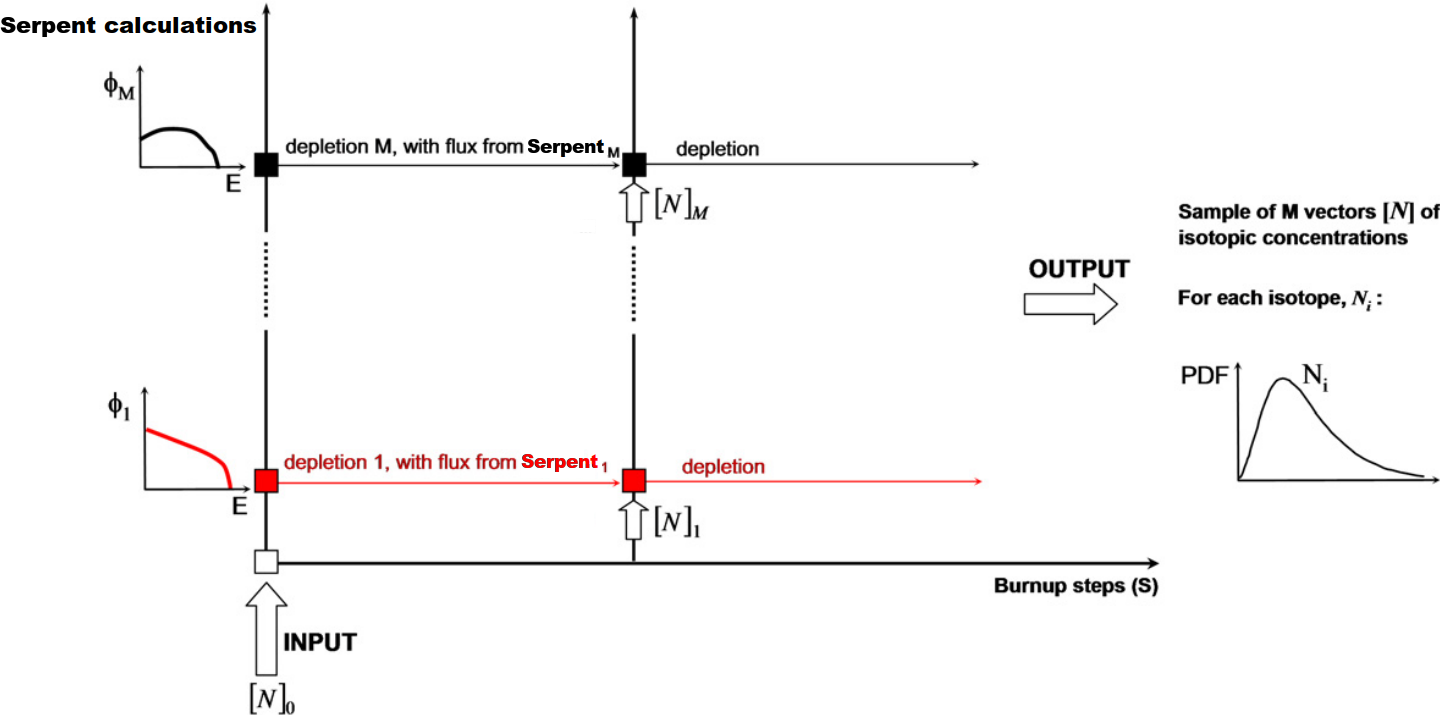
\includegraphics[width=\textwidth]{uq/brute_force_method.png}
	\caption{Methodology of using a normal distribution of random and 
		independent events to estimate uncertainties in final isotopic 
		concentrations (reproduced from Garcia-Herranz \emph{et al.} 
		\cite{garcia-herranz_propagation_2008}). Depletion calculation was 
		performed with the Serpent Monte Carlo code 1000 times by changing only 
		the initial random number.}
	\label{fig:uq-brute-force}
\end{figure}

After running depletion calculations
for all samples, the mean and standard 
deviation of the isotopic concentration can be calculated as
follows
\begin{align}
\overline{N_i} &= \frac{1}{M} \sum_{j=1}^{M} N^{(j)}_i \\
\sigma_{N_i} &= \sqrt{\frac{1}{M-1} \sum_{j=1}^{M} 
	(N^{(j)}_i-\overline{N_j})^2}
\intertext{where}
\overline{N_i} &= \mbox{mean concentration of isotope $i$ $[\frac{1}{cm^3}]$} 
\nonumber \\
M &= \mbox{number of depletion runs with a unique seed $[-]$} 
\nonumber \\
N^{(j)}_i &= \mbox{concentration of isotope $i$ in the sample $j$ 
	$[\frac{1}{cm^3}]$.} 
\nonumber
\end{align}

The isotopic concentration $[N]_j$ can then be propagated throughout the 
criticality calculations to estimate the uncertainty of the multiplication 
factor $k_{eff}$. Serpent Monte Carlo code automatically calculates the mean 
and standard deviation of the $k_{eff}$ in each run $j$, which is 
necessary to find the number of runs (samples) required for the convergence of 
$k_{eff}$.

The \gls{TAP} full-core model in Serpent described earlier (see  
Section~\ref{sec:tap_model}) is used for the uncertainty quantification study 
herein. The model benefits from 1/8 symmetry, which allowed me to 
significantly reduce the computational burden without losing accuracy
(Figure~\ref{fig:tap-serpent-plan}). The number of neutron histories was 
selected to compromise between accuracy and computational costs. Running 
15,000 neutrons with 500 active cycles and 200 inactive cycles 
(used for source convergence) gave a reasonable balance between statistical 
certainty and computation time. Thirty depletion time steps were 
selected for a 30-year depletion simulation (i.e., the isotopic composition is 
stored, and neutron flux is recalculated at the end of each year). 
Additionally, I selected the Chebyshev Rational Approximation Method (CRAM) 
with a predictor-corrector substep \cite{pusa_computing_2010} to reduce 
isotopic 
composition uncertainty. The ENDF/B-VII.1 nuclear data library at 900 K is 
used for all simulations in the current chapter 
\cite{chadwick_endf/b-vii.1_2011}.

\subsection{Results and analysis}
A total of 1000 samples is propagated via the Serpent depletion calculation,  
and the histograms of eigenvalue samples at the \gls{BOL} and \gls{EOL} (30 
\gls{EFPY}) are shown in Figure~\ref{fig:uq-serp-keff-hist}. The 
results show that the mean effective multiplication factor ($k_{eff}$) 
and its standard deviation both decrease gradually during 30 years of 
\gls{TAP} reactor operation due to the stochastic nature of \gls{MC}. 
An uncertainty in $k_{eff}$ of approximately $35$ $pcm$ is observed at the 
\gls{BOL}, while it slipped to about $29$ $pcm$ at the \gls{EOL}. A 1000 
independent Serpent runs were performed on Idaho National Laboratory's Falcon 
supercomputer to obtain a set of M=1000 vectors of isotopic concentrations in 
a depletion simulation with S=30 depletion time intervals each. The 
computational time for such an analysis was approximately 1,200 node-hours 
(4.9 core-years).
\begin{figure}[htp!] % replace 't' with 'b' to 
	\centering
	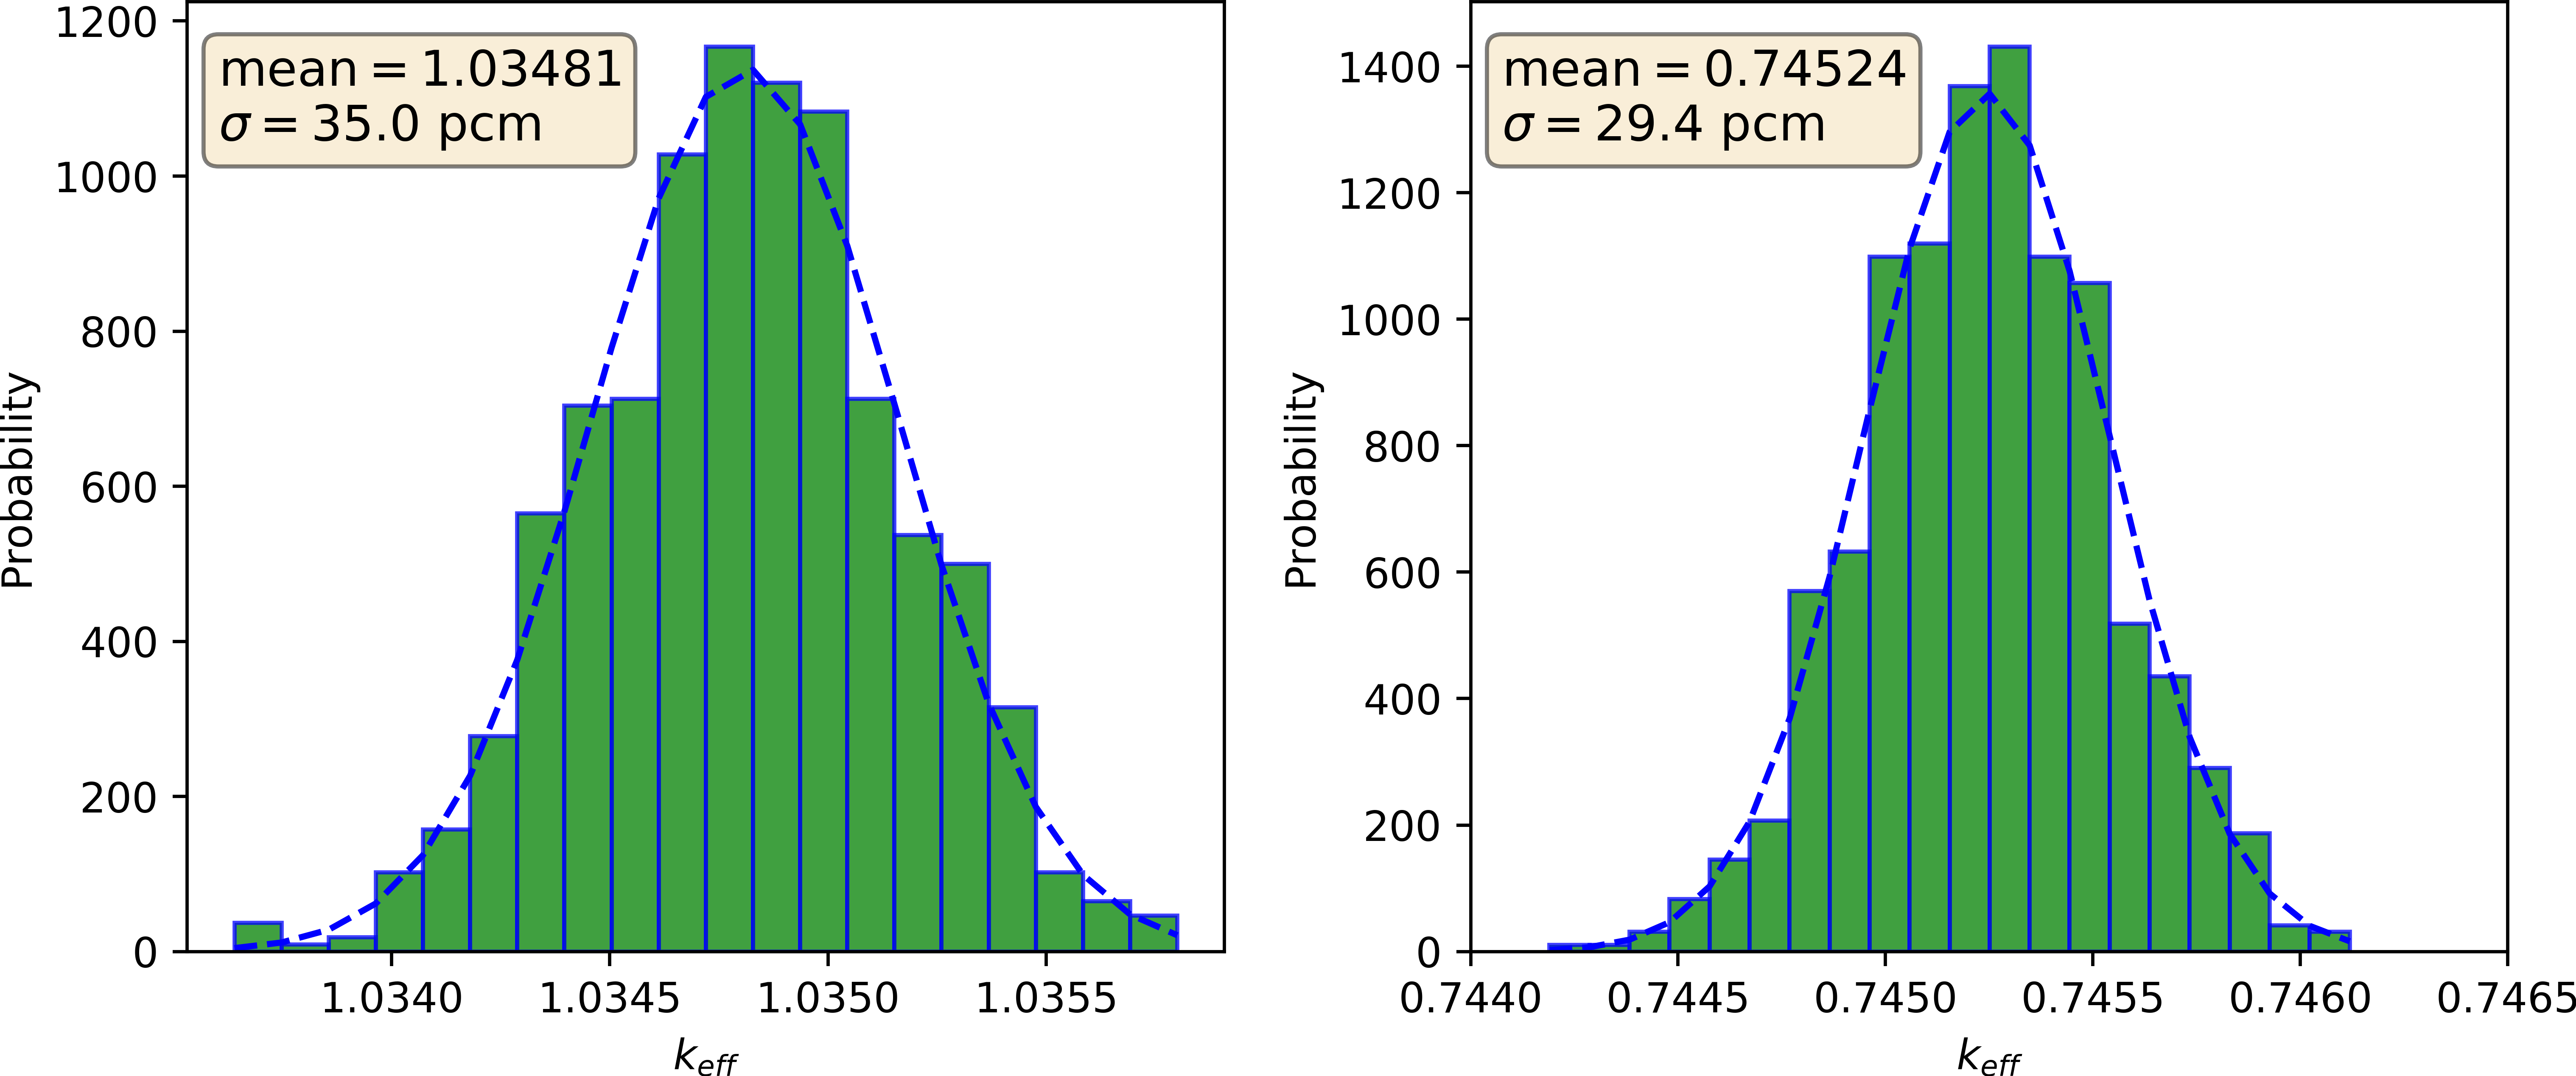
\includegraphics[width=\textwidth]{uq/endf_serpent_keff_hist_for_tap.png}
	\vspace{-4mm}
	\caption{Histograms of $k_{eff}$ samples obtained with 1000 independent 
		Serpent depletion calculations at the \gls{BOL} (left) and \gls{EOL} 
		(right).}
	\label{fig:uq-serp-keff-hist}
\end{figure}

Figure~\ref{fig:uq-serpent-keff-evolution} shows the observed and reported by 
Serpent uncertainties in $k_{eff}$ for the \gls{TAP} core during 30 years of 
operation. Notably, Serpent-calculated uncertainty in the multiplication 
factor is slightly lower than observed uncertainty. This discrepancy is due to 
statistical noise in the pseudo-randomly generated initial seed and agreed 
with results in the literature 
\cite{wyant_numerical_2012}. Across all 30 depletion steps, the mean observed 
and reported uncertainty in the $k_{eff}$ is $30$ and $25$ $pcm$, 
respectively. A better match in these values could be obtained with more 
samples $M$ (e.g., $M=10,\!000$), which would require substantially more 
computational power.
\begin{figure}[hbp!] % replace 't' with 'b' to 
	\centering
	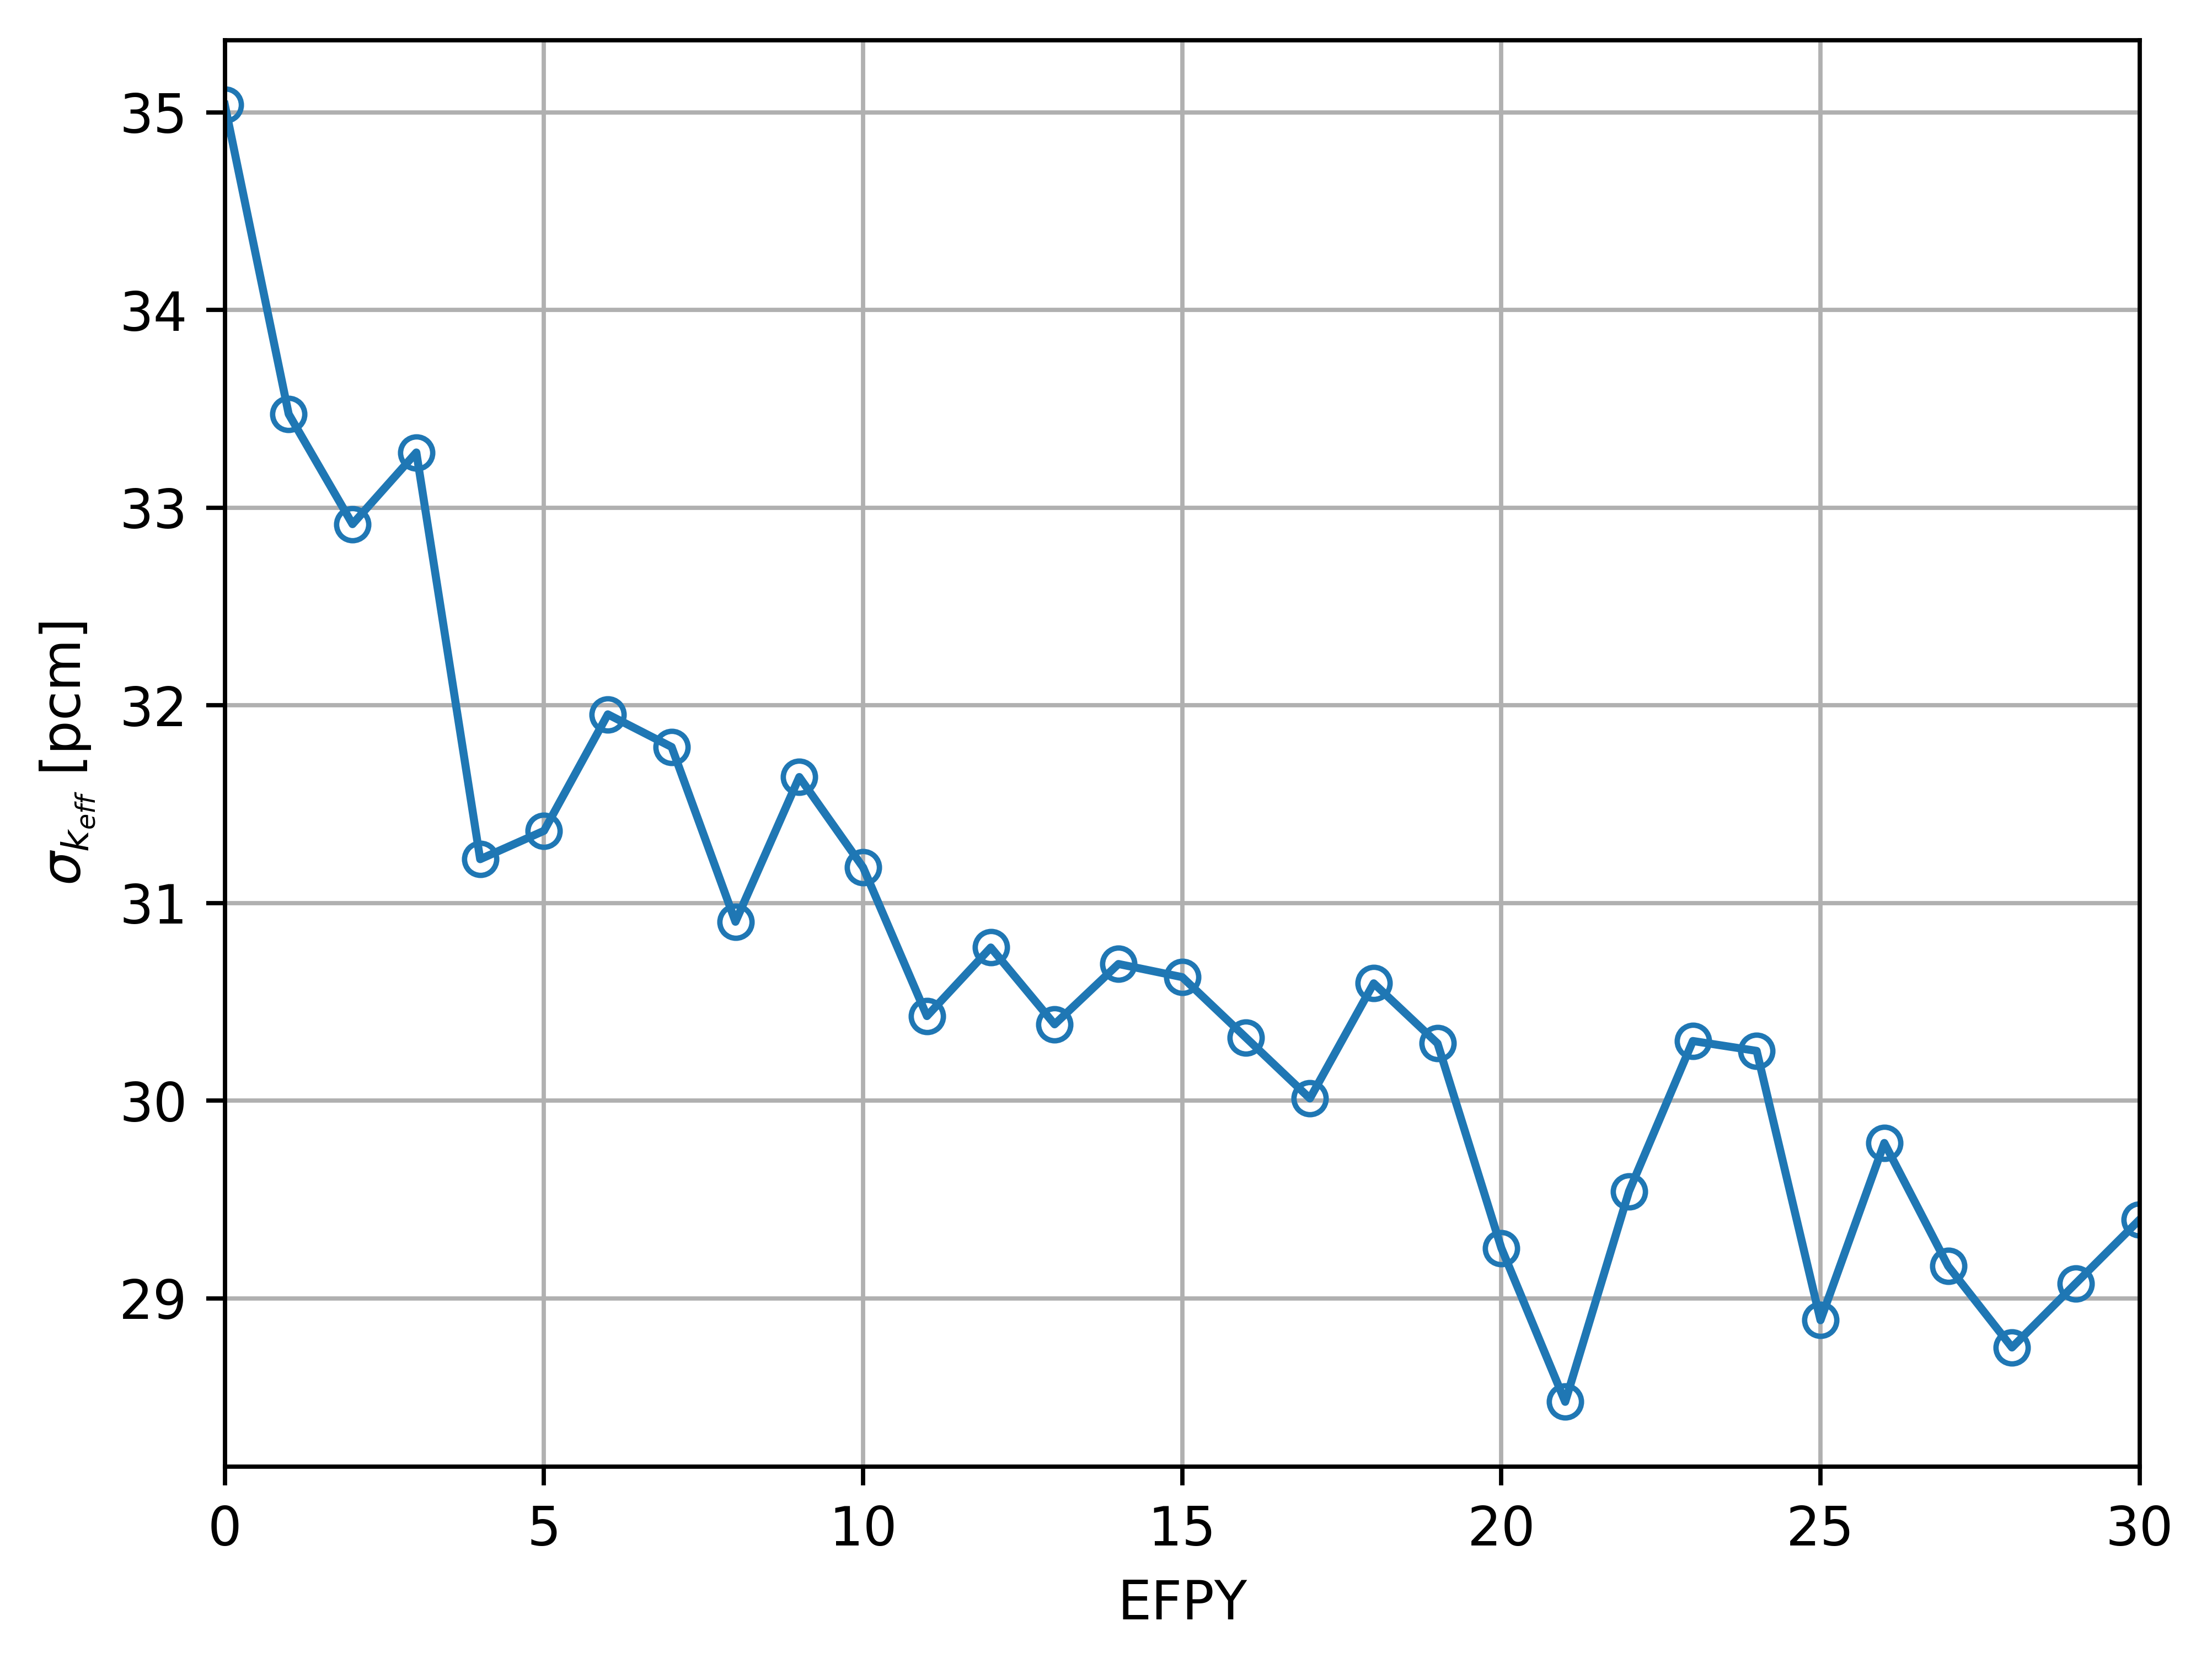
\includegraphics[width=0.83\textwidth]{uq/endf_serpent_keff_dynamics_for_tap.png}
	\caption{Observed and reported by Serpent uncertainty of the effective 
		multiplication factor ($\sigma_{k_{eff}}$) for the full-core \gls{TAP} 
		core model during 30 years of operation.}
	\label{fig:uq-serpent-keff-evolution}
\end{figure}

The current depletion algorithm in Serpent uses the neutron flux solution 
obtained from the \gls{MC} neutron histories to solve the Bateman equations to 
find the isotopic inventory evolution. As was discussed earlier, Serpent 
is unable to estimate the uncertainty of the isotopic number density like it 
does for the $k_{eff}$ (reported $\sigma_{k_{eff}}$ in 
Figure~\ref{fig:uq-serpent-keff-evolution}). Thus, to gain insight into the 
uncertainties in the isotopic inventory, the standard deviation in observed 
isotopic inventories from the 1000 depletion runs was investigated. The 
observed uncertainties for the major actinides and poisonous \glspl{FP} 
resulting from depletion calculations are shown on  
Figures~\ref{fig:uq-serpent-u}, \ref{fig:uq-serpent-pu}, and 
\ref{fig:uq-serpent-xe-i}.

\begin{figure}[htp!] % replace 't' with 'b' to 
	\centering
	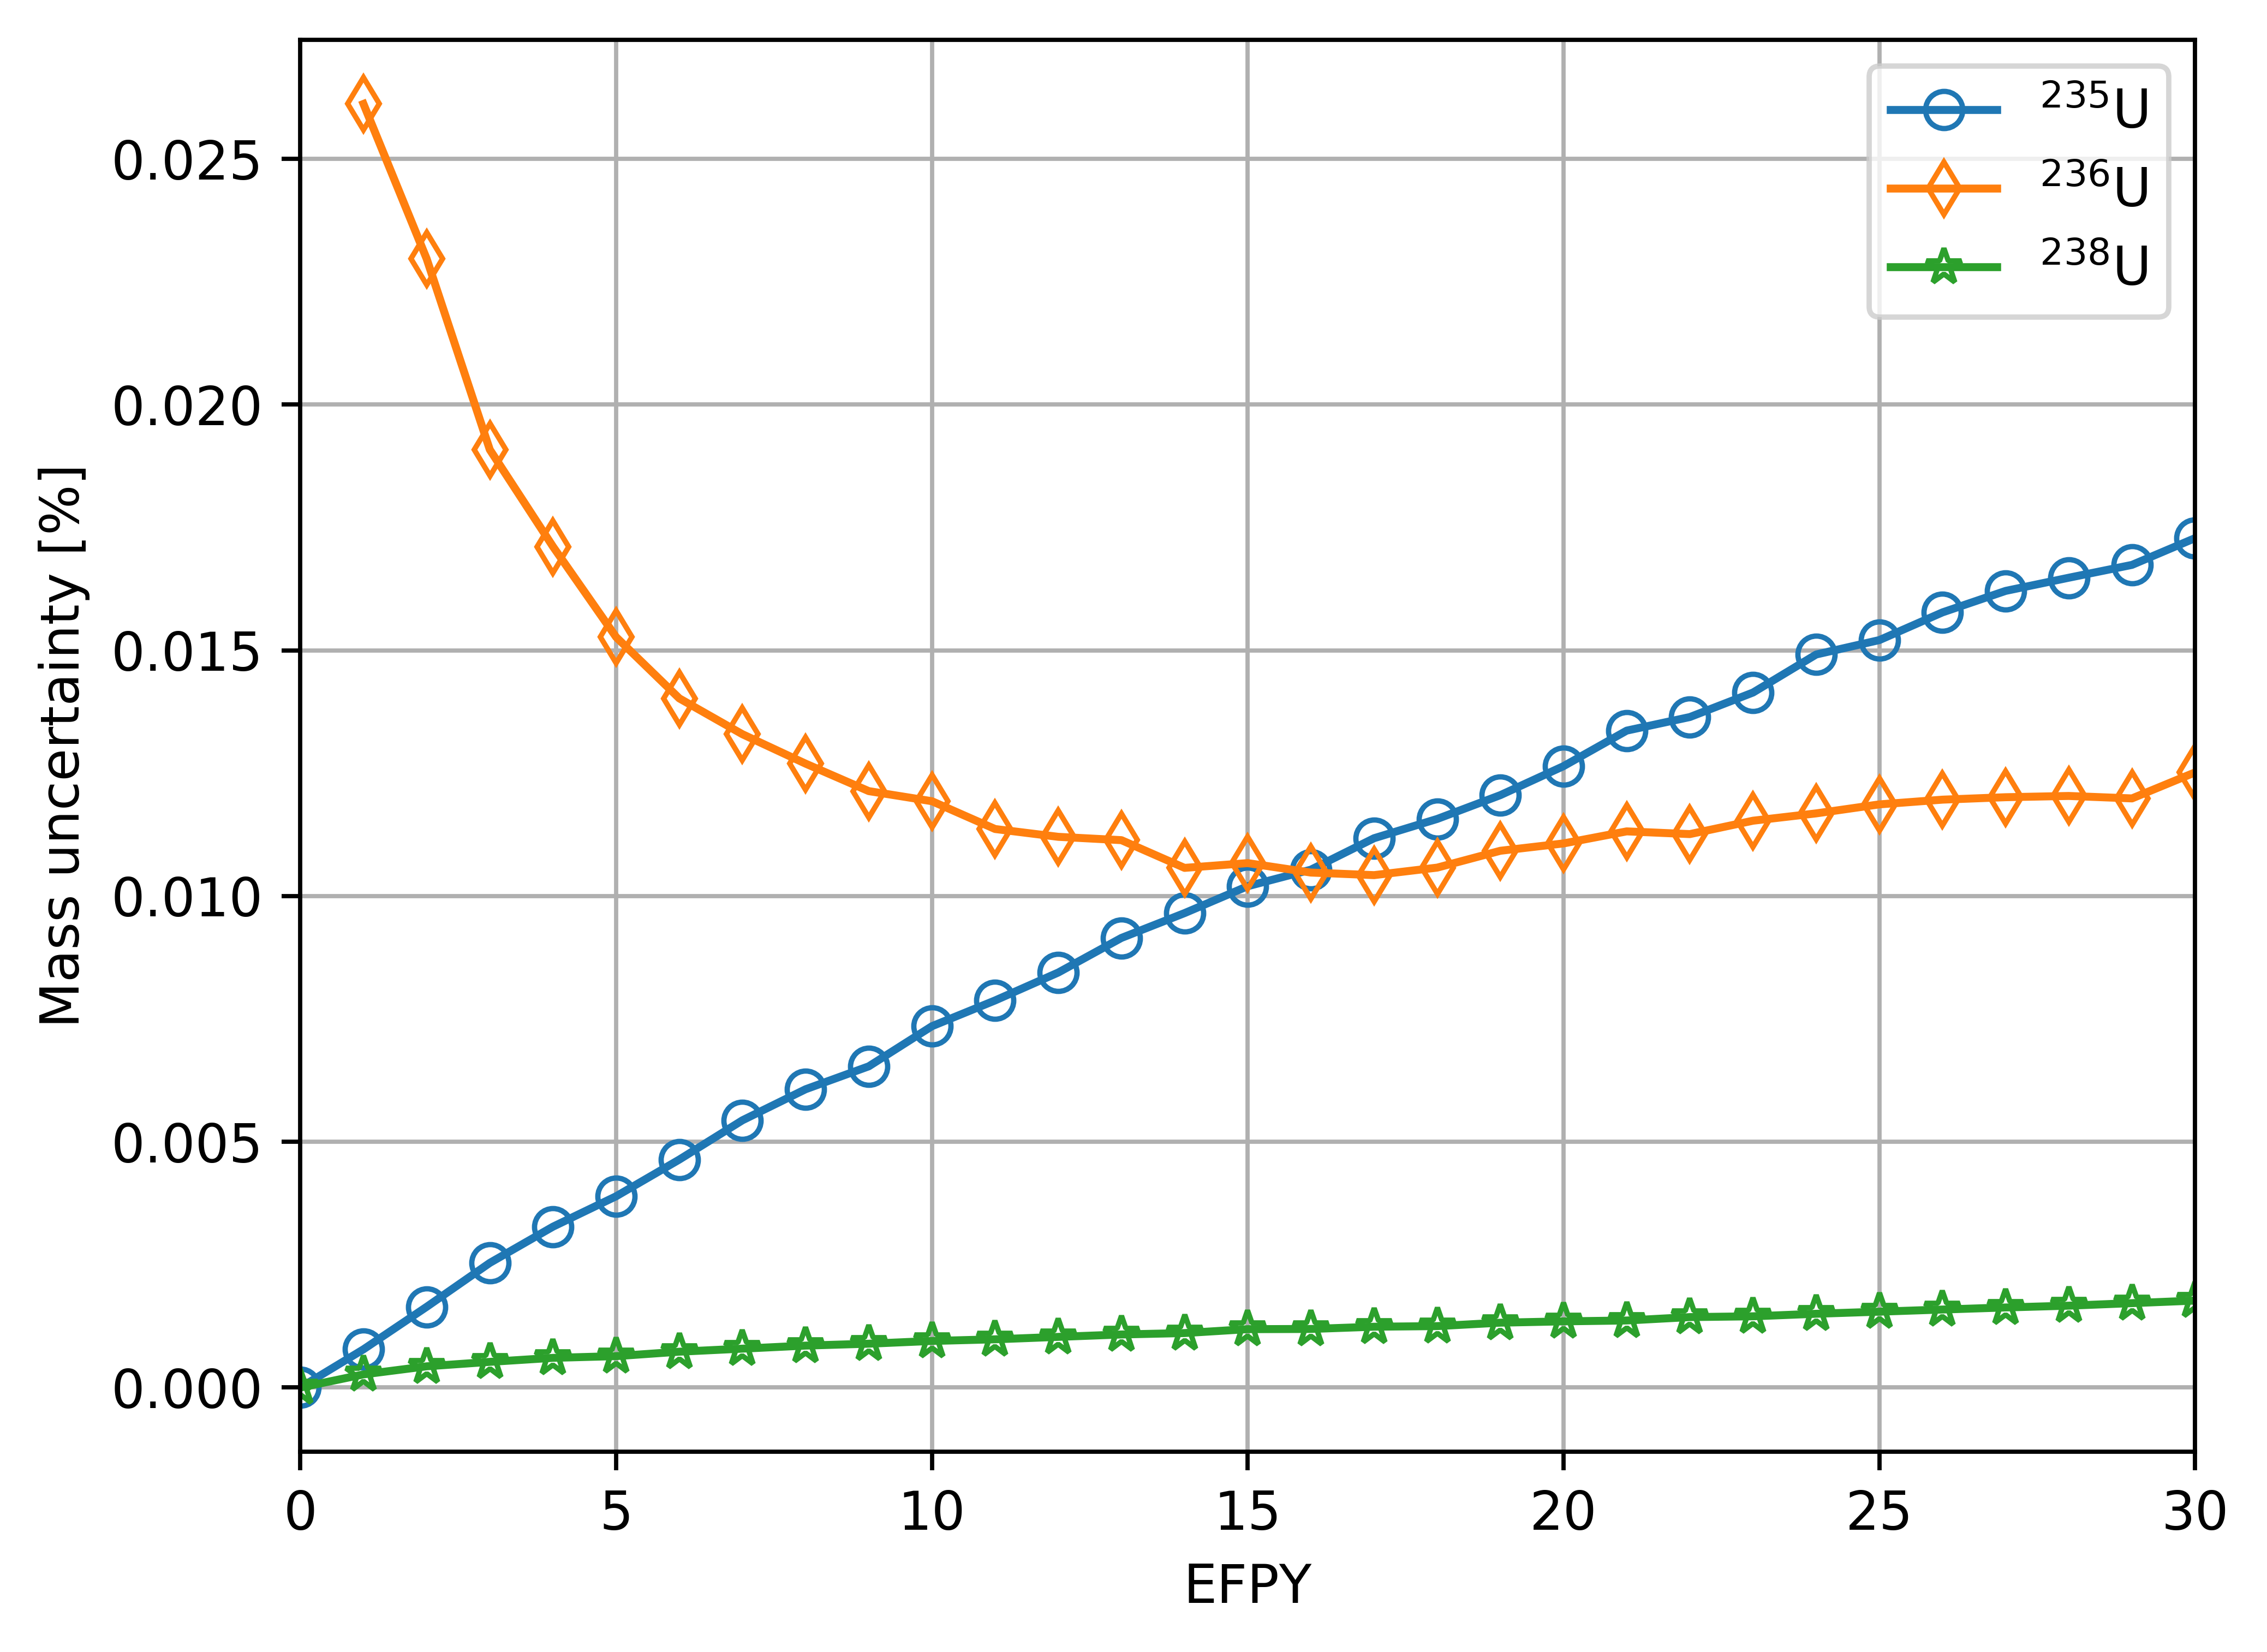
\includegraphics[width=0.8\textwidth]{uq/serpent_mass_std_u.png}
	\vspace{-4mm}
	\caption{Stochastic uncertainty evolution in the uranium isotopic 
		inventory during 30 years of depletion.}
	\label{fig:uq-serpent-u}
\end{figure}

The relative uncertainty of $^{235}$U mass increases with time due to its 
depletion, as the uranium enrichment steadily decreases from 5\% to 0.7\%.
The uncertainty of $^{236}$U mass is 
0.026\% after 30 days of operation when only a few grams of this isotope were 
produced in the core. The uncertainty of $^{236}$U is between 0.011\% and 
0.013\% once the $^{236}$U approaches its equilibrium concentration. The 
relative uncertainties of fissile $^{239}$Pu and $^{241}$Pu are 0.01-0.07\% 
and 0.04-0.18\%, respectively. Mass uncertainties for the 
strongest neutron poison, $^{135}$Xe, and its primary direct precursor, 
$^{135}$I, are 0.0175-0.0275\% and 0.01-0.0175\%, respectively. Overall, 
stochastic error in depletion calculations is larger for isotopes with small 
concentrations in the core due to round-off error. 
Table~\ref{tab:uq-serpent-mean-std-rsd} shows that the stochastic error in the 
isotopic inventories even for an unusually high burnup of 100 MW$_{th}$d/kgU 
(30 EFPY) is negligible ($<0.1$\%).

\begin{figure}[htp!] % replace 't' with 'b' to 
	\centering
	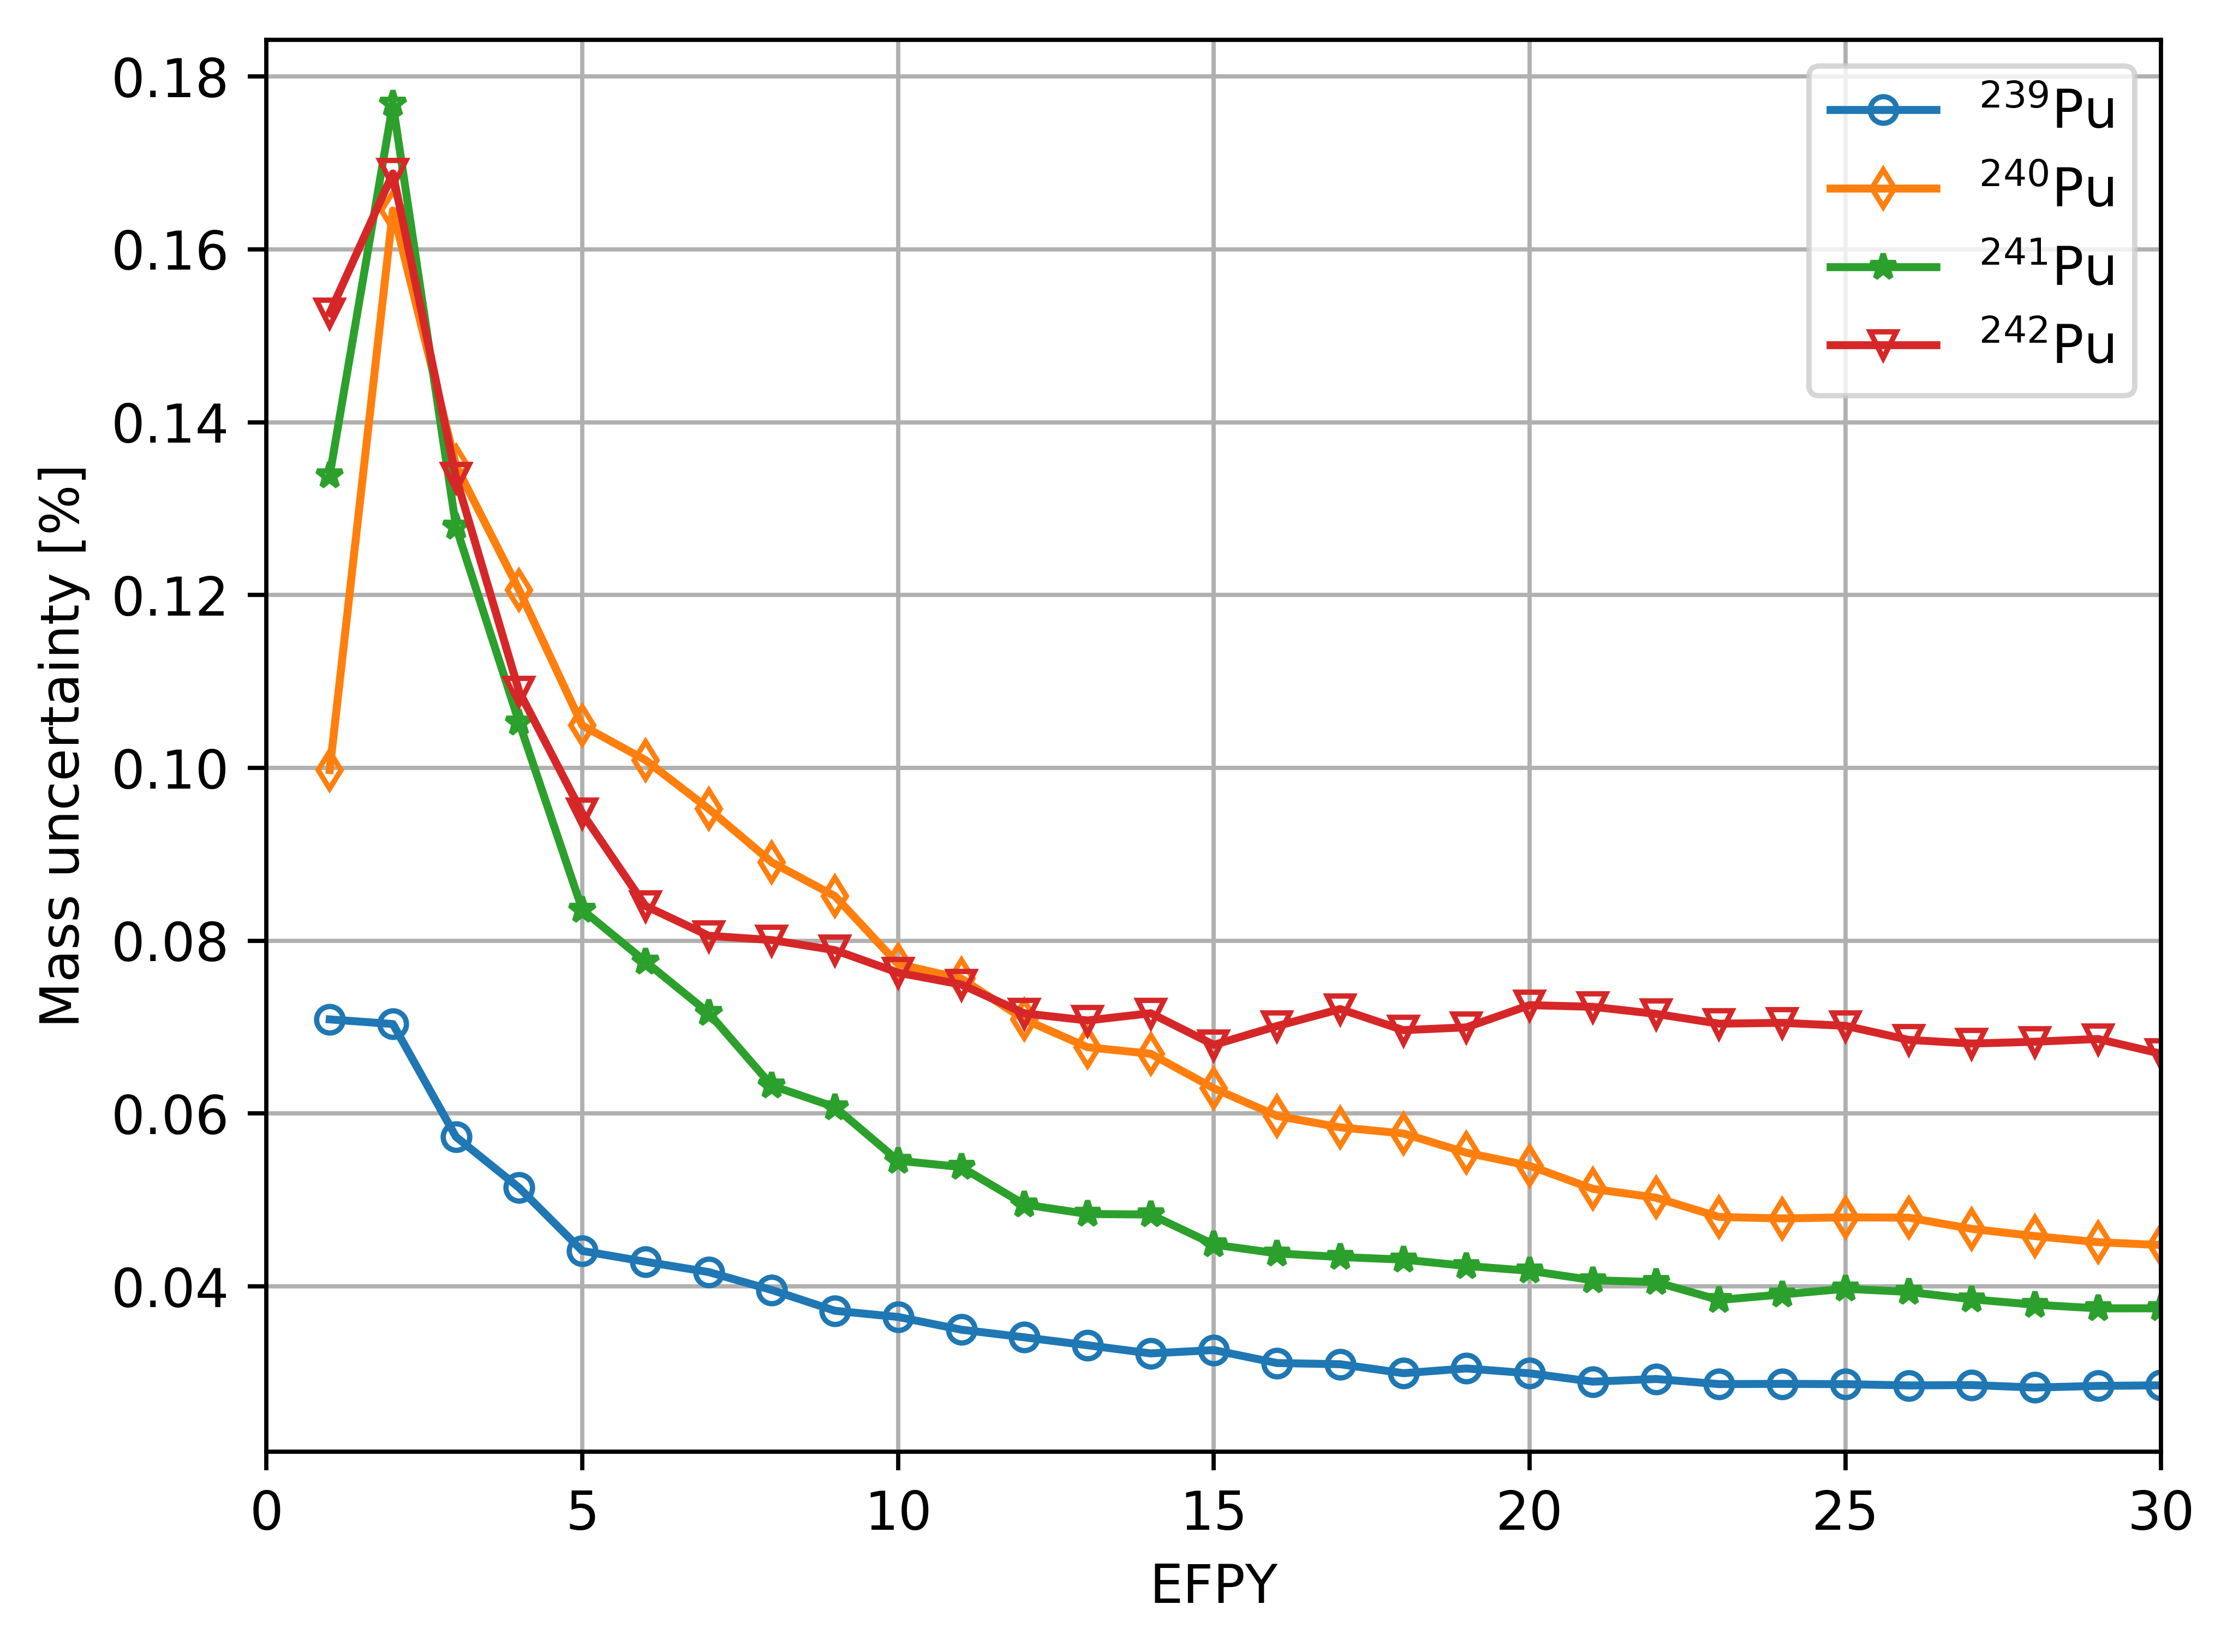
\includegraphics[width=0.73\textwidth]{uq/serpent_mass_std_pu.png}
	\vspace{-3mm}
	\caption{Stochastic uncertainty evolution in the plutonium isotopic 
		inventory during 30 years of depletion.}
	\label{fig:uq-serpent-pu}
\end{figure}
\vspace{-9mm}
\begin{figure}[hbp!] % replace 't' with 'b' to 
	\centering
	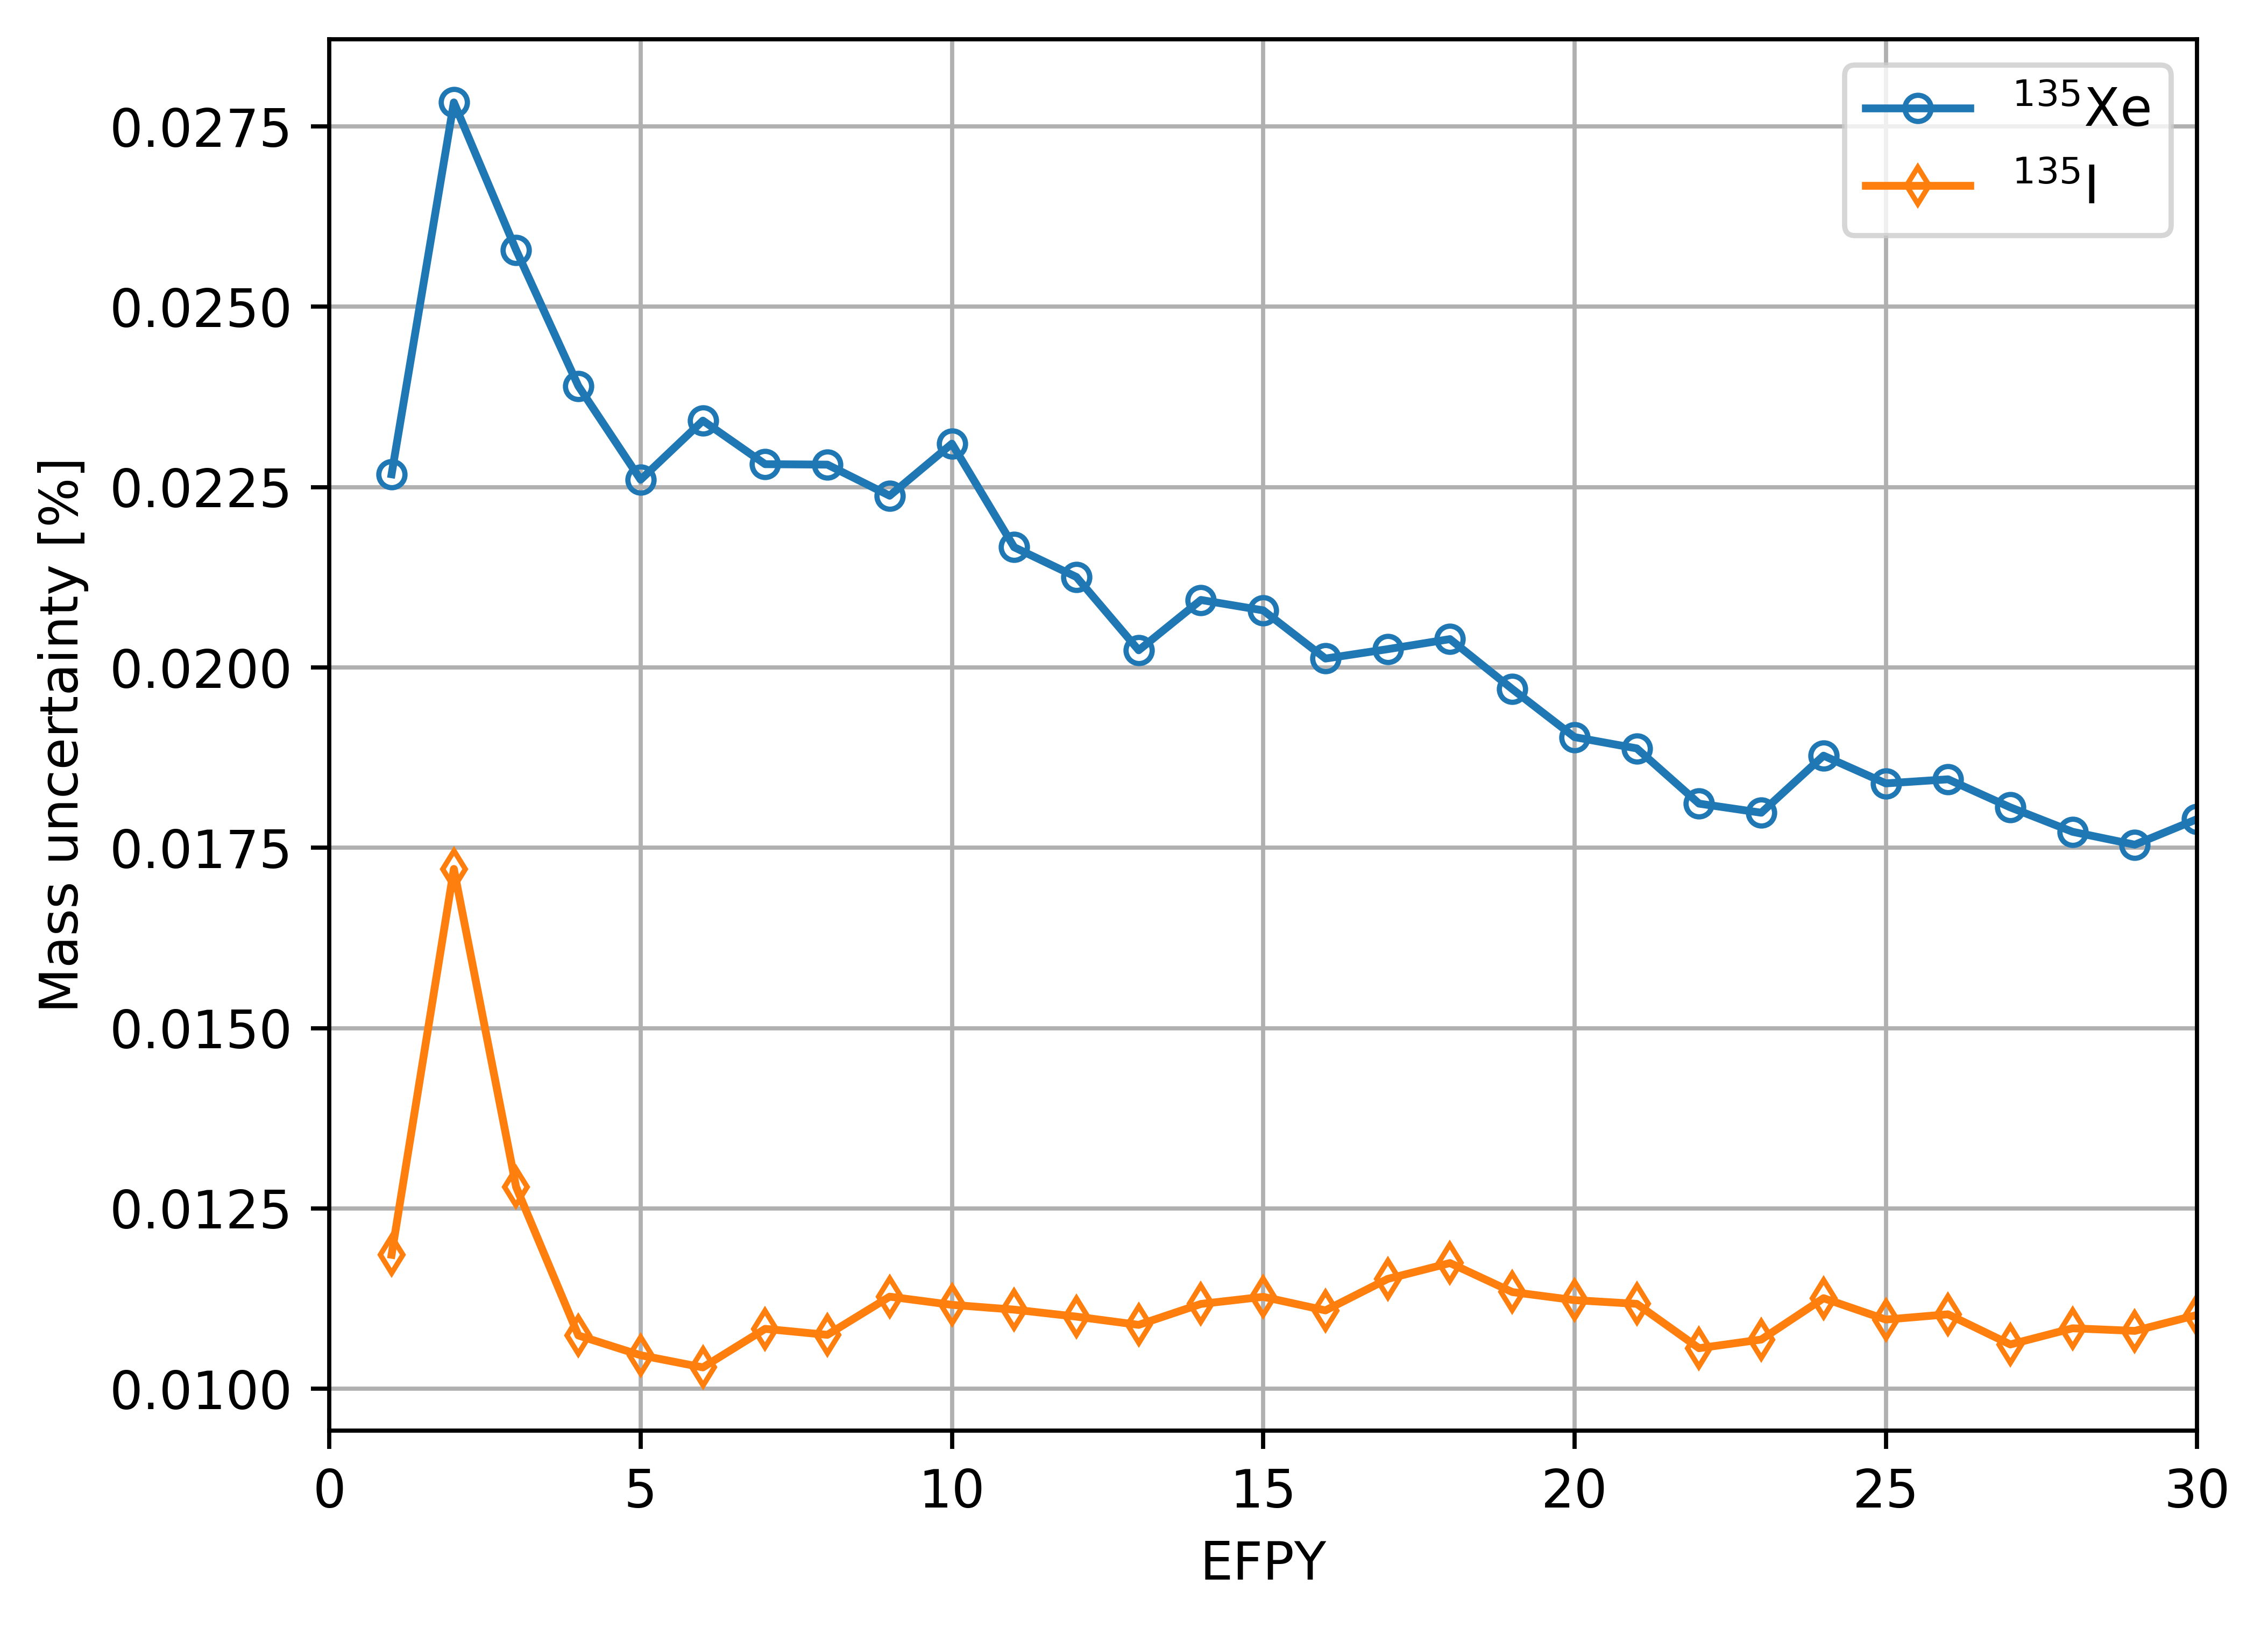
\includegraphics[width=0.73\textwidth]{uq/serpent_mass_std_xe_i.png}
	\vspace{-3mm}
	\caption{Stochastic uncertainty evolution in $^{135}$Xe and $^{135}$I 
		isotopic inventory during 30 years of depletion.}
	\label{fig:uq-serpent-xe-i}
\end{figure}


%%%%%%%%%%%%%%%%%%%%%%%%%%%%%%%%%%%%%%%%
\begin{table}[htp!]
	\centering
	\caption{Mean value, Standard Deviation (STD), and Relative Standard 
		Deviation (RSD) of mass for the major isotopes after 30-year depletion 
		analysis for the \gls{TAP} reactor. Only the stochastic error in the 
		Monte 
		Carlo calculations is considered.}
	\begin{tabularx}{0.7\textwidth}{L R R R R}
		\hline
		\textbf{Isotope}  & \textbf{Mean ($\mu$) [kg]} & \textbf{STD 
			($\sigma$) [kg]} & \textbf{RSD ($\sigma/\mu$) [\%]}\\ \hline
		$^{234}$U  & 25.8  & 0.0075 & 0.0290\% \\
		$^{235}$U  & 789.9 & 0.1365 & 0.0173\% \\
		$^{236}$U  & 1149.5& 0.1439 & 0.0125\% \\
		$^{238}$U  & 112,084.8 & 1.9835 & 0.0018\% \\
		$^{238}$Pu & 405.5 & 0.0884 & 0.0218\% \\
		$^{239}$Pu & 5554.3& 1.5860 & 0.0286\% \\
		$^{240}$Pu & 1230.2& 0.5510 & 0.0448\% \\
		$^{241}$Pu & 763.1 & 0.2859 & 0.0375\% \\
		$^{242}$Pu & 139.0 & 0.0930  & 0.0669\% \\
		$^{241}$Am & 218.3 & 0.0566  & 0.0259\% \\
		$^{135}$Xe & 0.03  & $<0.0001$& 0.0179\% \\
		$^{135}$I  & 0.02  & $<0.0001$& 0.0110\% \\ \hline
	\end{tabularx}
	\label{tab:uq-serpent-mean-std-rsd}
	\vspace{-0.9em}
\end{table}
%%%%%%%%%%%%%%%%%%%%%%%%%%%%%%%%%%%%%%%%%%%%%%%%%%%%%%%%%%%%%%%%%%%%%%%%%%%%%%%

All results presented in Figures~\ref{fig:uq-serpent-u},  
\ref{fig:uq-serpent-pu}, \ref{fig:uq-serpent-xe-i}, and  
Table~\ref{tab:uq-serpent-mean-std-rsd} are based on 1000 samples (e.g., 1000 
independent Serpent depletion simulations with unique random seeds). 
Figure~\ref{fig:uq-serpent-convergence} shows the 
convergence of $k_{eff}$ and $^{235}$U mass uncertainty with the number of 
samples. Notably, 300 samples were enough for $\sigma_{k_{eff}}$ convergence. 
The $^{235}$U mass uncertainty at the \gls{EOL} decreases steadily 
with the number of samples, but even 400 samples are sufficient to obtain 
reasonable uncertainty ($<0.02$\%). 
Finally, it is possible to reduce the stochastic uncertainty in the isotopic 
inventory to almost zero by substantially increasing the neutron population 
(number of neutron histories and active cycles). However, this is extremely 
inefficient because Monte Carlo converges sublinearly ($O(\sqrt{N})$).
\begin{figure}[htp!] % replace 't' with 'b' to 
	\centering
	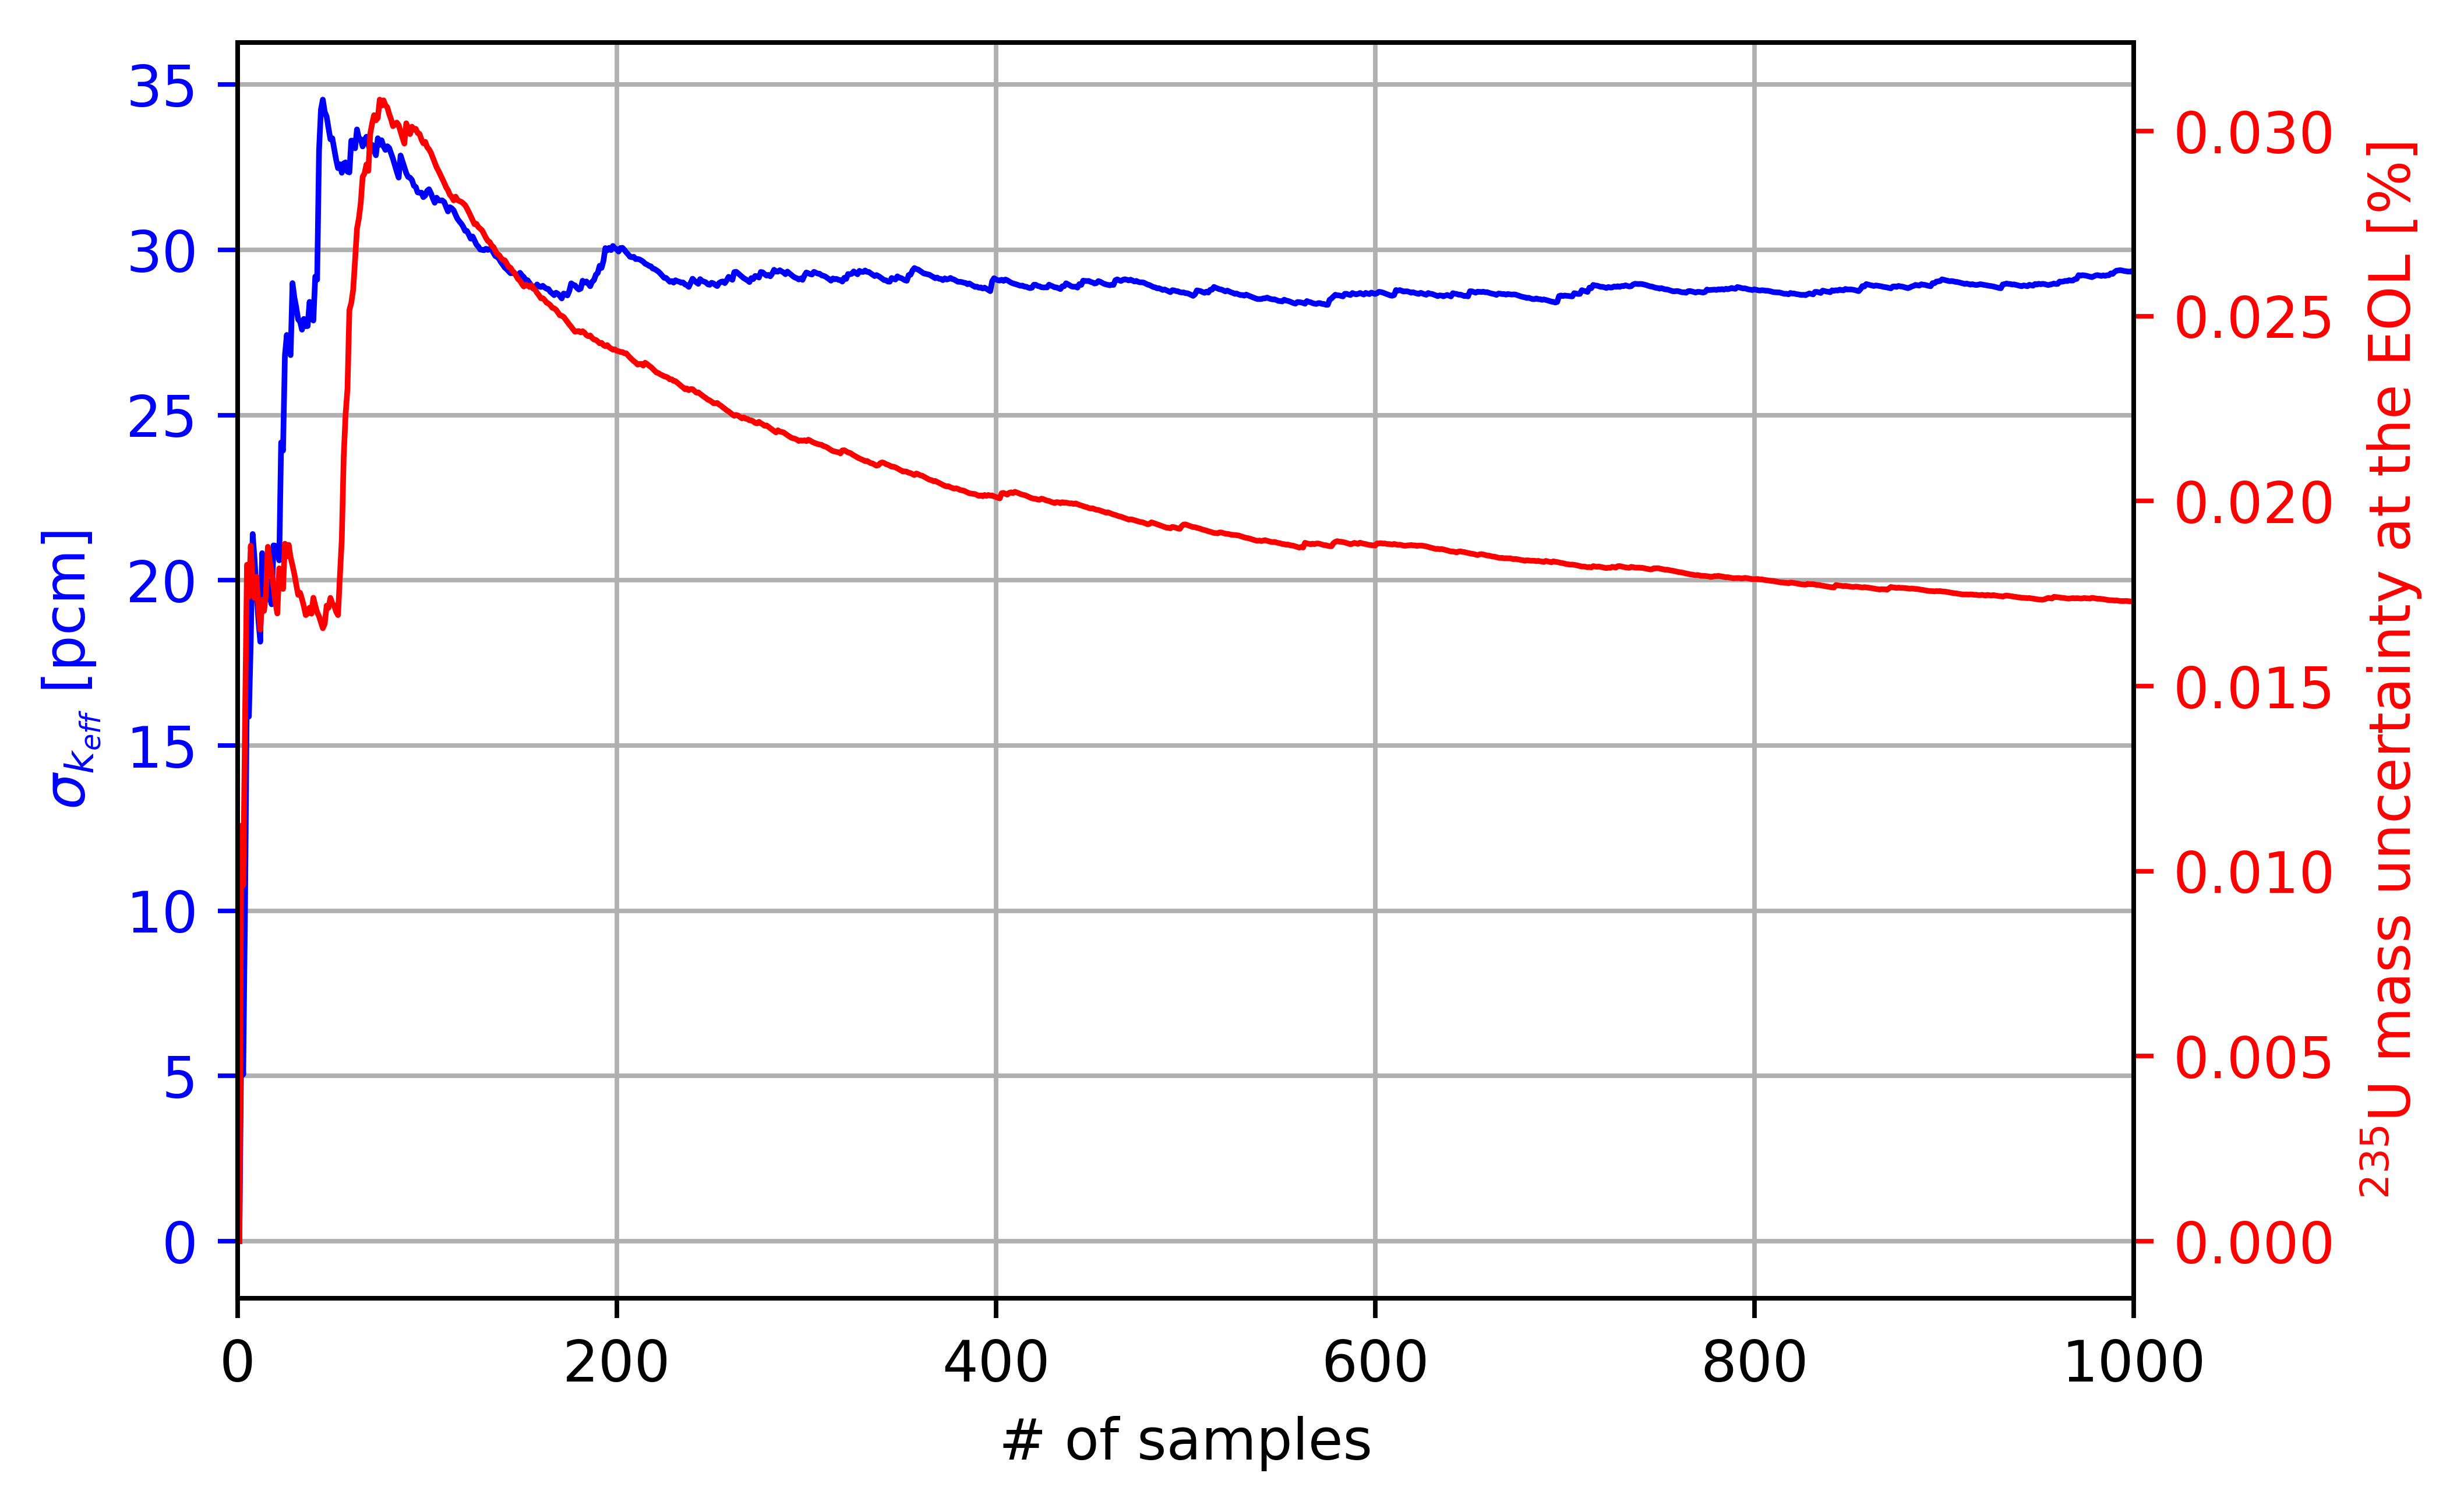
\includegraphics[width=\textwidth]{uq/serpent_convergance_for_tap.png}
	\caption{Convergence of $k_{eff}$ and $^{235}$U mass uncertainties due to 
		the statistical error in Monte Carlo as a function of number of 
		samples.}
	\label{fig:uq-serpent-convergence}
\end{figure}
\FloatBarrier


\section{Nuclear data-related uncertainty in the isotopic inventory}
This section focuses on evaluating uncertainty in a depletion calculation 
caused by uncertainties in nuclear data, namely, cross sections, fission 
yields, and decay constants. I used a deterministic $S_N$ transport solver, 
SCALE/TRITON \cite{rearden_scale_2018}, to avoid statistical errors and 
isolate nuclear data-related uncertainty.

\subsection{Methodology of uncertainty propagation by a random sampling}
Nuclear data uncertainties are propagated through fuel depletion calculations 
using a random sampling method\footnote{Sometimes researchers also 
	called it ``Monte Carlo sampling," \cite{radaideh_using_2019} ``brute 
	force method,"\cite{garcia-herranz_propagation_2008} or ``Fast Total Monte 
	Carlo" \cite{rochman_nuclear_2014}. However, in this chapter, this method 
	is 
	called ``random  sampling."}. The multi-step sequence of deterministic 
neutronics and isotopic transmutation could be regarded as a single 
process with input parameters (cross sections, fission yields, decay 
constants) and an output (isotopic inventory). This sequence runs a 
large number of times, each time using a different nuclear data file (sample). 
This collection of random nuclear data files is produced by the SCALE Sampler 
module from a multivariate normal distribution using covariance matrices in 
the 56-group covariance library \cite{rearden_scale_2018, 
	radaideh_novel_2019}. This approach is summarized in the flowchart 
(Figure~\ref{fig:uq-sampler}).

After generating the collection of random nuclear data files, SCALE performs 
depletion calculations for each sample. This work uses NEWT, a
2D-deterministic transport code, coupled with ORIGEN. ORIGEN solves a set of 
the Bateman equations using NEWT-calculated neutron fluxes. The unit cell 
model is used to achieve reasonable computing costs while providing an 
accurate neutron spectrum for depletion calculations 
(Figure~\ref{fig:uq-tap-pincell}) \cite{betzler_molten_2017, 
	rykhlevskii_fuel_2019, betzler_modeling_2020}. For this unit cell model, an 
8$\times$8 mesh with reflective boundary conditions is used. The 56-group 
ENDF/B-VII.1 nuclear data library along with the 56-group covariance library 
are used in these depletion calculations. 
%The full-core 3-D depletion 
%calculation can be performed if NEWT is replaced with KENO-VI, which 
%is a three-dimensional Monte Carlo neutron transport code, that might be 
%coupled with ORIGEN for performing depletion calculations. However, two 
%reasons make it impractical because: 
%(1) it requires enormous computing cost, (2) it introduces stochastic error 
%due to the statistical nature of the \gls{MC} method, and 
%(3) it cannot be applied to continuous energy Monte Carlo calculations 
%\cite{rearden_scale_2018}.
\begin{figure}[htp!] % replace 't' with 'b' to 
	\centering
	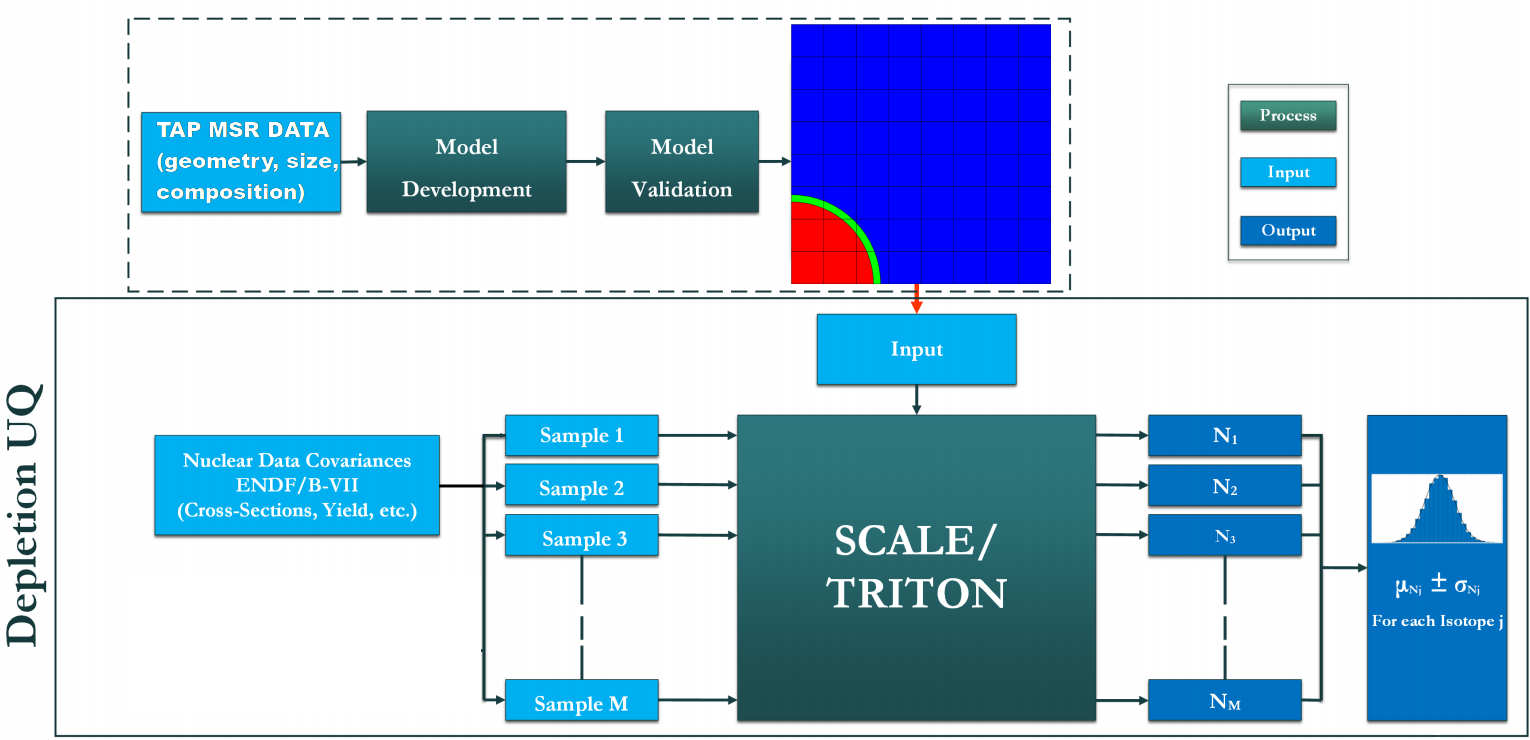
\includegraphics[width=\textwidth]{uq/majdi_scale_scheme.png}
	\caption{Flowchart of depletion uncertainty quantification 
		using SCALE Sampler (figure courtesy of Majdi I. Radaideh 
		\cite{radaideh_novel_2019}).}
	\label{fig:uq-sampler}
\end{figure}
\vspace{-7mm}
\begin{figure}[hbp!] % replace 't' with 'b' to 
	\centering
	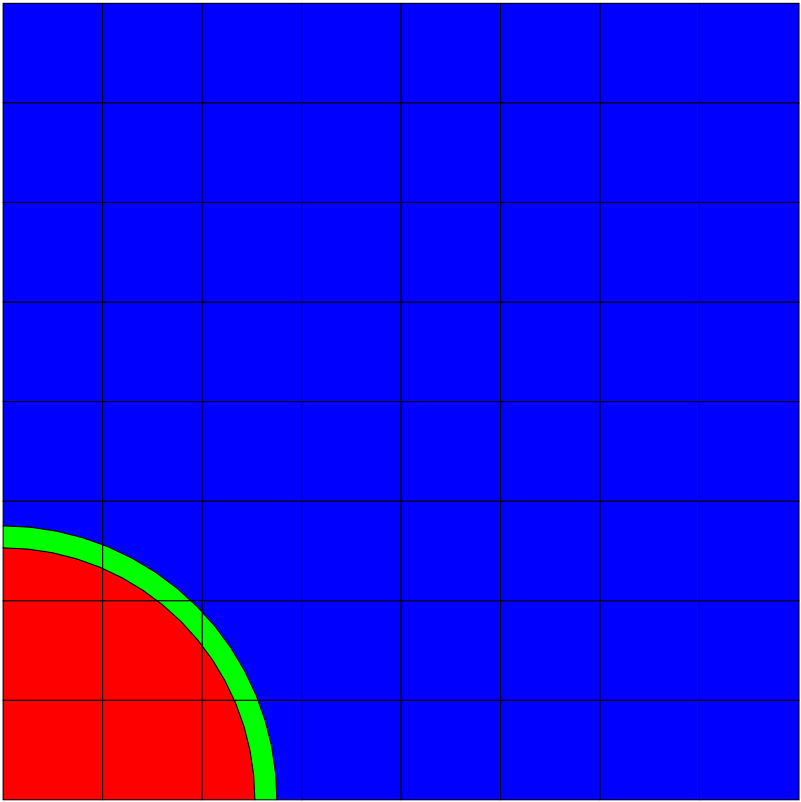
\includegraphics[width=0.41\textwidth]{uq/tap_pin_for_scale.png}
	\caption{Unit cell model representation for the \gls{TAP} \gls{MSR} in 
		SCALE.}
	\label{fig:uq-tap-pincell}
\end{figure}

The fuel salt composition, total depletion time, depletion time steps, and 
power density match the ones given in Section~\ref{sec:uq-stochastic} for 
consistency of comparison. Overall, I repeated 800 SCALE depletion 
calculations using perturbed cross sections, fission yields, and decay 
constants, assuming that the probability density functions are multivariate 
normal distributions with covariances provided with the SCALE nuclear data 
library.


\subsection{Results and analysis}
Figure~\ref{fig:uq-scale-kinf-hist} shows histograms of the 
infinite multiplication factor ($k_{\infty}$) at the \gls{BOL} and \gls{EOL} 
(30 \gls{EFPY}) for 800 total random samples. Similar to stochastic 
uncertainty, the results show that the $k_{\infty}$ standard deviation due to 
the nuclear data uncertainty decreases during 30 years of the \gls{TAP} 
reactor operation. An uncertainty of about 804 $pcm$ in $k_{\infty}$ is 
observed at startup, while it is reduced to 469 $pcm$ at the \gls{EOL}. 
Notably, nuclear data-related uncertainty in the multiplication factor is 
about 20 times larger than uncertainty due to the stochastic error (see 
Section~\ref{sec:uq-stochastic}), which agrees well with results in the 
literature \cite{takeda_estimation_1999, garcia-herranz_propagation_2008}. 
Thanks to the unit cell model and a fast deterministic $S_N$ NEWT transport 
code, the computational time for producing 800 random samples was only 576 
core-days. Generation of the 800 samples with better accuracy (full-core, 
three-dimensional model solved with KENO-VI) would require substantially more 
computational power (about 10,000 times more).
\begin{figure}[htp!] % replace 't' with 'b' to 
	\centering
	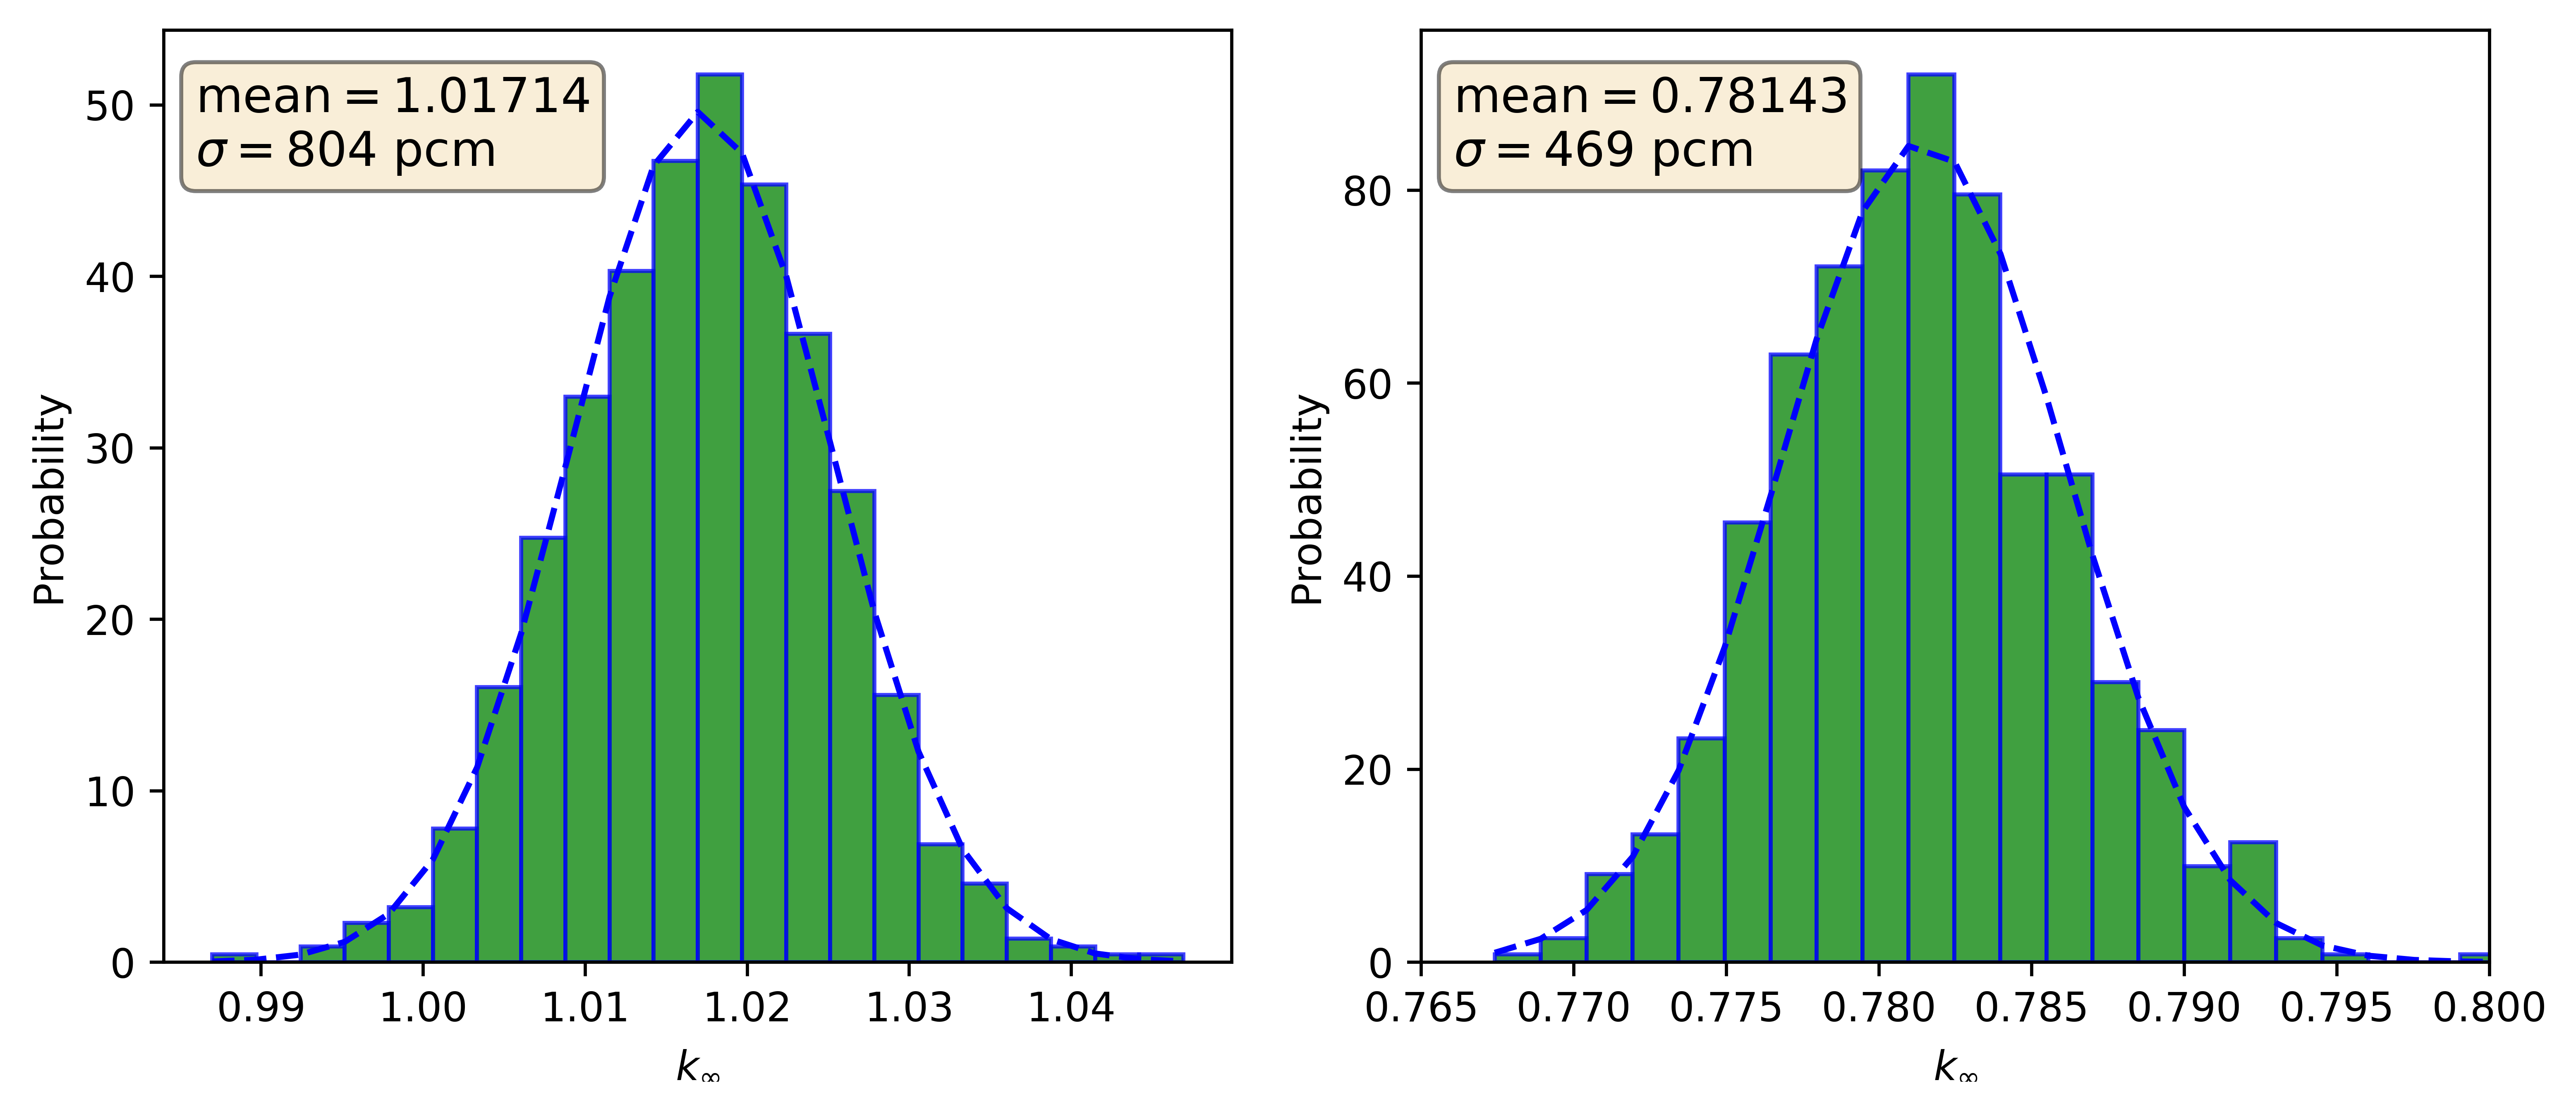
\includegraphics[width=\textwidth]{uq/endf_scale_keff_hist_for_tap.png}
	\vspace{-8mm}
	\caption{Histograms of $k_{\infty}$ at the \gls{BOL} (left) and 
		\gls{EOL} (right) obtained with SCALE Sampler by stochastically 
		sampling the nuclear data (cross sections, fission yields, decay 
		constants).}
	\label{fig:uq-scale-kinf-hist}
\end{figure}
\begin{figure}[hbp!] % replace 't' with 'b' to 
	\centering
	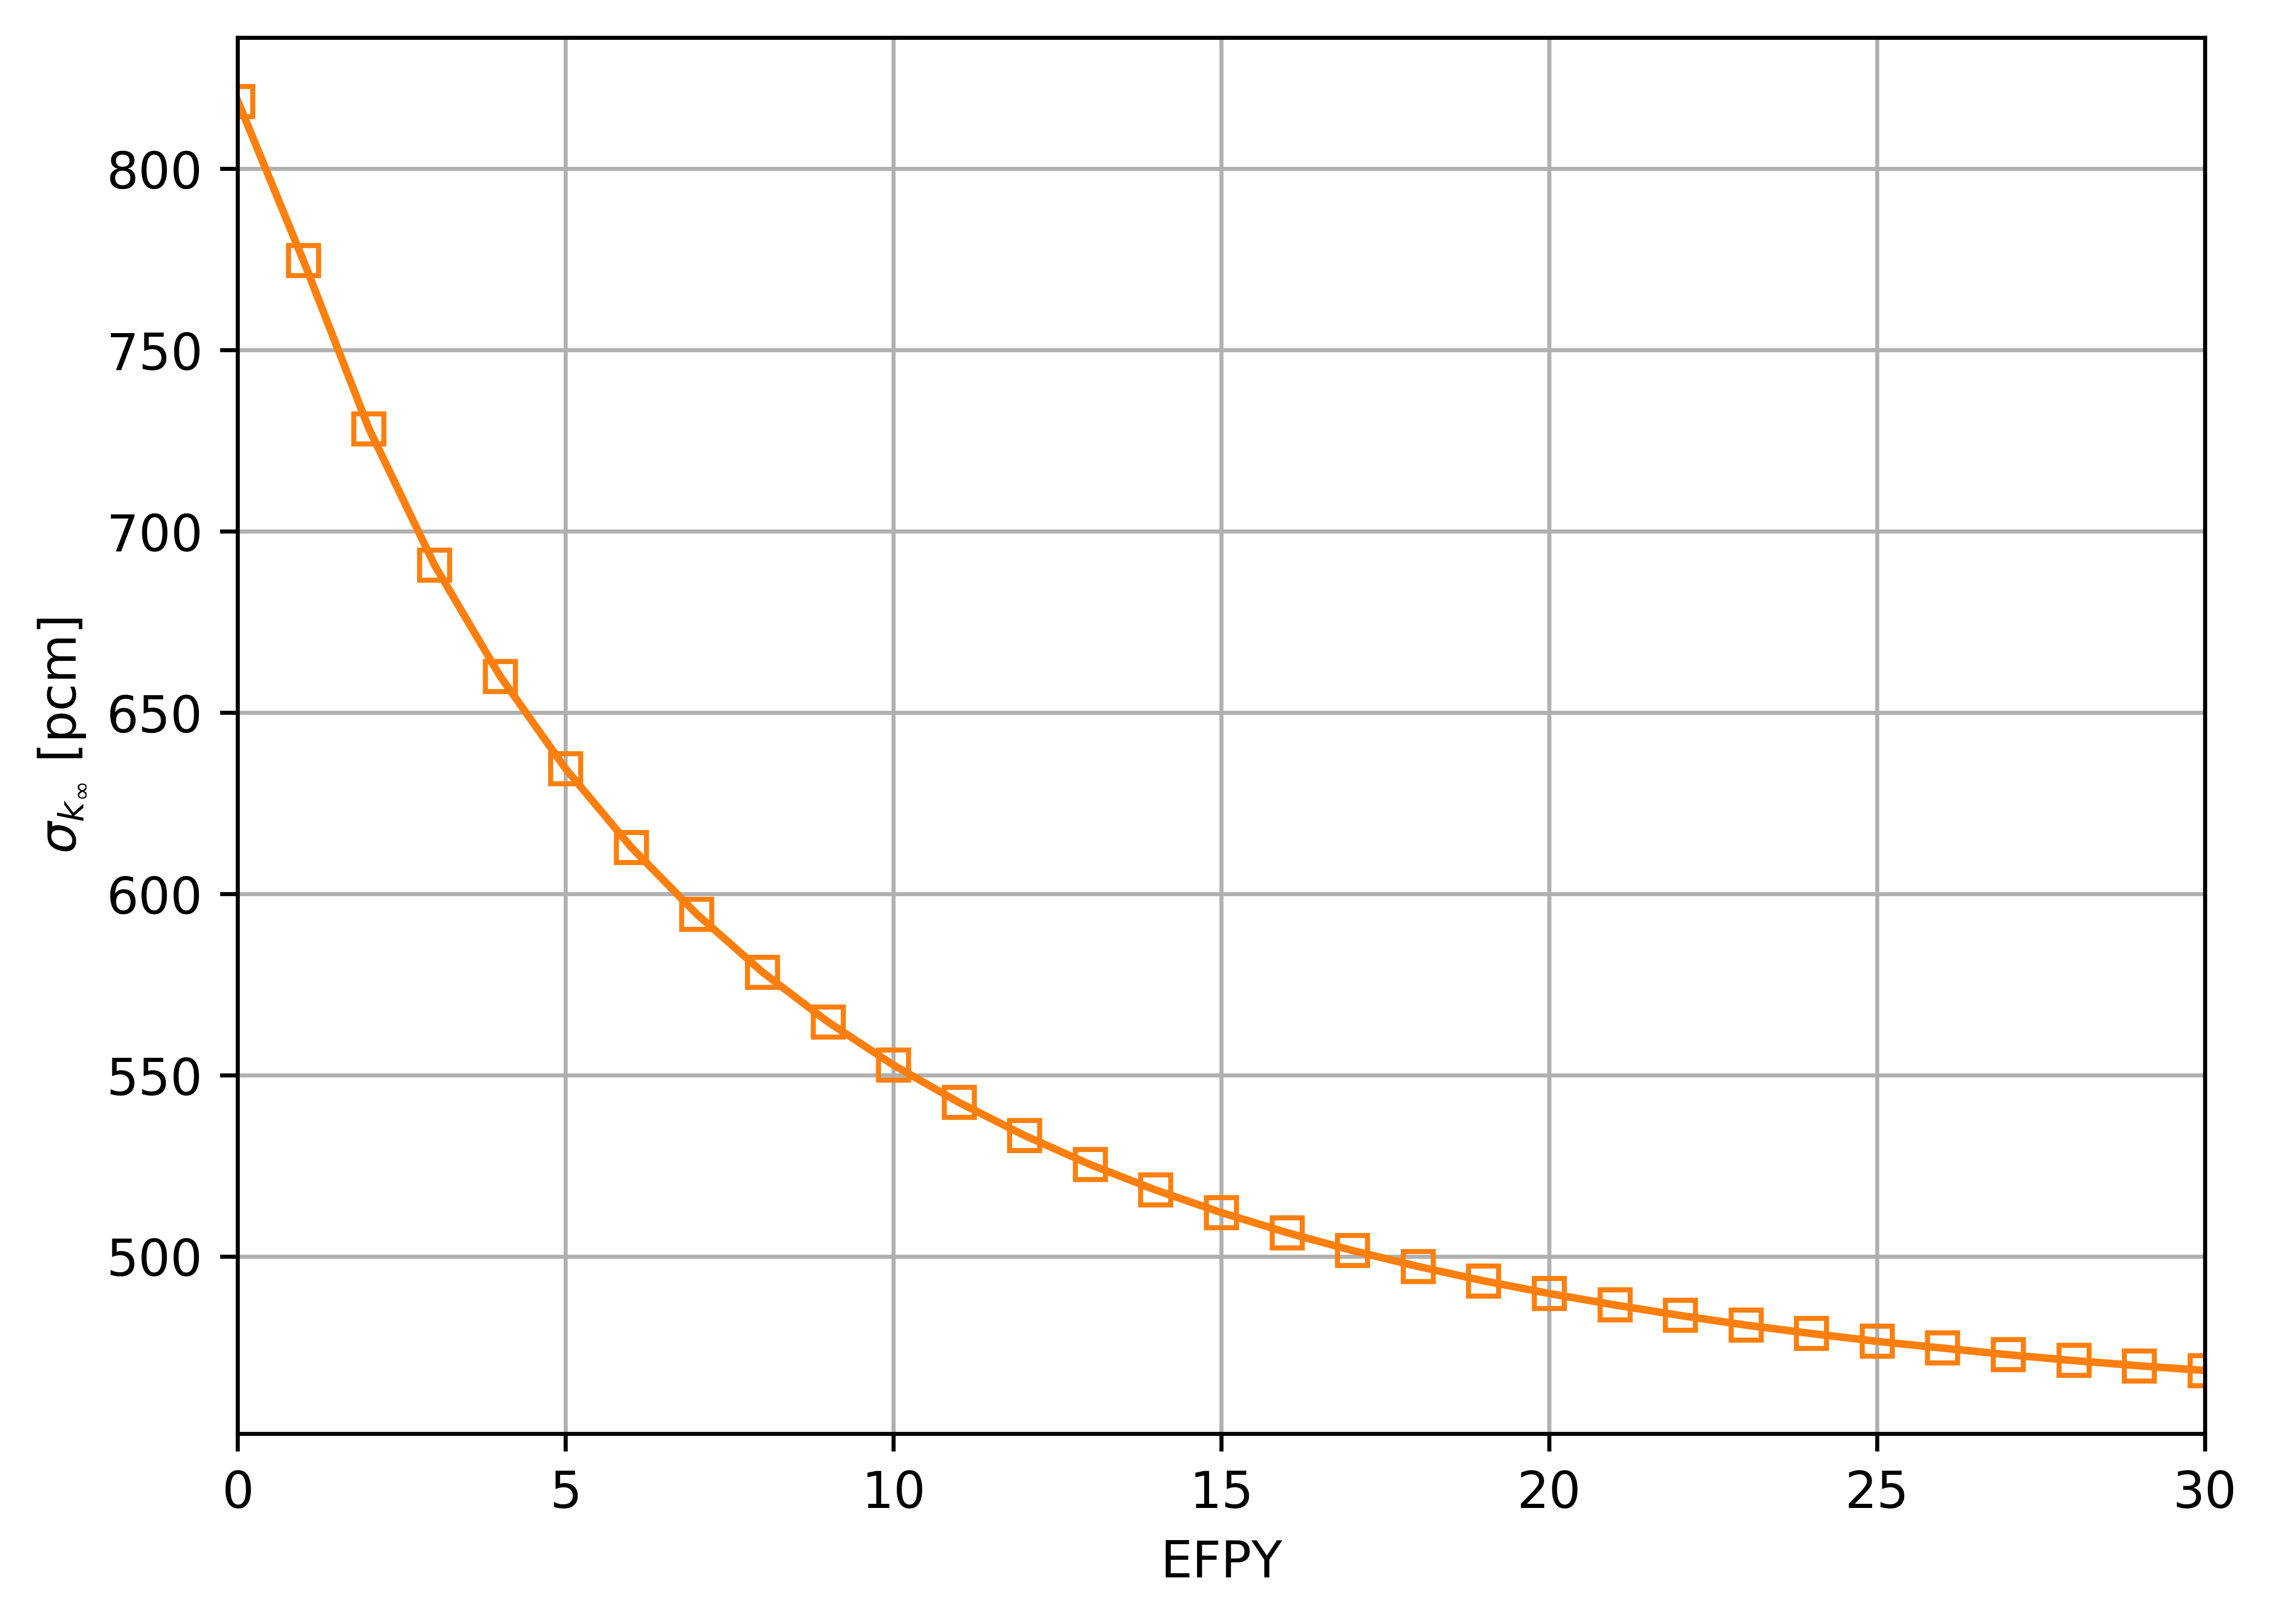
\includegraphics[width=\textwidth]{uq/scale_kinf_dynamics_for_tap.png}
	\caption{Calculated uncertainty in the infinite multiplication factor due 
		to the nuclear data uncertainty as a function of depletion time.}
	\label{fig:uq-scale-kinf}
\end{figure}

Figure~\ref{fig:uq-scale-kinf} demonstrates nuclear data-related uncertainty 
in the $k_{\infty}$ evolution during 30 years of operation. The $k_{\infty}$  
uncertainty decreased slowly because the $k_{\infty}$ mean value reduces over 
time from 1.01714 to 0.78143 due to fuel burnup. Considering more specific 
nuclear data contributions, at the \gls{BOL} the $k_{\infty}$ uncertainty is 
most likely to come from the fissile $^{235}$U fission ($n,f$) and neutron 
capture $(n,\gamma$) reaction cross sections; the $^{238}$U $(n,\gamma$) 
reaction cross section; and the elastic scattering cross section of hydrogen 
in zirconium hydride. However, moving toward the \gls{EOL}, the contributions 
to uncertainty from $^{235}$U data are expected to diminish due to the burnup 
and be substituted by the cross section uncertainties of the fissile plutonium 
(e.g., $^{239}$Pu, $^{241}$Pu). Notably, the $^{235}$U fission cross section 
uncertainty in intermediate and fast spectrum ranges (the \gls{TAP} is an
intermediate spectrum reactor, see Figure~\ref{fig:ben-spectrum-bol}) reaches 
up to 4\%, while it is less than 2.6\% for $^{239}$Pu and $^{241}$Pu. 
$^{239}$Pu and $^{241}$Pu capture and fission cross sections formed the 
dominant source of uncertainty after $^{235}$U was mostly depleted. 
%This $k_{\infty}$ 
%uncertainty evolution is in good agreement with results in the literature  
%\cite{rochman_nuclear_2014, radaideh_advanced_2019}. 

Moreover, the $k_{\infty}$ relative uncertainty from nuclear data slipped 
from 0.78\% at the \gls{BOL} to 0.46\% at the \gls{EOL}. This error is 
slightly larger than results in the literature for conventional \glspl{LWR} 
(e.g., 0.44\% \cite{williams_statistical_2013} or 0.55\% 
\cite{campolina_uncertainty_2018} for a \gls{PWR}). This discrepancy between 
$k_{\infty}$ uncertainty for the \gls{TAP} \gls{MSR} and \gls{PWR} likely 
originates with the $^{19}$F and $^{7}$Li nuclear data, which have significant 
covariances across reactions.

Figure~\ref{fig:uq-scale-u-pu} shows the standard deviations in uranium and 
plutonium isotopic inventory as a function of time. The uncertainty in 
$^{238}$U is minimal ($<0.1$\%) and almost constant with burnup because 
$^{238}$U mass does not change significantly from its initial inventory. The 
$^{236}$U uncertainty also is nearly constant during 30 years of operation and 
has a value of $\approx3.8$\%. However, $^{235}$U mass uncertainty increases 
steadily with burnup, due to its inventory decrease during 30 years of 
operation. The absolute mass uncertainty for $^{235}$U demonstrated growth 
from 5 kg at 1 year after startup to approximately 30 kg at the \gls{EOL}.

The uncertainty of major plutonium isotopes (e.g., $^{239}$Pu, $^{240}$Pu, 
$^{241}$Pu) is below 2\% over 30 years of burnup 
(Figure~\ref{fig:uq-scale-u-pu}, lower plot). The fissile $^{239}$Pu and 
poisonous $^{240}$Pu relative standard deviations are increased slightly from 
1.25\% to 1.6\% and from 1.65\% to 1.95\%, respectively. The relative standard 
deviation in fissile $^{241}$Pu mass is significant at the beginning of the 
operation, when its inventory is small (4 kg), and then decreases and 
approaches an equilibrium value of $\approx1.45$\% at the \gls{EOL}. The 
most significant relative standard deviation is observed for $^{242}$Pu mass 
($8.13$\%) because its concentration in fuel is minimal throughout 30 years 
of operation (Table~\ref{tab:uq-scale-mean-std-rsd}).
\begin{figure}[hbp!] % replace 't' with 'b' to 
	\centering
	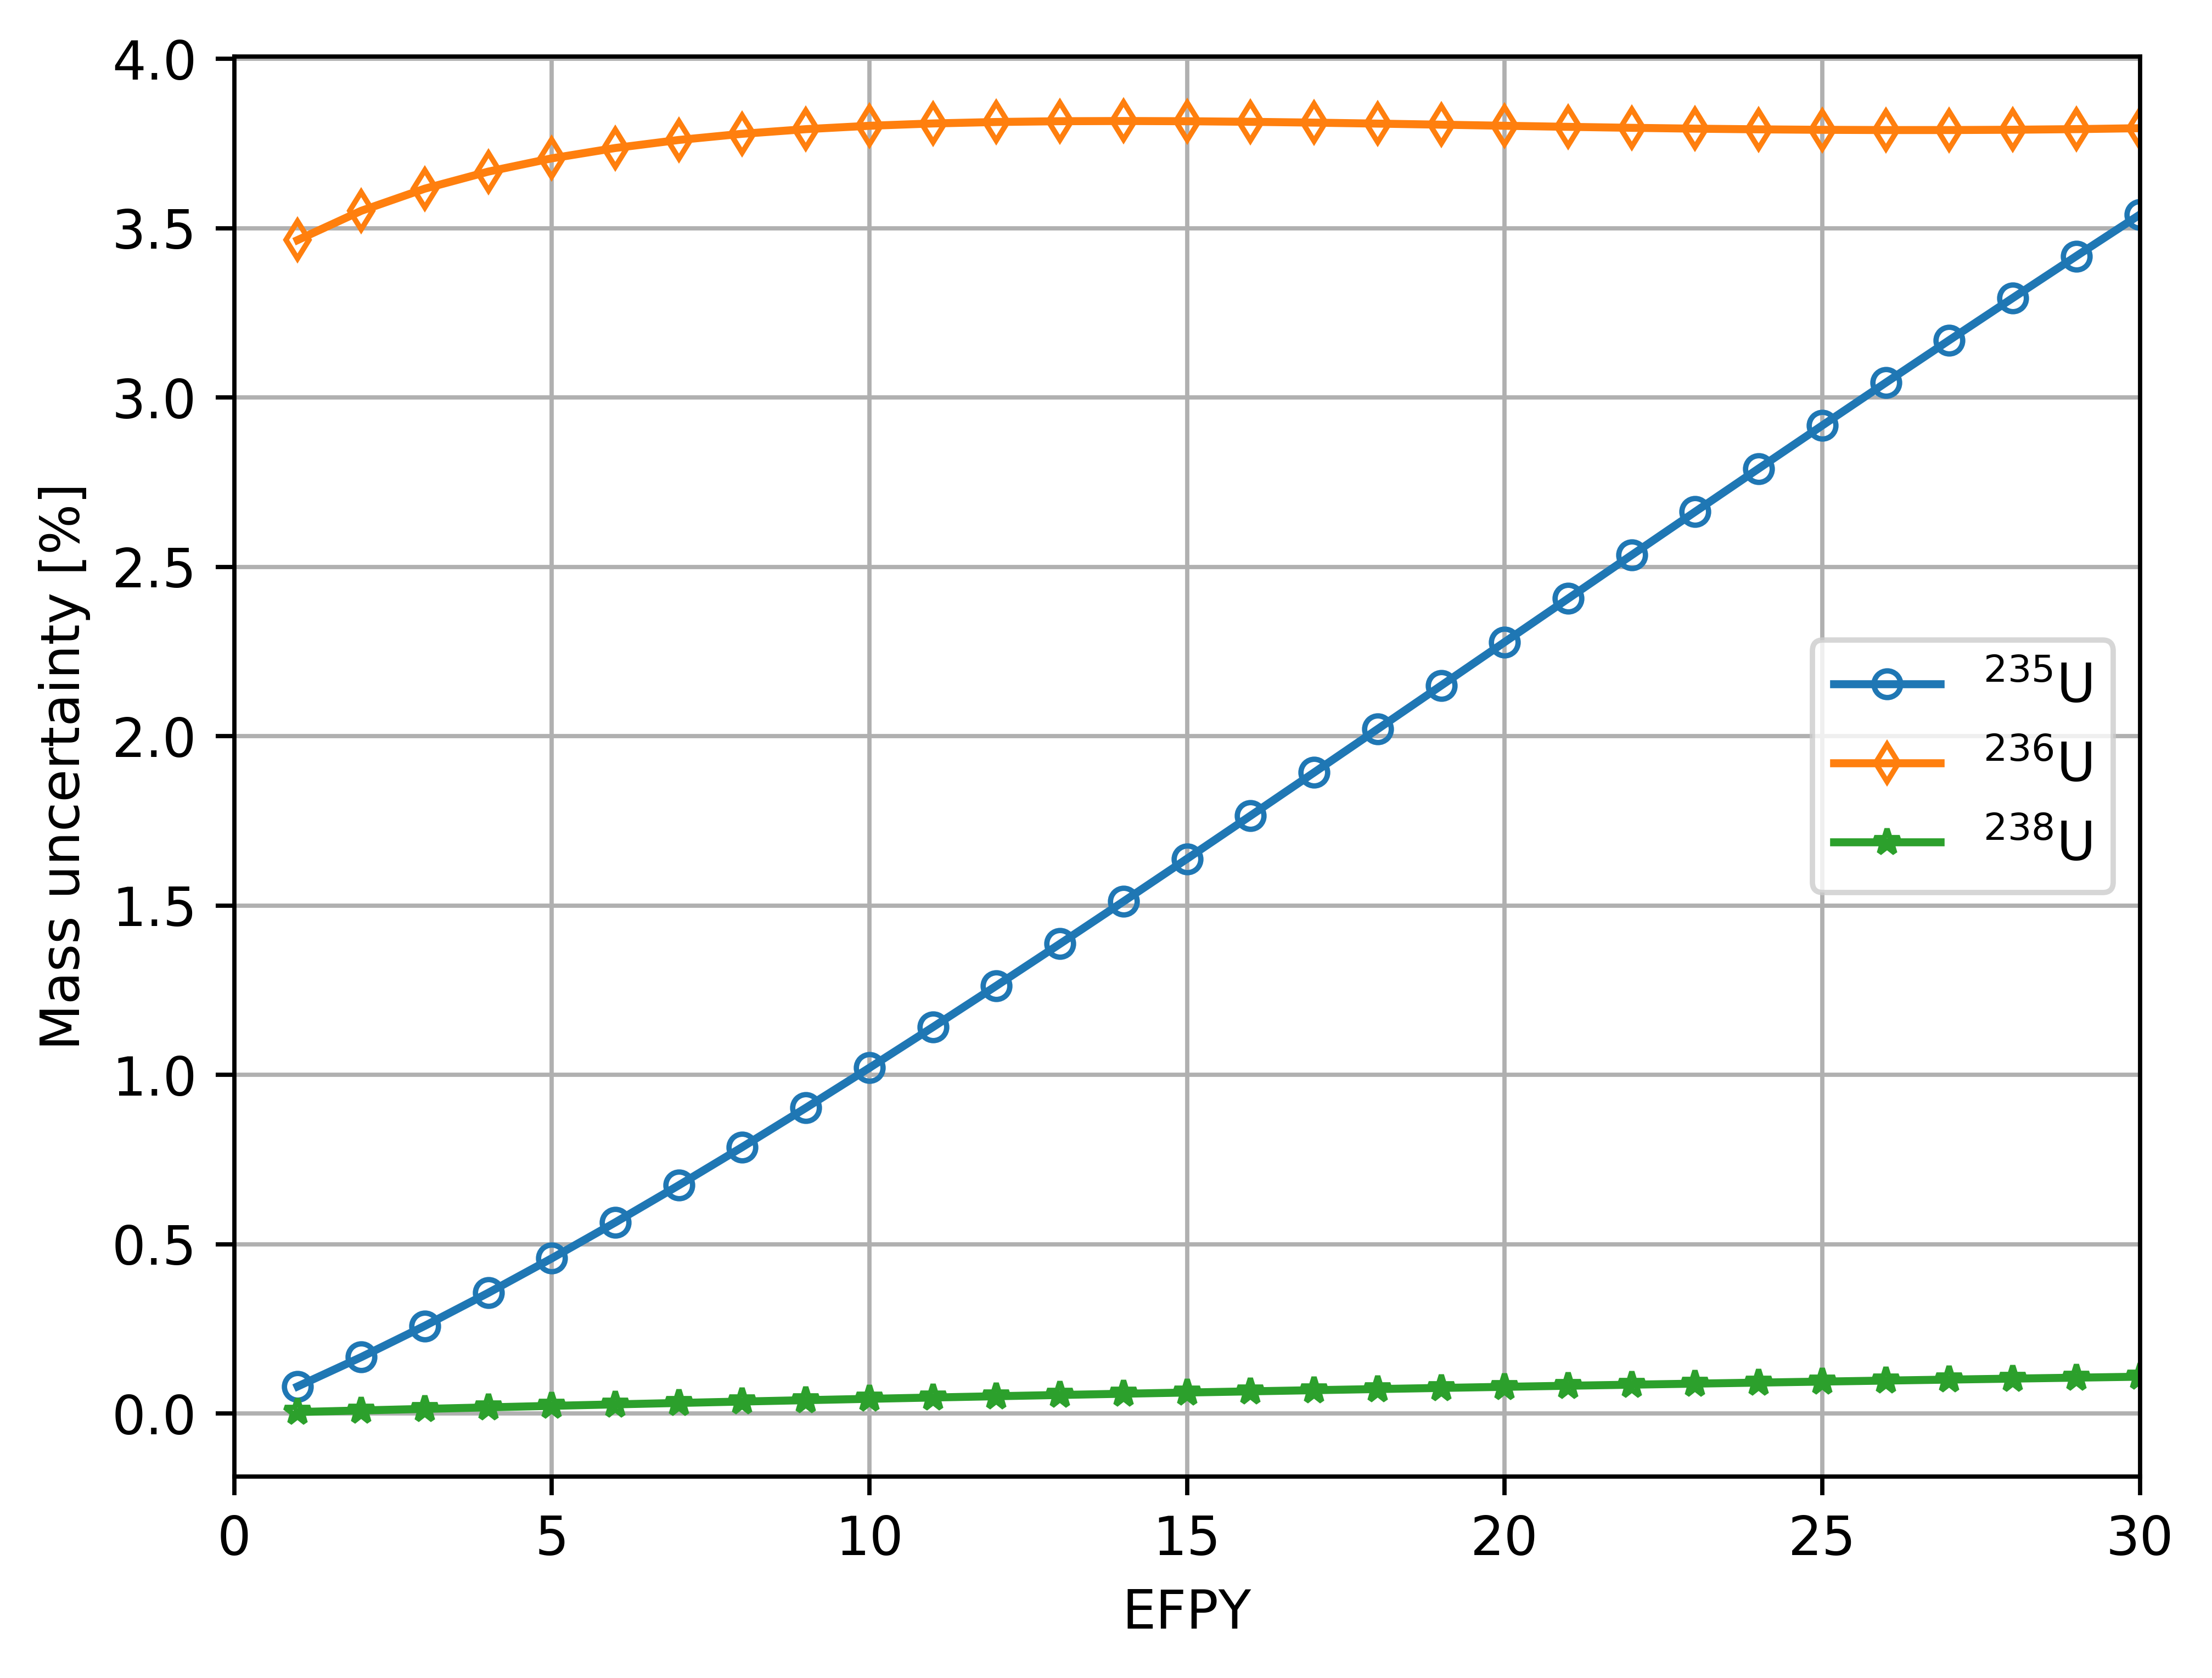
\includegraphics[width=0.85\textwidth]{uq/scale_mass_std_u.png}
	\vspace{-12mm}
	\hspace{0.0mm}
	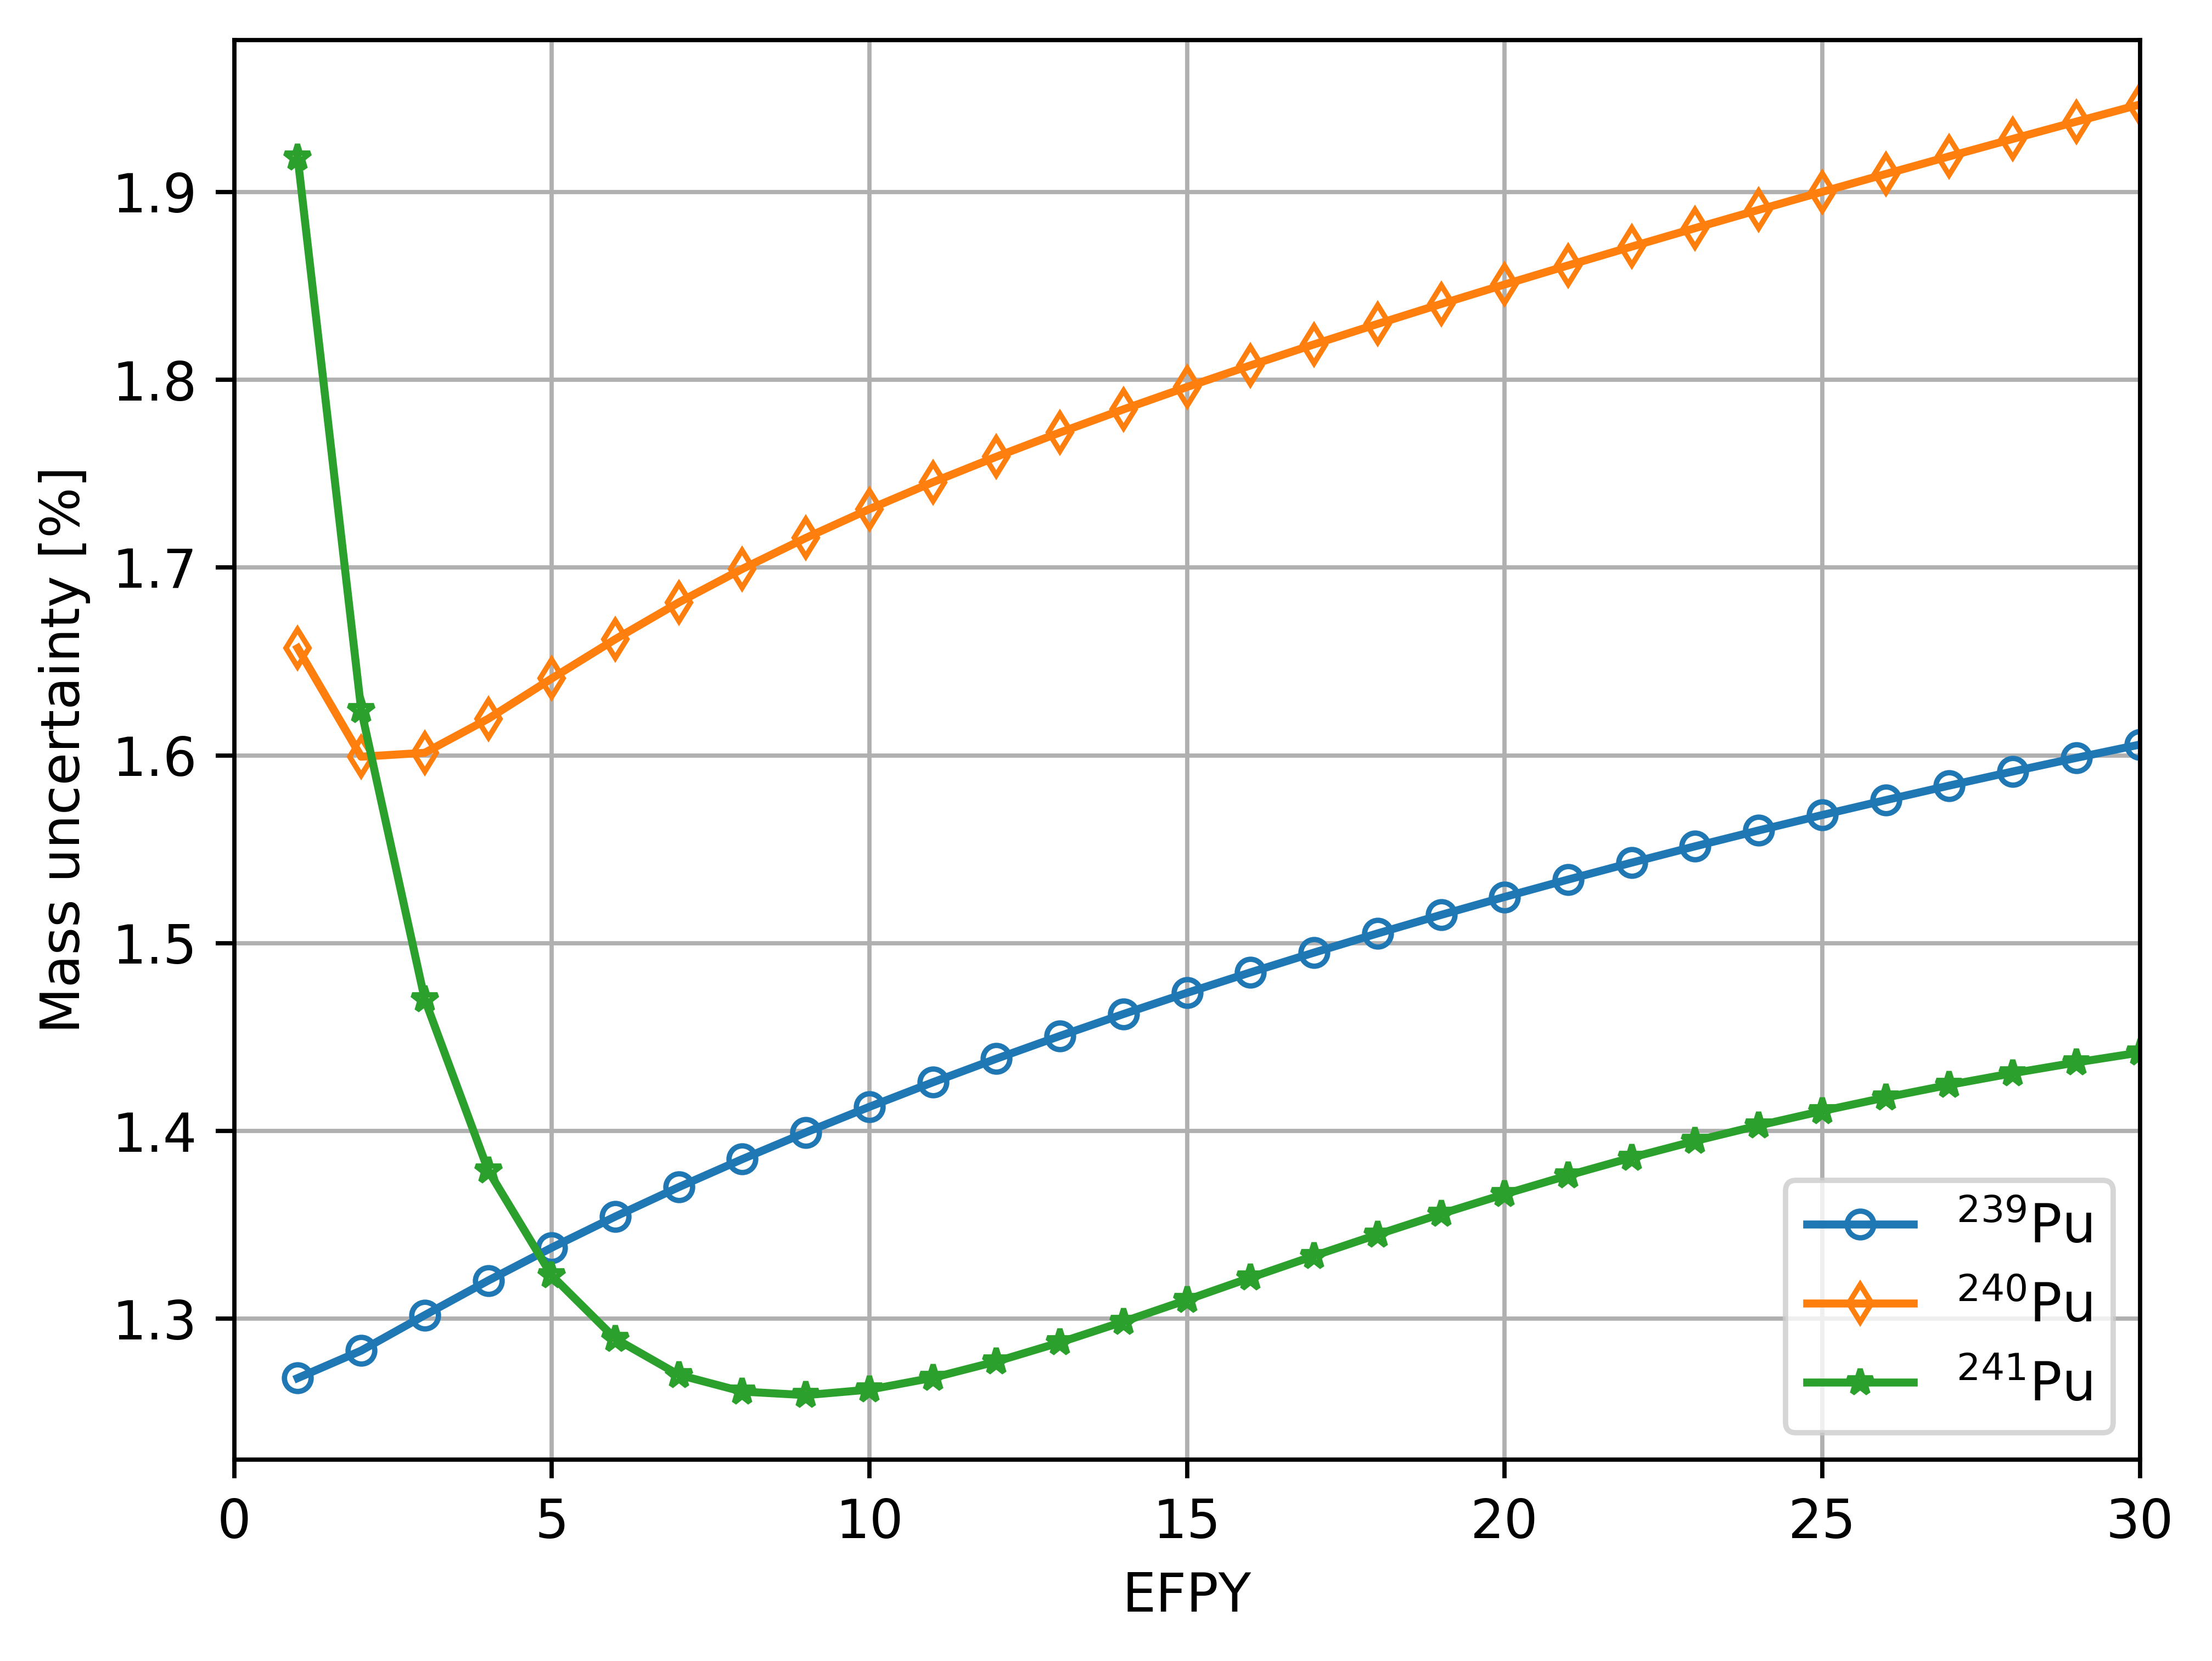
\includegraphics[width=0.85\textwidth]{uq/scale_mass_std_pu.png}
	\vspace{+8mm}
	\caption{Nuclear data-related uncertainty evolution in the uranium (upper) 
		and plutonium (lower) isotopic inventory during 30 years of depletion.}
	\label{fig:uq-scale-u-pu}
\end{figure}

Figure~\ref{fig:uq-scale-xe-i} shows the mass uncertainties for the selected 
\glspl{FP}: $^{135}$Xe and its primary direct precursor, $^{135}$I. The masses 
of $^{135}$Xe and $^{135}$I are in the ranges of 24-27 g and 18-19 g, 
respectively. As expected, relative standard deviations for these isotopes are 
relatively low due to minimal uncertainty of fission yield for $^{235}$U. The 
relative standard deviation of $^{135}$Xe mass changes in a range from 
0.47\% to 0.6\%, while the $^{135}$I standard deviation ranges from 0.35\% to 
0.56\%.
\begin{figure}[hbp!] % replace 't' with 'b' to 
	\centering
	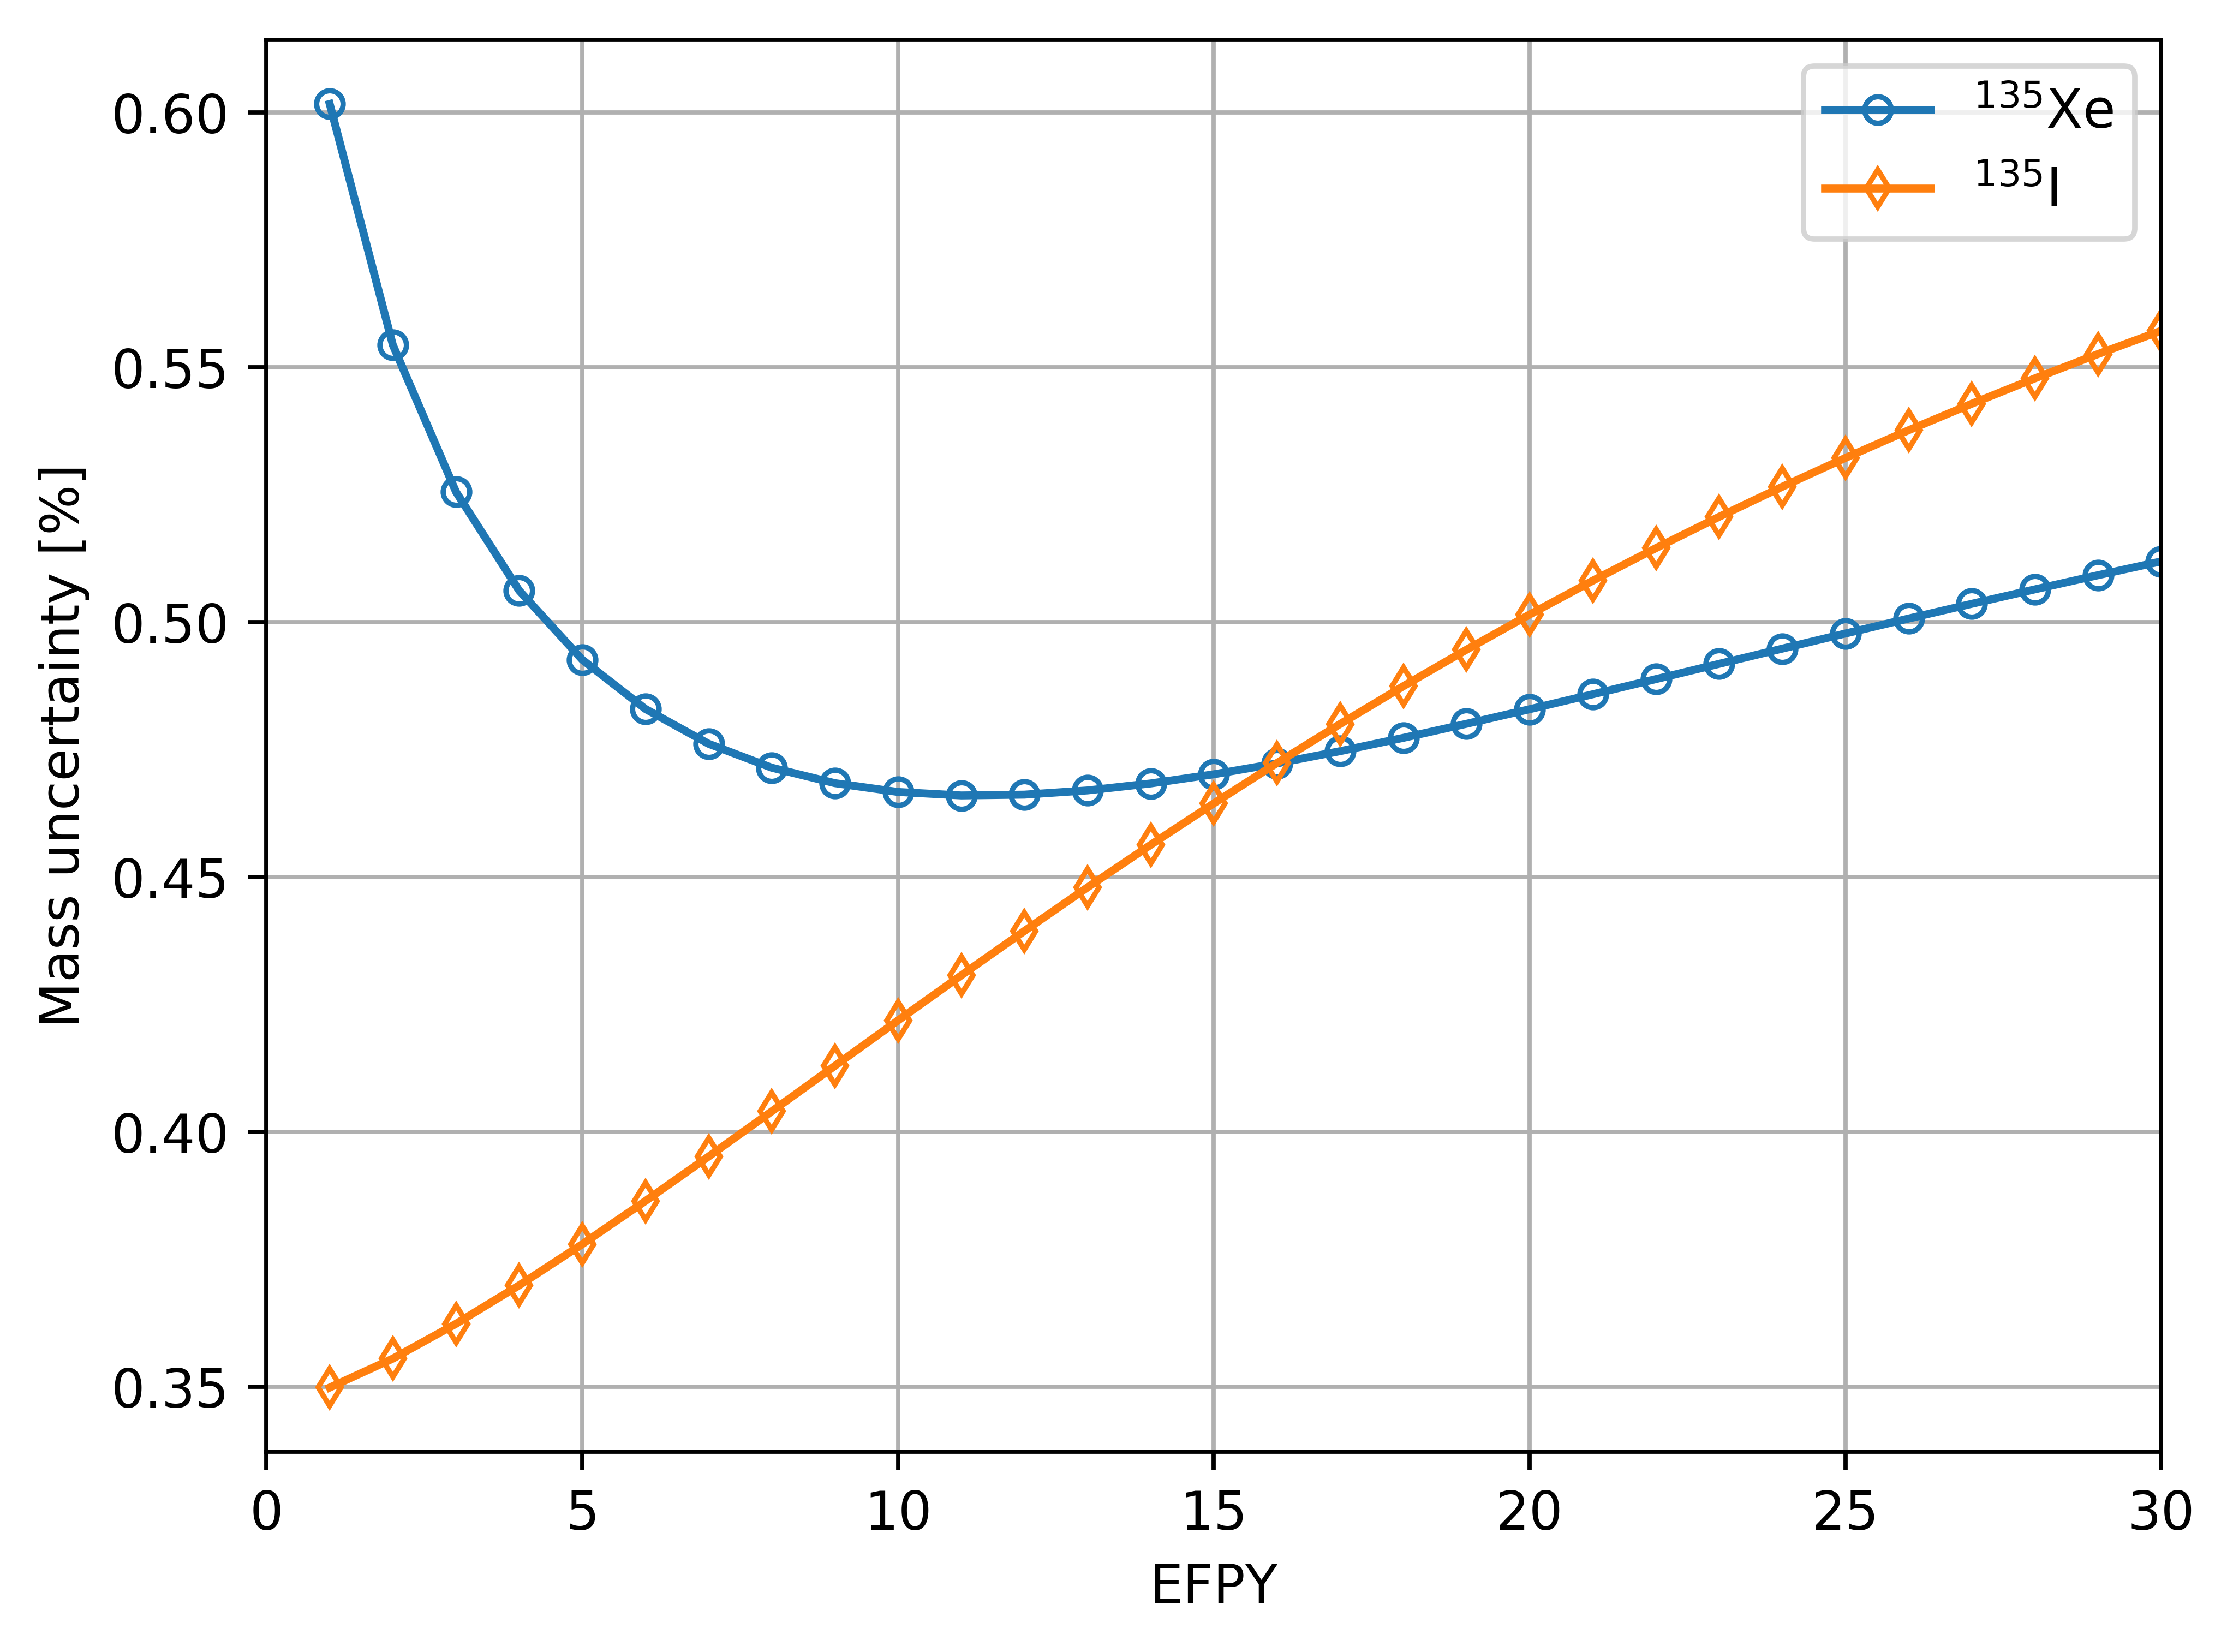
\includegraphics[width=0.85\textwidth]{uq/scale_mass_std_xe_i.png}
	\caption{Nuclear data-related uncertainty evolution in $^{135}$Xe and 
		$^{135}$I isotopic inventory during 30 years of depletion.}
	\label{fig:uq-scale-xe-i}
\end{figure}

Table~\ref{tab:uq-scale-mean-std-rsd} summarizes the nuclear data-related 
uncertainty in the isotopic inventory for the \gls{TAP} \gls{MSR} after 30 
years of operation. Overall, the mass uncertainties due to nuclear data 
uncertainties are two orders of magnitude larger than uncertainty due to 
the statistical error in \gls{MC}.  

All results presented in this section are based on 800 random samples obtained 
using the Sampler tool in SCALE. Figure~\ref{fig:uq-scale-convergence} 
shows the convergence of $k_{\infty}$ and $^{235}$U mass uncertainty with 
number of random samples. Notably, after 500 samples the $k_{\infty}$ and 
$^{235}$U mass uncertainties stabilize. Overall, 500 random samples is 
enough to accurately estimate uncertainty in the isotopic inventory due to 
uncertainty in nuclear data. 

%%%%%%%%%%%%%%%%%%%%%%%%%%%%%%%%%%%%%%%%
\begin{table}[hbp!]
	\centering
	\caption{Mean value, Standard Deviation (STD), and Relative Standard 
		Deviation (RSD) of mass for the major isotopes after 30-year depletion 
		analysis for the \gls{TAP} reactor. Only nuclear data-related 
		uncertainty is considered.}
	\begin{tabularx}{0.7\textwidth}{L R R R R}
		\hline
		\textbf{Isotope}  & \textbf{Mean [kg]} & \textbf{STD [kg]} & 
		\textbf{RSD [\%]}\\ \hline
		$^{234}$U  & 21.6  & 0.75  & 3.48\% \\
		$^{235}$U  & 839.4 & 29.72 & 3.54\% \\
		$^{236}$U  & 1154.9& 43.83 & 3.79\% \\
		$^{238}$U  & 112,206.1 & 122.32 & 0.11\% \\
		$^{238}$Pu & 335.56& 11.05 & 3.29\% \\
		$^{239}$Pu & 5558.1& 89.25 & 1.61\% \\
		$^{240}$Pu & 1594.6& 31.04 & 1.95\% \\
		$^{241}$Pu & 639.1 & 9.21  & 1.44\% \\
		$^{242}$Pu & 164.0 & 13.33 & 8.13\% \\
		$^{241}$Am & 204.9 & 6.15  & 3.00\% \\
		$^{135}$Xe & 0.03  &$<0.01$& 0.51\% \\
		$^{135}$I  & 0.02  &$<0.01$& 0.56\% \\ \hline
	\end{tabularx}
	\label{tab:uq-scale-mean-std-rsd}
	\vspace{-0.9em}
\end{table}
%%%%%%%%%%%%%%%%%%%%%%%%%%%%%%%%%%%%%%%%%%%%%%%%%%%%%%%%%%%%%%%%%%%%%%%%%%%%%%%


\begin{figure}[hbp!] % replace 't' with 'b' to 
	\centering
	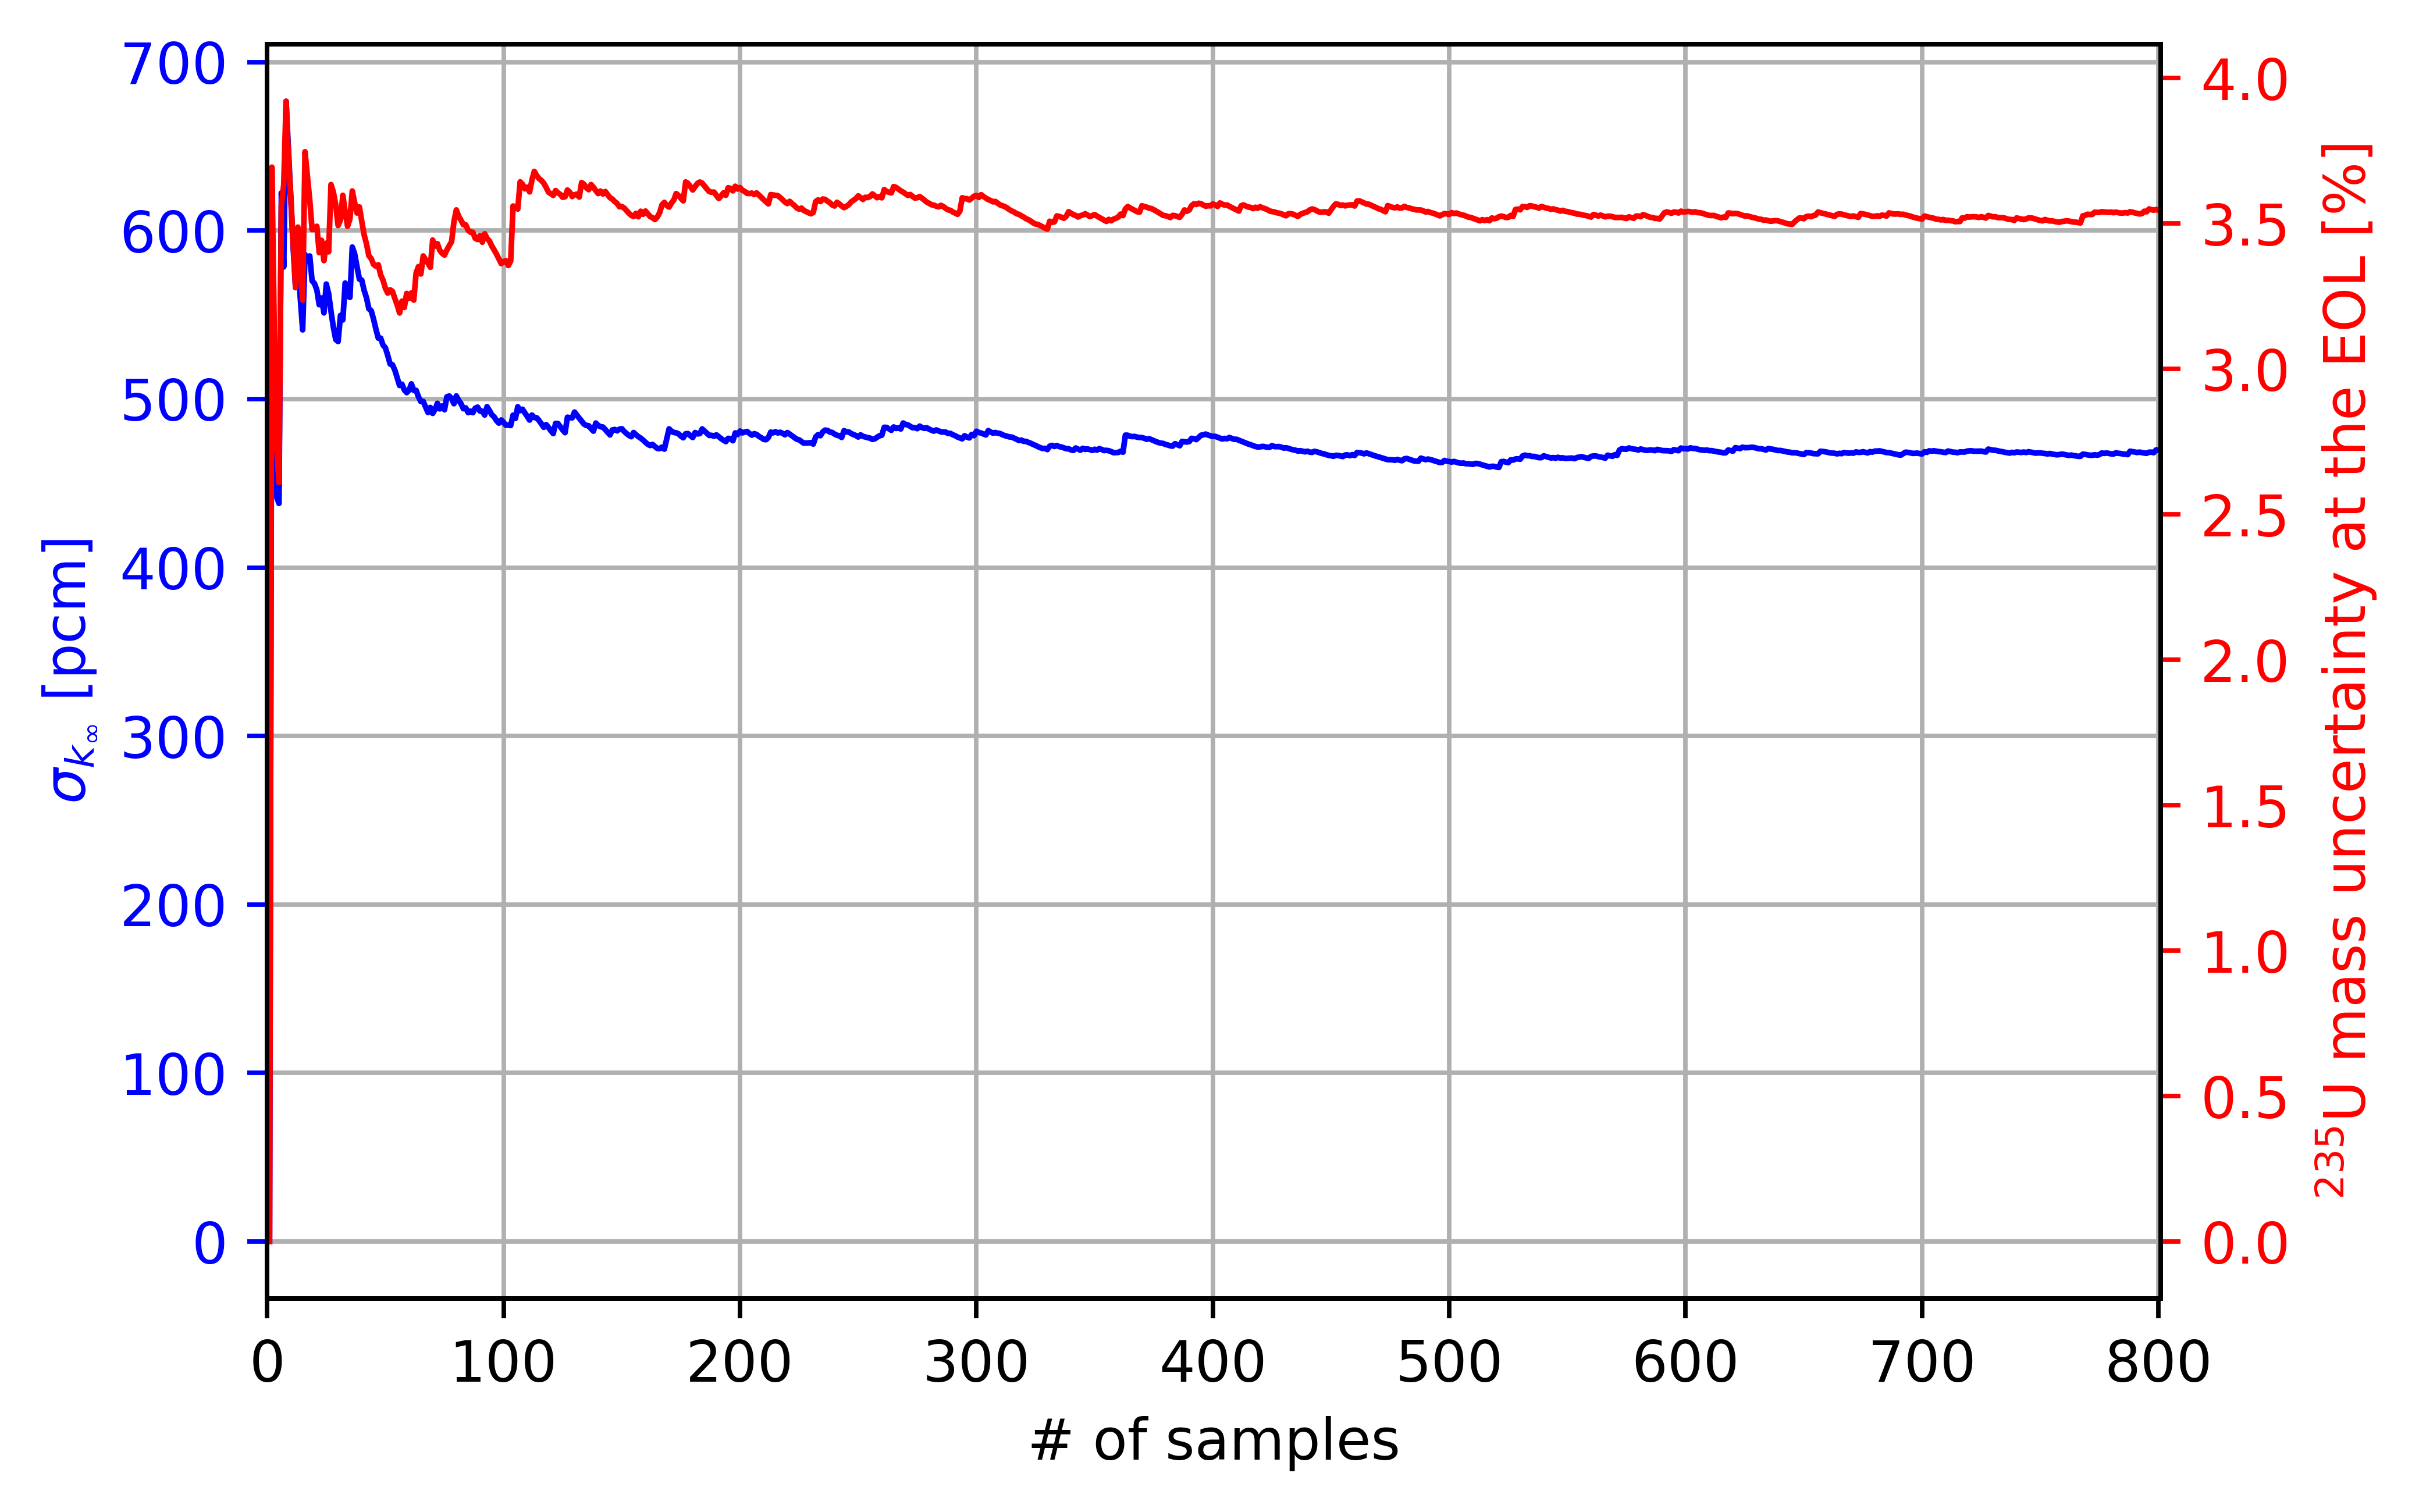
\includegraphics[width=\textwidth]{uq/scale_convergance_for_tap.png}
	\caption{Convergence of $k_{\infty}$ and $^{235}$U mass uncertainties due 
		to the nuclear data uncertainty as a function of the number of samples 
		for 
		simulation using SCALE with the Sampler module.}
	\label{fig:uq-scale-convergence}
\end{figure}

\section{Concluding remarks}
Uncertainty propagation analysis was performed for the depletion calculation 
for the \gls{TAP} \gls{MSR} 30-year burnup. I separately considered two 
primary sources of uncertainty in the depletion calculations: stochastic 
uncertainty in the neutron flux distribution and uncertainty in the nuclear 
data. Stochastic error in the isotopic composition was obtained using the 
Serpent Continuous Energy Monte Carlo code by running the same depletion 
sequence 1000 times, each time with a new initial random seed. The 
Sampler module in SCALE 6.2 with a 56-group covariance library was used to 
obtain nuclear data-related uncertainty in the isotopic composition of the 
fuel salt. 
Uncertainties in the input nuclear data (cross sections, fission yields, decay 
constants) are propagated throughout all steps of the transport/depletion 
sequence, including self-shielding, space-energy flux calculation, and isotope 
transmutation. 

The stochastic errors in isotopic masses are below 0.067\% 
for 7.5 million neutron histories (total neutron flux relative stochastic 
error $<0.01$\%). Therefore, it is unnecessary to consider the accumulation of 
the stochastic error for the fuel depletion in the \gls{TAP} reactor 
considered in this dissertation.
Finally, the stochastic error in the isotopic inventory could be reduced to 
almost zero by increasing the number of neutron histories, but it is 
impractical due to the sublinear convergence rate of the Monte Carlo method 
($O(\sqrt{N})$).

On the other hand, the computed errors in the isotopic inventory due to the 
nuclear data uncertainties are a few orders of magnitude larger and cannot 
be ignored. The nuclear data-related errors are in the range from 1\% to 2\% 
for the masses of $^{239}$Pu, $^{240}$Pu, and $^{241}$Pu, and about 3-8\% for  
$^{234}$U, $^{235}$U, $^{236}$U, $^{238}$Pu, $^{242}$Pu, and $^{241}$Am. 
Finally, the mass uncertainty for the selected \glspl{FP} ($^{135}$Xe and 
$^{135}$I), which are the subject of interest of the current work, is below 
0.6\%. Overall, the principal source of uncertainty in depletion calculations 
arises from to the nuclear data covariances.

Finally, this chapter demonstrated that the standard deviation in the 
multiplication factor due to the nuclear data uncertainty ranges from 804 to 
469 $pcm$, while the stochastic error is only about 30 $pcm$. Overall, to 
accurately capture the isotopic inventory evolution for the \gls{TAP} concept 
using SaltProc v1.0 with Serpent Monte Carlo code, it is unnecessary to 
waste a vast computational power to simulate $10^7-10^9$ neutron histories per 
each depletion step because the impact of the stochastic errors in 
neutron fluxes is negligible compared with the nuclear data-related errors.
\section{Methodology}
\subsection{Fuel salt reprocessing system}

\begin{frame}
  \frametitle{Fuel salt reprocessing system overview: gas separation}
  Gaseous fission products (e.g., Xe, Kr) must be removed from the fuel salt 
  to avoid reactor poisoning ($\sigma_{a,^{135}Xe}=10^6\dots10^7$b). 
  
      \begin{columns}
      	\column[t]{4.0cm}
    \begin{block}{Noble gas removal}
      \begin{enumerate}
      	\item[\textcolor{blue}{\textbullet}] bubble generator injects He 
      	bubbles in the salt stream
      	\item[\textcolor{green}{\textbullet}] noble gases migrate to the He 
      	bubbles 
      	\item[\textcolor{red}{\textbullet}] gas separator discharges the 
      	poison-rich bubbles
      \end{enumerate}
    \end{block}    	
      	
     	\column[t]{8cm}
  \begin{figure}[t]
	  \centering
	  		\vspace{-4mm}
		\includegraphics[width=1.03\textwidth]{./images/msbr_gas_separation.pdf}
	\caption{Schematic flow diagram of the \gls{MSBR} gas separation system 
	(figure reproduced from Robertson \emph{et al.}  
	\cite{robertson_conceptual_1971}).} 
    \end{figure}

	\end{columns}
\end{frame}

\begin{frame}
  \frametitle{Mathematical model for gas separation efficiency}
  		\vspace{-1mm}
Xenon removal efficiency ($\epsilon_{Xe}$) in a gas separation system is 
\cite{peebles_removal_1968, sada_gas-liquid_1987}:
\begin{align}
& \qquad\qquad \epsilon_{Xe} = \frac{1-e^{-\beta}}{1+\alpha} \nonumber \\
\alpha &= \frac{RTQ_{L}}{HQ_{G}} \nonumber \\
\beta &= K_L \frac{6}{d_b} \frac{Q_G}{Q_G+G_L} \frac{A_C L (1+\alpha)}{Q_{L}} 
\nonumber \\
Q_{L}&= \mbox{volumetric salt flow rate [$m^3/s$]} \nonumber \\
Q_{G}&= \mbox{volumetric helium flow rate [$m^3/s$]} \nonumber \\
H &= \mbox{Henry's law constant [$Pa\cdot mol^{-1}\cdot L$]} \nonumber \\
d_b &= \mbox{helium bubble diameter [m]} \nonumber \\
K_L &= \mbox{liquid phase mass transfer coefficient [m/s].} \nonumber
\end{align}
		\vspace{-5mm}
  \begin{figure}[t]
	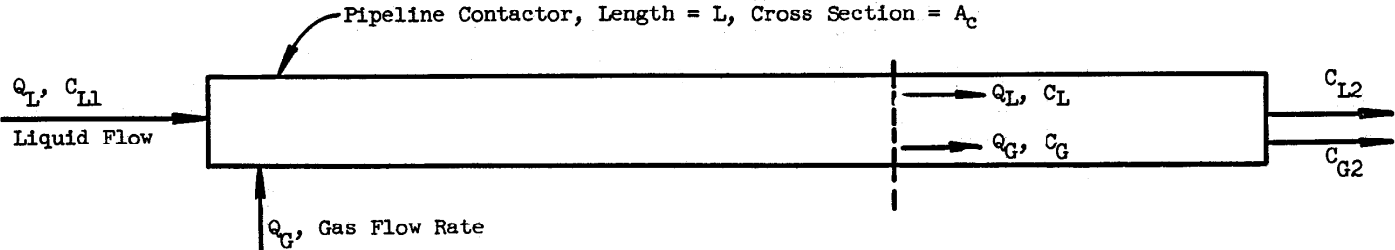
\includegraphics[width=0.77\textwidth]{./images/pipeline_contactor.png}
	\vspace{-2mm}
	\caption{Flow diagram for gas separator (figure reproduced from Peebles 
		\emph{et al.} \cite{peebles_removal_1968}).}
\end{figure}

\end{frame}


\begin{frame}
\frametitle{Fuel processing system overview: TAP concept}
\begin{textblock*}{12.4cm}(0.25cm,1.7cm) % {block width} (coords)
\begin{figure}[htp!] % replace 't' with 'b' to 
	\begin{columns}
		\column{0.65\linewidth}
			\hspace{+3mm}
		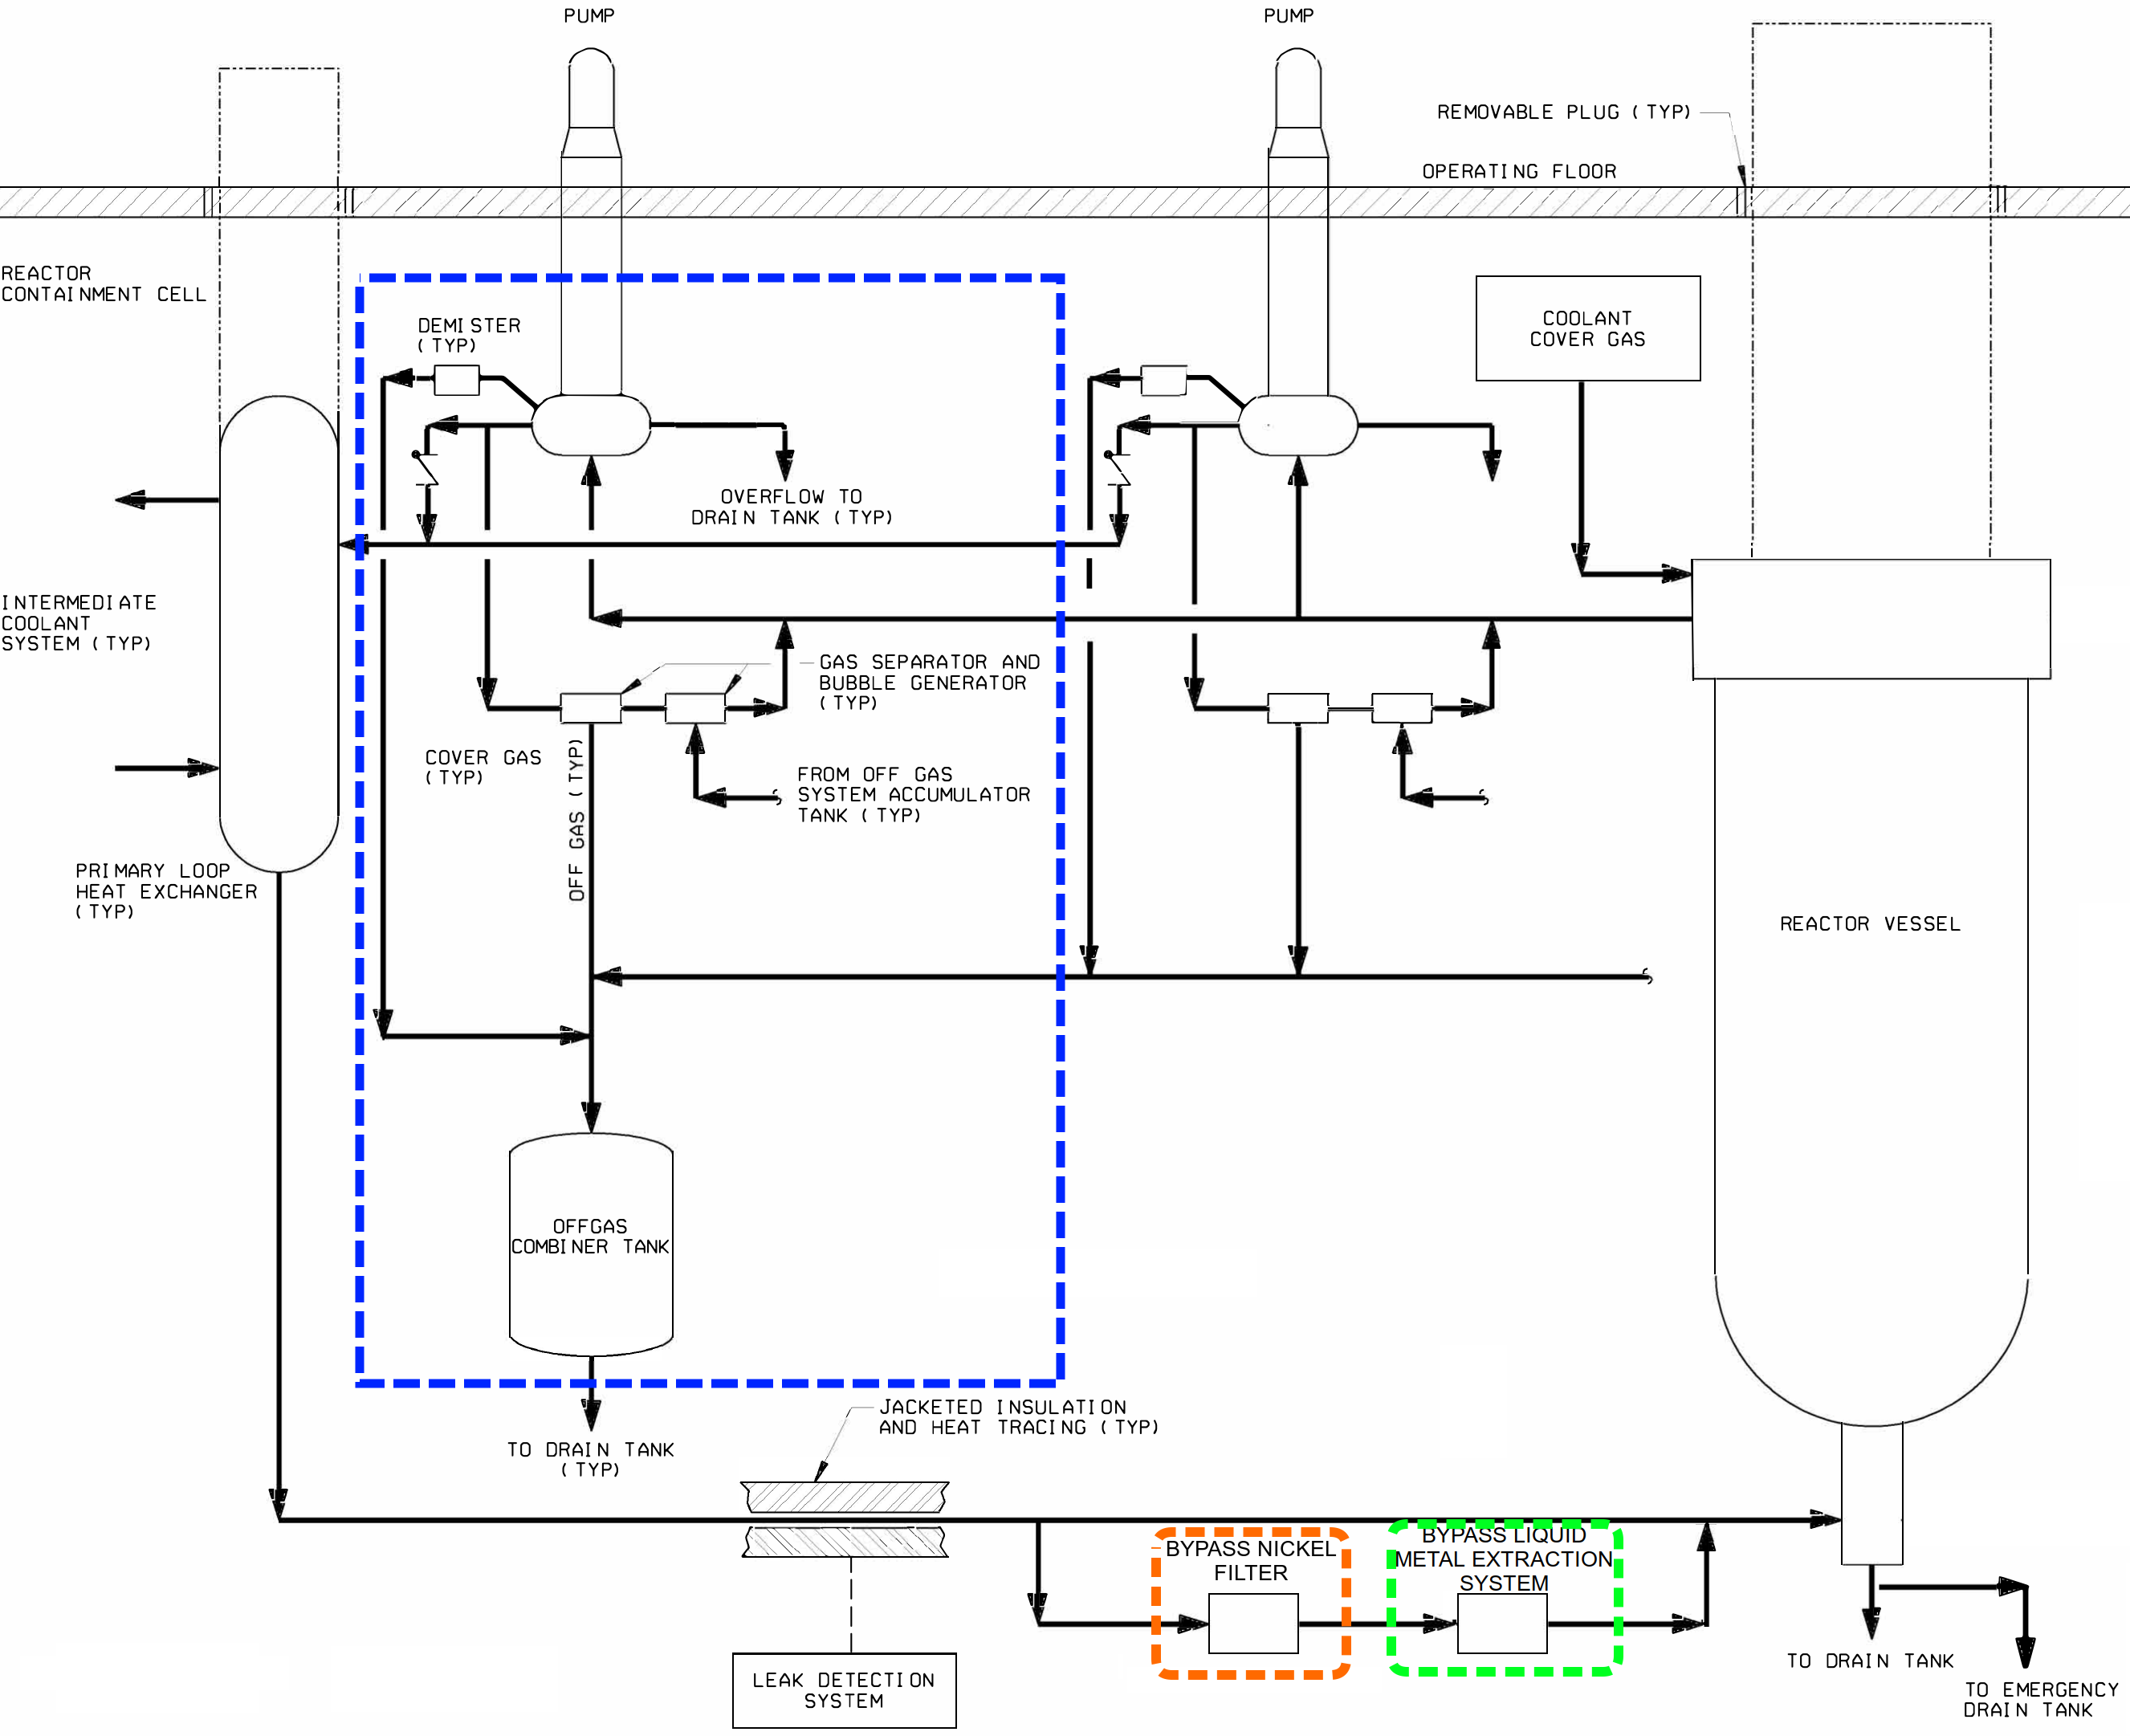
\includegraphics[height=0.88\textheight]{../dissertation/figures/ch4/tap_primary_loop.png}
		
		\column{0.3\linewidth}
		\caption{Simplified \gls{TAP} primary loop design including off-gas 
		system 
		(blue), nickel filter (orange) and liquid metal extraction system 
		(green) \cite{transatomic_power_transatomic_2019}.}
	\end{columns}
\end{figure}
\end{textblock*}
\end{frame}


\subsection{SaltProc tool design}


\begin{frame}
\frametitle{SaltProc class architecture}
	\begin{itemize}
		\item \textit{Simulation} class
			\begin{itemize}
				\item Manages simulation process
				\item Stores data into the HDF5 database
				\item Tracks time, power level
			\end{itemize}
		\item \textit{Depcode} class
			\begin{itemize}
				\item Contains attributes and methods for reading user's input
				\item Creates input files for depletion code
				\item Parses depletion code output 
			\end{itemize}
		\item \textit{Process} class
			\begin{itemize}
				\item Represents fuel processing system component
				\item Contains attributes of the component ($\vec{\epsilon}$, 
				throughput rate)
				\item Tracks waste stream
			\end{itemize}
		\item \textit{MaterialFlow} class
			\begin{itemize}
				\item Instances of that class represents the material flowing between processes
			\end{itemize}
	\end{itemize}
		\vspace{1mm}
	\begin{figure}[ht!] % replace 't' with 'b' to 
		\centering
		\begin{overprint}
		\onslide<1>\centerline{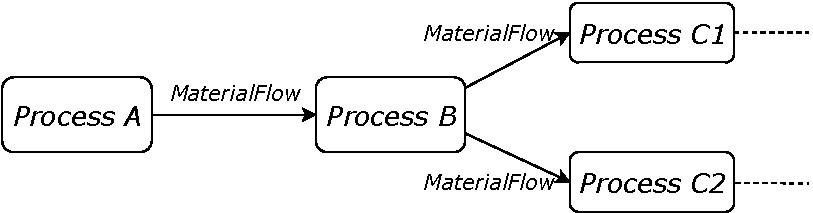
\includegraphics[width=0.6\textwidth]{../dissertation/figures/ch2/materialflow.pdf}}
		\onslide<2>\centerline{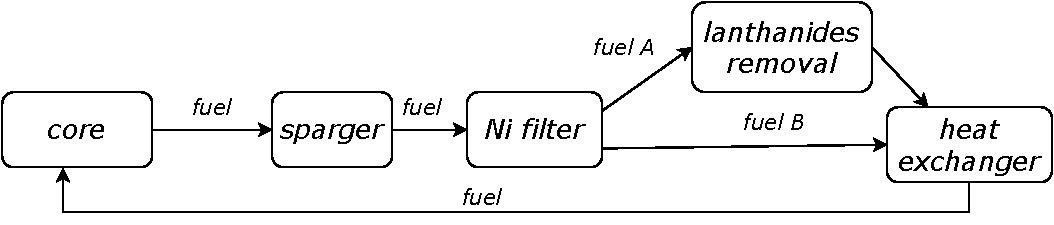
\includegraphics[width=0.6\textwidth]{../dissertation/figures/ch2/tap_materialflow.pdf}}
		\end{overprint}
		\vspace{-2mm}
		\caption{Schematic for passing material data between fuel processing 
		system components.}
	\end{figure}

\end{frame}


\begin{frame}
\frametitle{SaltProc flowchart}
\begin{textblock*}{12.4cm}(0.07cm,1.7cm) % {block width} (coords)
\begin{figure}[ht!] % replace 't' with 'b' to \centering
	\centering
	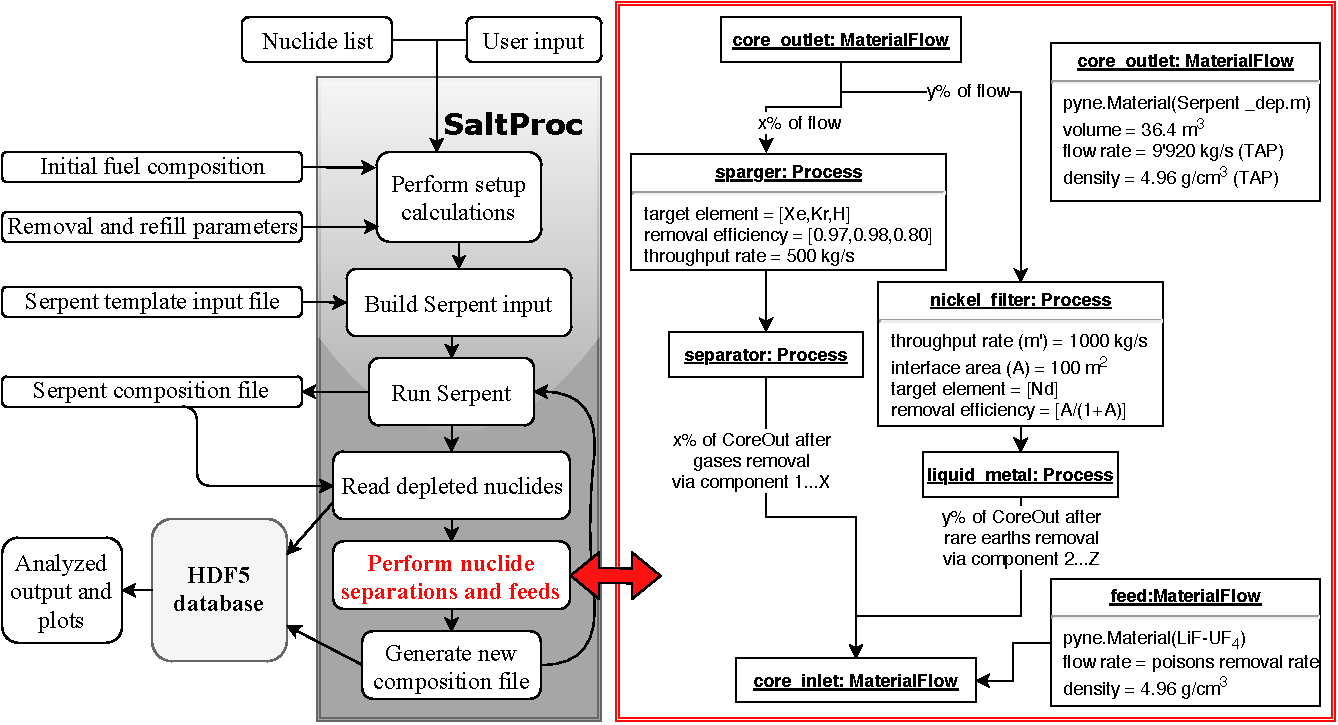
\includegraphics[width=\textwidth]{../dissertation/figures/ch2/saltproc_flowchart.pdf}
		\vspace{-4mm}
	\caption{SaltProc v1.0 Python package flowchart with example of object 
	instances.}
\end{figure}
\end{textblock*}

\end{frame}


\begin{frame}
\frametitle{Multi-component fuel reprocessing system model in SaltProc}       

\begin{figure}[htp!] % replace 't' with 'b' to 
	\centering
	\vspace{-2mm}
	\begin{overprint}
	\onslide<1>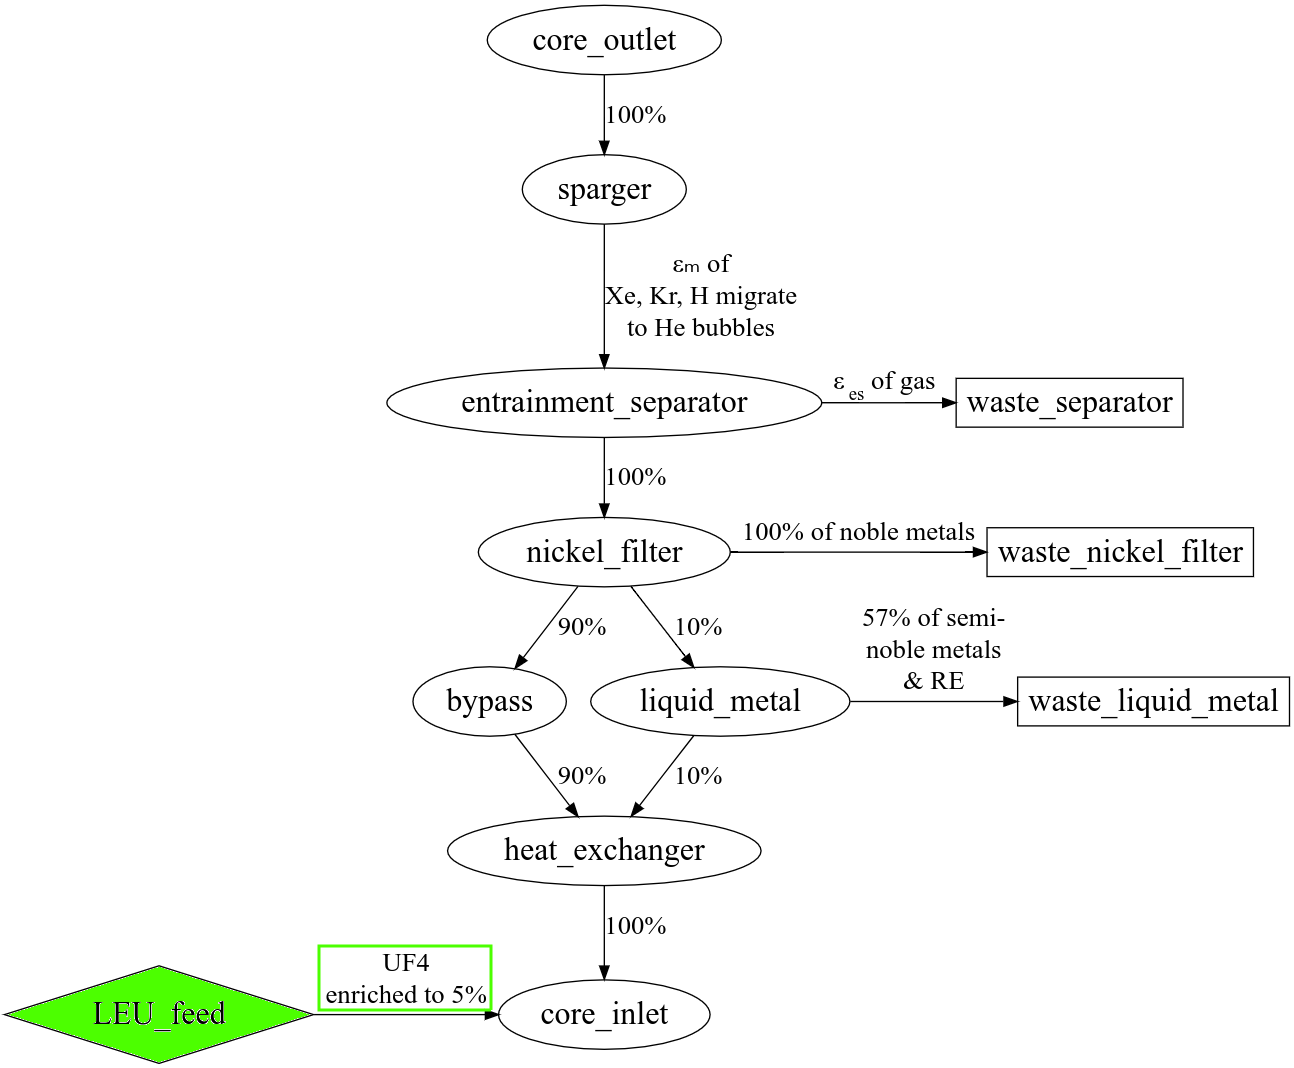
\includegraphics[height=0.85\textheight]{./images/tap_saltproc_var_eps.png}
		\vspace{-2mm}
    \caption{\textcolor{cyan}{\gls{TAP}} reprocessing scheme for 
	SaltProc demonstration.}
	\onslide<2>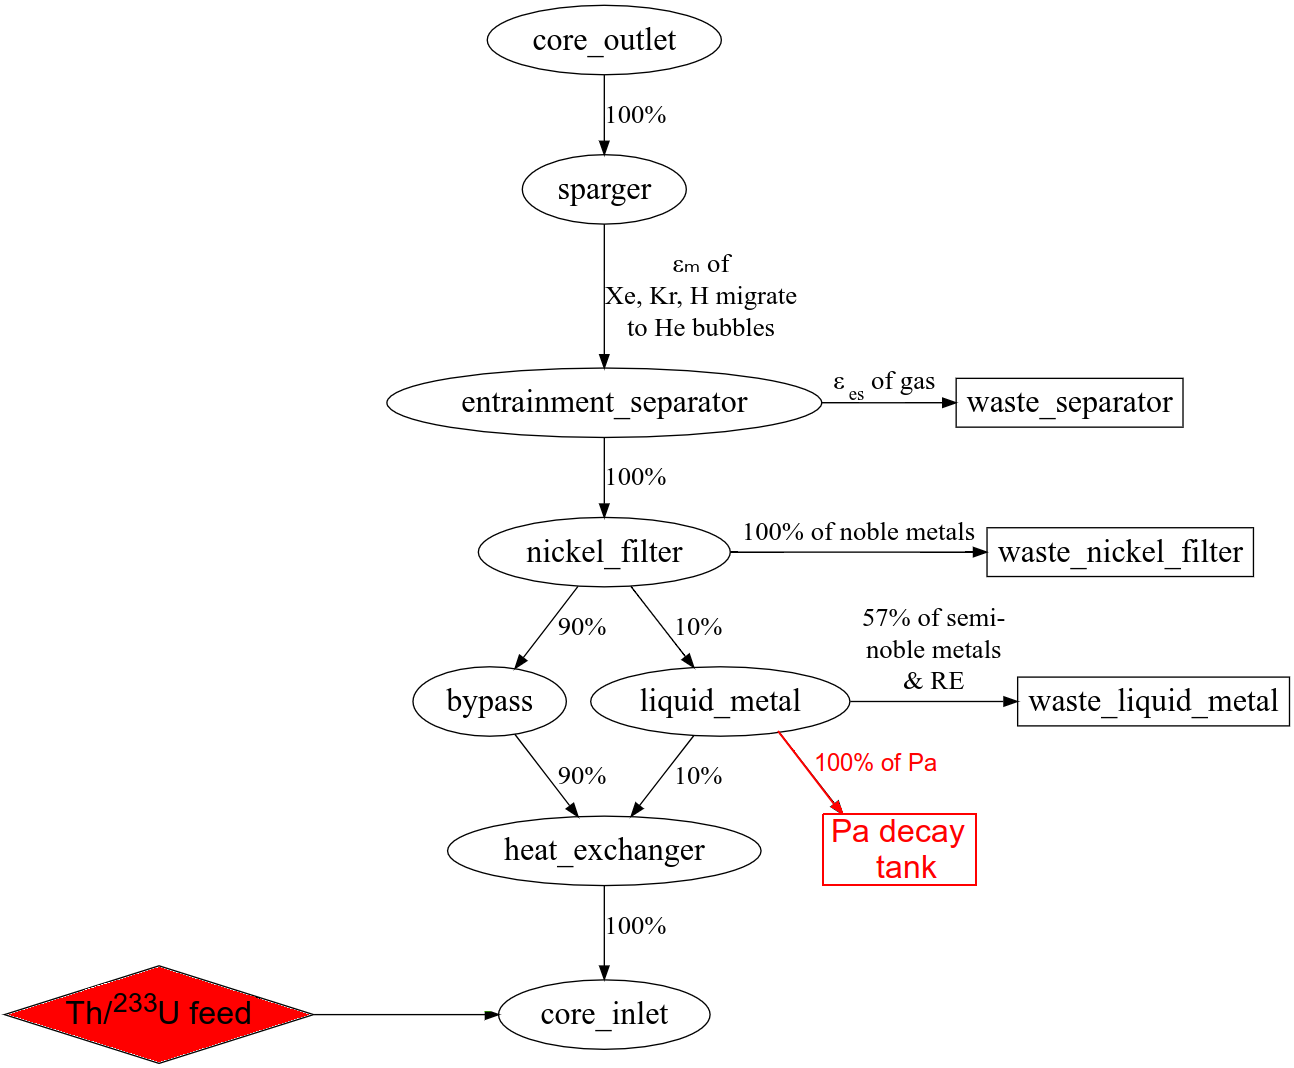
\includegraphics[height=0.85\textheight]{./images/msbr_saltproc_var_eps.png}
		\vspace{-2mm}
	\caption{\textcolor{red}{\gls{MSBR}} reprocessing scheme for 
	SaltProc demonstration.}
	\end{overprint}
\end{figure}

\end{frame}


\begin{frame}[fragile]
\frametitle{DOT-code describing reprocessing system as a directed graph}
\small
\begin{verbatim}
digraph fuel {
==============================================================================
core_outlet -> sparger [label="100%"]
sparger -> waste_sparger [label="60% of Xe, Kr, H"]
sparger -> entrainment_separator [label="100%"]
entrainment_separator -> nickel_filter [label="100%"]
entrainment_separator -> waste_entrainment_separator [label="97% of Xe, Kr, H"]
nickel_filter -> bypass [label="90%"]
bypass -> heat_exchanger [label="90%"]
nickel_filter -> waste_nickel_filter [label="100% of noble metals"]
nickel_filter -> liquid_metal [label="10%"]
liquid_metal -> heat_exchanger [label="10%"]
liquid_metal -> waste_liquid_metal [label="57% of seminoble metals & RE"]
heat_exchanger -> core_inlet [label="100%"]
LEU_feed -> core_inlet
==============================================================================
# Optional parameters to prettify plots
\end{verbatim}
\end{frame}
\section{Results}
\subsection{Lifetime-long depletion: MSBR}

\begin{frame}
\frametitle{Molten Salt Breeder Reactor (MSBR) design}

\begin{textblock*}{12.5cm}(0.1cm,2.1cm) % {block width} (coords)
	
	\begin{columns}
		\column[t]{6cm}
		%%%%%%%%%%%%%%%%%%%%%%%%%%%%%%%%%%%%%%%%
		\begin{table}[h!]
			\fontsize{7}{9}\selectfont
			\caption{Summary of principal data for the \gls{MSBR} 
				\cite{robertson_conceptual_1971}. }
			\vspace{-2mm}
			\begin{tabularx}{\textwidth}{ p{3.6cm}  X}
				\hline
				Thermal power				           		& 2250 MW$_{th}$\\ 
				Electric power		                		& 1000 MW$_e$   
				\\  
				Net thermal efficiency        			    & 44.4\%       	
				\\  
				Salt volume fraction in Zone I				& 0.132			\\ 
				Salt volume fraction in Zone II  			& 0.37			\\ 
				Fuel salt inventory (Zone I)				& 8.2 m$^3$     \\
				Fuel salt inventory (Zone II)				& 10.8 m$^3$    \\
				Fuel salt inventory (annulus)				& 3.8 m$^3$     \\
				Fuel salt components    & LiF-BeF$_2$-ThF$_4$-\newline
				$^{233}$UF$_4$\\  
				Fuel salt composition           & 71.75-16-\newline 12-	
				0.25mole\%	\\  
				Neutron spectrum						    & thermal \\
				\hline
			\end{tabularx}
		\end{table}
		%%%%%%%%%%%%%%%%%%%%%%%%%%%%%%%%%%%%%%%%%%%%%%%%
		
		\column[t]{5.6cm}
		\vspace{-1mm}
		\begin{figure}      
			\hspace{-12mm}
			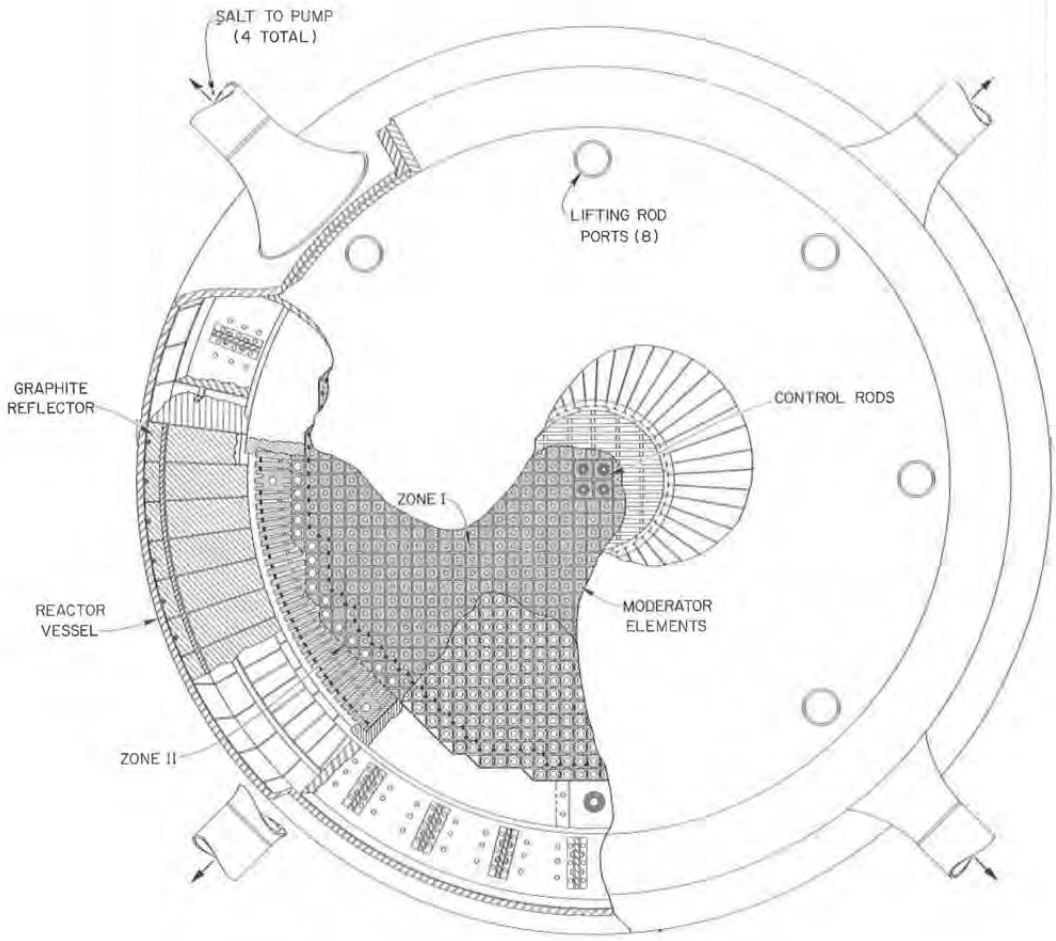
\includegraphics[height=1.05\textwidth]{./images/plan_view_vessel.png}
			\caption{Plan view of \gls{MSBR} vessel 
				\cite{robertson_conceptual_1971}.}
		\end{figure}
	\end{columns}
	
\end{textblock*}

\end{frame}


\begin{frame}
\frametitle{Geometry of MSBR model (Serpent)}

\begin{textblock*}{12.5cm}(0.1cm,1.9cm) % {block width} (coords)
\begin{figure}      
	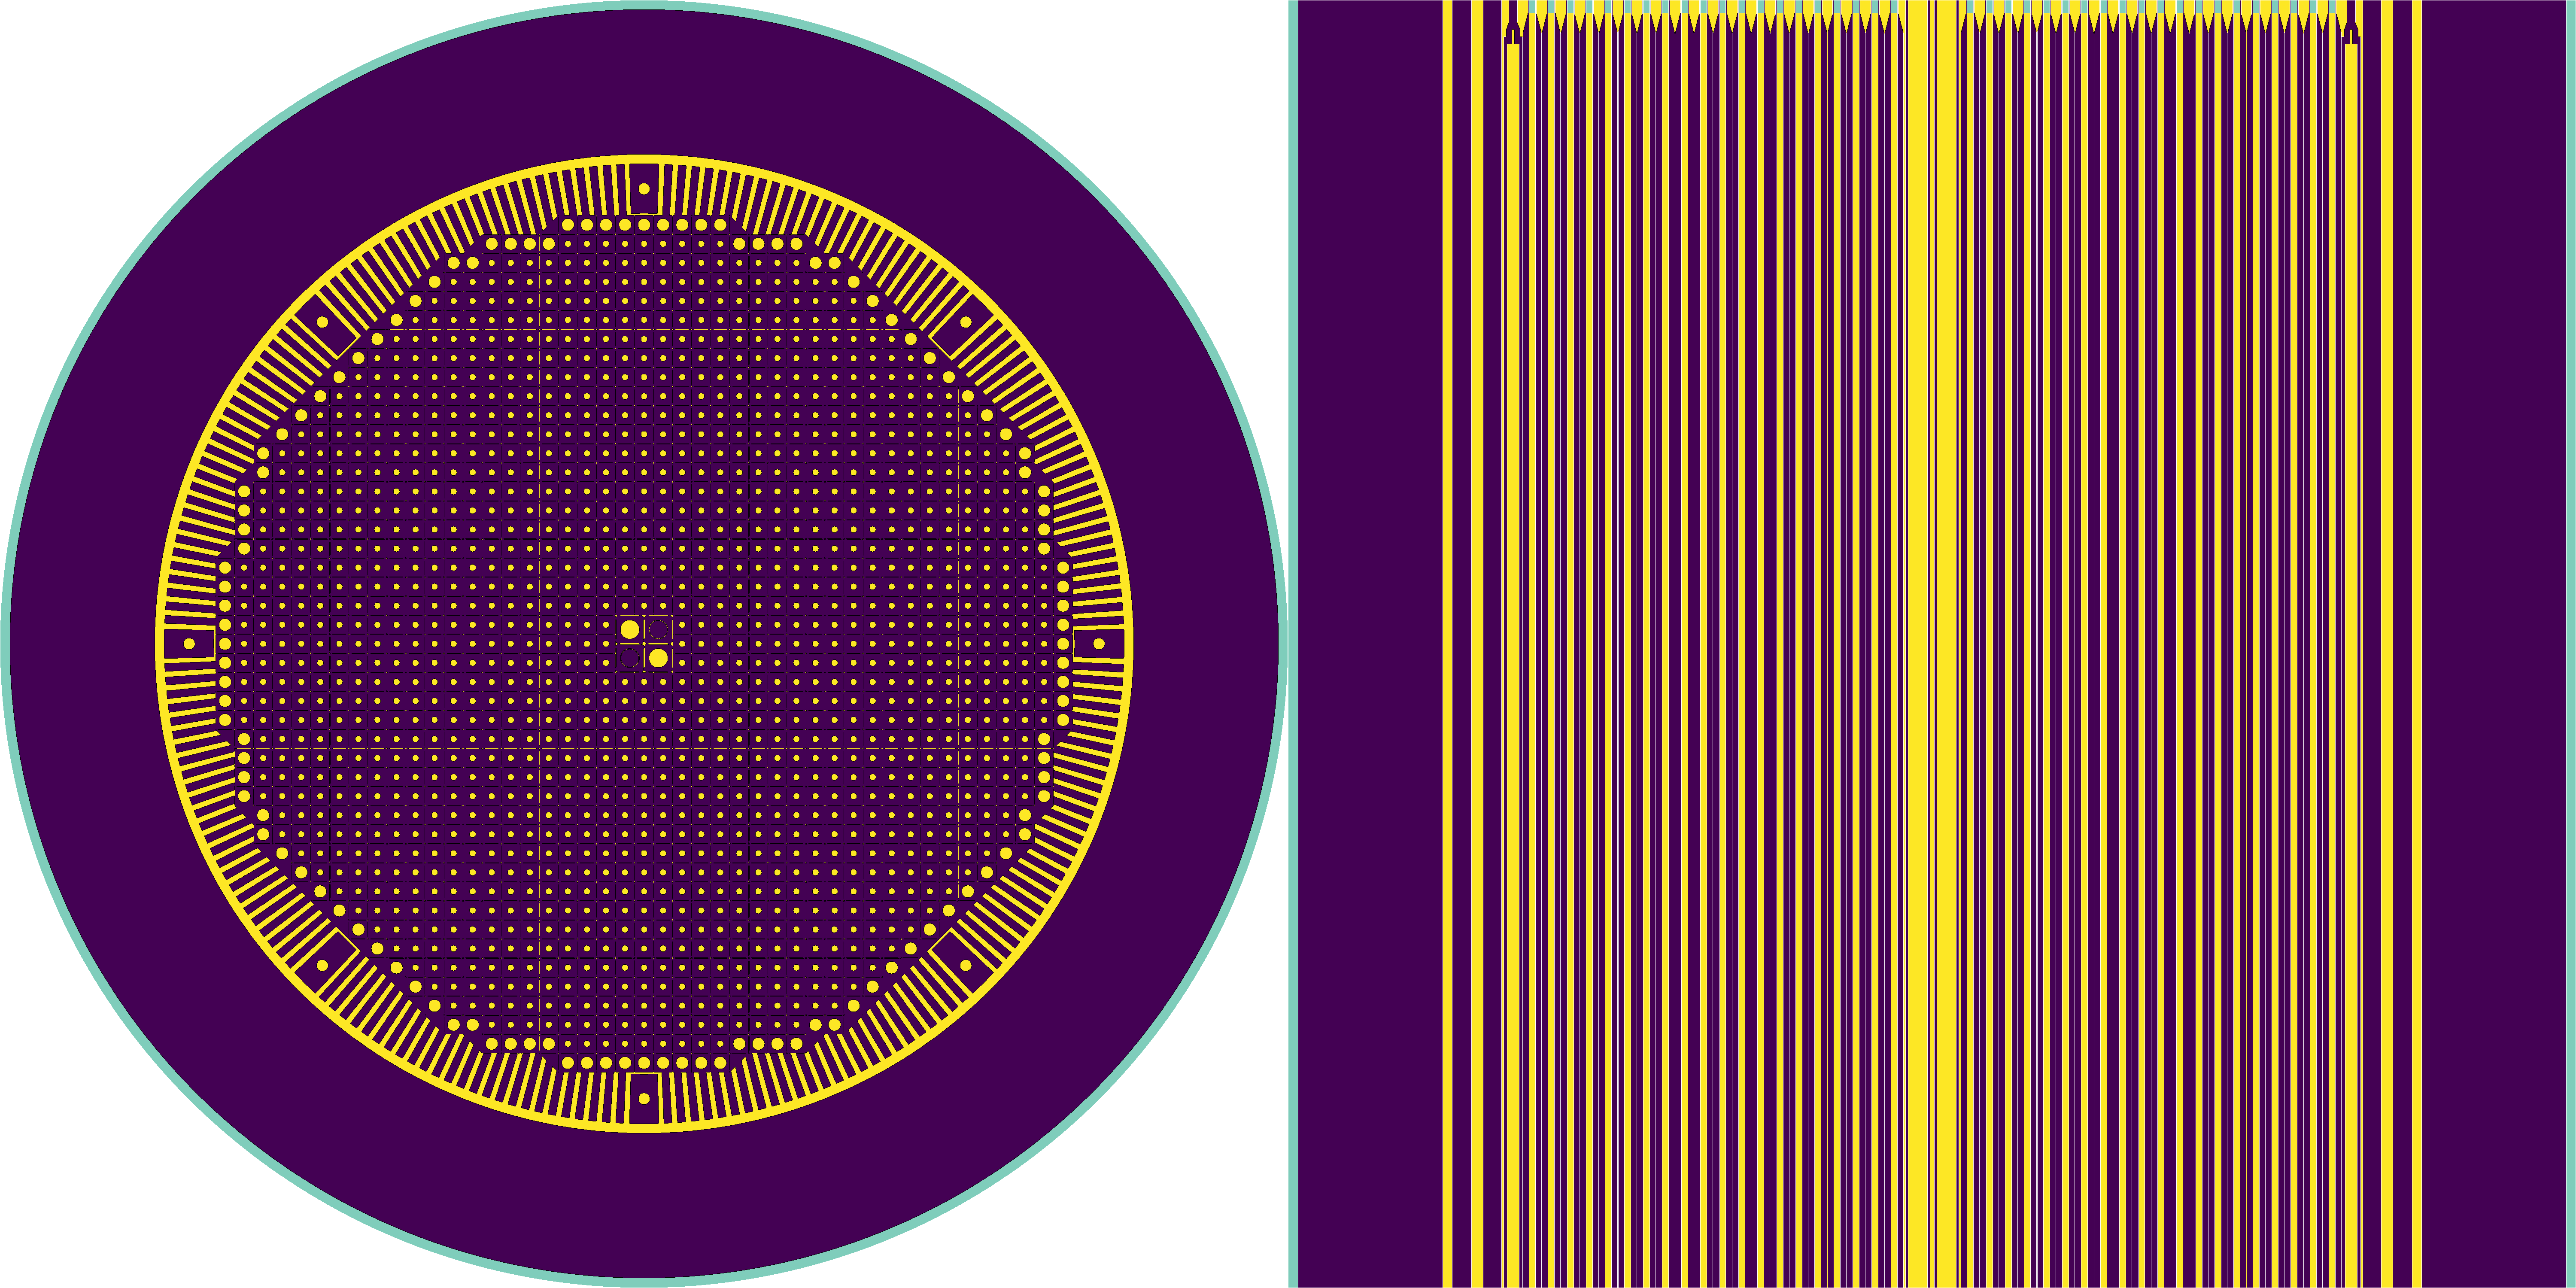
\includegraphics[width=\textwidth]{./images/geometry_main_views.png}
	\caption{An $XY$ (left) and $XZ$ (right) sections of \gls{MSBR} model. 
		The violet color represents graphite, the yellow - fuel salt 	
		\cite{rykhlevskii_full-core_2017}.}
\end{figure}
\end{textblock*}
\end{frame}

\begin{frame}
\frametitle{Moderator element geometry (Zone I)}
\begin{textblock*}{12.5cm}(0.1cm,1.9cm) % {block width} (coords)
\begin{figure}[t]
\includegraphics[width=\textwidth]{./images/zone_I_mesh.png}
\vspace{-5mm}
\caption{Molten Salt Breeder Reactor Zone I unit cell geometry from the 
	reference \cite{robertson_conceptual_1971} (left) and Serpent model 
	(right) \cite{rykhlevskii_full-core_2017}.}
\end{figure}
\end{textblock*}

\end{frame}

\begin{frame}
\frametitle{Graphite channels geometry}
\begin{textblock*}{12.5cm}(0.02cm,2.0cm) % {block width} (coords)
\begin{figure}[t]
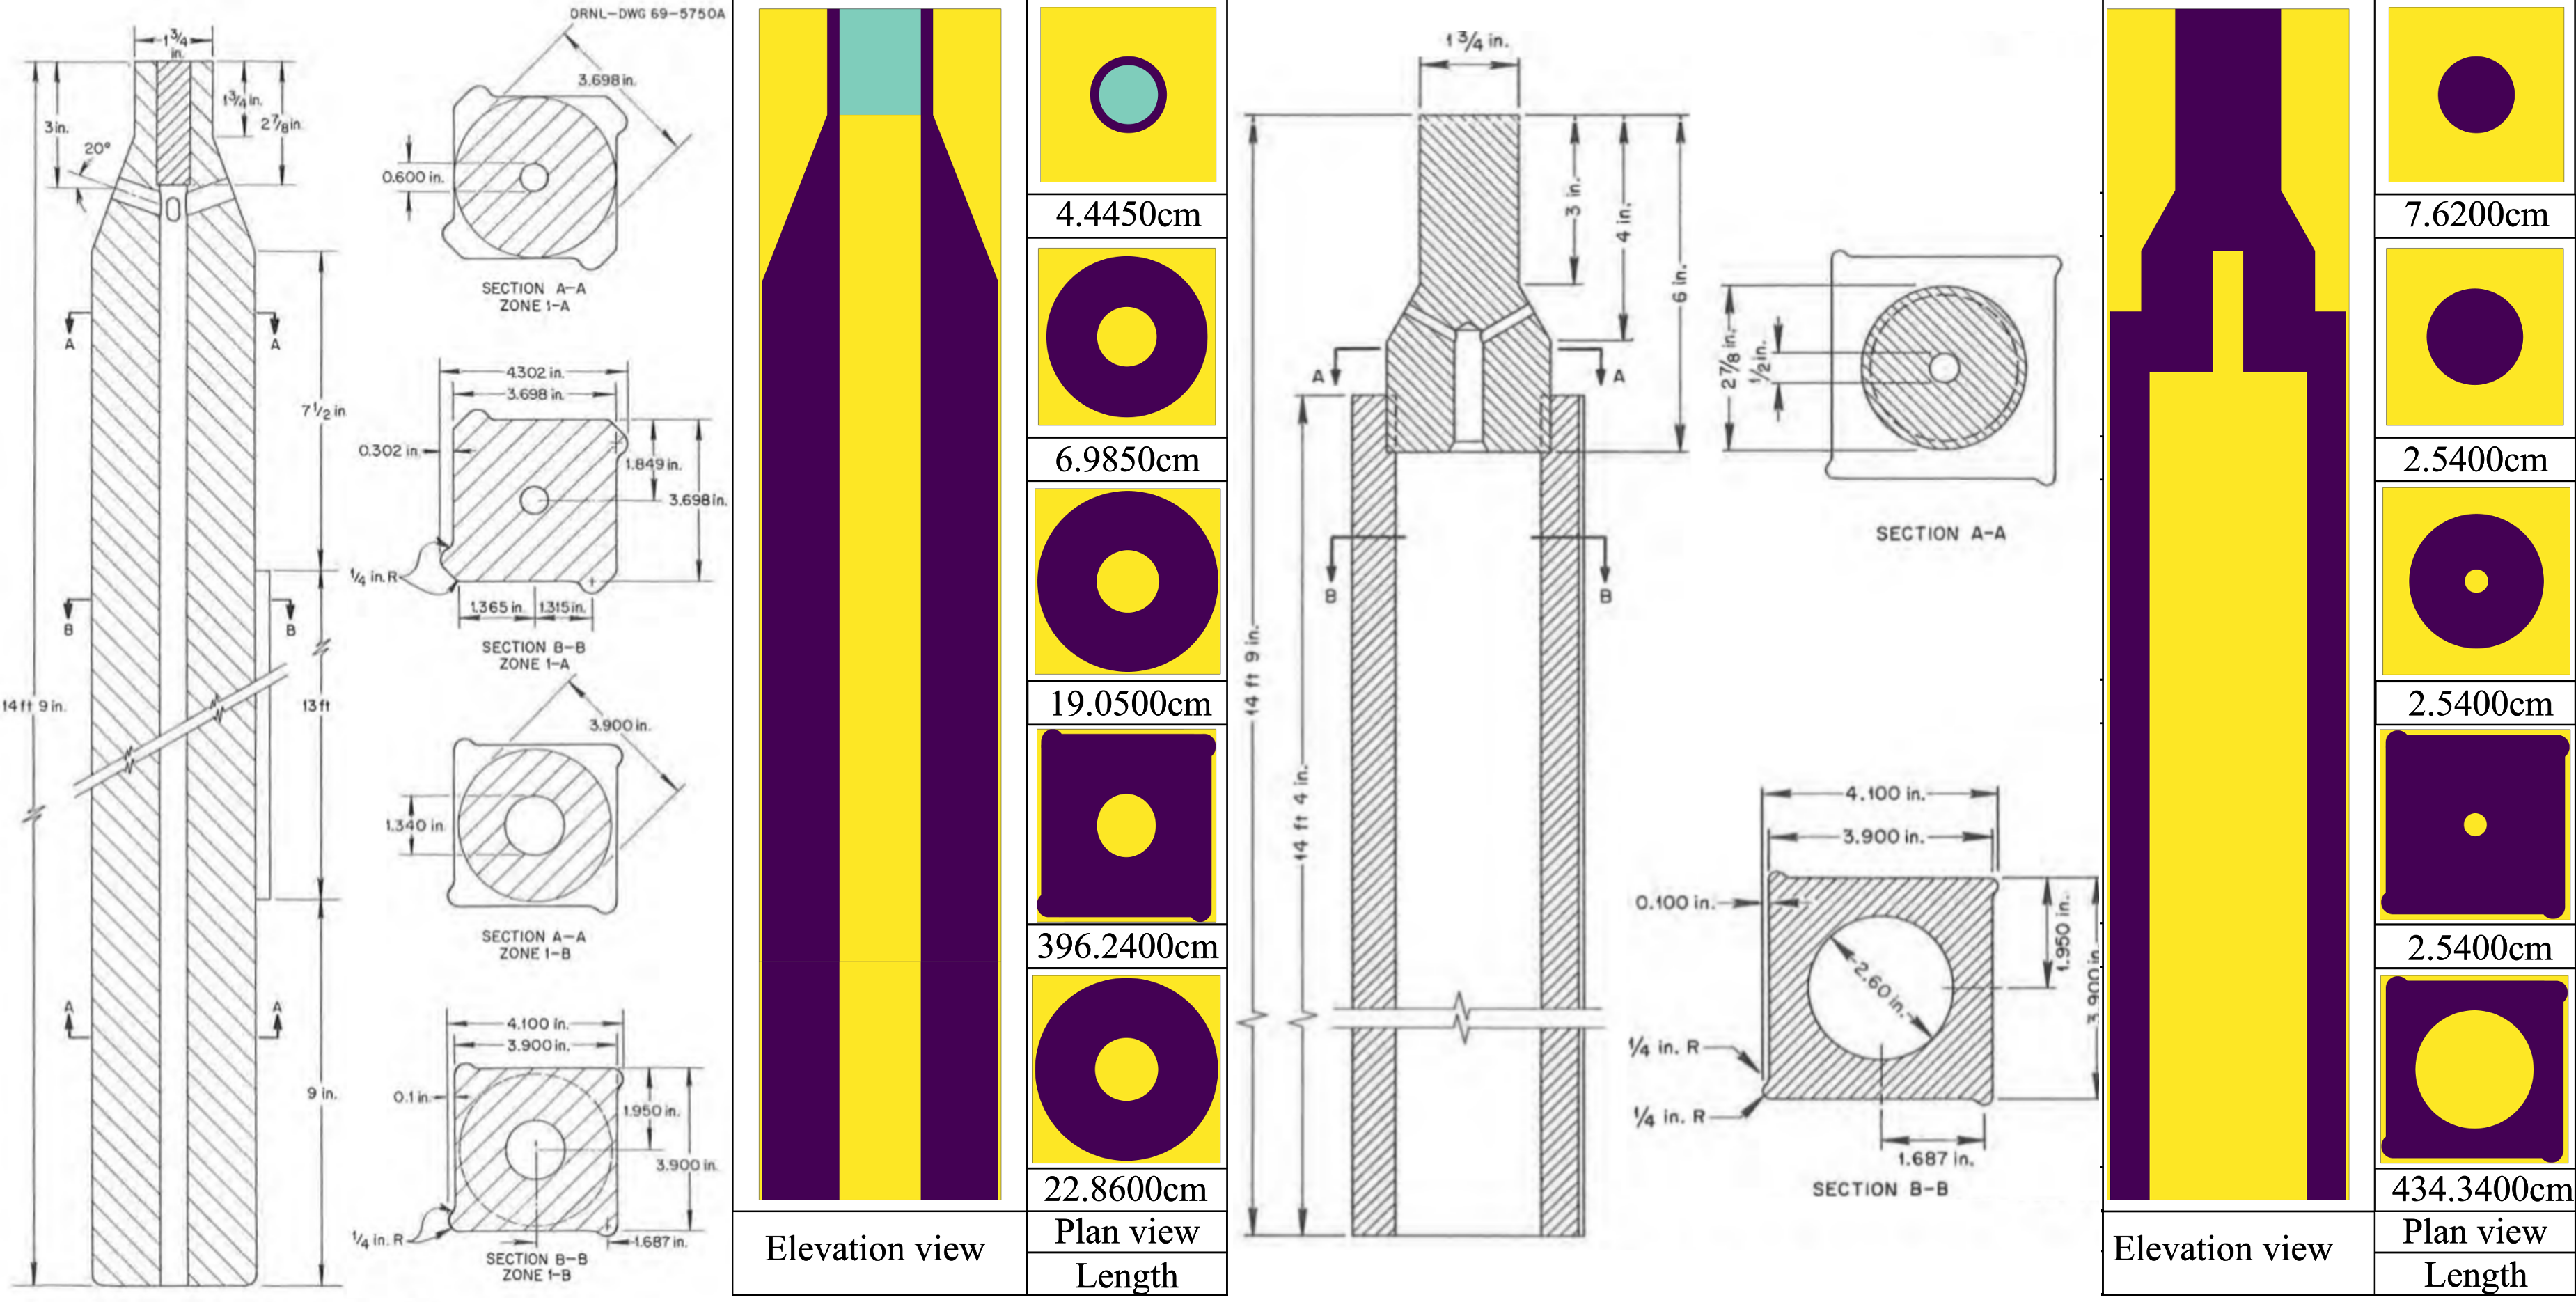
\includegraphics[width=1.02\textwidth]{./images/detailed_element_xz.png}
\vspace{-5mm}
\caption{Zone I (left) and Zone II (right) reference design 
\cite{robertson_conceptual_1971} and Serpent 
model \cite{rykhlevskii_full-core_2017}.}
\end{figure}
\end{textblock*}

\end{frame}


\begin{frame}
\frametitle{$k_{eff}$ dynamics during 60 years of MSBR operation}
\vspace{-3mm}
\begin{columns}
	\column{4.3cm}
	\begin{block}{Analysis assumptions}
		\fontsize{7}{9}\selectfont
		\begin{itemize}
			\item Full-core Serpent model
			\item Fine time resolution (\textbf{3-day} depletion steps)
			\item Slowly extracted elements are removed at the end of the 
			cycle time (e.g., 50 days for RE)
			\item FP removal efficiency \textbf{fixed, ideal}
			\item All $^{233}$Pa removed and \textbf{equal mass of $^{233}$U} 
			fed to the core
			\item Fresh fertile material feed ($^{232}$Th) to maintain salt 
			inventory
		\end{itemize}
	\end{block}
	\vspace{-2mm}
	\begin{block}{Main findings}
	\fontsize{7}{9}\selectfont
	\begin{itemize}
		\item Strong absorbers ($^{234}$U) and fissile materials ($^{235}$U) 
		are built-up
		\item $k_{eff}$ stabilizes after $\approx6$ years
	\end{itemize}  
	\end{block}  	
	
	\column{8cm}
	\begin{figure}[ht!] 
	\begin{overprint}
	\onslide<1>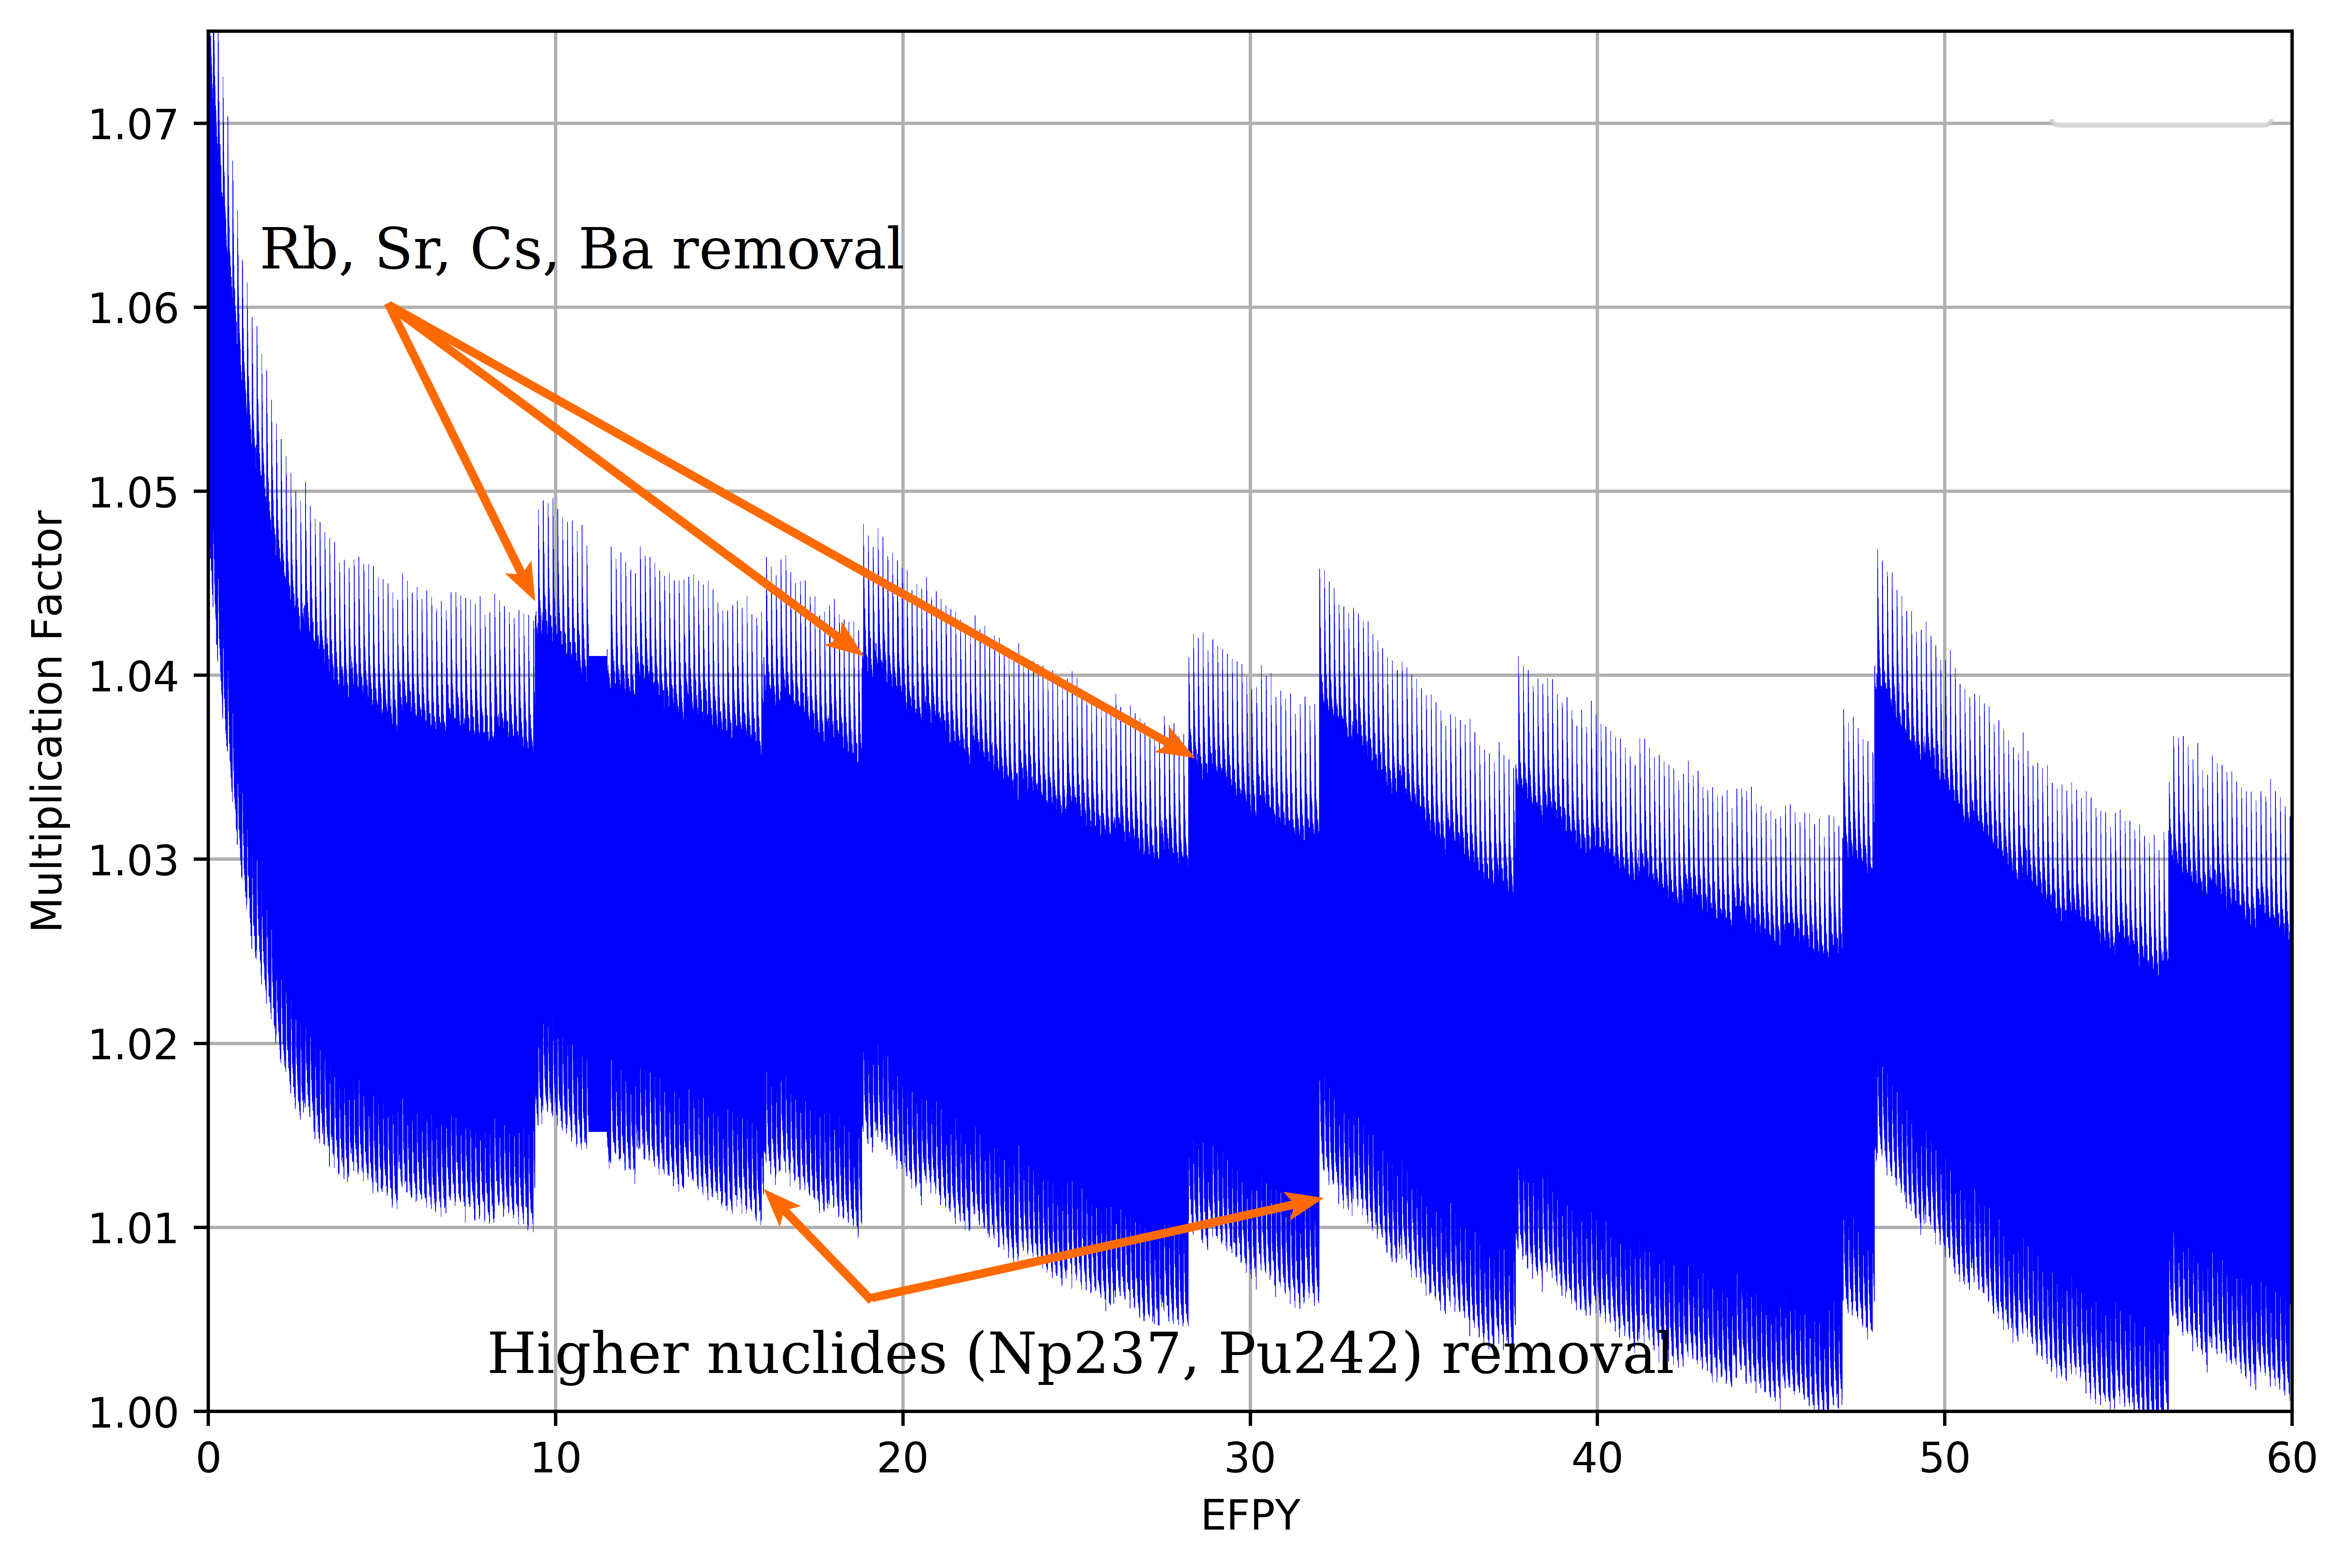
\includegraphics[width=\textwidth]{../dissertation/figures/ch3/keff.png}
	\vspace{-2mm}
	\caption{Effective multiplication factor dynamics for the full-core 
	\gls{MSBR} model \cite{rykhlevskii_modeling_2019}.}
	\onslide<2>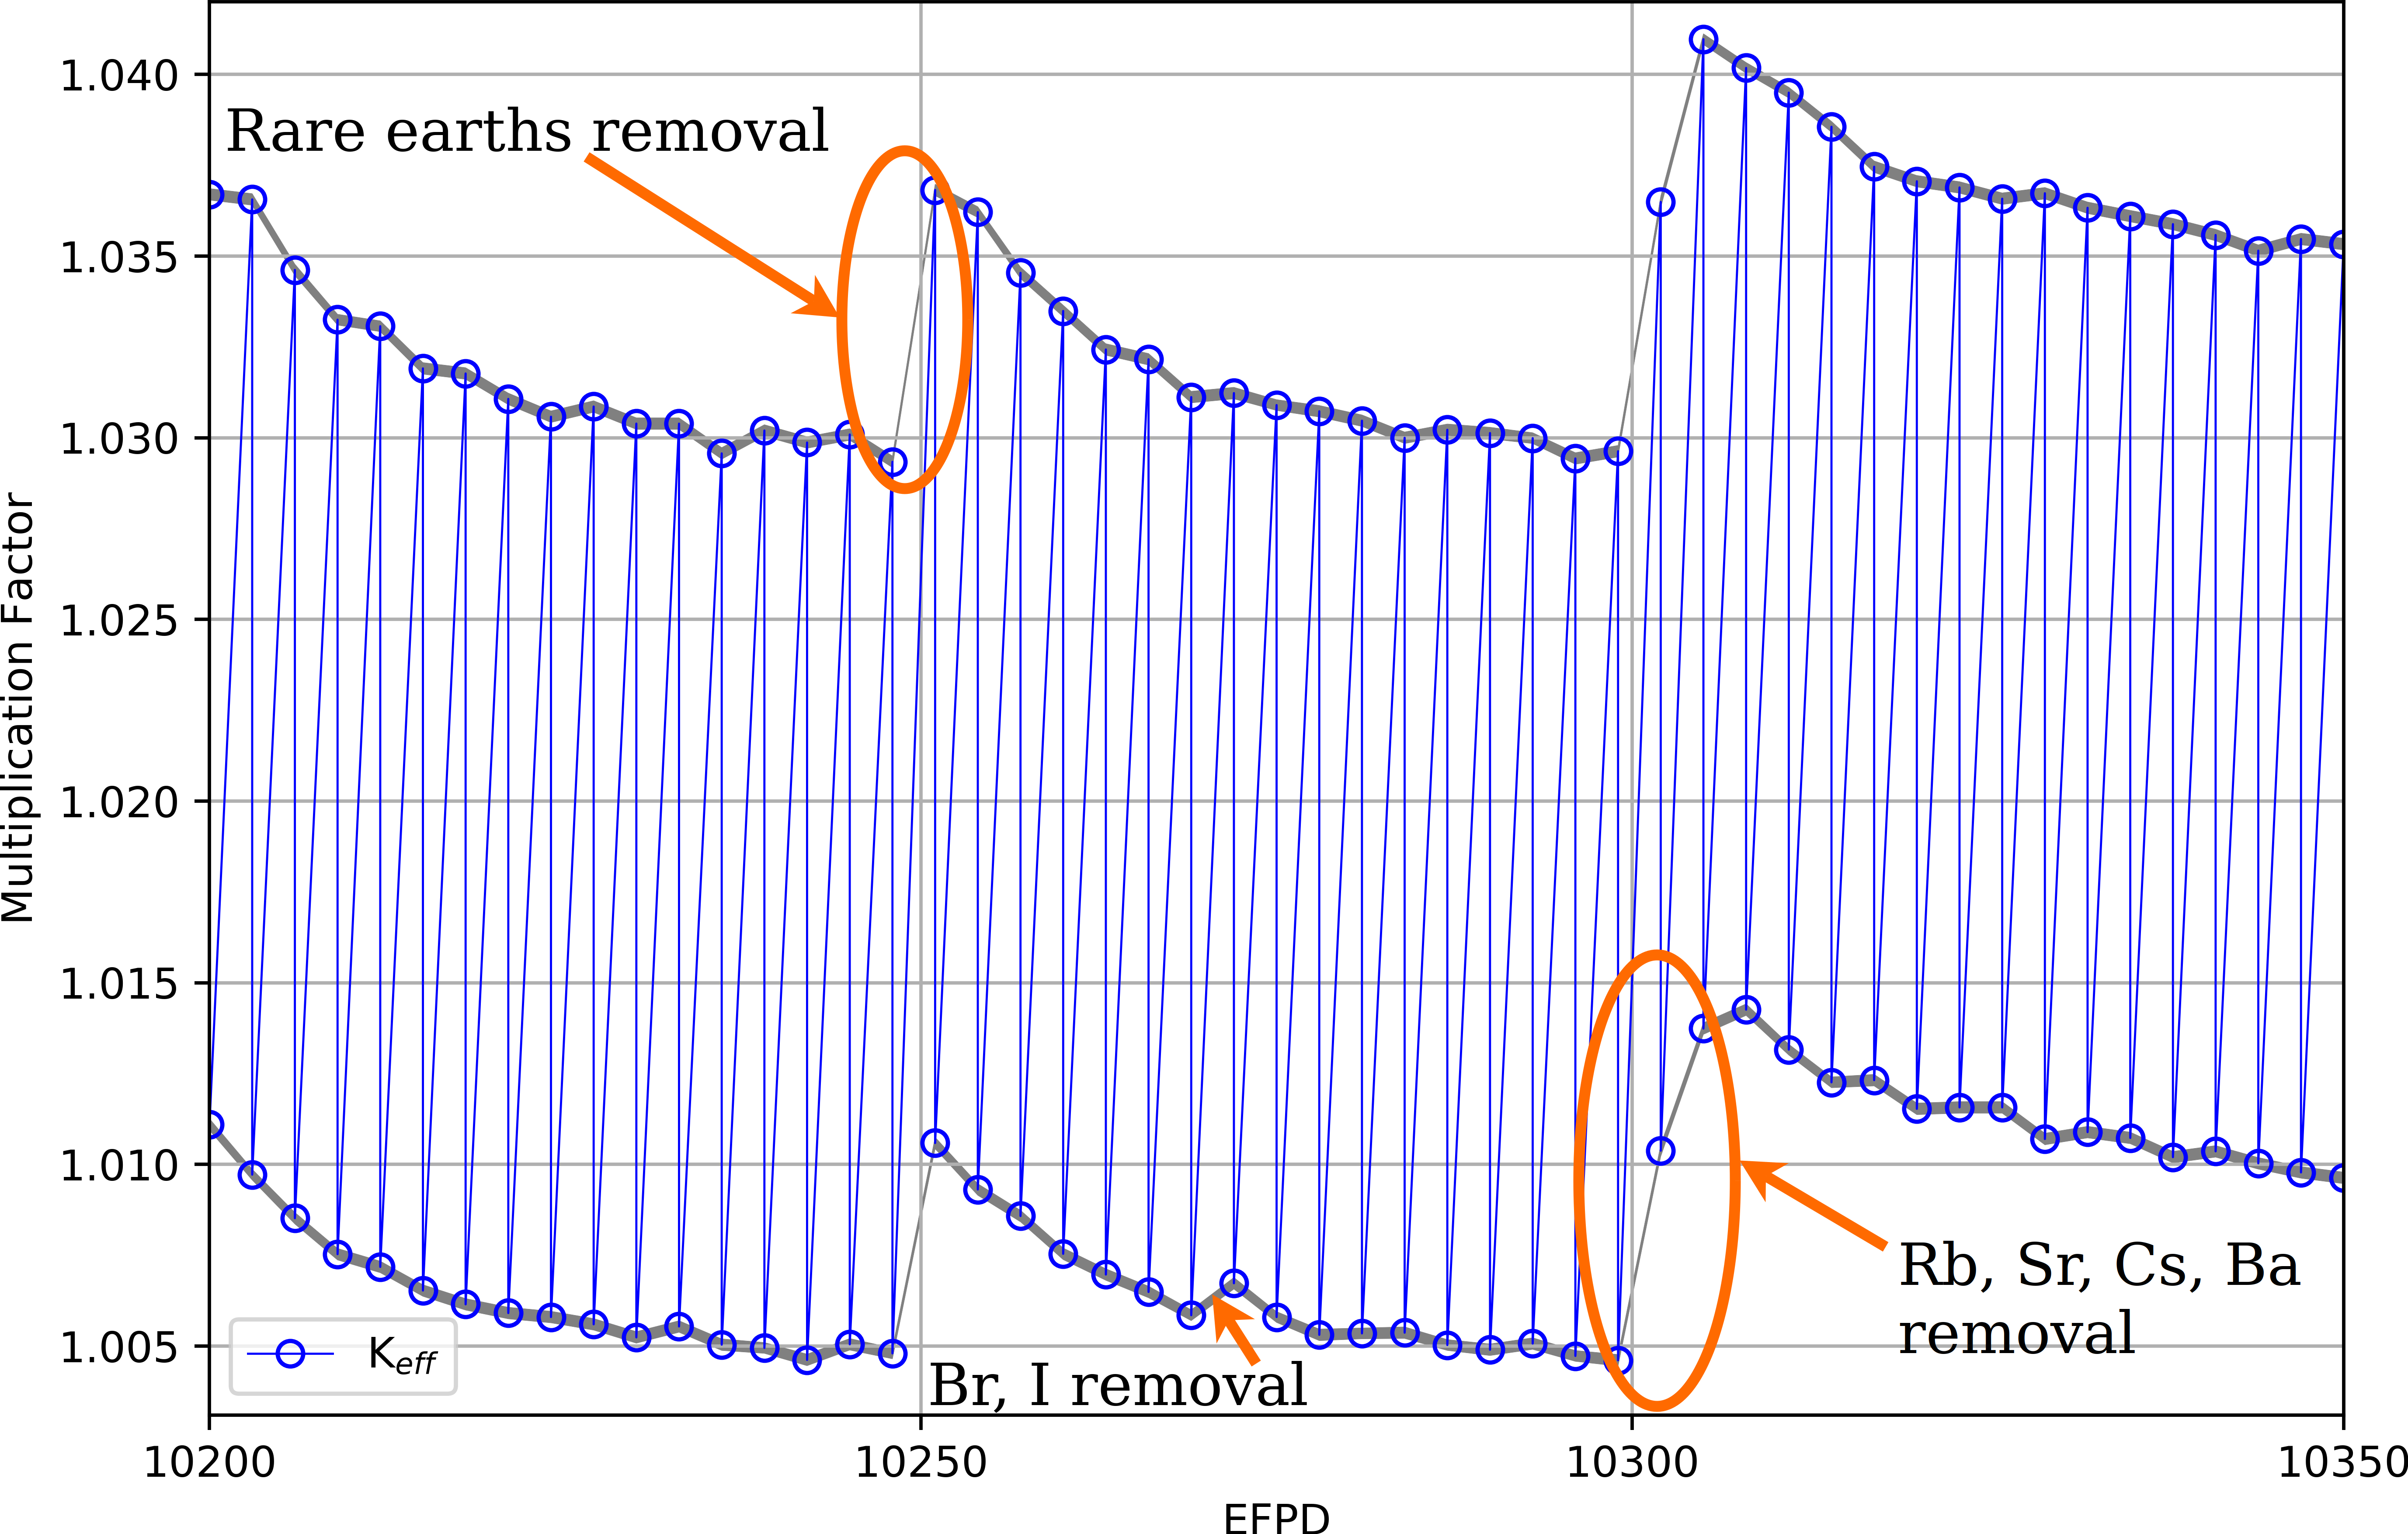
\includegraphics[width=\textwidth]{../dissertation/figures/ch3/keff_zoomed.png}
	\vspace{-0.5mm}
	\caption{\textbf{Zoomed} effective multiplication factor dynamics for the 
	full-core \gls{MSBR} model \cite{rykhlevskii_modeling_2019}.}
	\end{overprint}
	\end{figure}
	
\end{columns}
\end{frame}

\begin{frame}
\frametitle{Fuel salt composition evolution in the MSBR}
\begin{textblock*}{12.8cm}(0.07cm,2.6cm) % {block width} (coords)
\begin{columns}
	\column[t]{7cm}
	\vspace{-0.35in}
	\begin{figure}[t]
		\hspace{-5mm}
		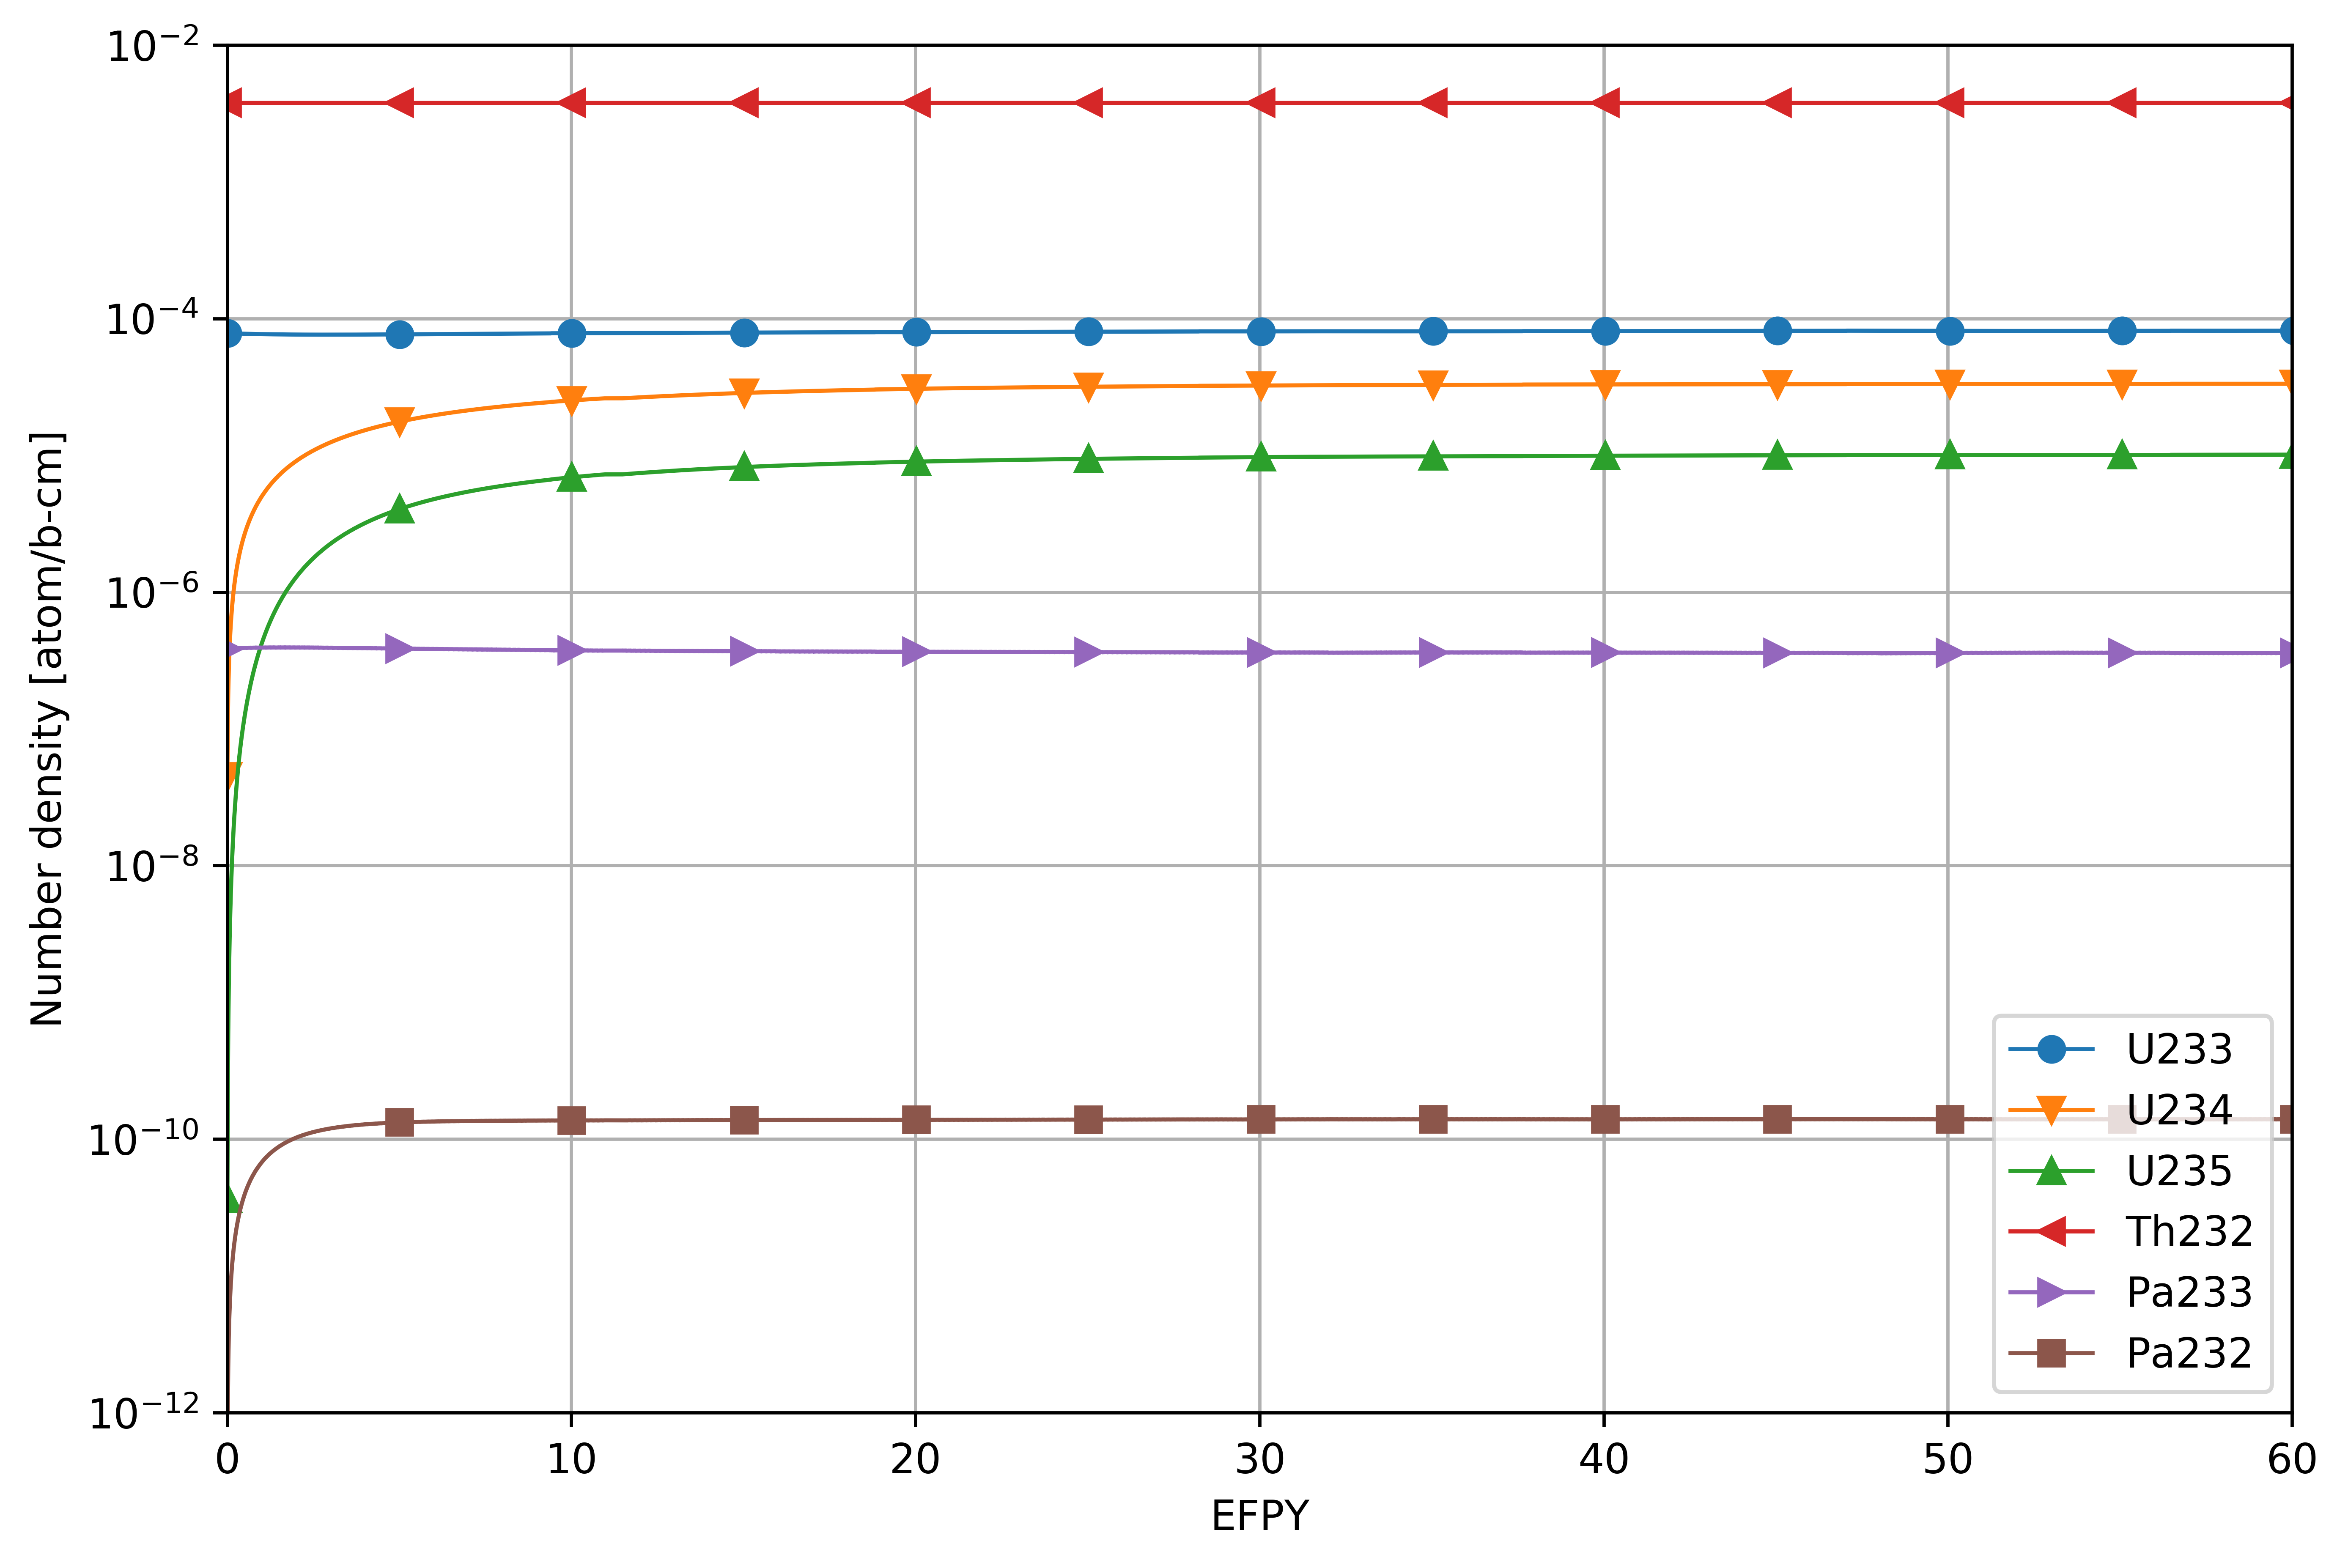
\includegraphics[height=0.7\textheight]{../dissertation/figures/ch3/major_isotopes_adens.png}
		\vspace{-0.15in}
		\caption{Normalized number density of major isotopes in the salt
			during 60 years of operation \cite{rykhlevskii_advanced_2018}.}
	\end{figure}
	
	\column[t]{4.5cm}
	\fontsize{7}{9}\selectfont
		\vspace{-3mm}
	\begin{itemize}
		\item<1-> Neutron poisons ($^{234}$U, $^{232}$Pa) accumulation has 
		negative impact on neutronics
		\item<1-> New fissile materials ($^{235}$U, $^{239}$Pu) improved core 
		performance
		\item<1-> $^{233}$U number density almost constant ($\Delta m<0.8\%$) 
		after 16 years of operation
		\item<1-> $^{242}$Th feed rate \textbf{2.4 kg/d is consistent with 
		ORNL results (2.45 kg/d) \cite{betzler_personal_2017}}
		\item<2-> Neutron spectrum \textbf{hardens toward EOL} causing:
		\setbeamerfont*{itemize/enumerate body}{size=\footnotesize}
		\setbeamerfont*{itemize/enumerate subbody}{parent=itemize/enumerate 
		body}
		\setbeamerfont*{itemize/enumerate subsubbody}{parent=itemize/enumerate 
		body}
		\begin{itemize}
			\item<3-> Reduced $^{233}$U breeding
			\item<4->Temperature coefficient ($\alpha_T$) weakened 
			from $-1.64$ to $-1.58pcm/K$
			\item<5->16\% decline in total control rod worth (CRW)
		\end{itemize} 
	\end{itemize}
\end{columns}
\end{textblock*}
\end{frame}


\begin{frame}
\frametitle{Effect of fission products removal}       

\begin{figure}[t] % replace 't' with 'b' to force it to 
	\centering
	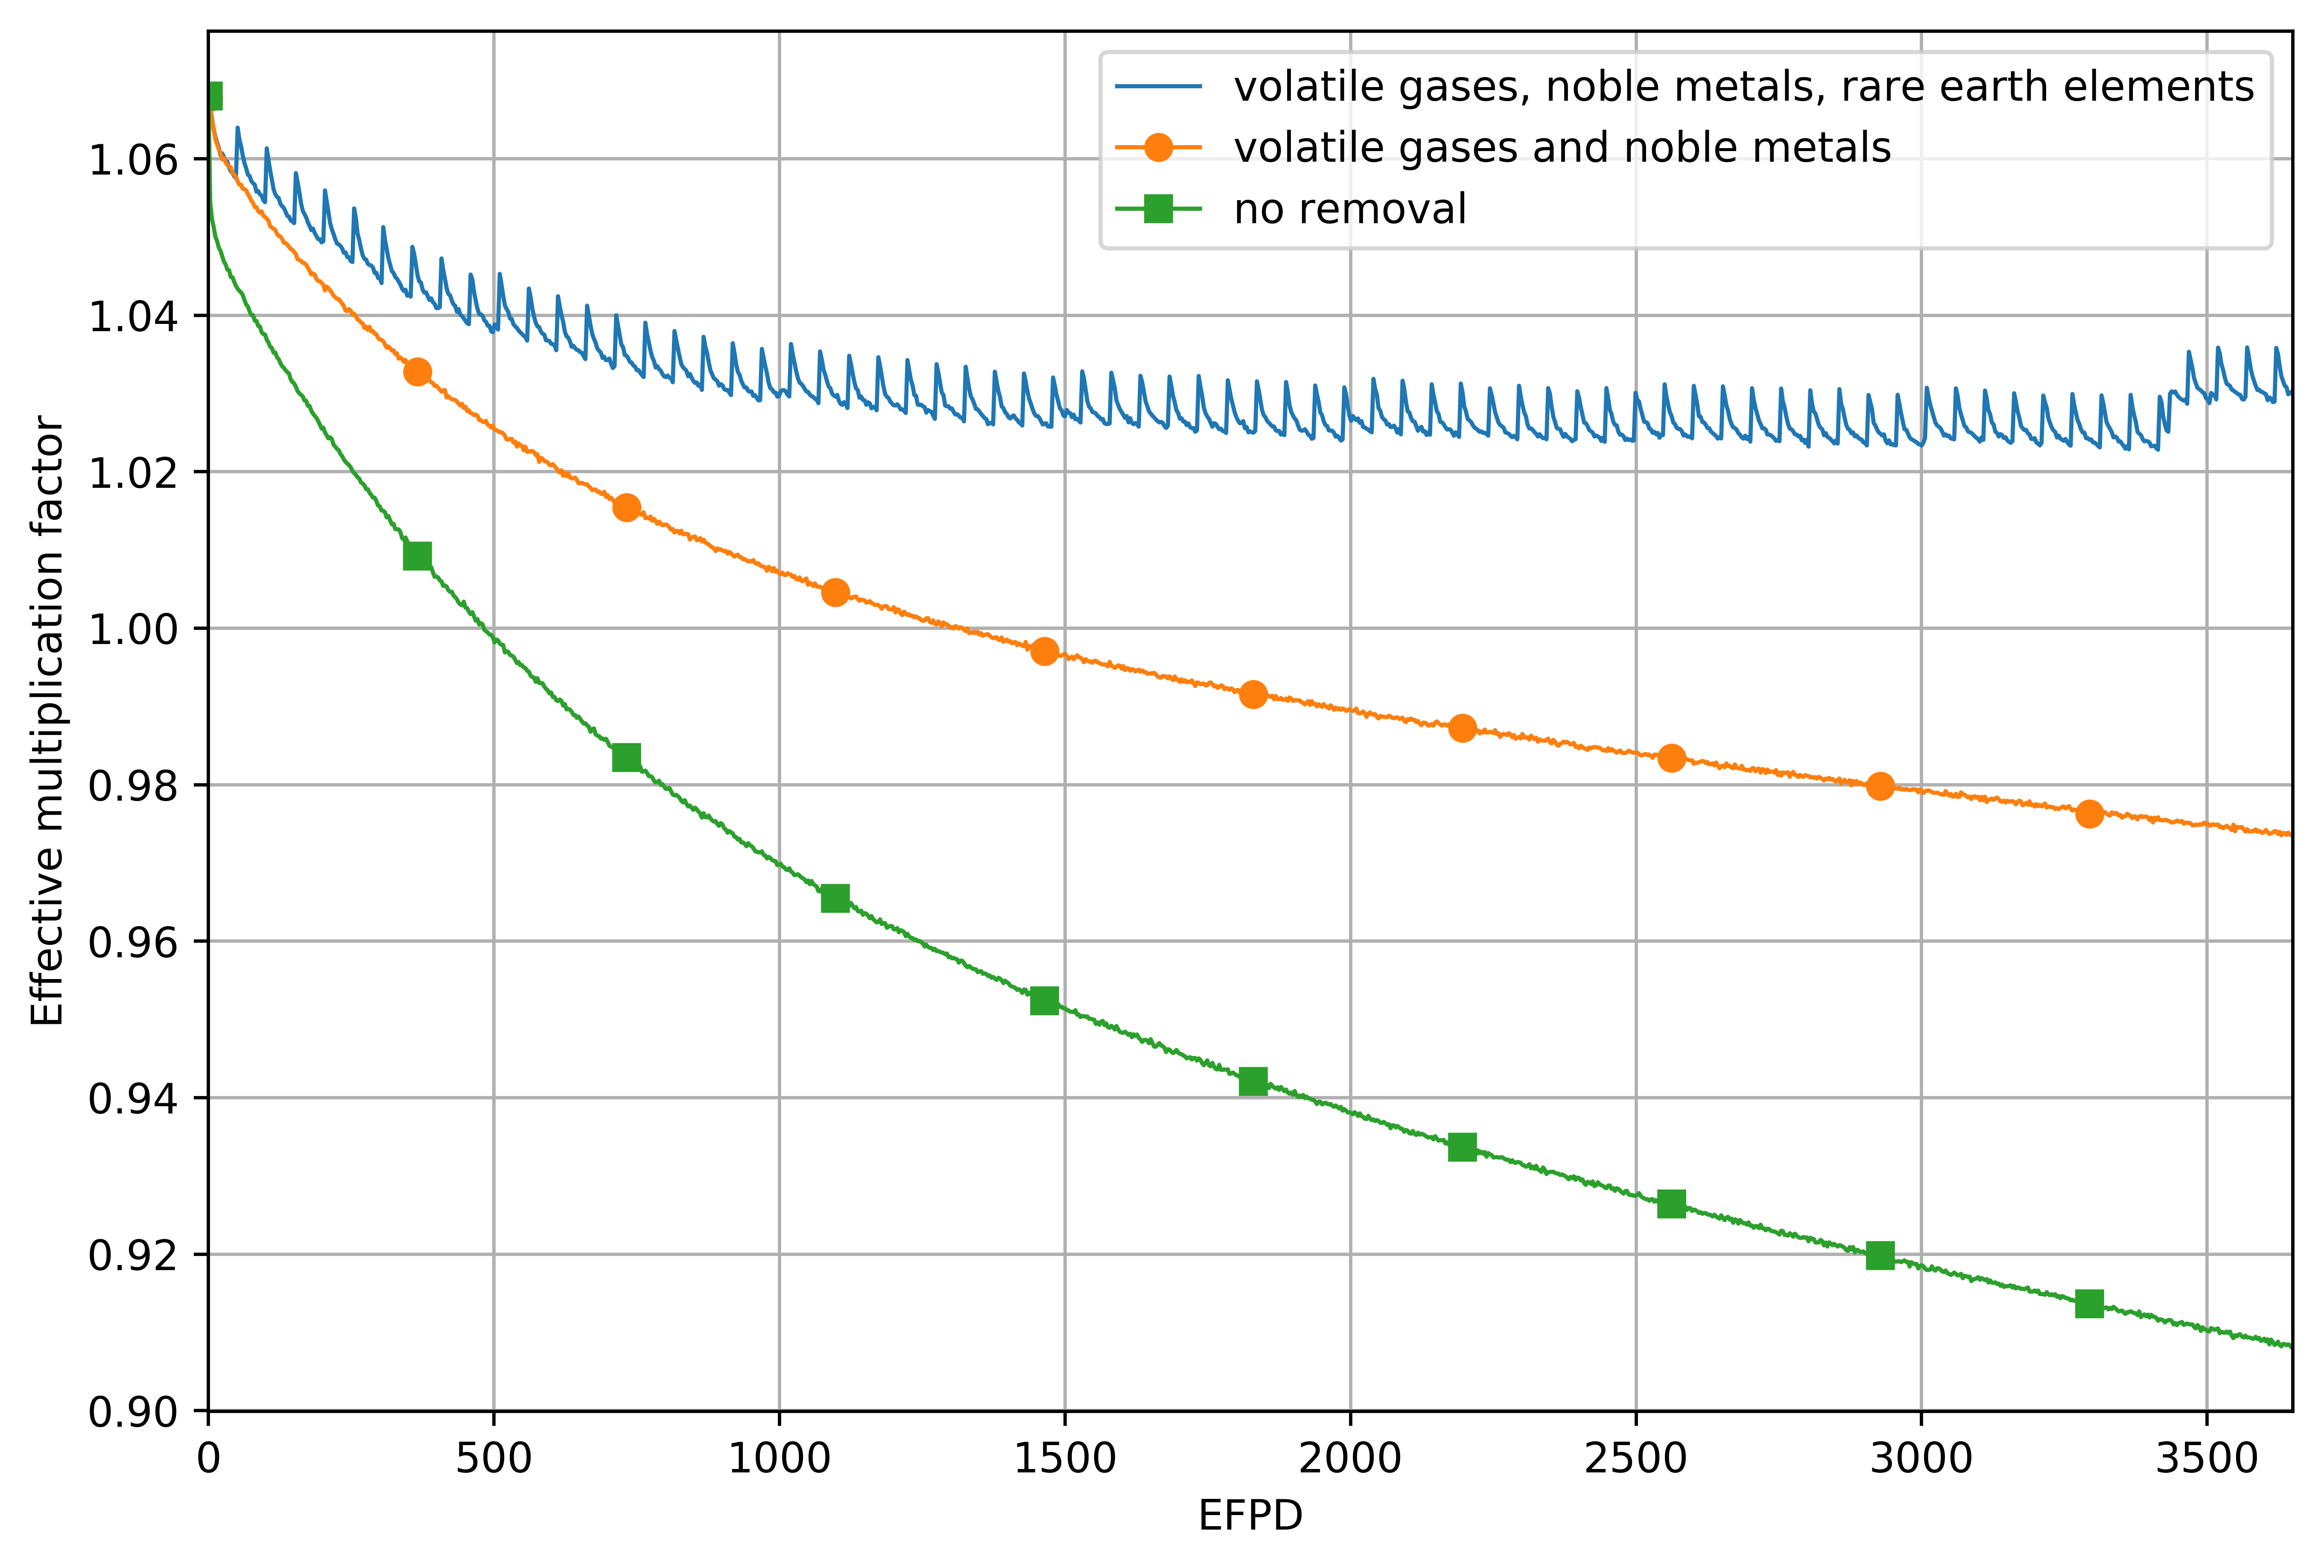
\includegraphics[width=0.9\textwidth]{../dissertation/figures/ch3/keff_rem_cases.png}
	 
		\vspace{-3mm}
	\caption{SaltProc-calculated effective multiplication factor for the 
	full-core \gls{MSBR} model with removal of various fission product groups 
	over 10	years of operation \cite{rykhlevskii_modeling_2019}.}
\end{figure}

\end{frame}



\subsection{Lifetime-long depletion: \gls{TAP} MSR}

\begin{frame}
\frametitle{TAP concept design}

\begin{textblock*}{12.7cm}(0.25cm,1.8cm) % {block width} (coords)
	
	\begin{columns}
		\column[t]{5cm}
		\vspace{+5mm}
		%%%%%%%%%%%%%%%%%%%%%%%%%%%%%%%%%%%%%%%%
		\begin{table}[h!]
			\fontsize{7}{9}\selectfont
			\caption{Summary of principal data
				\cite{transatomic_power_corporation_technical_2016}. }
			\vspace{-2mm}
			\begin{tabularx}{\textwidth}{ X  X }
				\hline
				Thermal power				           		& 1250 MW$_{th}  
				$       
				\\ 
				Electric power		                		& 520 MW$_e  
				$ 			 
				\\ 
				Gross thermal efficiency        			& 
				44\%     				 
				\\  
				Outlet temperature							& 
				620$^{\circ}$C         
				\\ 
				Fuel salt components                   & 
				LiF-UF$_4$				 \\  
				Fuel salt composition                  & 72.5-27.5 
				mole\%			 
				\\  
				Startup fissile material                     & 5\% 
				$^{235}$U          	 \\
				Moderator                              & ZrH$_{1.66}$ rods  \\
				Neutron spectrum						& 
				\textbf{thermal/epithermal}                 \\
				Moderator-to-fuel ratio						& 
				\textbf{varies in (0.1099, 1.0)}                 \\
				\hline
			\end{tabularx}
			\label{tab:tap_tab}
		\end{table}
		%%%%%%%%%%%%%%%%%%%%%%%%%%%%%%%%%%%%%%%%%%%%%%%%
		
		\column[t]{6.5cm}
		\hspace{-9mm}
		\begin{figure}      
			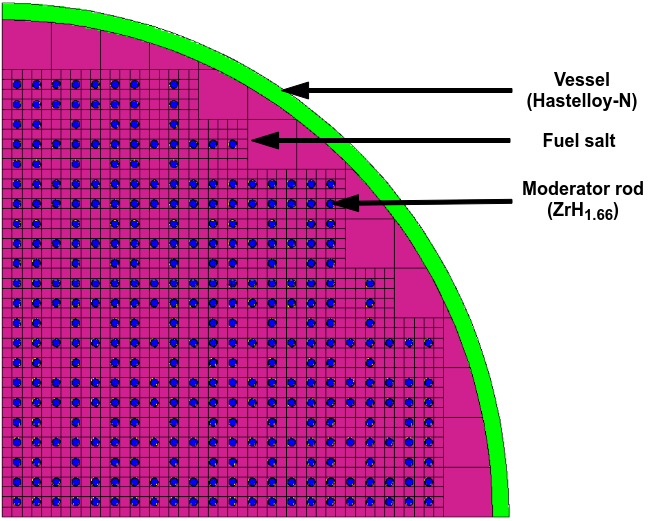
\includegraphics[height=0.79\textwidth]{../dissertation/figures/ch4/tap_core_ornl.png}
			\caption{The \gls{TAP} \gls{MSR} schematic core view showing 
				moderator rods configuration at \gls{BOL} 
				\cite{betzler_assessment_2017-1}.}
		\end{figure}
	\end{columns}
	
\end{textblock*}

\end{frame}

\begin{frame}
\frametitle{\gls{TAP} concept full-core high-fidelity Serpent model}
\begin{textblock*}{12.6cm}(0.1cm,1.8cm) % {block width} (coords)
\begin{figure}[htp!] % replace 't' with 'b' to 
	\begin{overprint}
		\onslide<1>\centerline{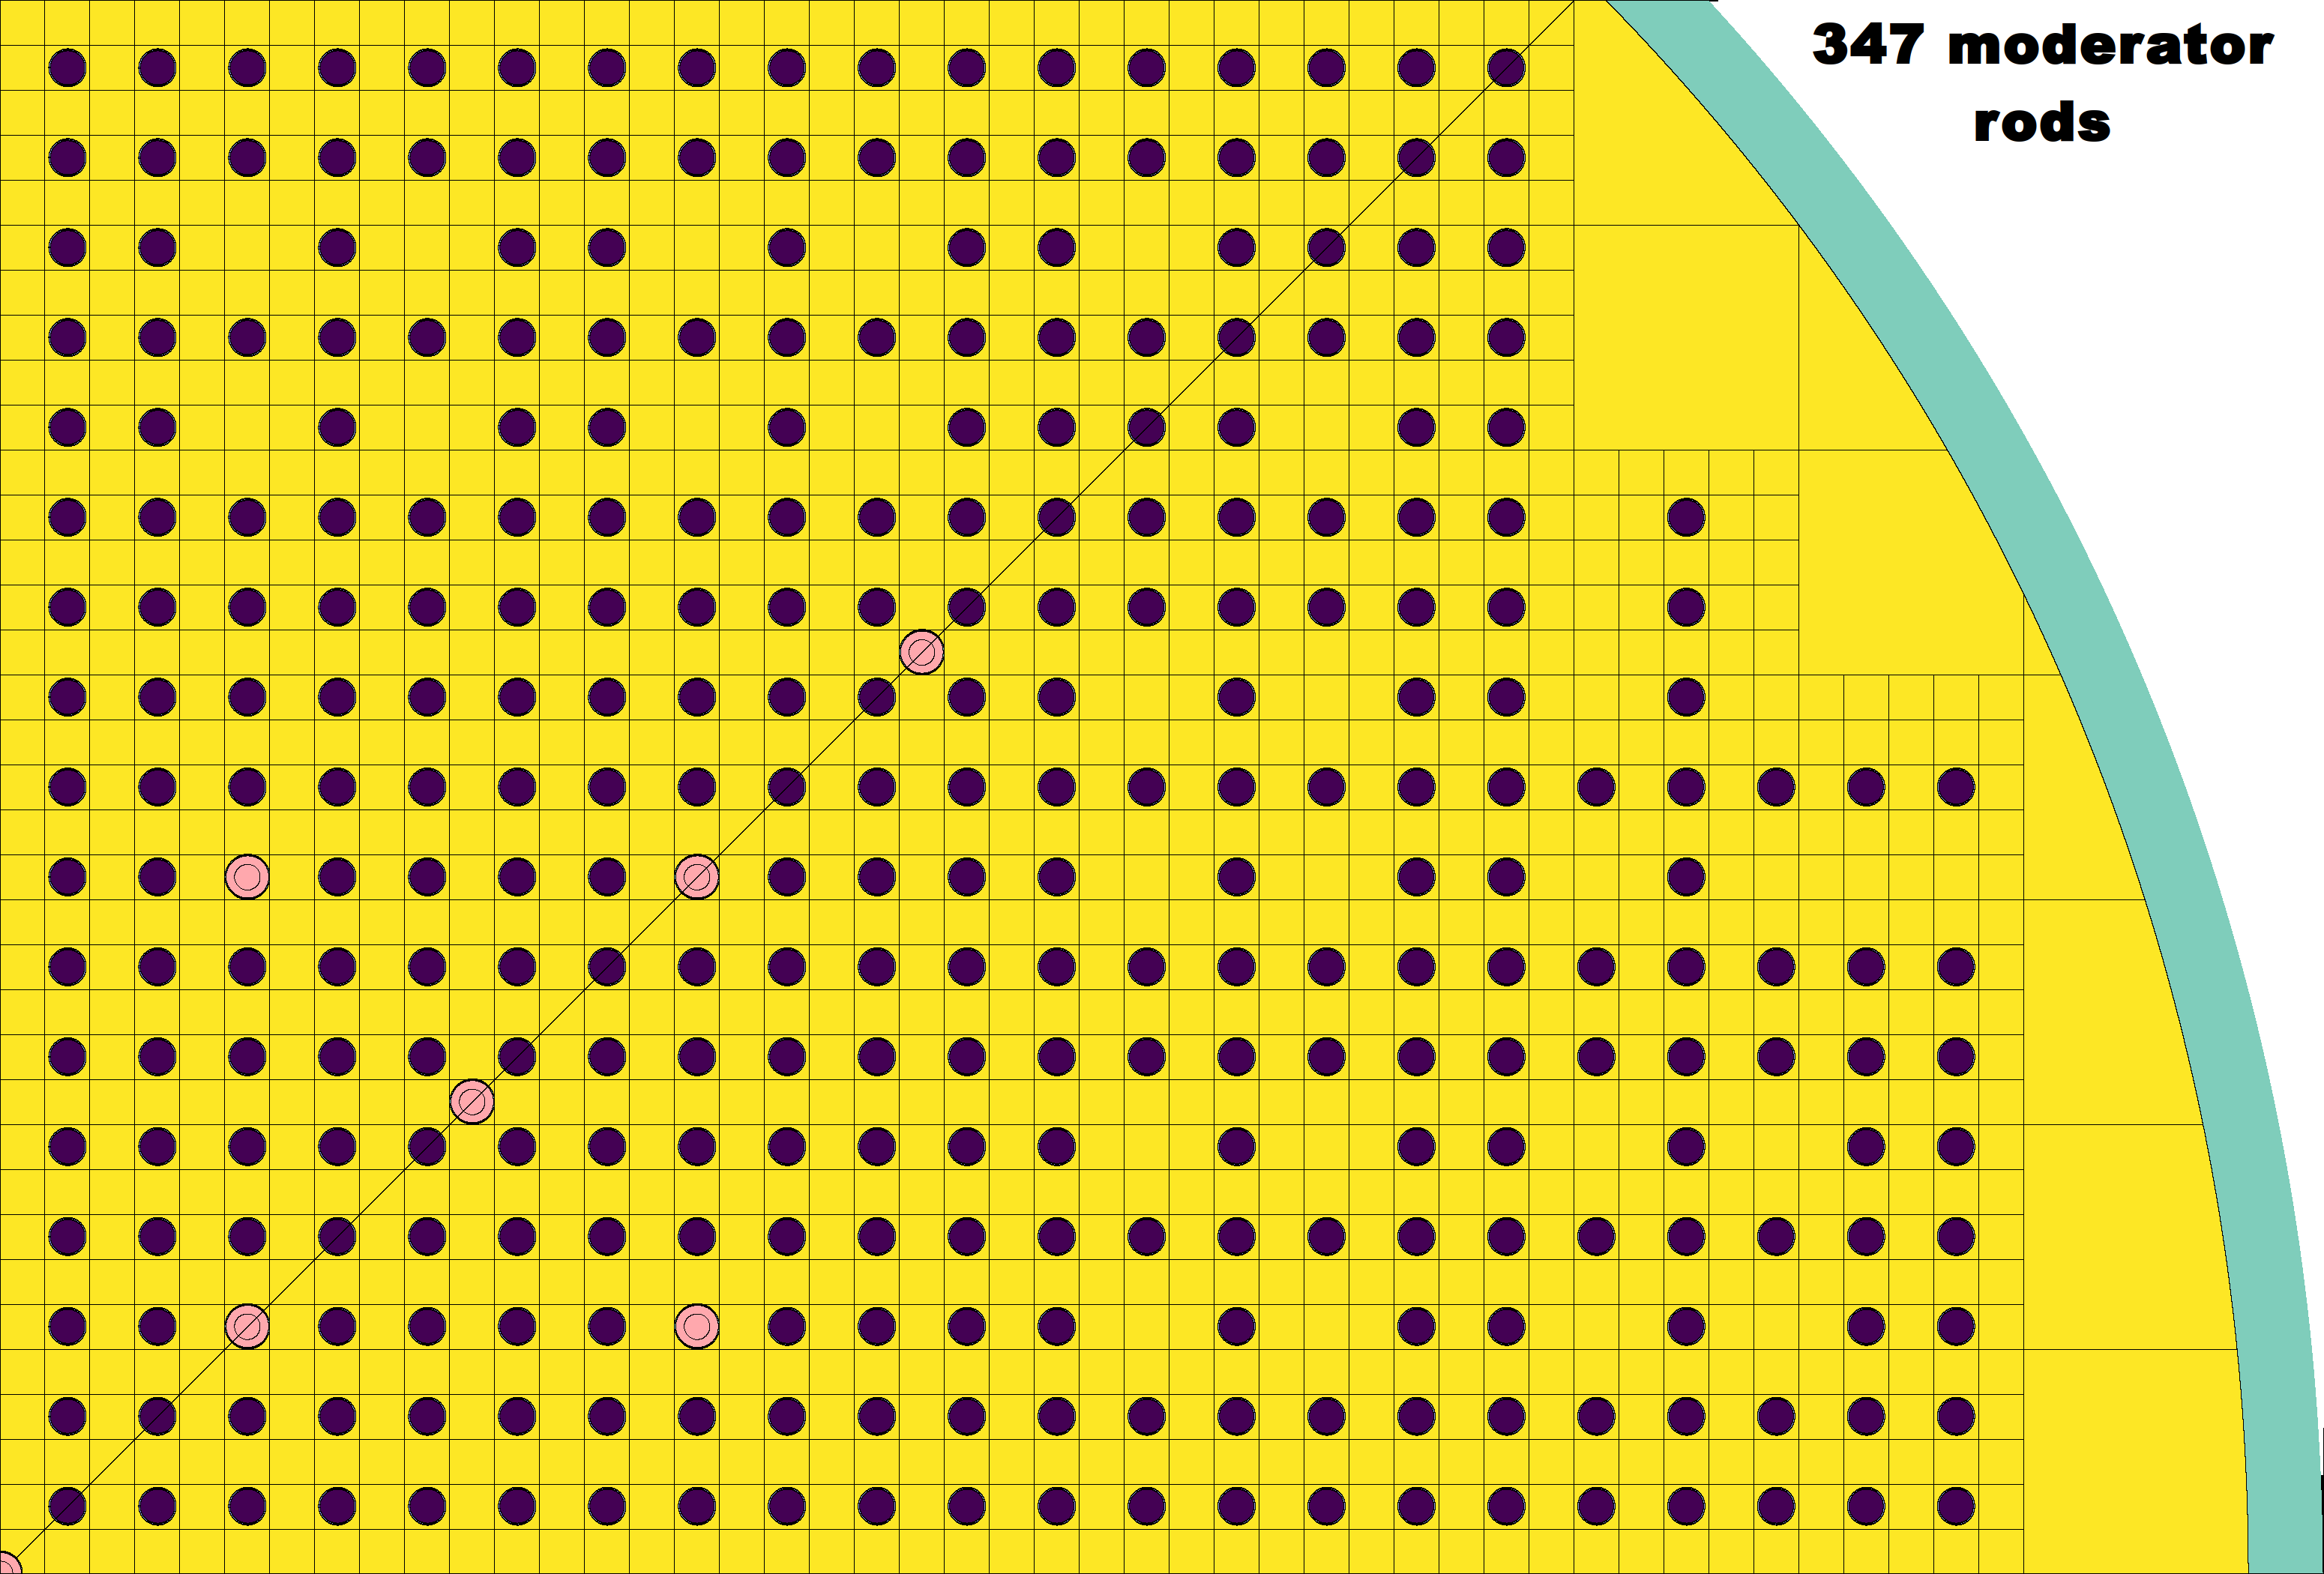
\includegraphics[height=0.75\textheight]{./images/347_base.png}}
		\onslide<2>\centerline{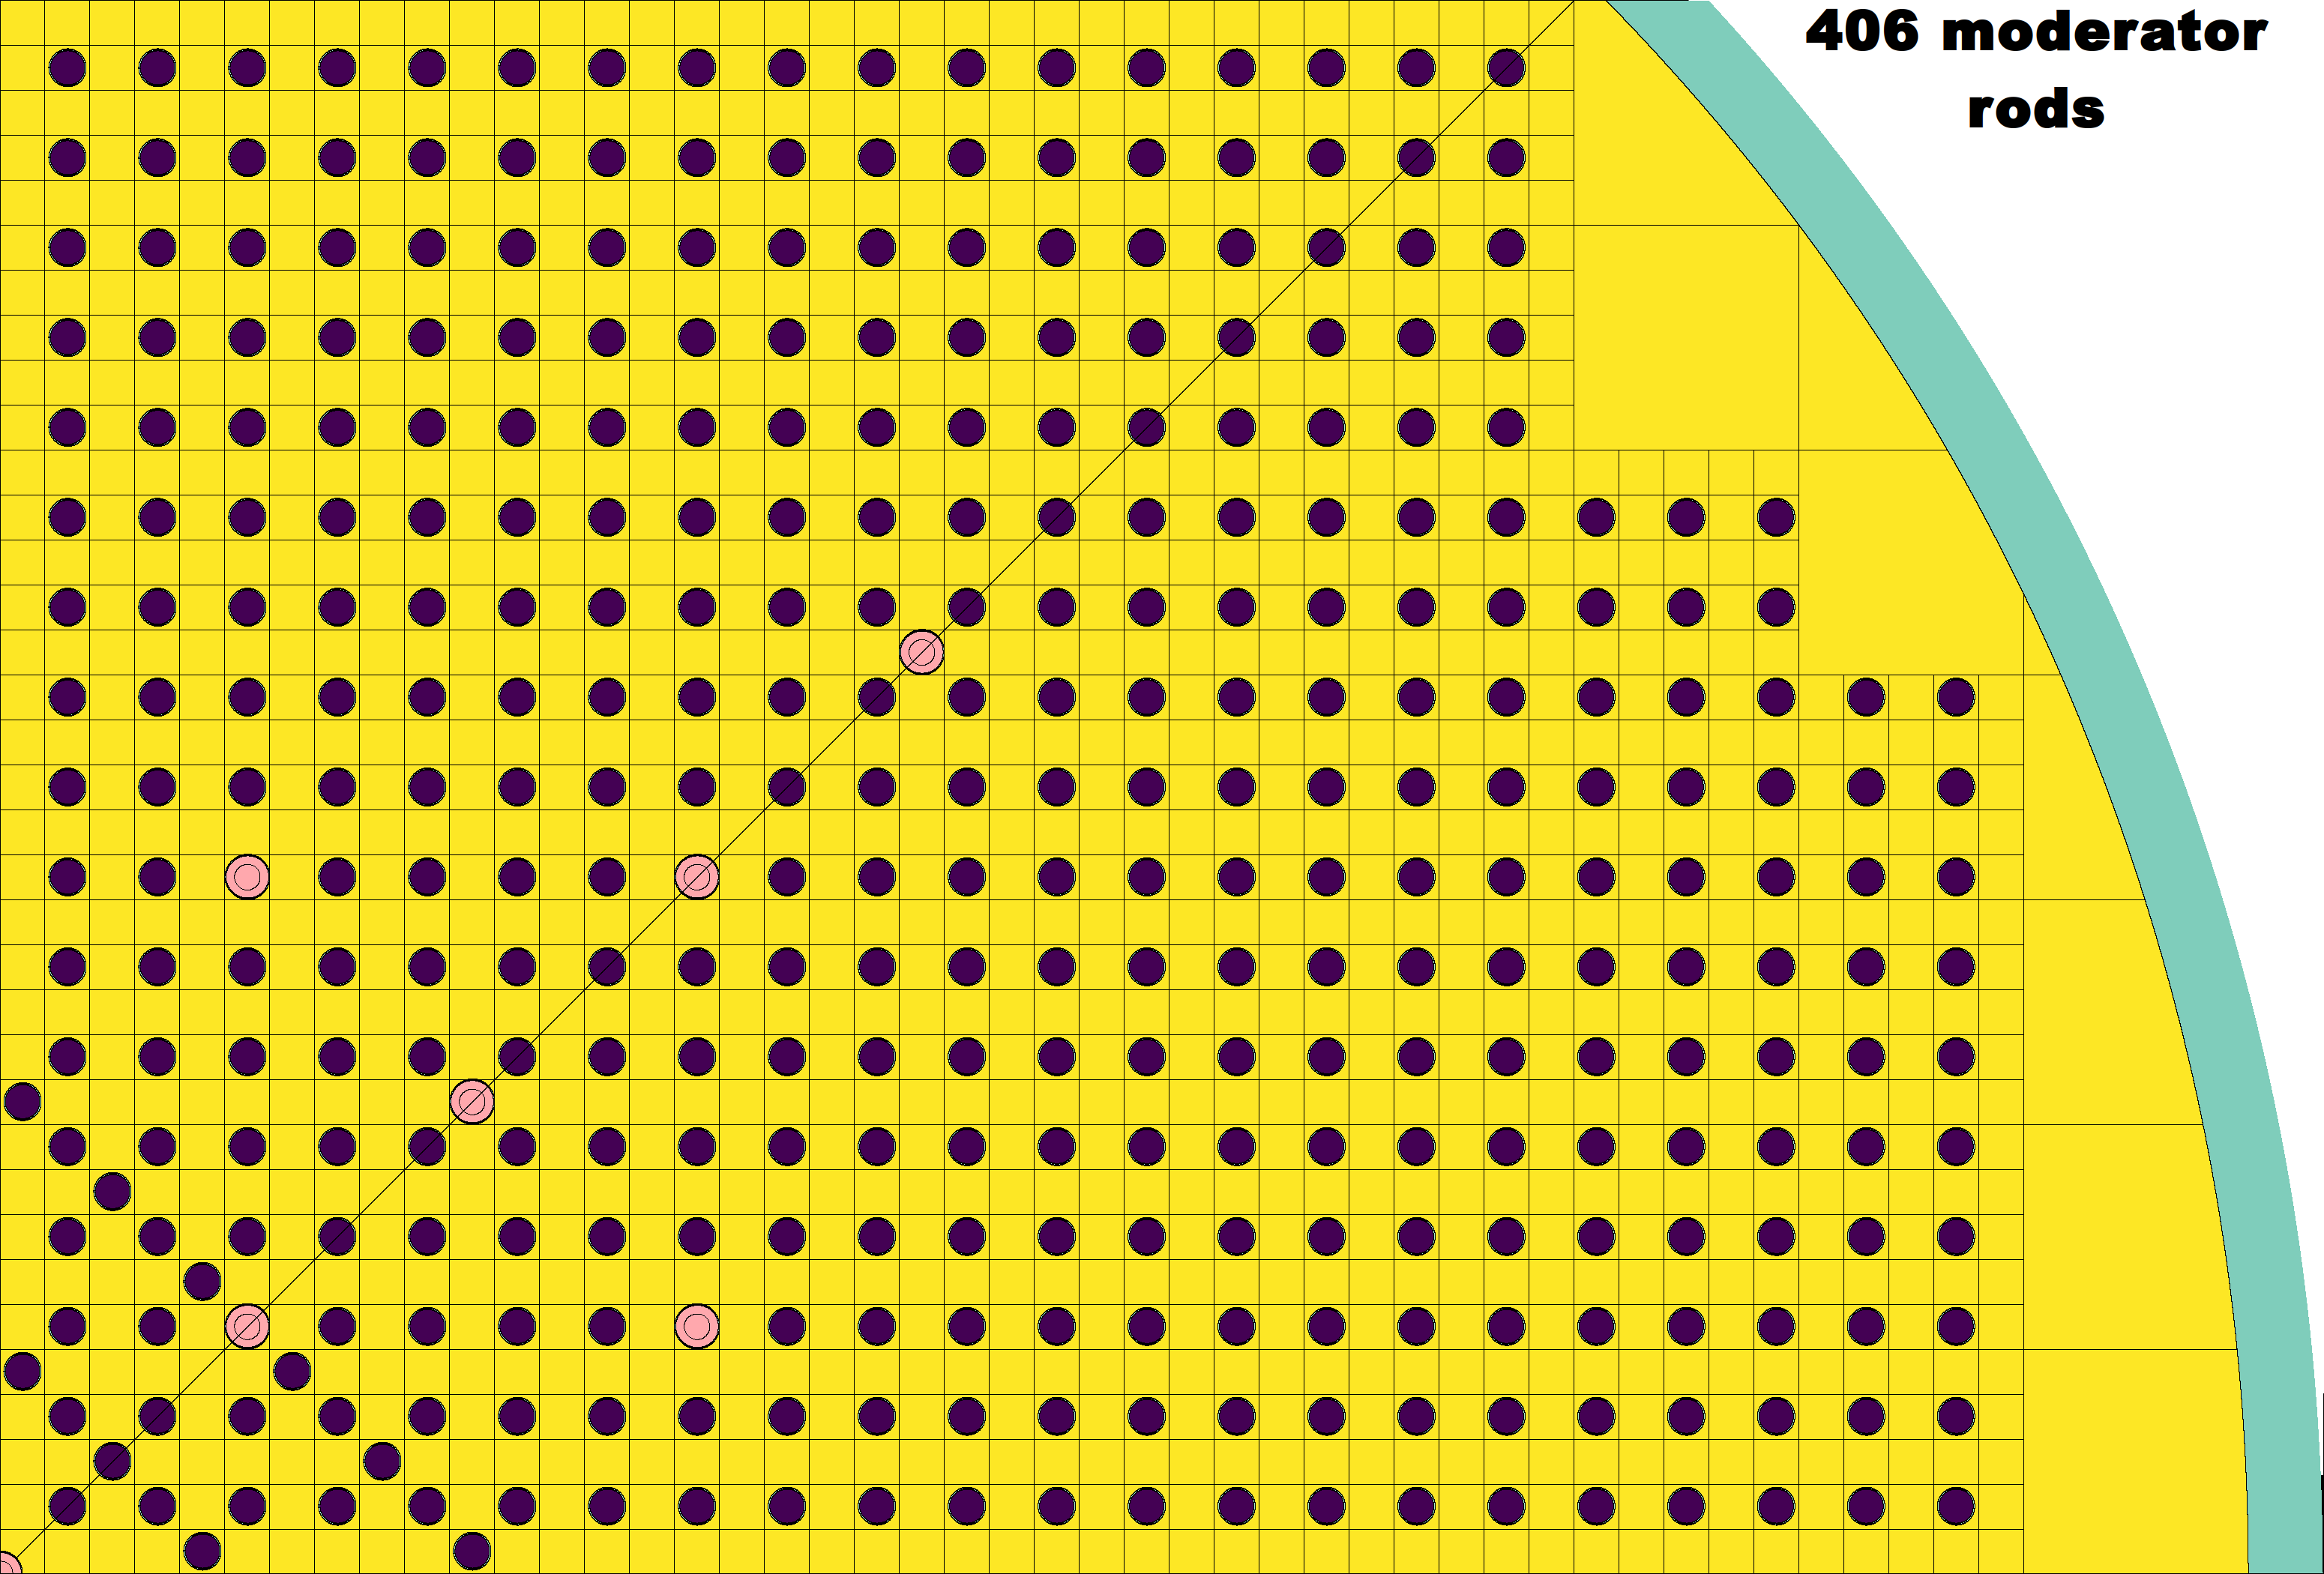
\includegraphics[height=0.75\textheight]{./images/406.png}}
		\onslide<3>\centerline{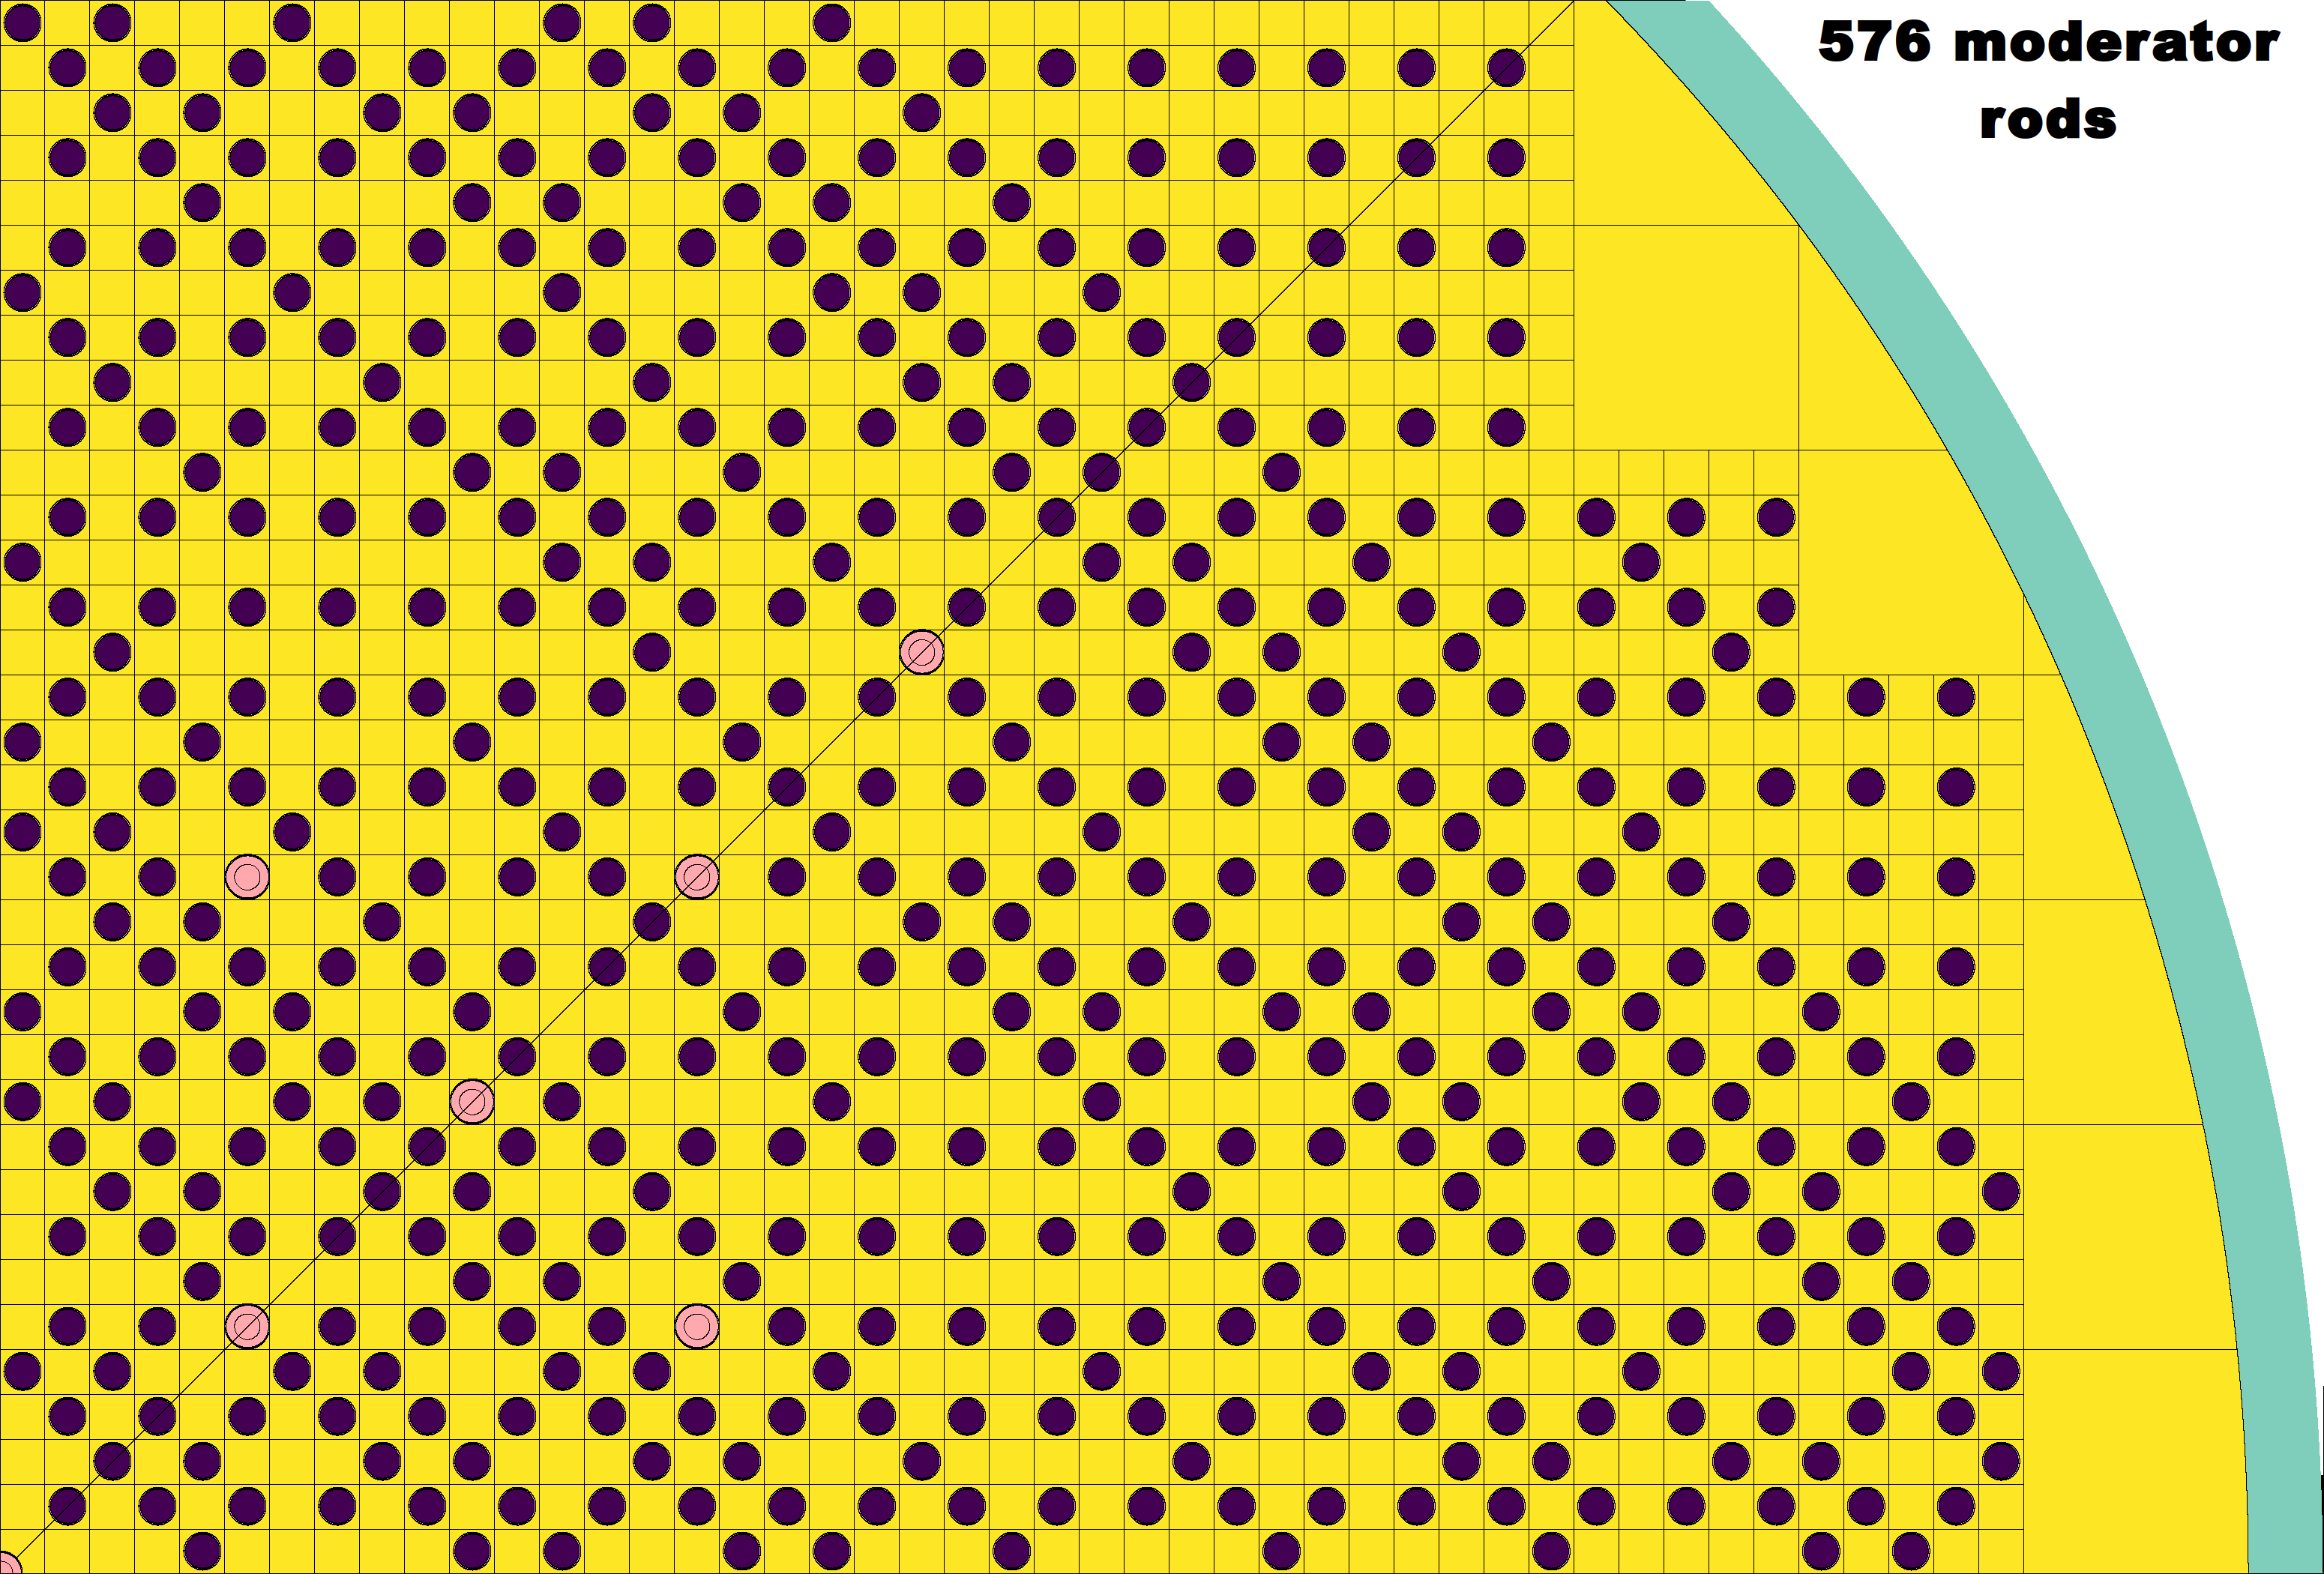
\includegraphics[height=0.75\textheight]{./images/576.png}}
		\onslide<4>\centerline{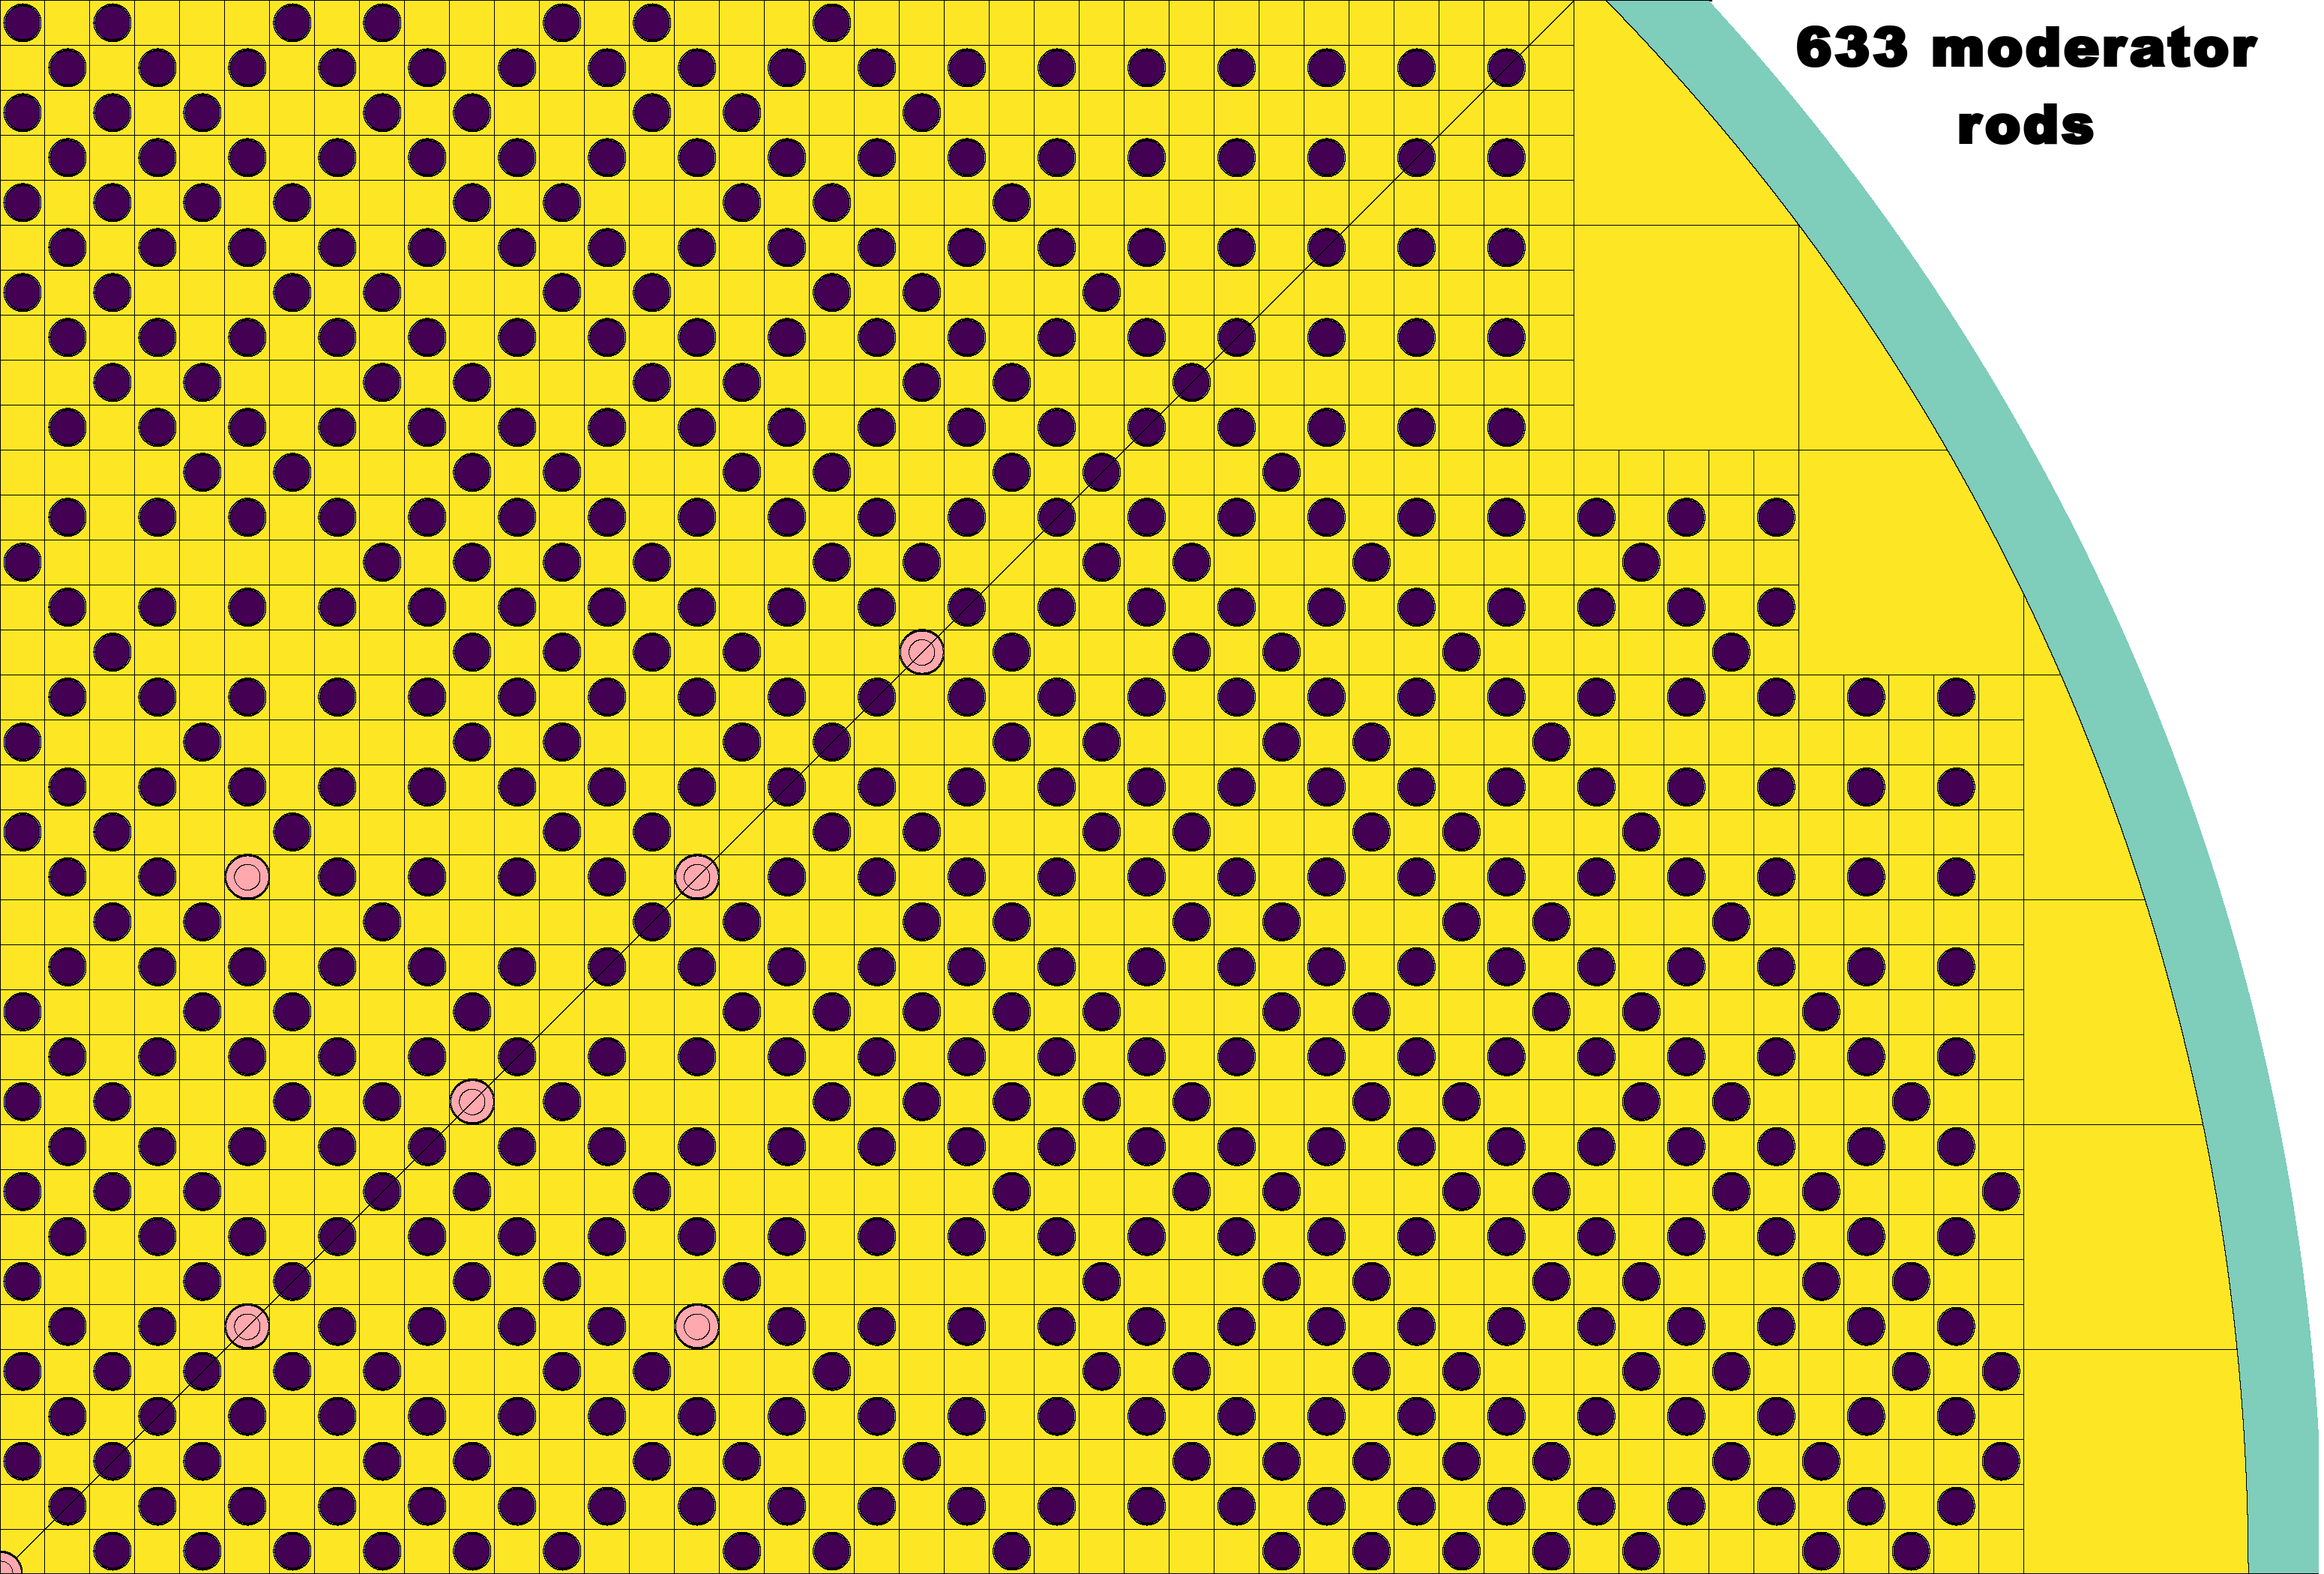
\includegraphics[height=0.75\textheight]{./images/633.png}}
		\onslide<5>\centerline{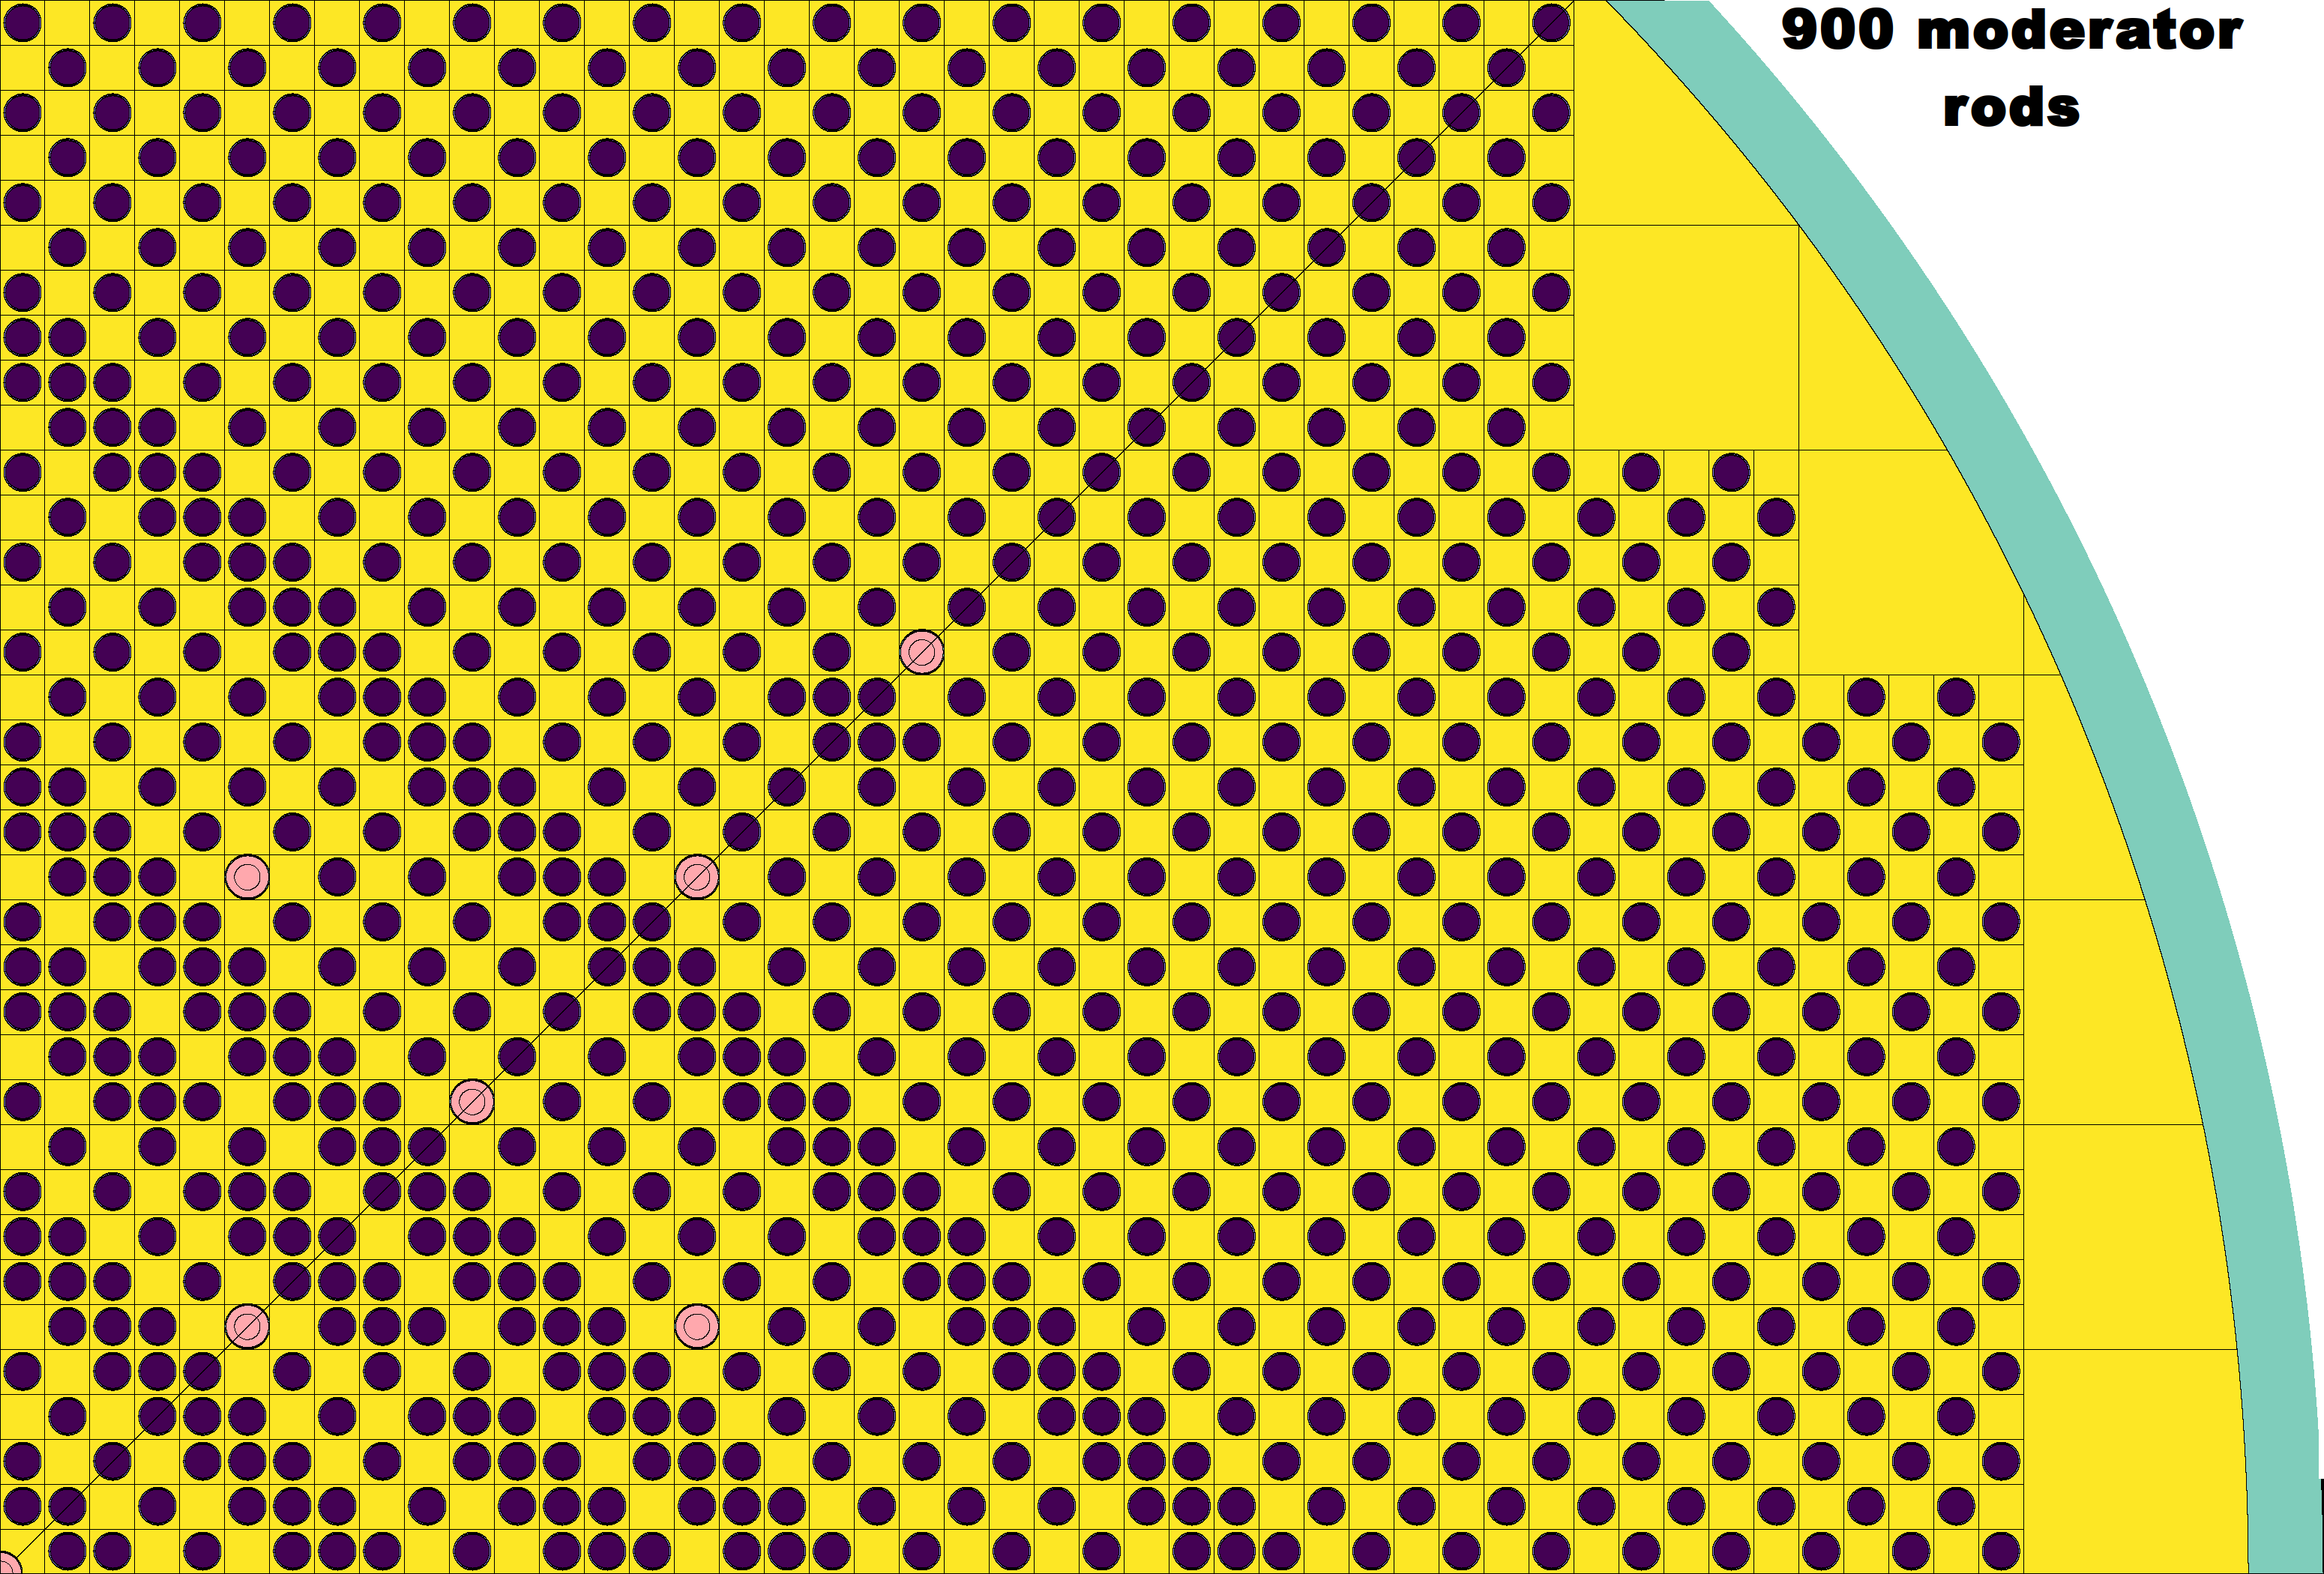
\includegraphics[height=0.75\textheight]{./images/900.png}}
		\onslide<6>\centerline{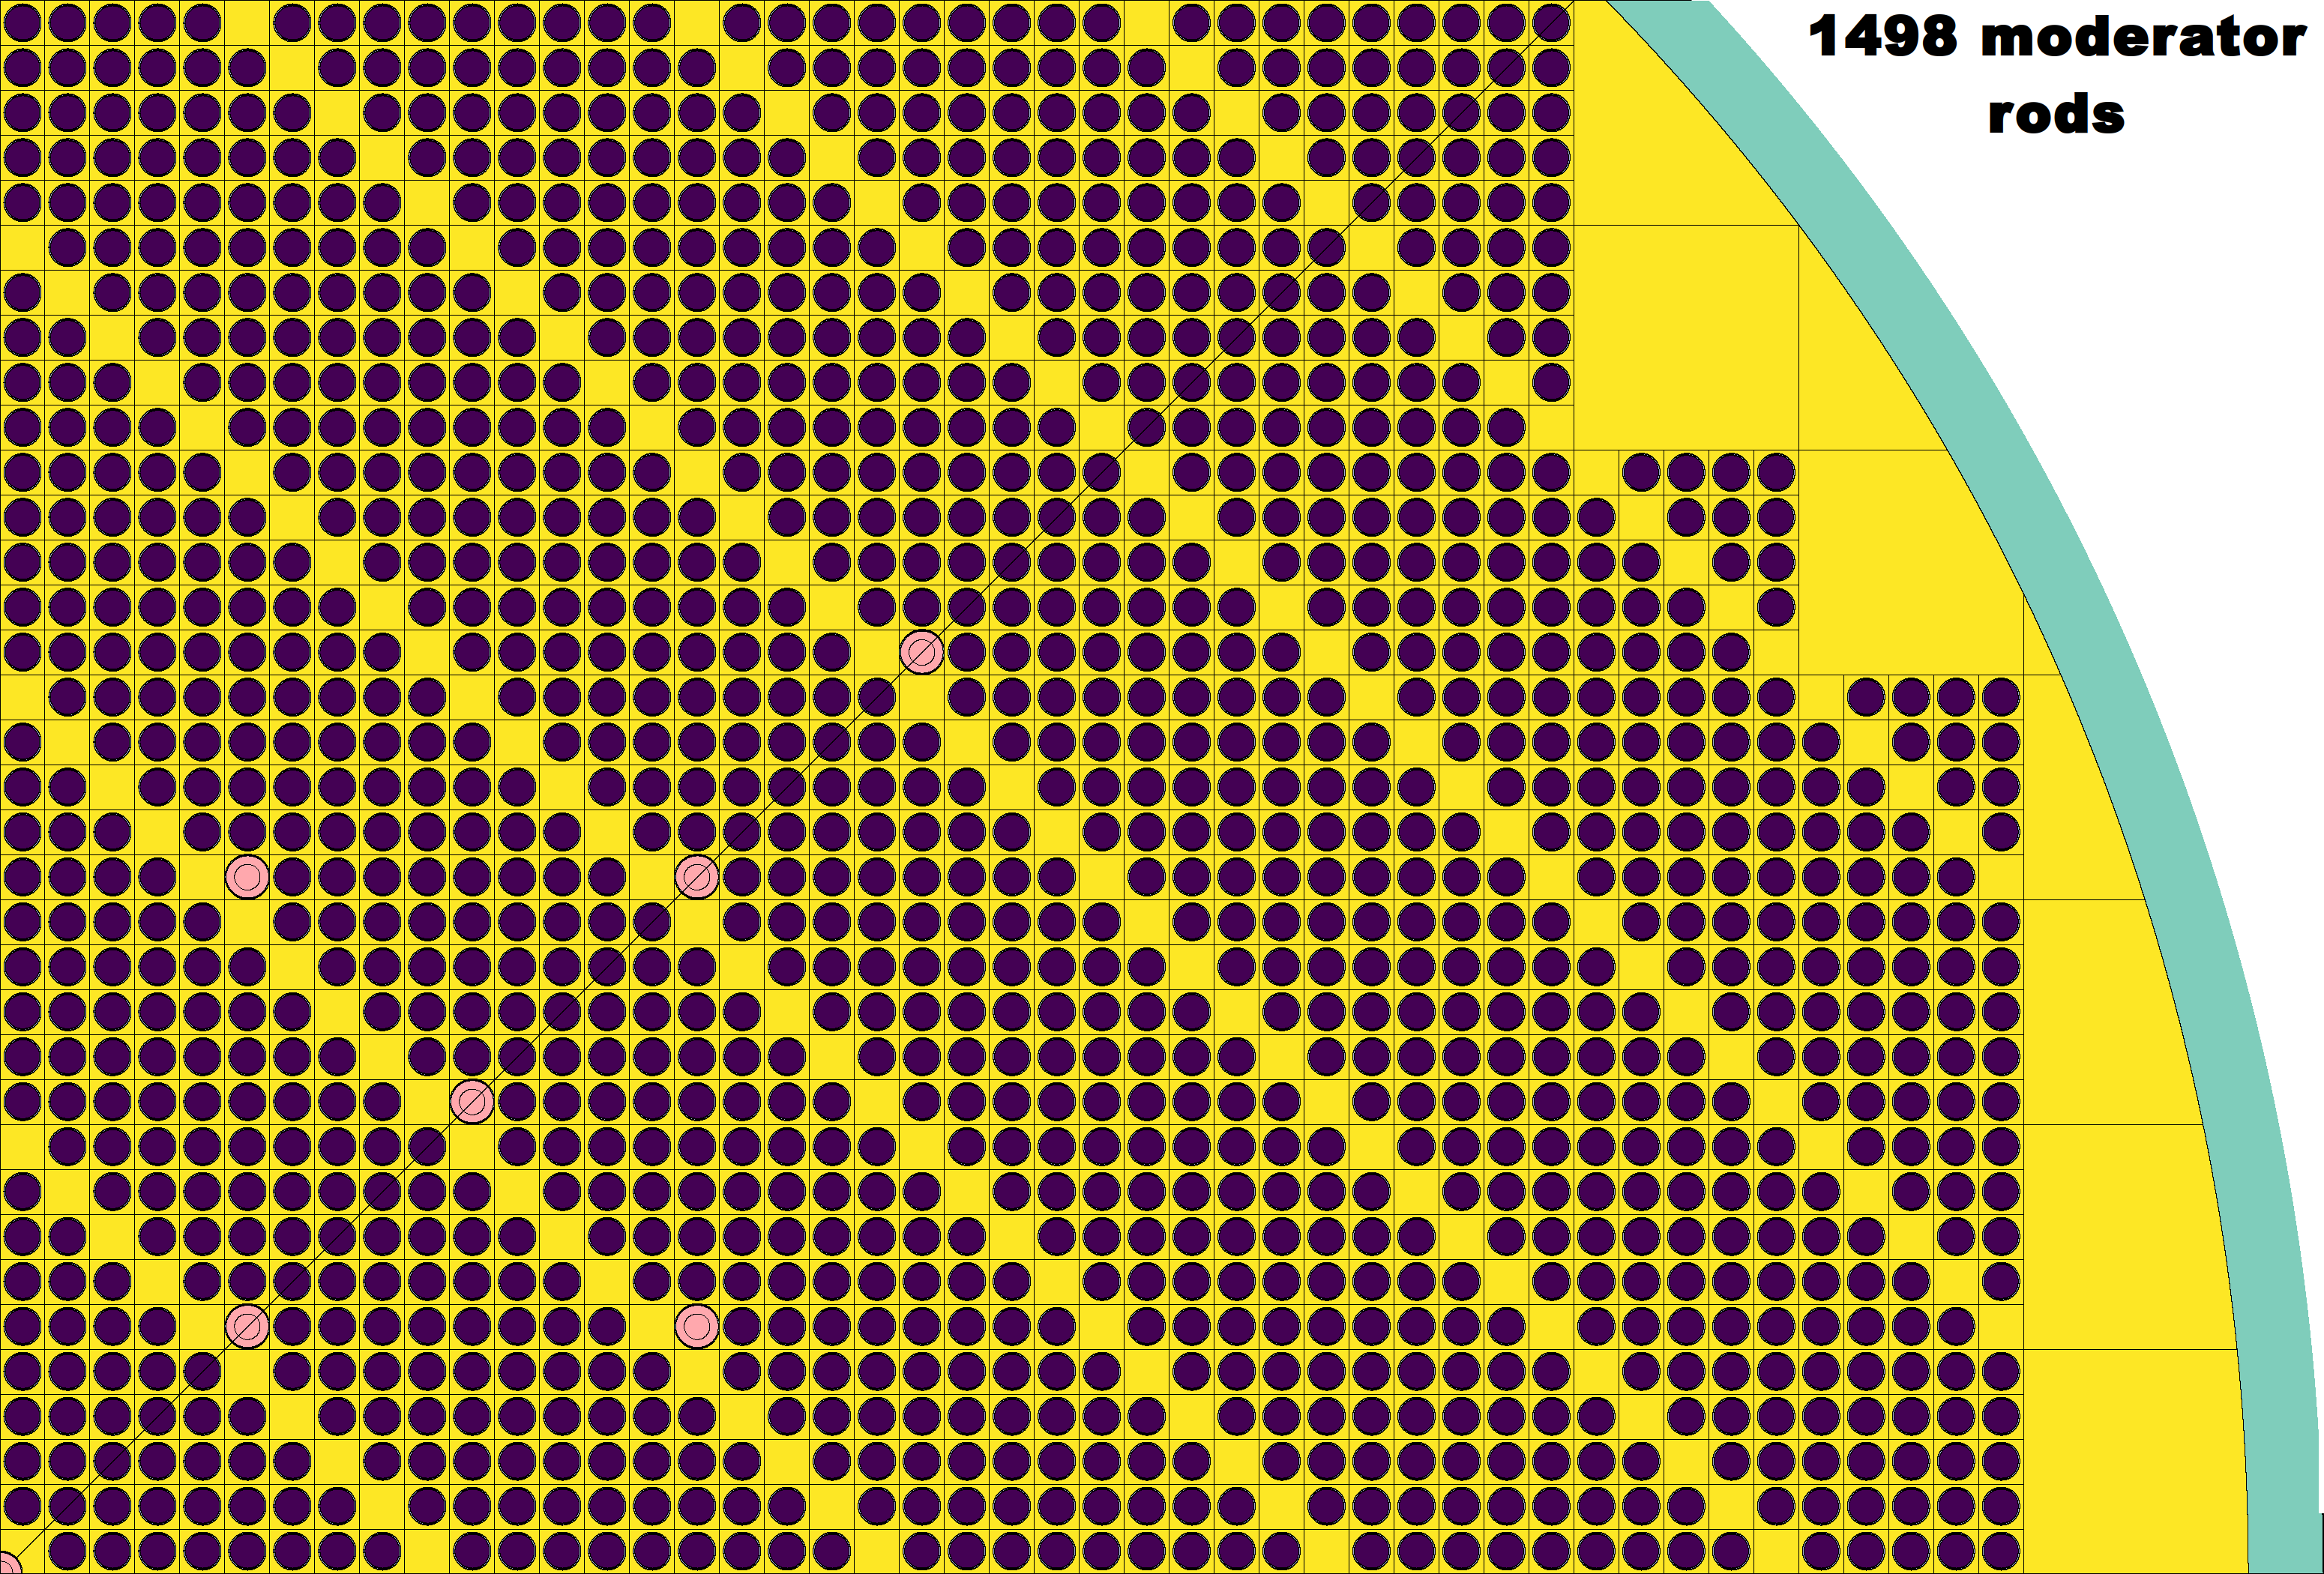
\includegraphics[height=0.75\textheight]{./images/1498.png}}
		\onslide<7>\centerline{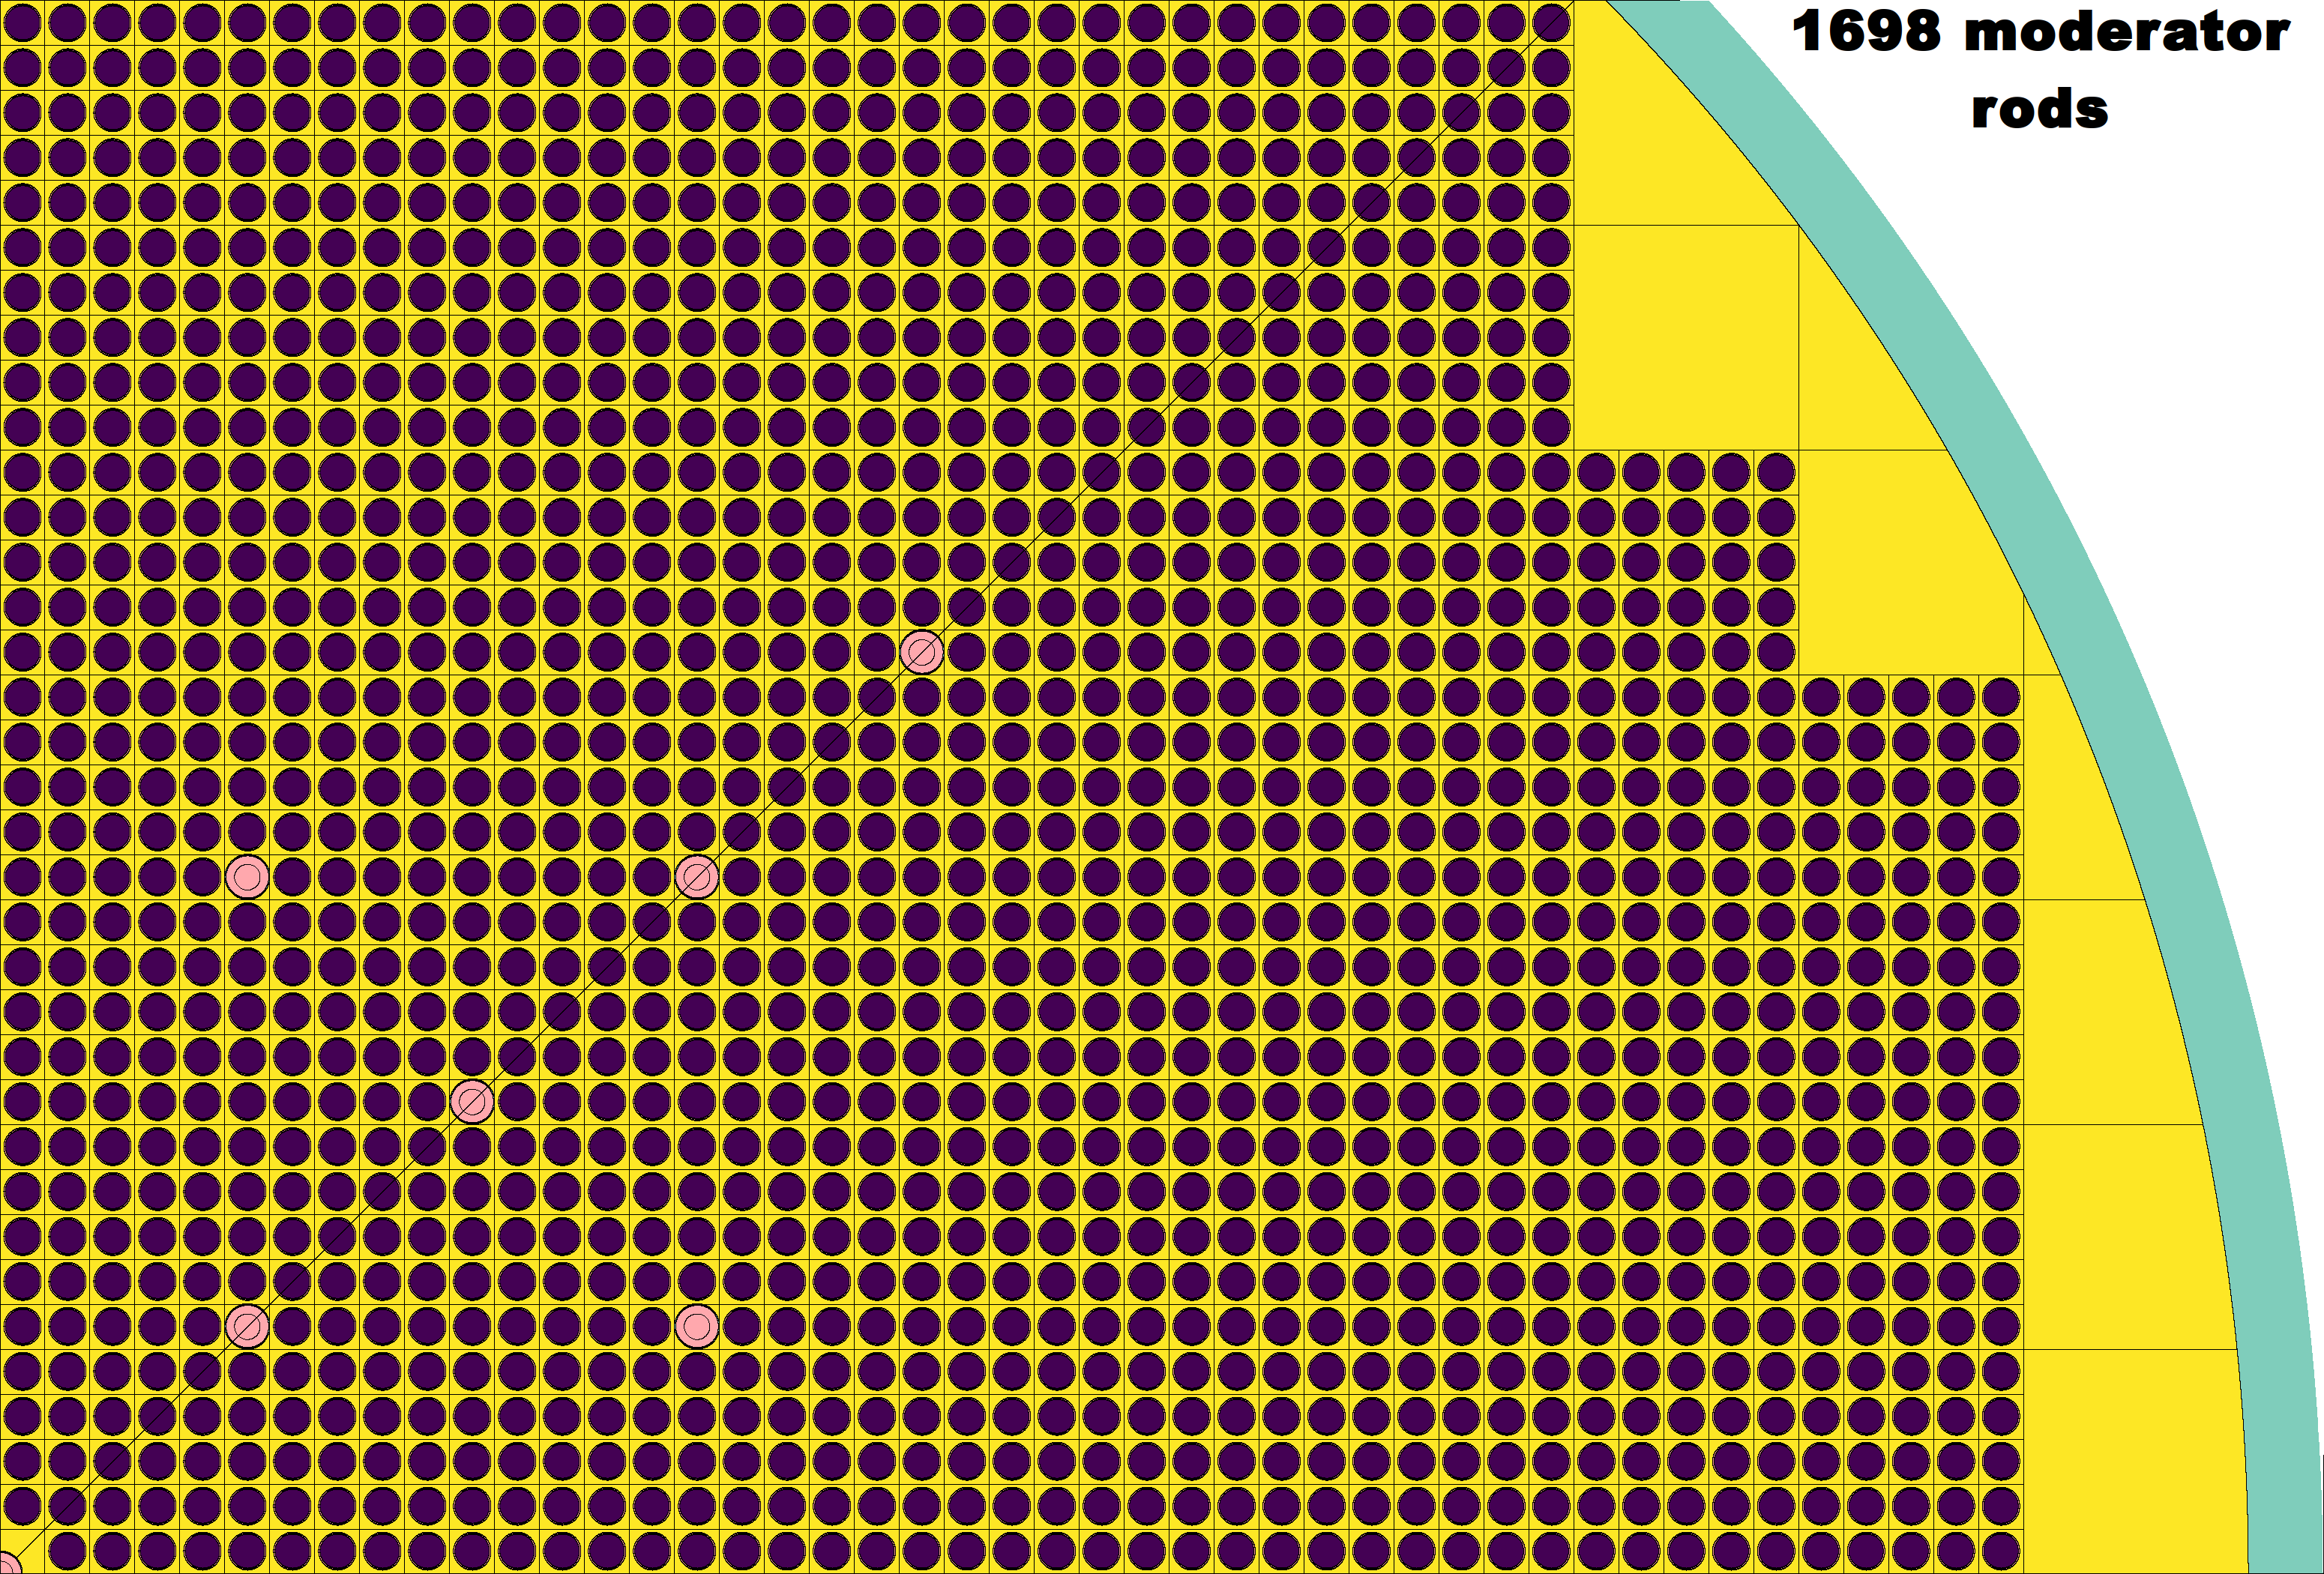
\includegraphics[height=0.75\textheight]{./images/1668.png}}
	\end{overprint}
	\caption{An $XY$ section of the \gls{TAP} model with various 
	moderator-to-fuel ratio. The violet color represents zirconium hydride, 
	the yellow represents fuel 
		salt.}
\end{figure}
\end{textblock*}
\end{frame}



\begin{frame}
\frametitle{$k_{eff}$ dynamics during 23.5 years of TAP operation}
\vspace{-3mm}
\begin{columns}
	\column{4.3cm}
	\begin{block}{Analysis assumptions}
		\fontsize{7}{9}\selectfont
		\begin{itemize}
			\item Quarter-core Serpent model
			\item Fine depletion resolution (\textbf{3-day})
			\item Xe removal efficiency $\epsilon_{Xe}=$\textcolor{green}{
			0.03}, \textcolor{orange}{0.54}, and \textcolor{blue}{0.92} for 
			mass transfer coefficient $K_L=$\textcolor{green}{0.085}, 
			\textcolor{orange}{2.117}, and \textcolor{blue}{8.467}$mm/s$
			\item 5\% LEU feed (UF$_4$) to maintain salt inventory
		\end{itemize}
	\end{block}
	\vspace{-2mm}
	\begin{block}{Main findings}
		\fontsize{7}{9}\selectfont
		\begin{itemize}
			\item $^{235}$U is substituted with $^{239}$Pu
			\item Poisonous $^{234}$U is built-up ($>$1t at EOL)
			\item Total U inventory decreased from 137 to 129t
		\end{itemize}  
	\end{block}  	
	
	\column{8cm}
	\begin{figure}[ht!] 
		\begin{overprint}
			\onslide<1>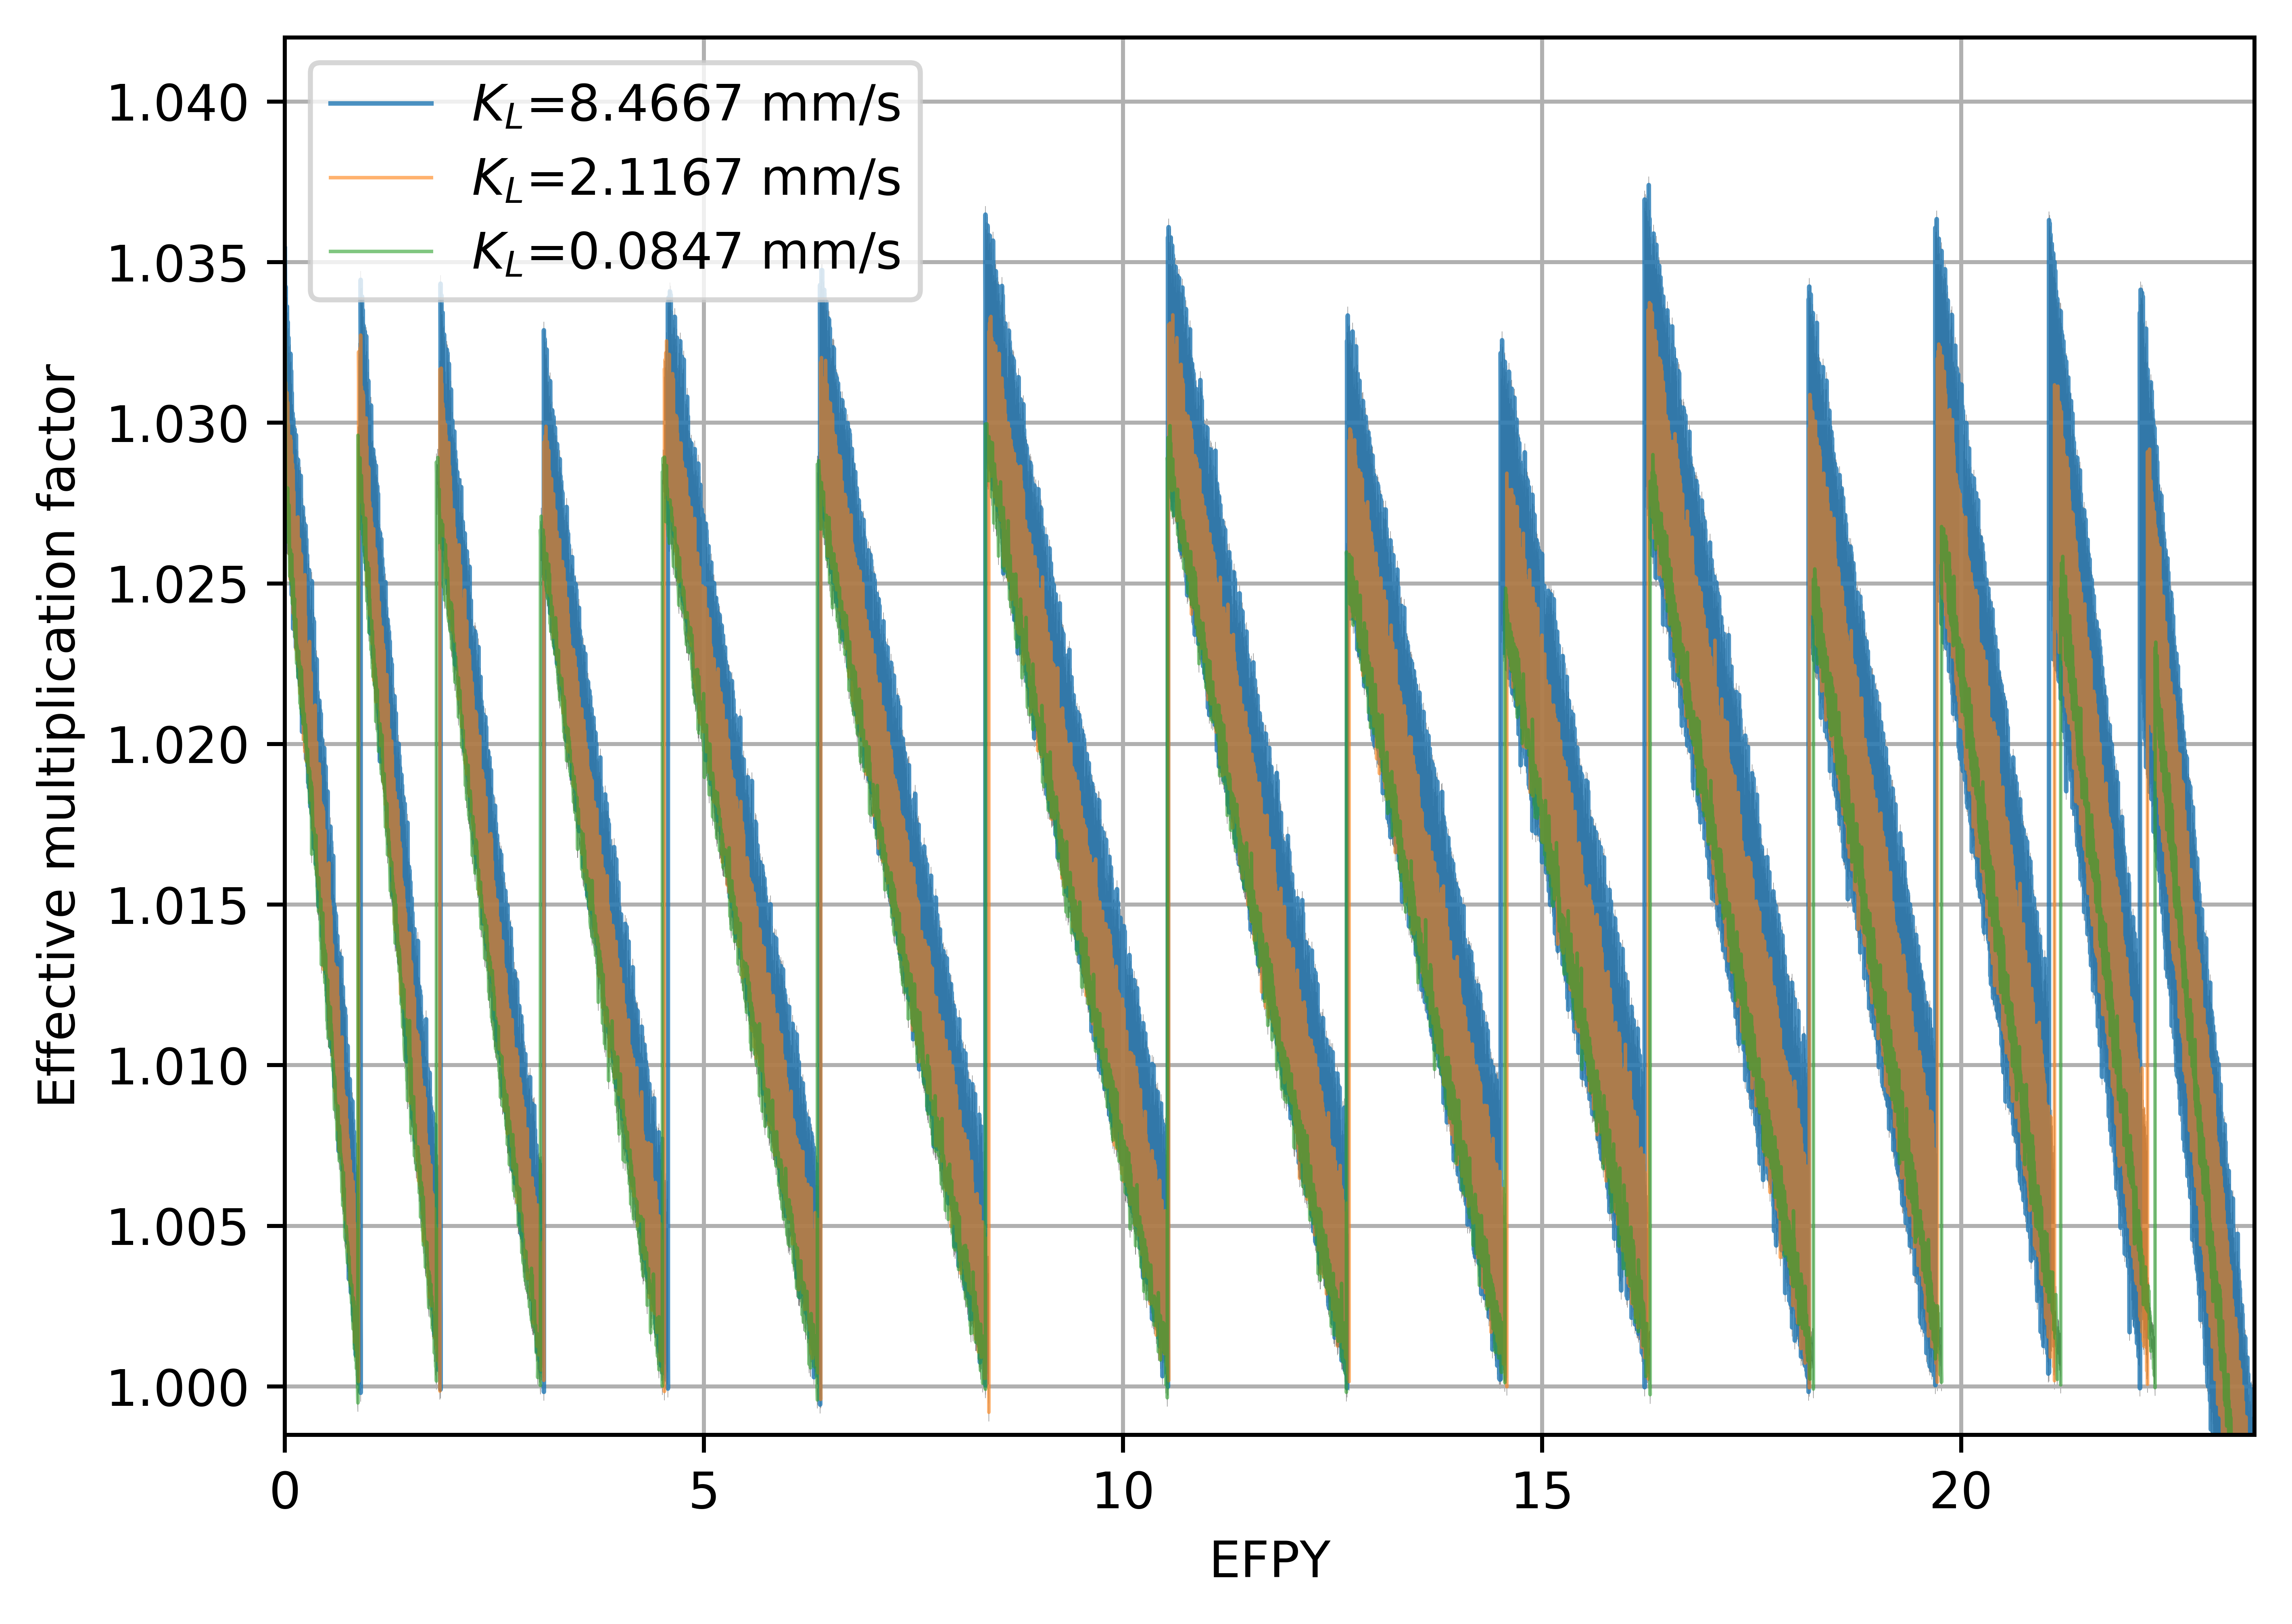
\includegraphics[width=\textwidth]{../dissertation/figures/ch4/eps/keff.png}
			\onslide<2>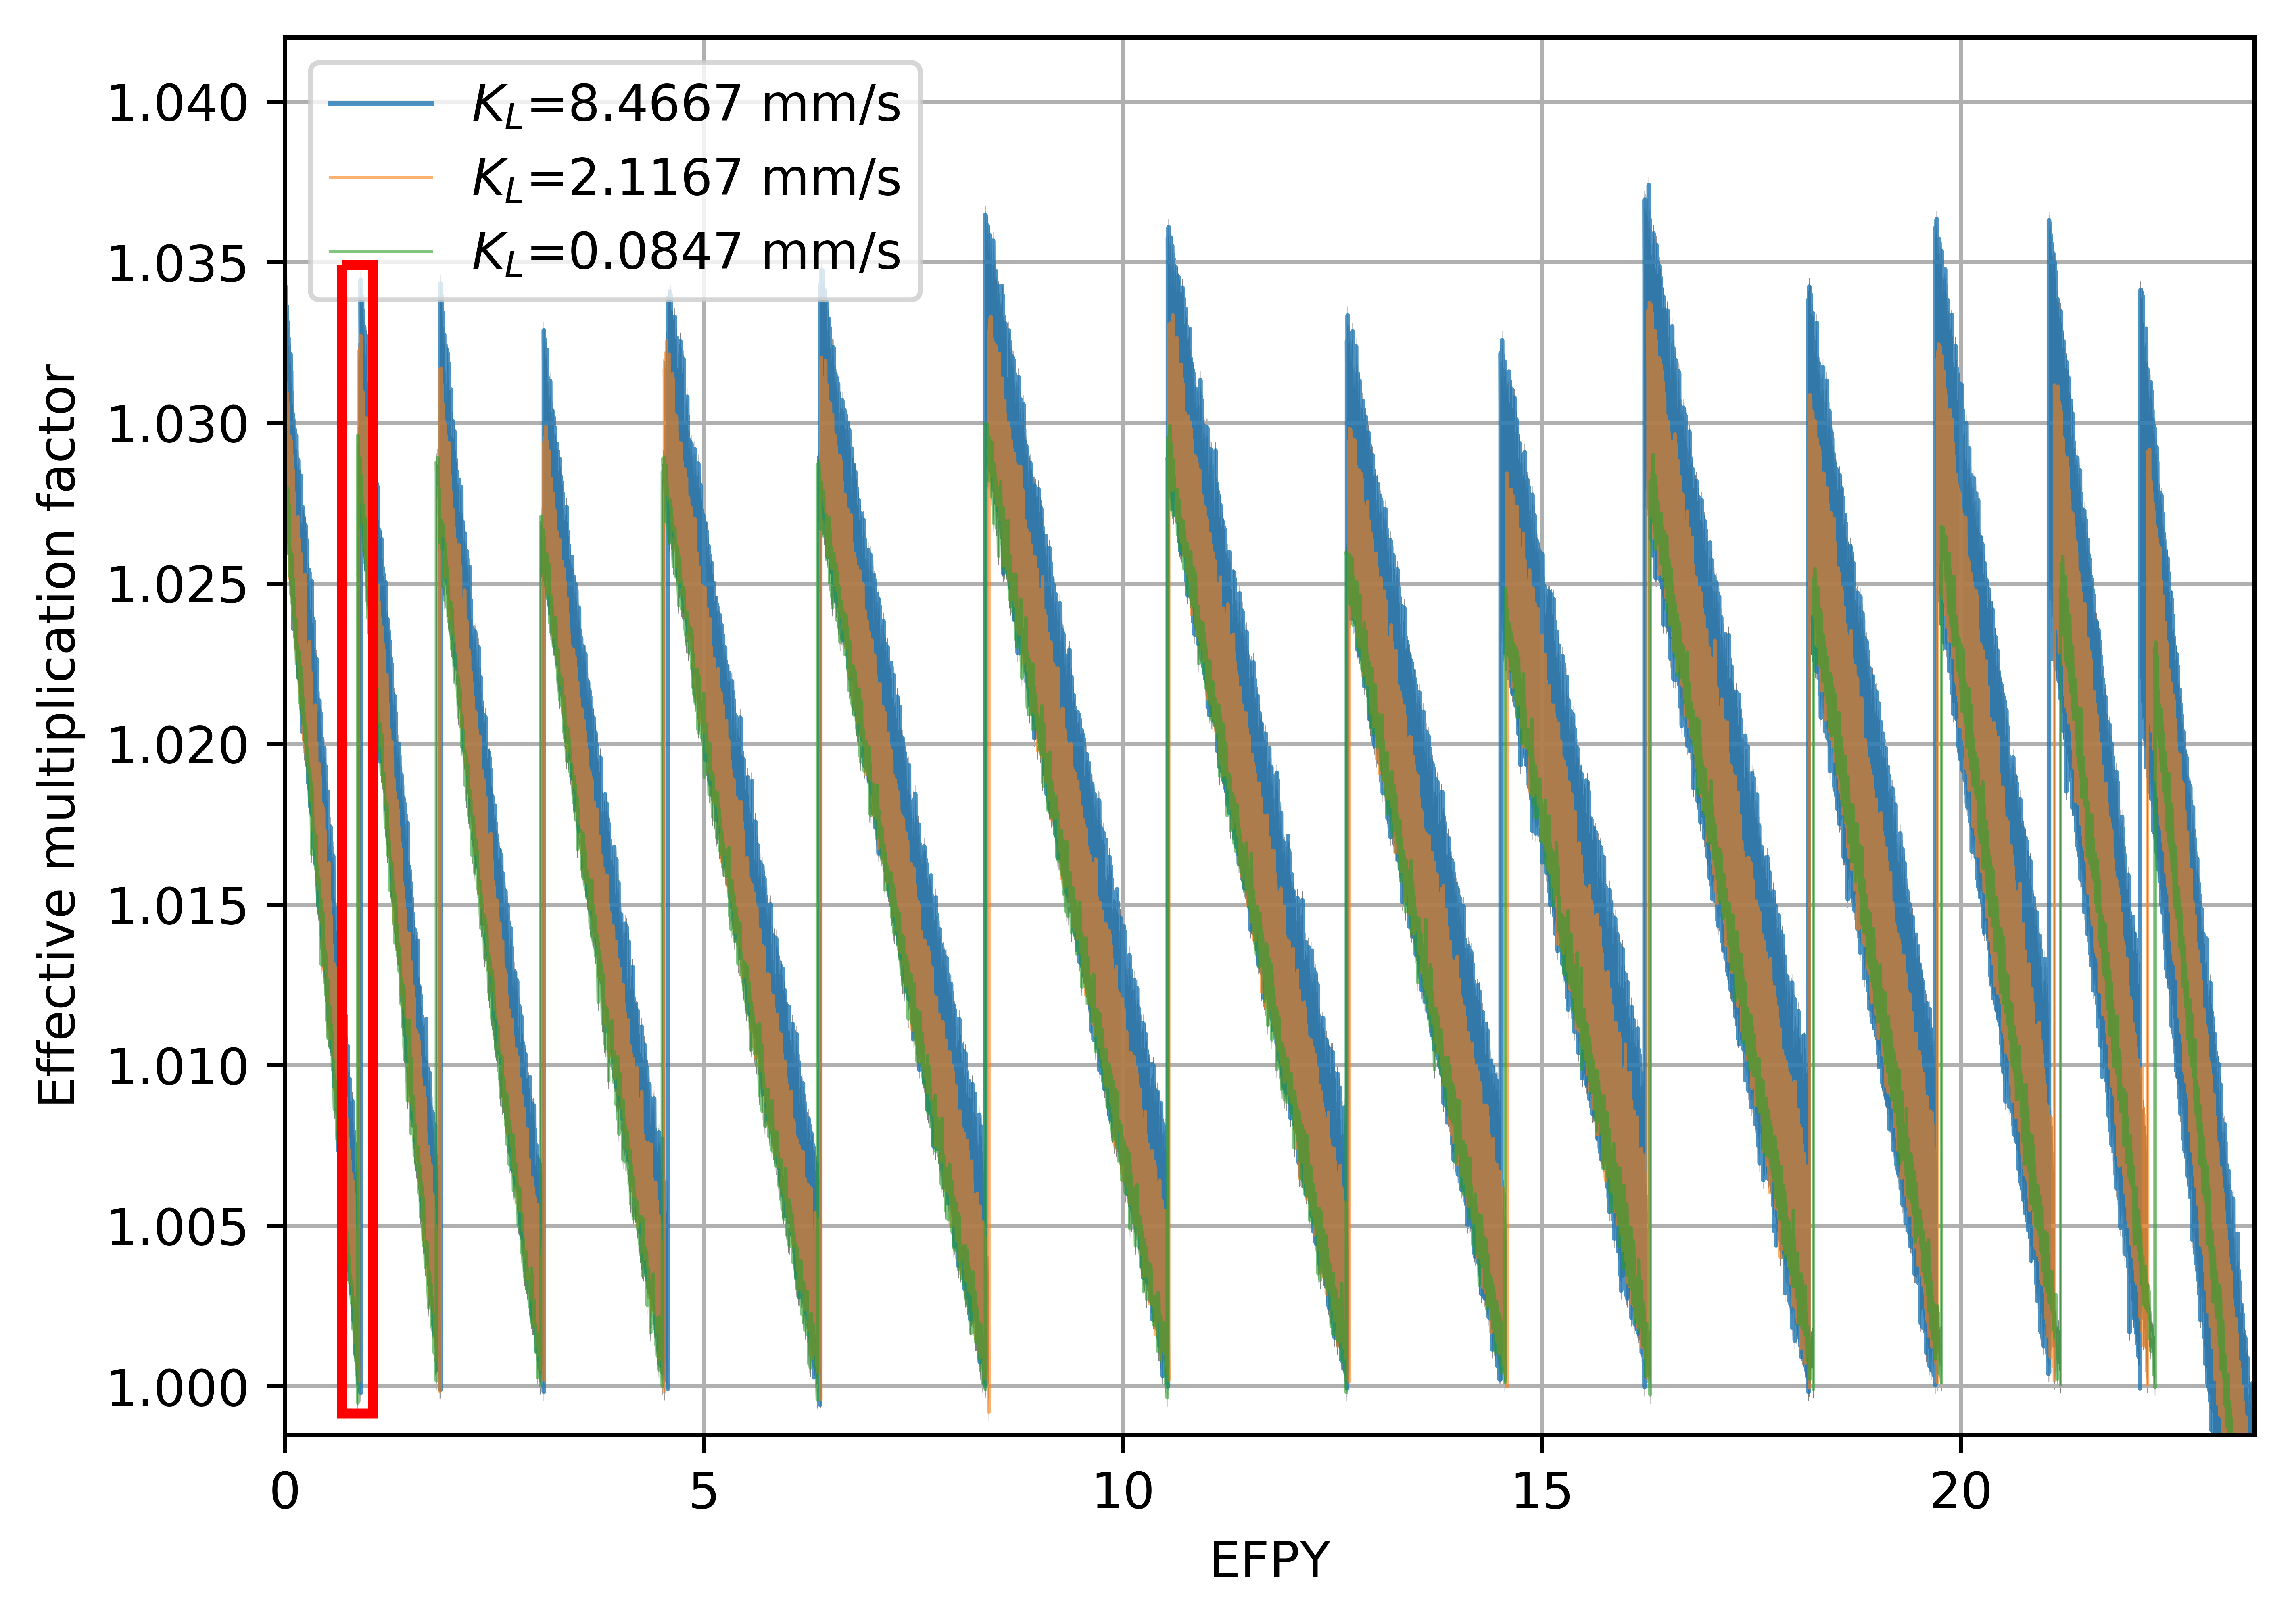
\includegraphics[width=\textwidth]{./images/keff_z_1.png}
			\onslide<3>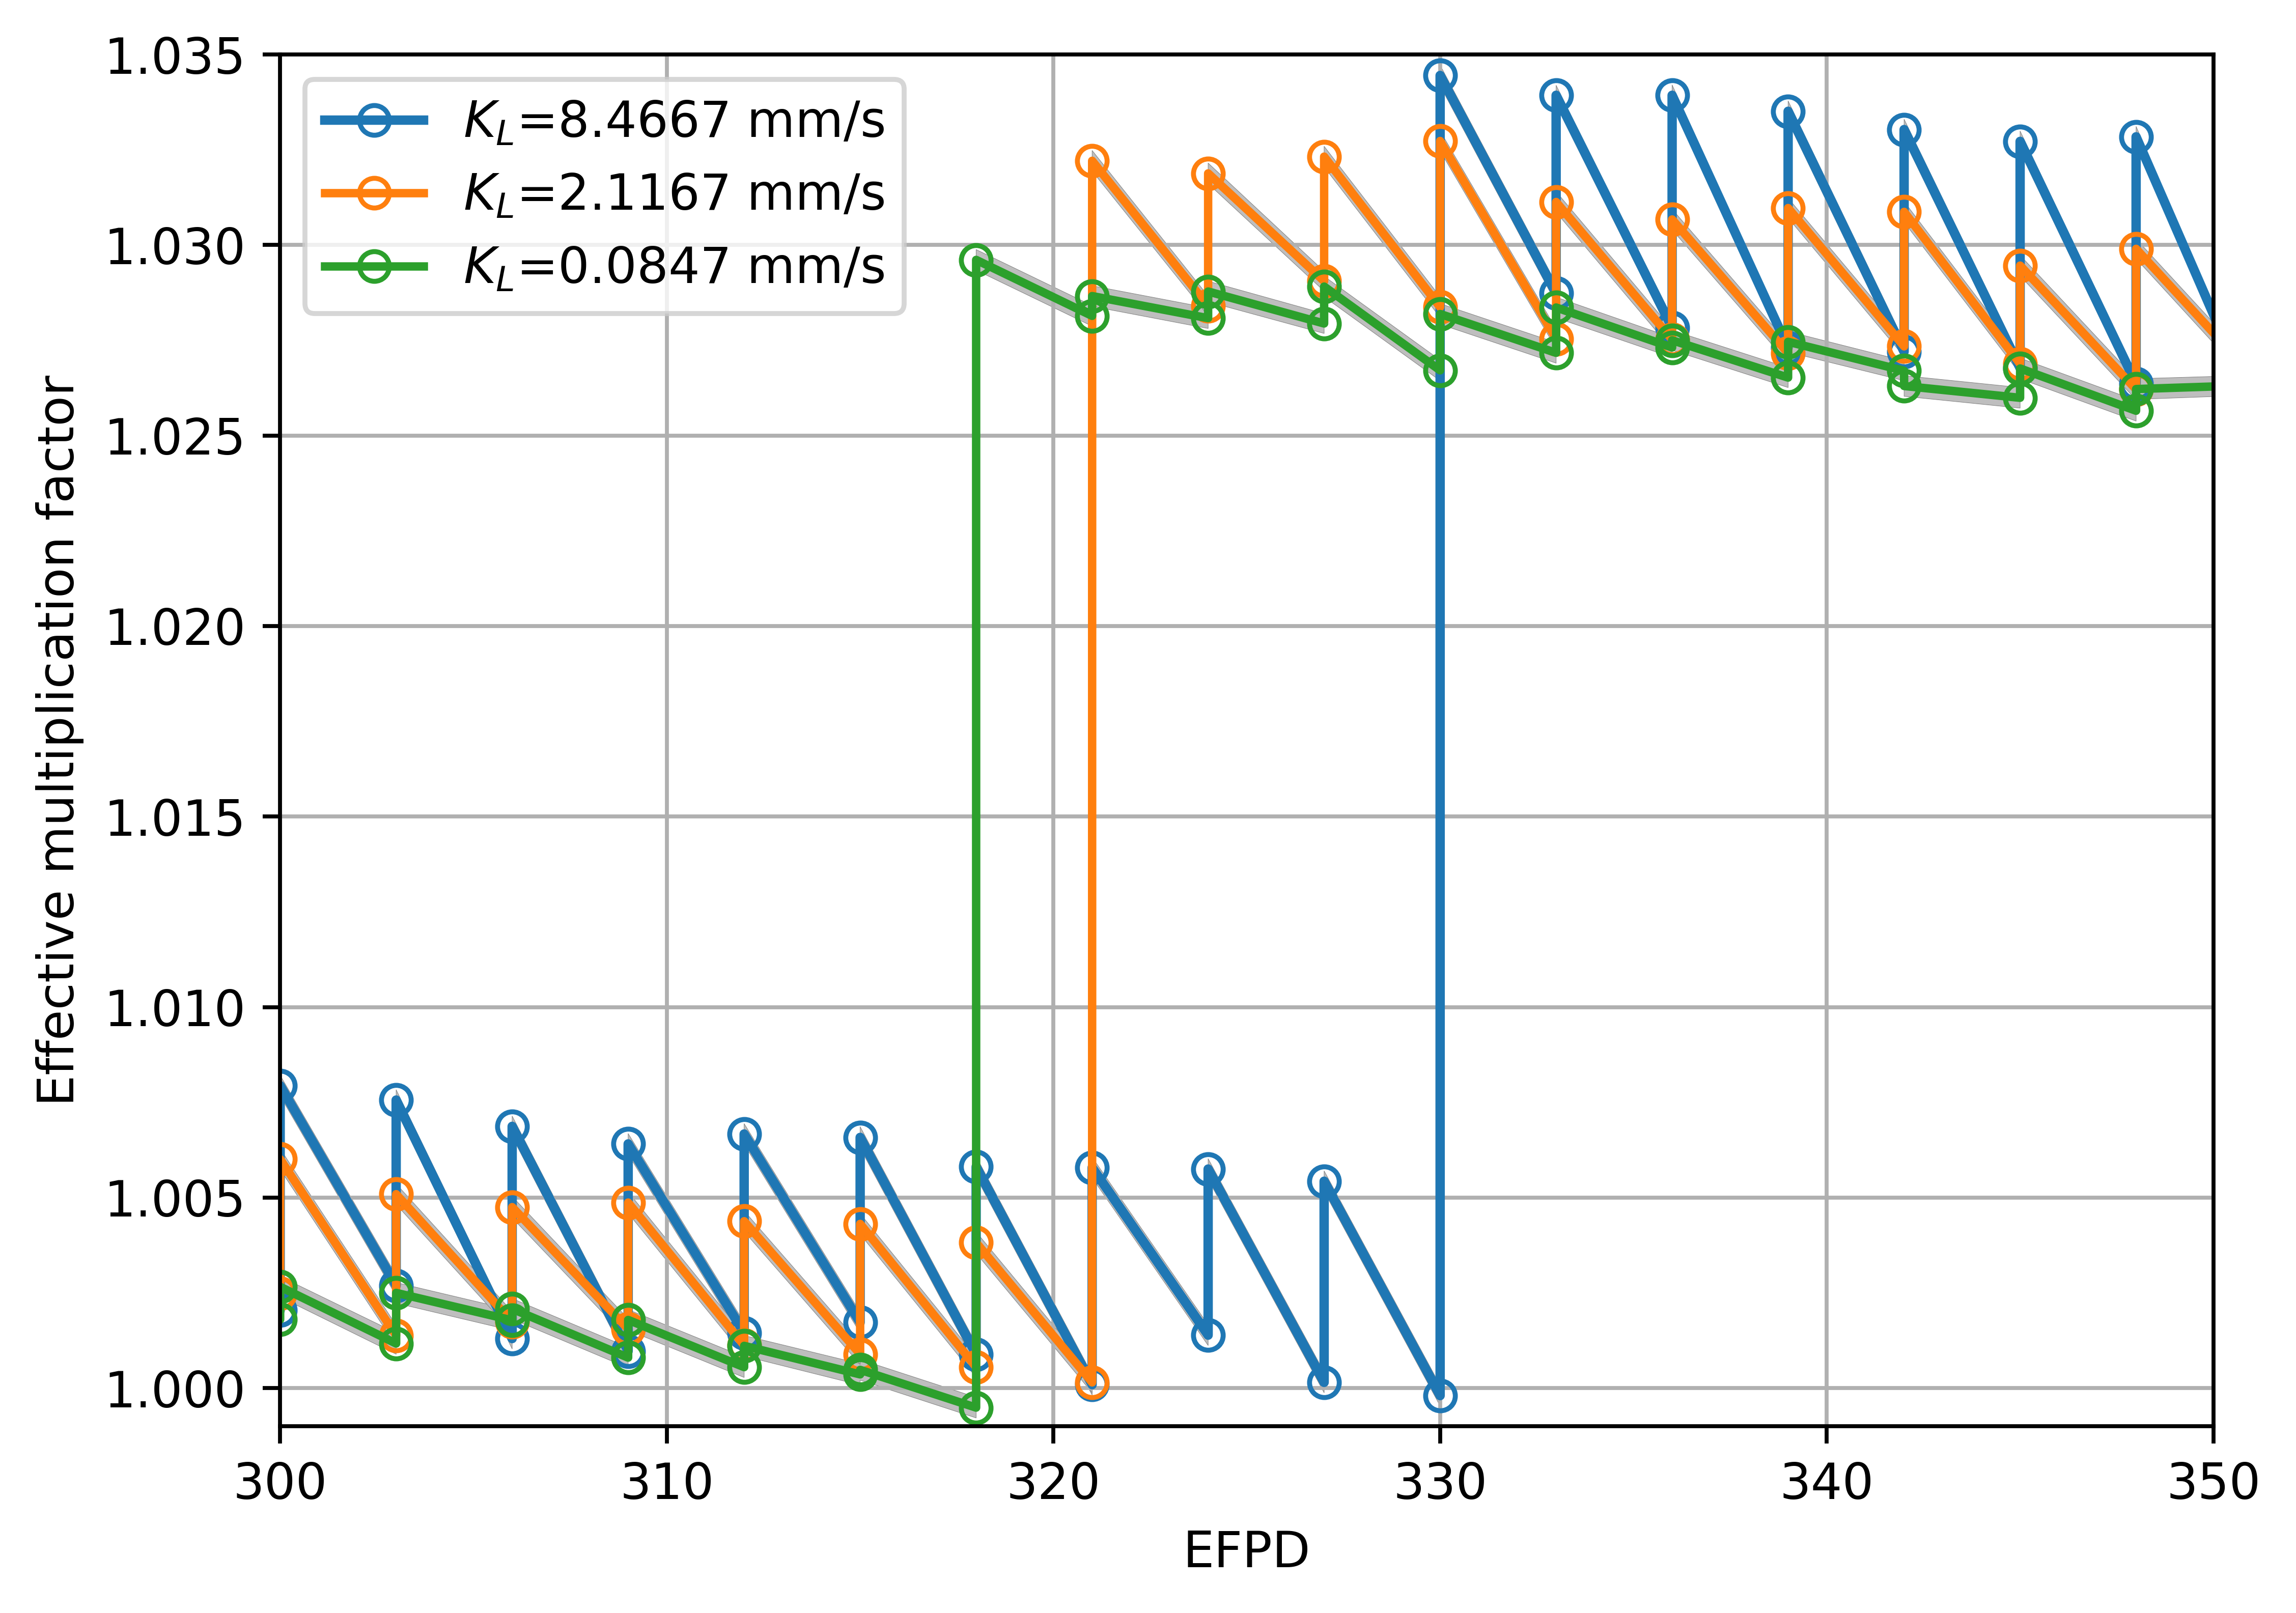
\includegraphics[width=\textwidth]{../dissertation/figures/ch4/eps/keff_zoomed_1.png}
			\vspace{-4mm}
		\end{overprint}
	\caption{SaltProc-calculated effective multiplication factor 
	for the full-core \gls{TAP} concept.}			
	\end{figure}
	
\end{columns}
\end{frame}


\begin{frame}
\frametitle{Neutron energy spectrum}
\begin{textblock*}{12.6cm}(0.1cm,1.7cm) % {block width} (coords)
	\begin{figure}[htp!] % replace 't' with 'b' to 
		\begin{overprint}
\onslide<1>\centerline{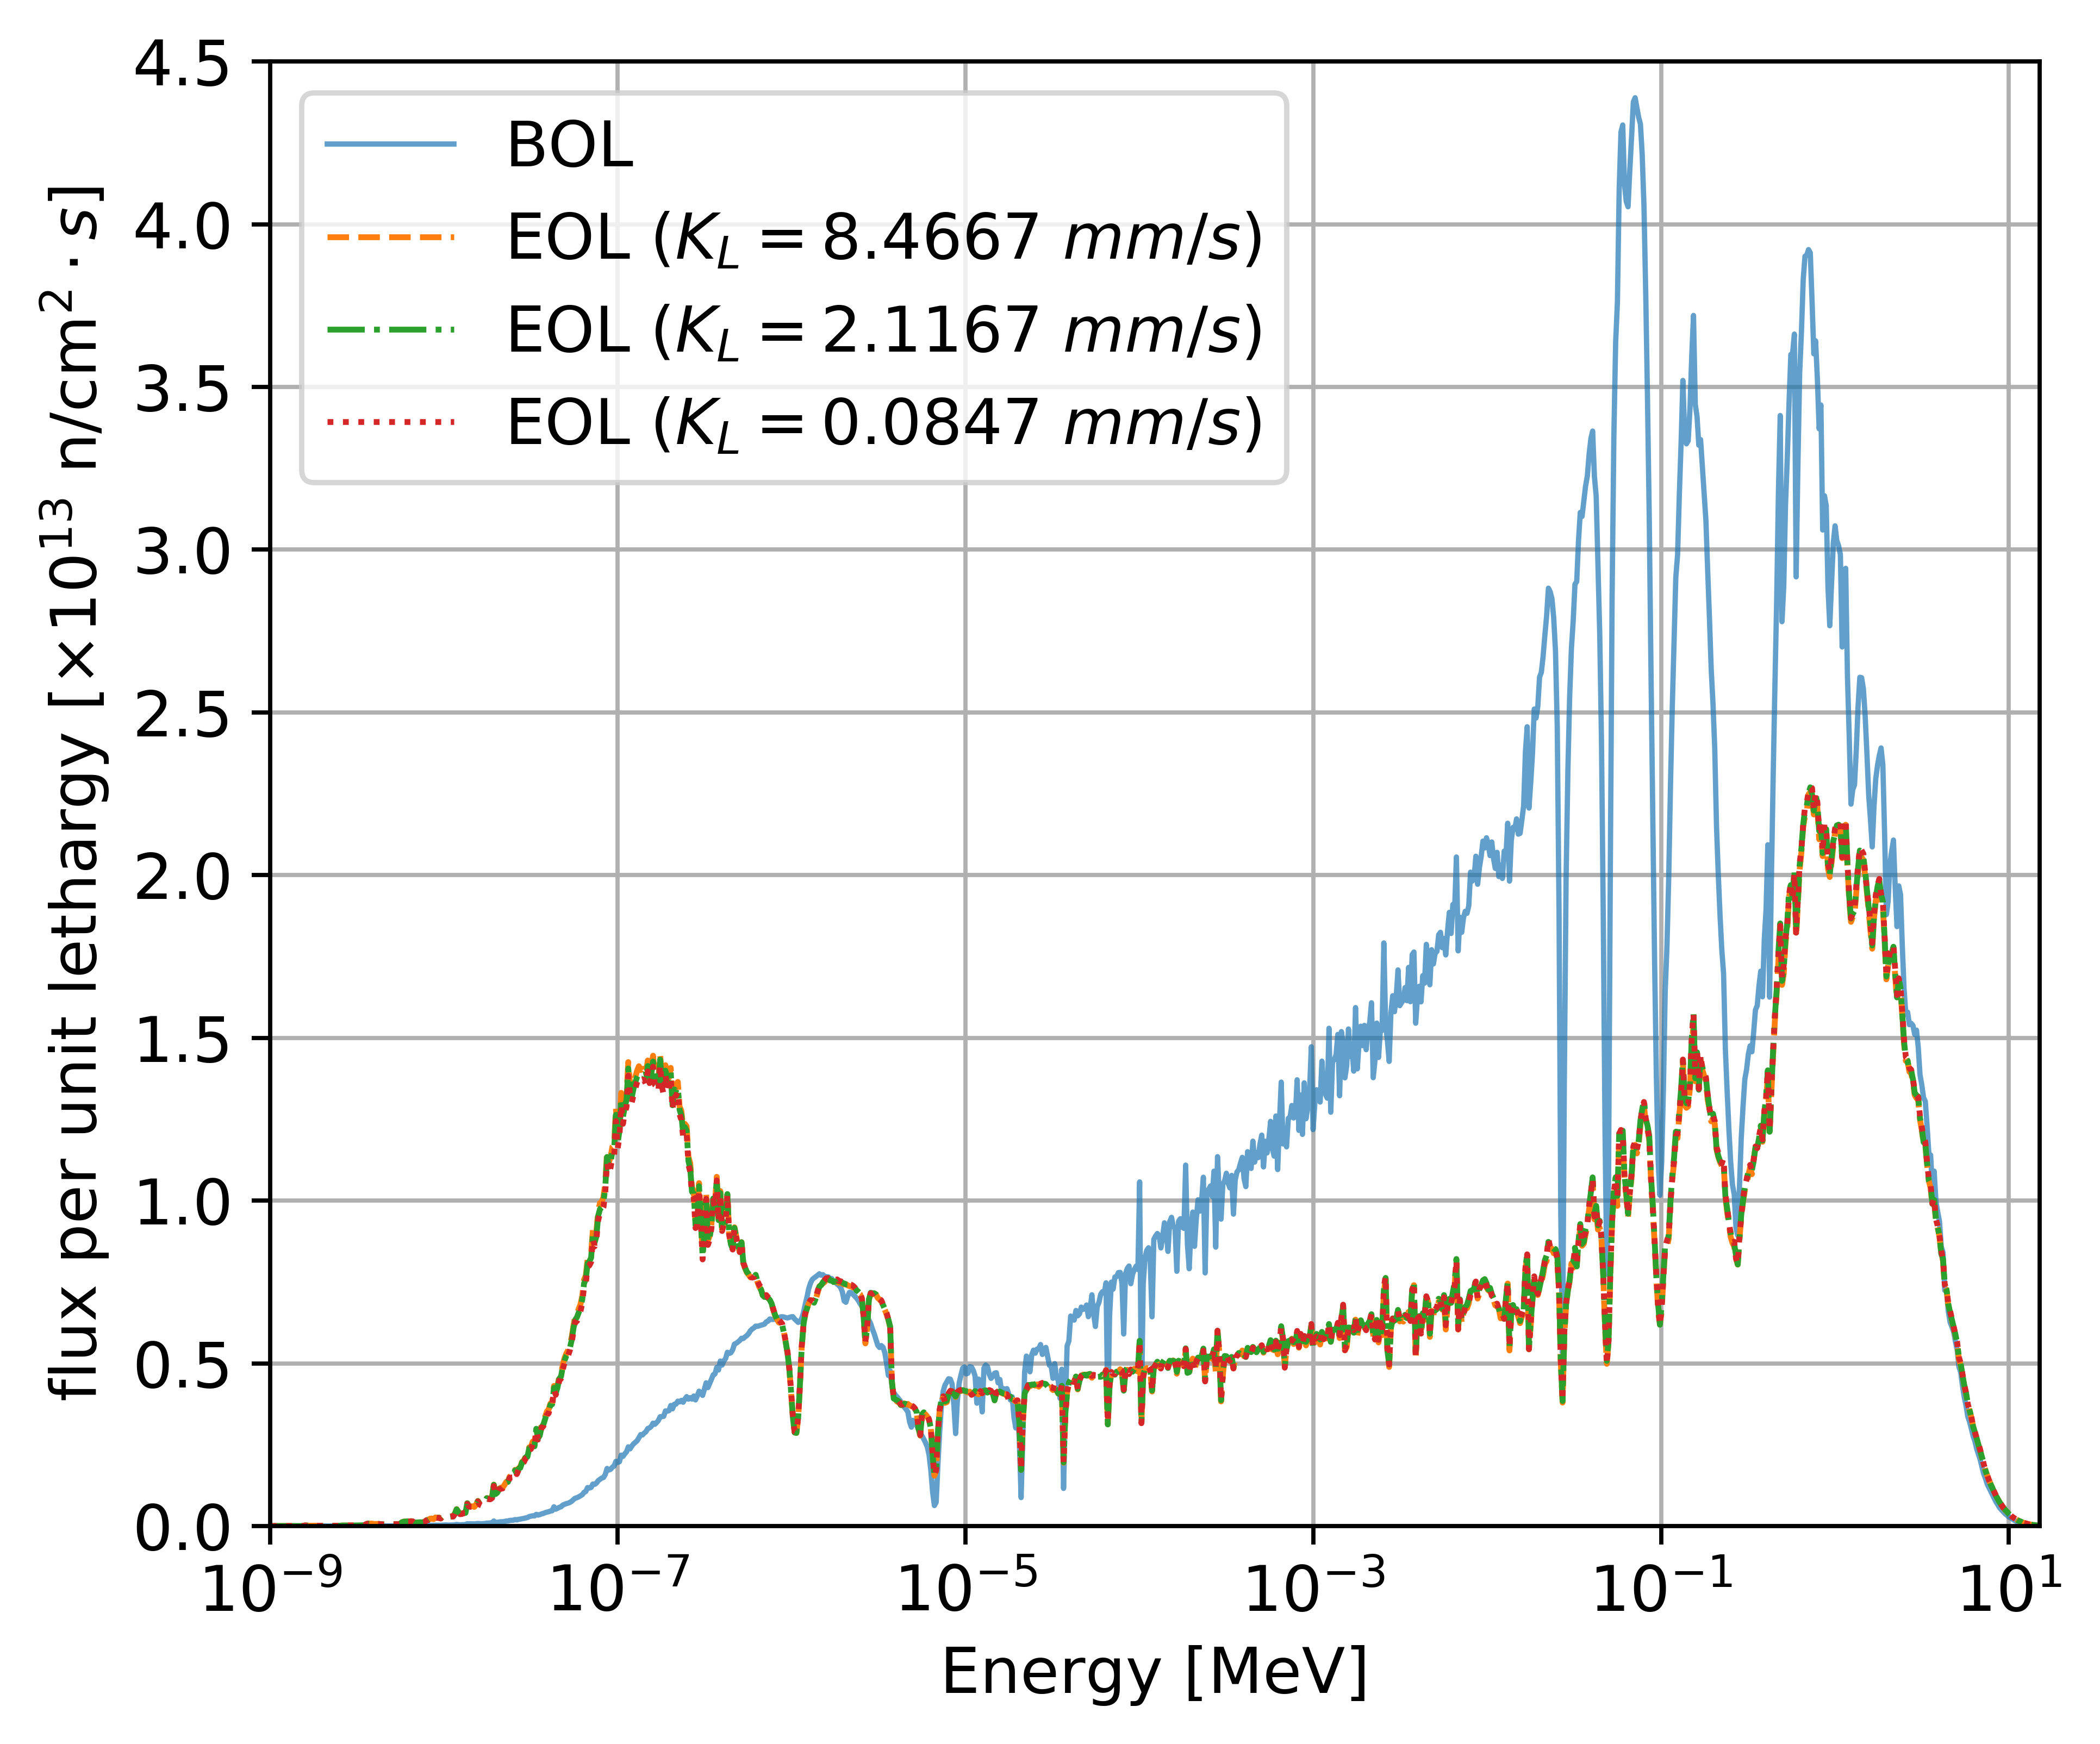
\includegraphics[width=0.65\textwidth]{../dissertation/figures/ch4/eps/spectrum.png}}
\onslide<2>\centerline{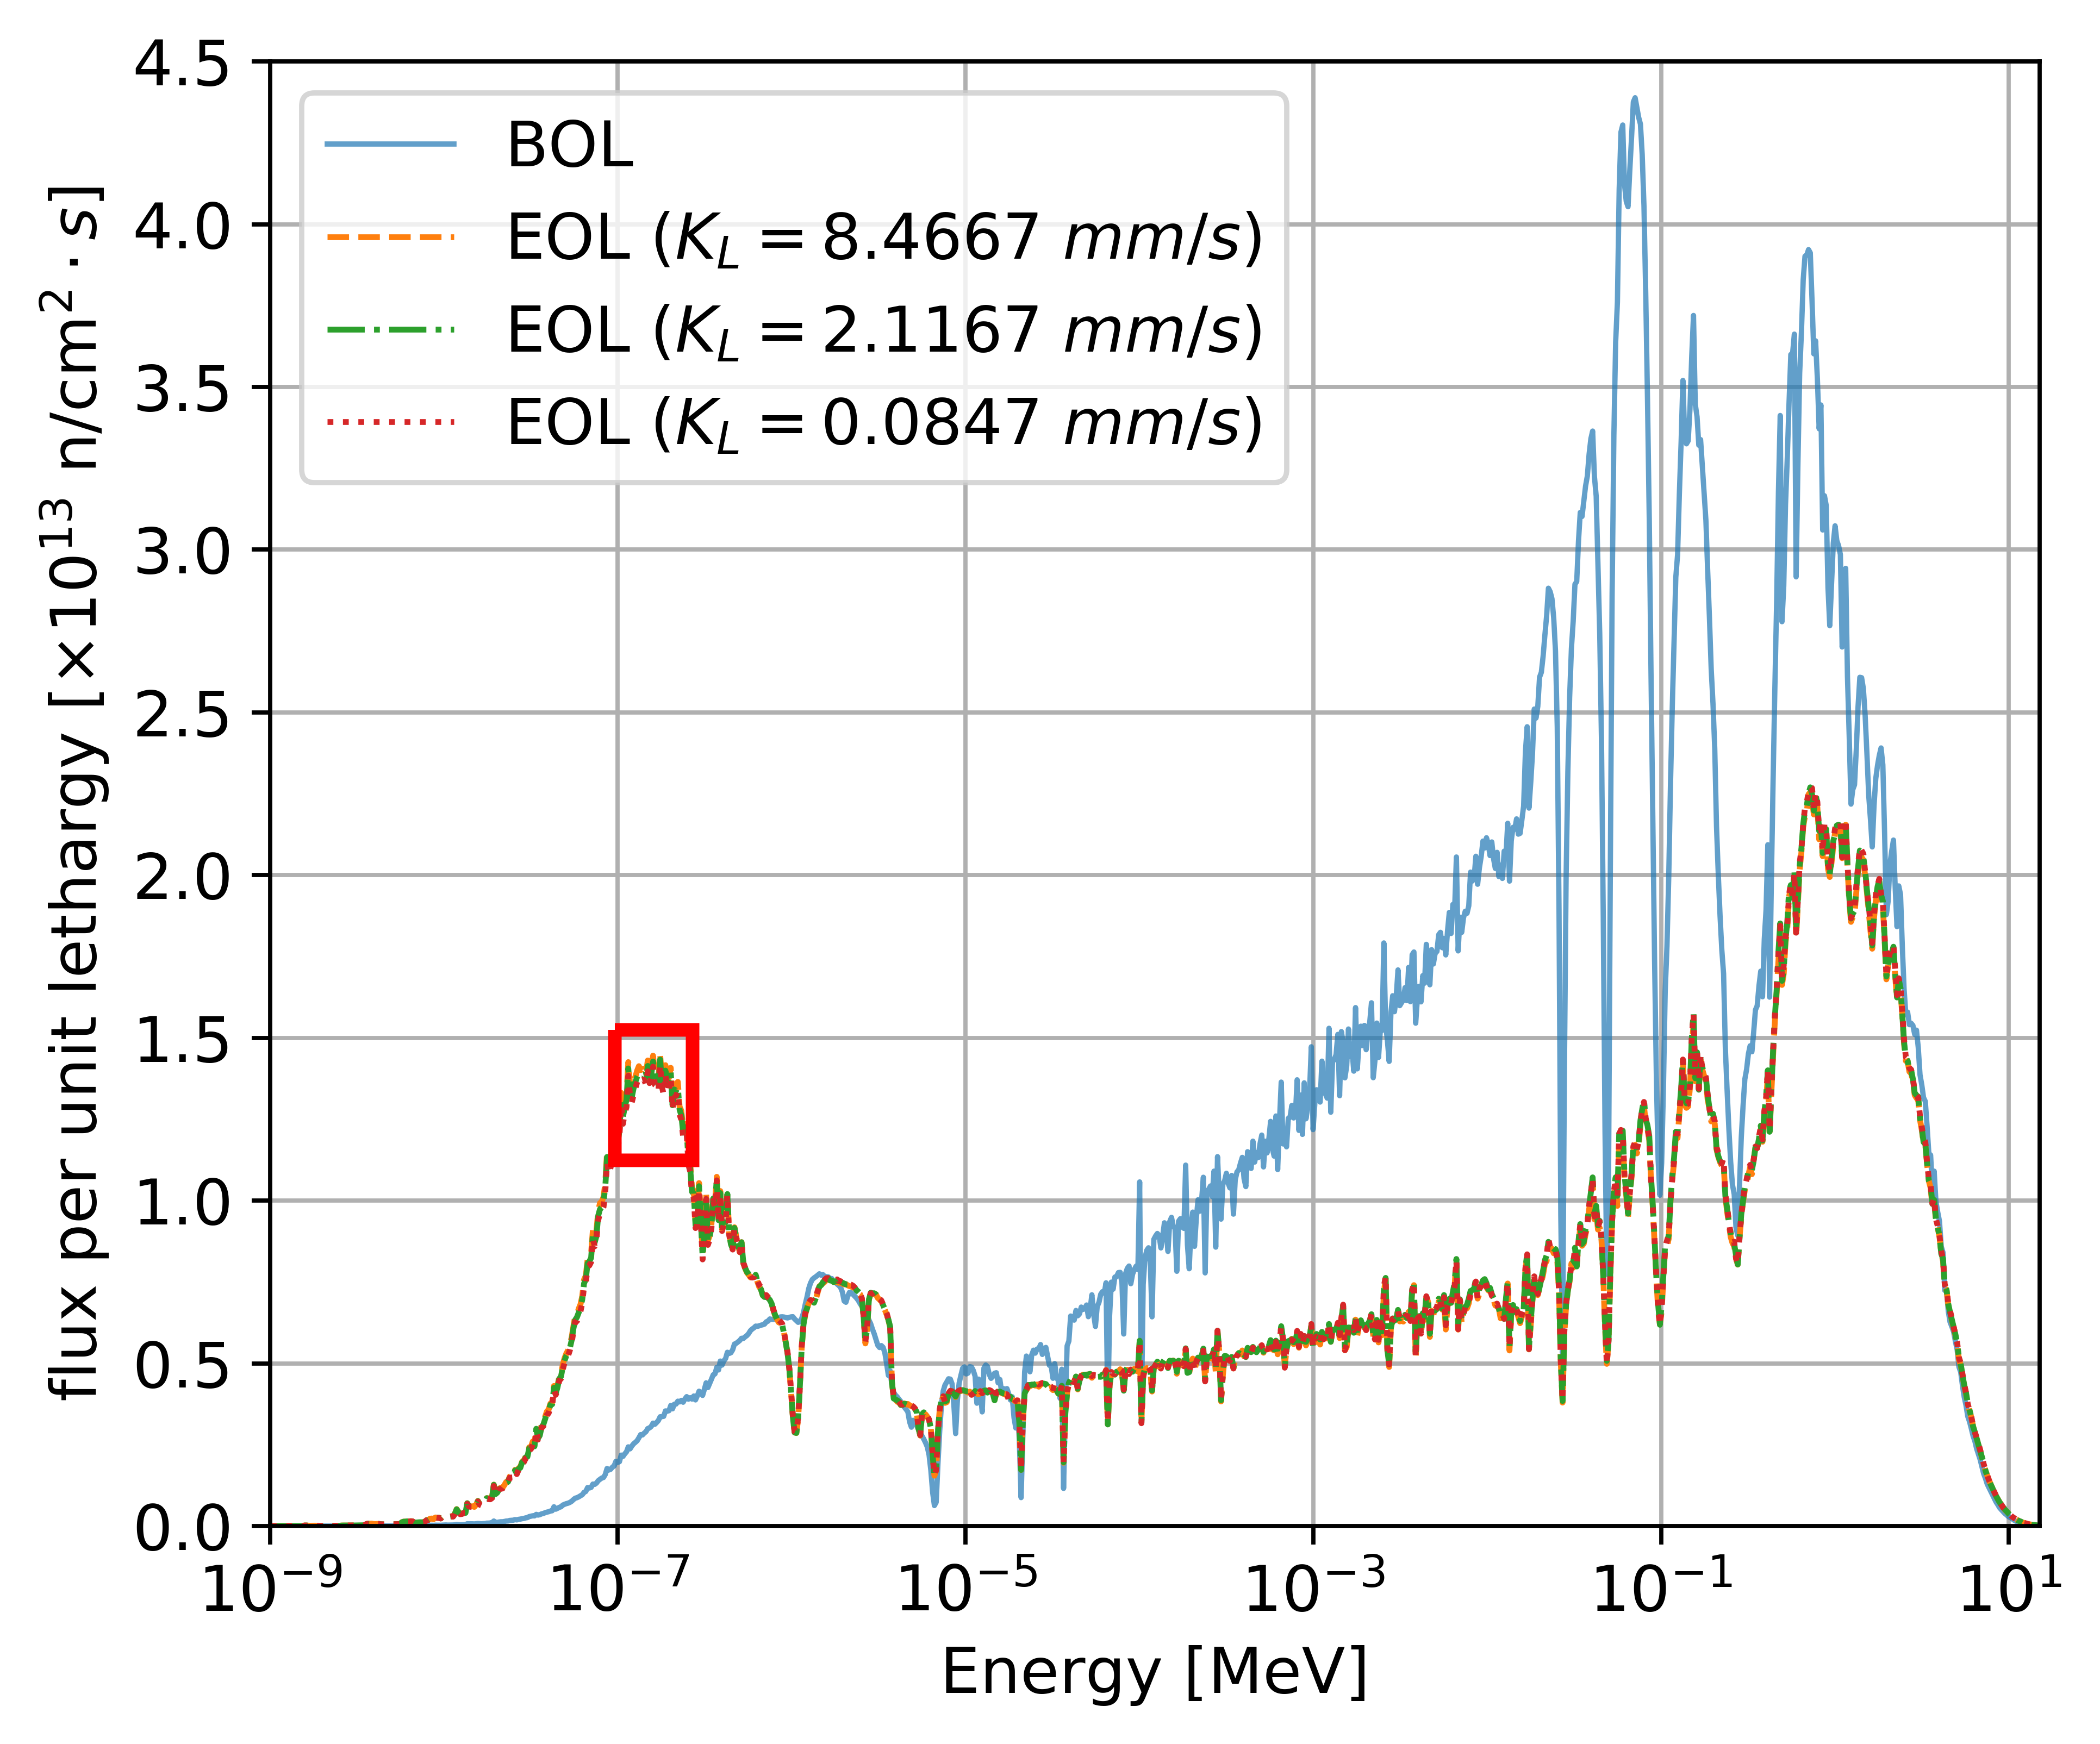
\includegraphics[width=0.65\textwidth]{./images/tap_sp_z_1.png}}
\onslide<3>\centerline{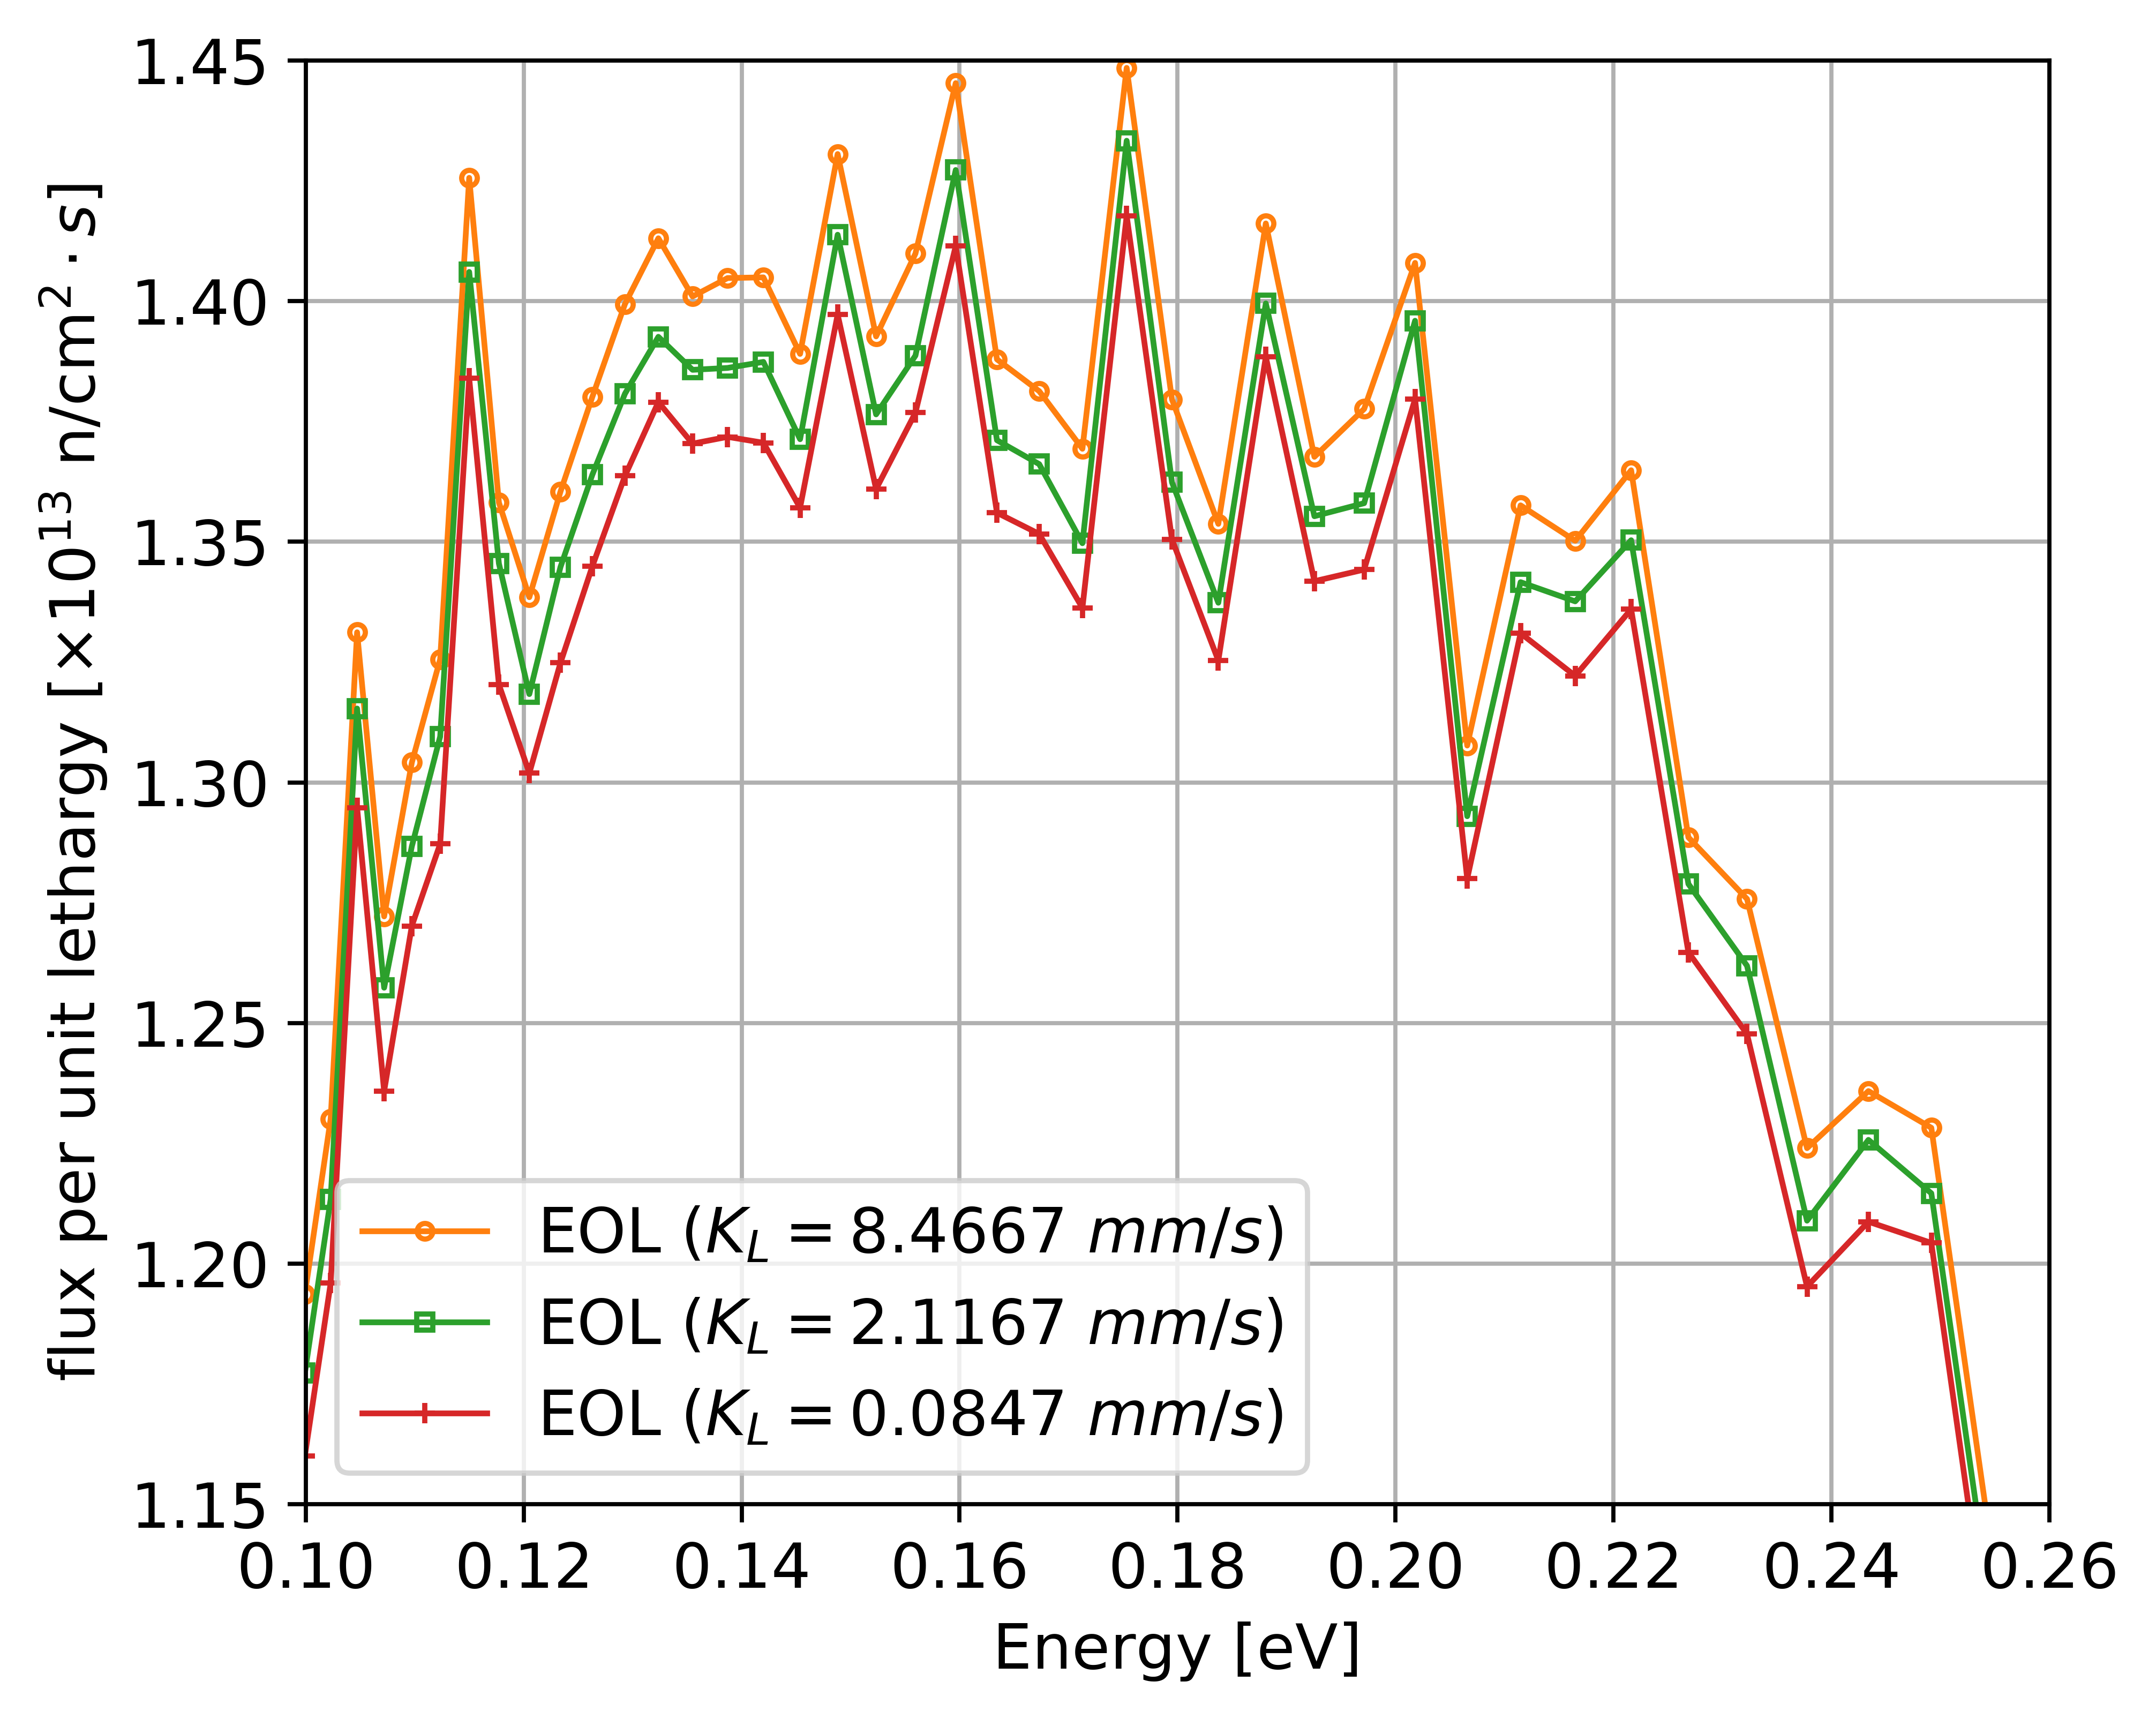
\includegraphics[width=0.67\textwidth]{../dissertation/figures/ch4/eps/spectrum_th_zoomed.png}}
		\end{overprint}
		\caption{The neutron flux energy spectrum normalized by unit lethargy 
		at the BOL and EOL. The neutron flux uncertainties $\sigma_{\Phi}$ are 
		0.6\% and 0.18\% for the \gls{TAP} reactor and \gls{MSBR}, 
		respectively.}
	\end{figure}
\end{textblock*}
\end{frame}


\begin{frame}
\frametitle{Fuel salt composition evolution during the TAP operation (1/2)}
\begin{textblock*}{12.25cm}(0.25cm,1.8cm) % {block width} (coords)
	\begin{figure}[htp!] % replace 't' with 'b' to 
		\centering
		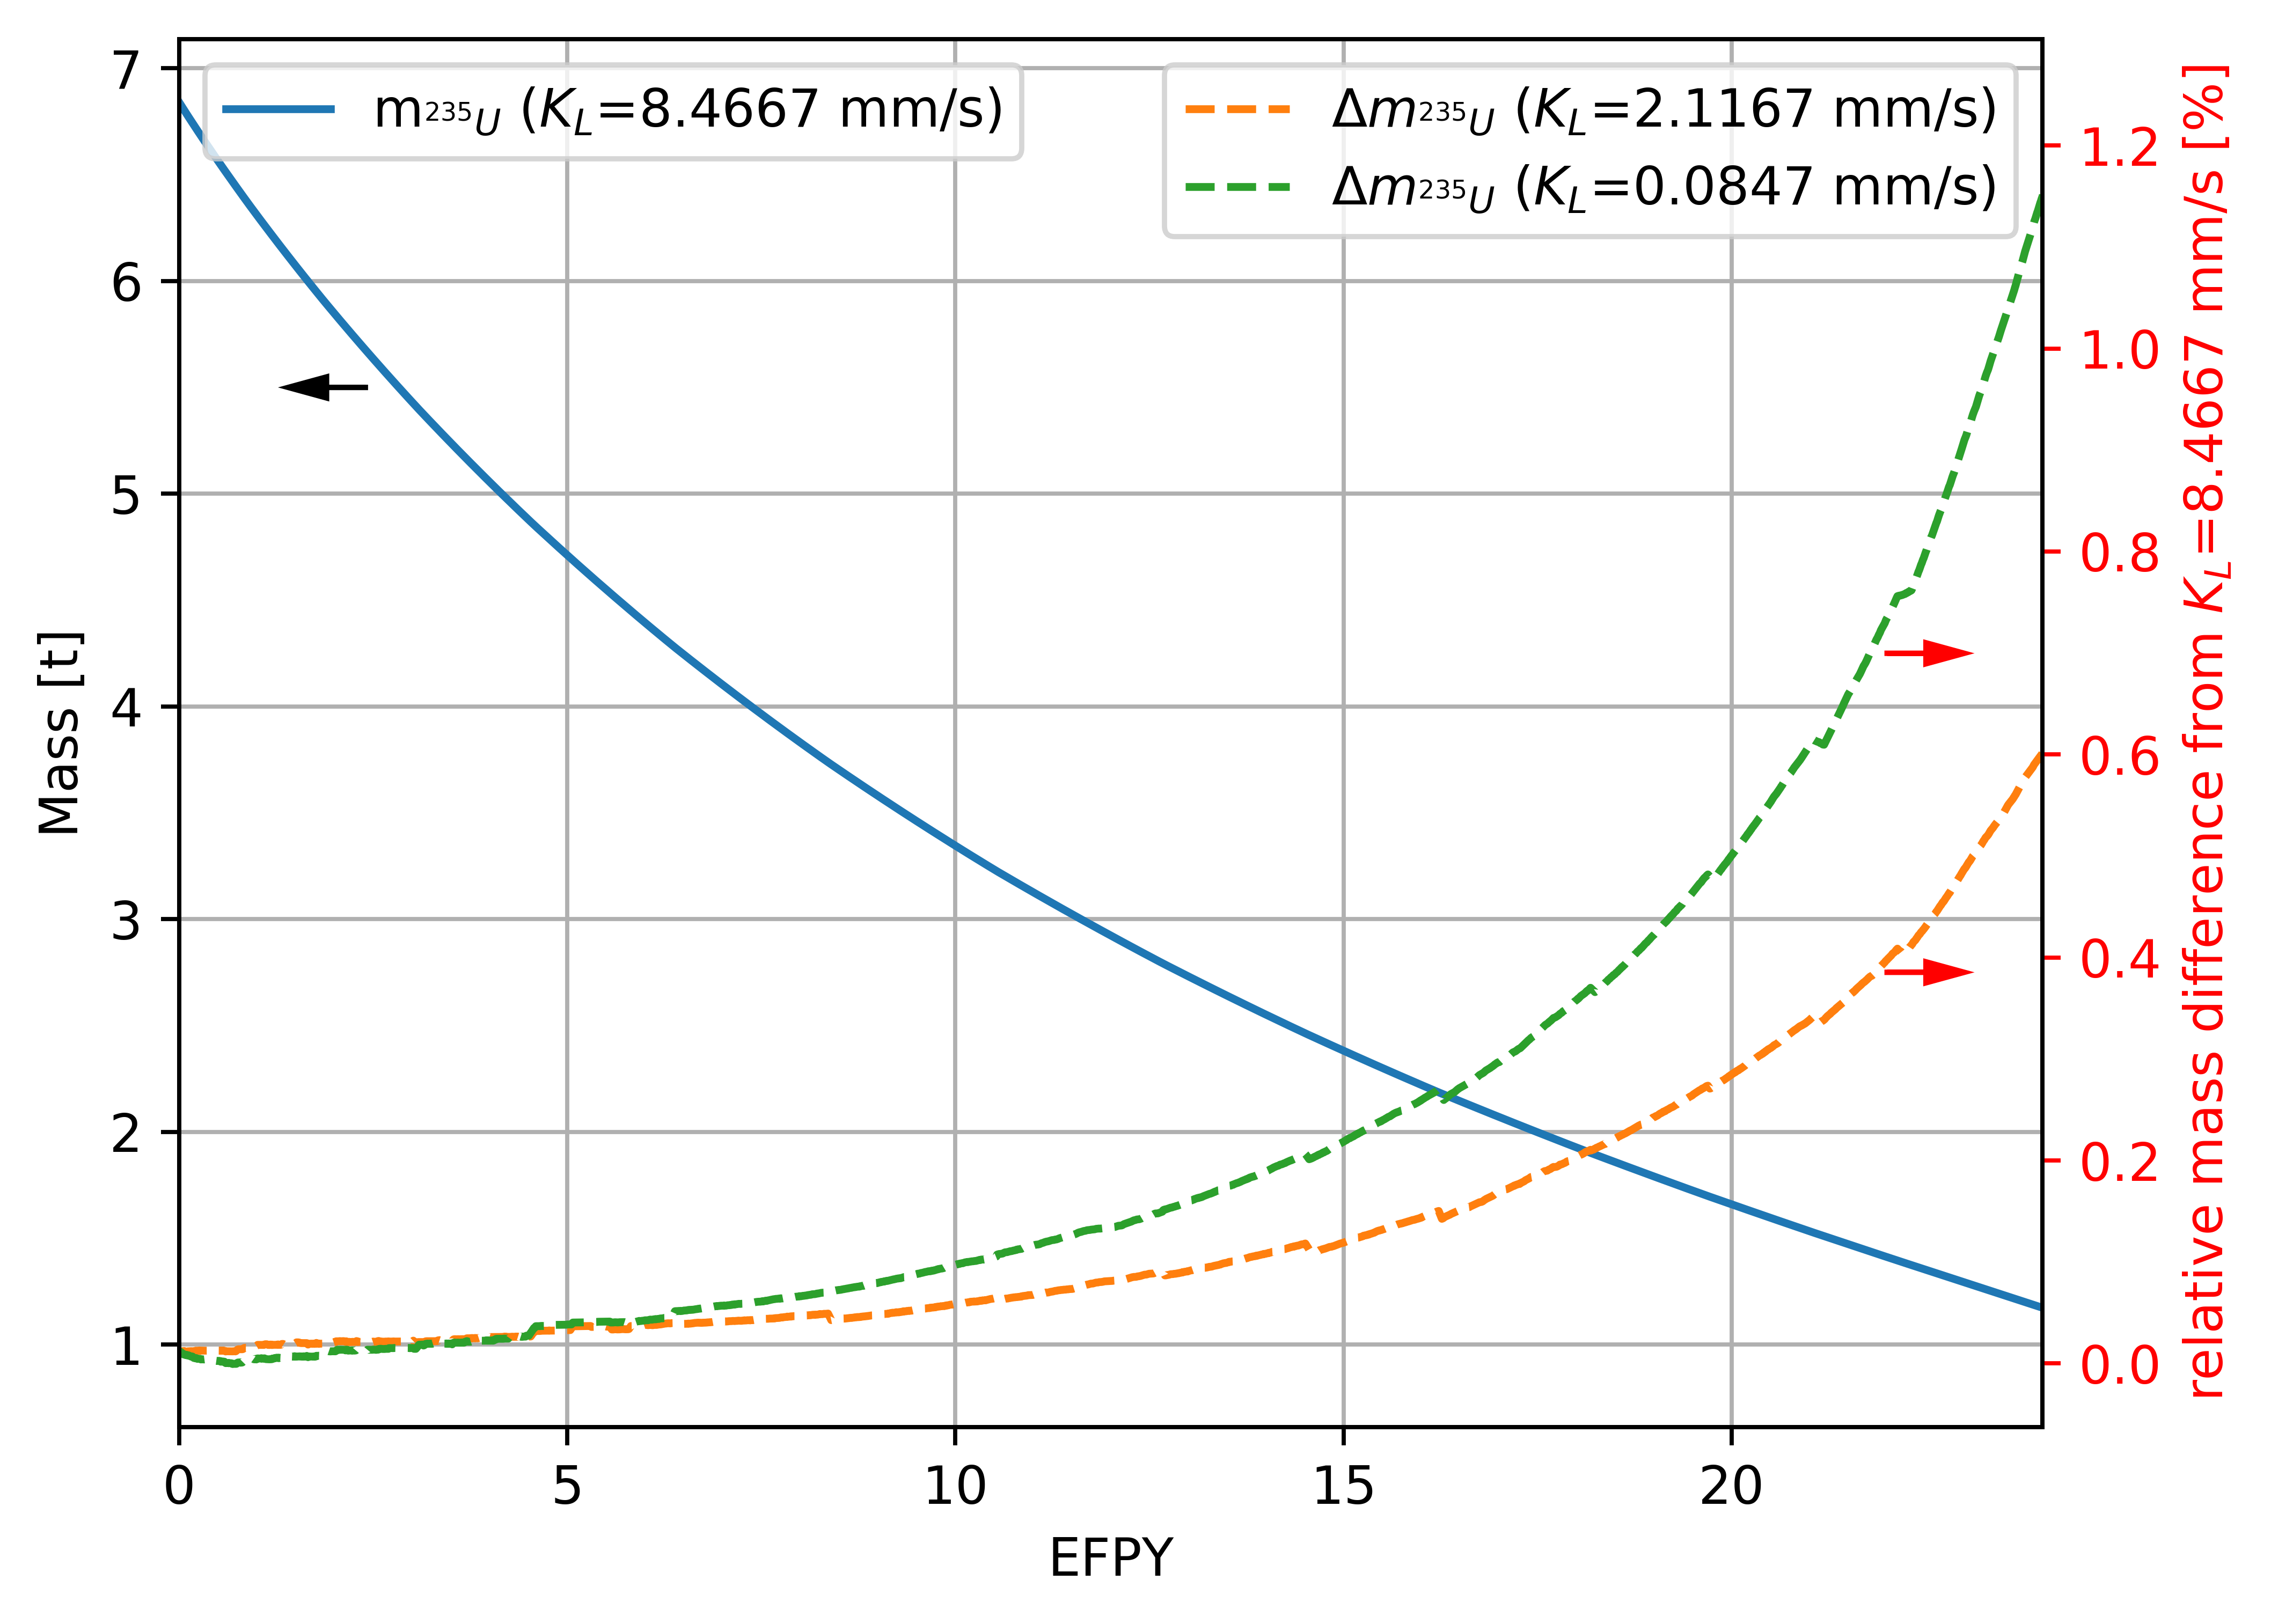
\includegraphics[width=0.75\textwidth]{../dissertation/figures/ch4/eps/u235.png}
			\vspace{-2mm}
		\caption{SaltProc-calculated mass of $^{235}$U in the fuel salt during 
		25 years of operation
for K$_L$ = 8.4667 mm/s compared with less 
		effective noble gas removal.}
	\end{figure}
\end{textblock*}
\end{frame}

\begin{frame}
\frametitle{Fuel salt composition evolution during the TAP operation (2/2)}
\begin{textblock*}{12.25cm}(0.25cm,1.8cm) % {block width} (coords)
	\begin{figure}[htp!] % replace 't' with 'b' to 
		\centering
		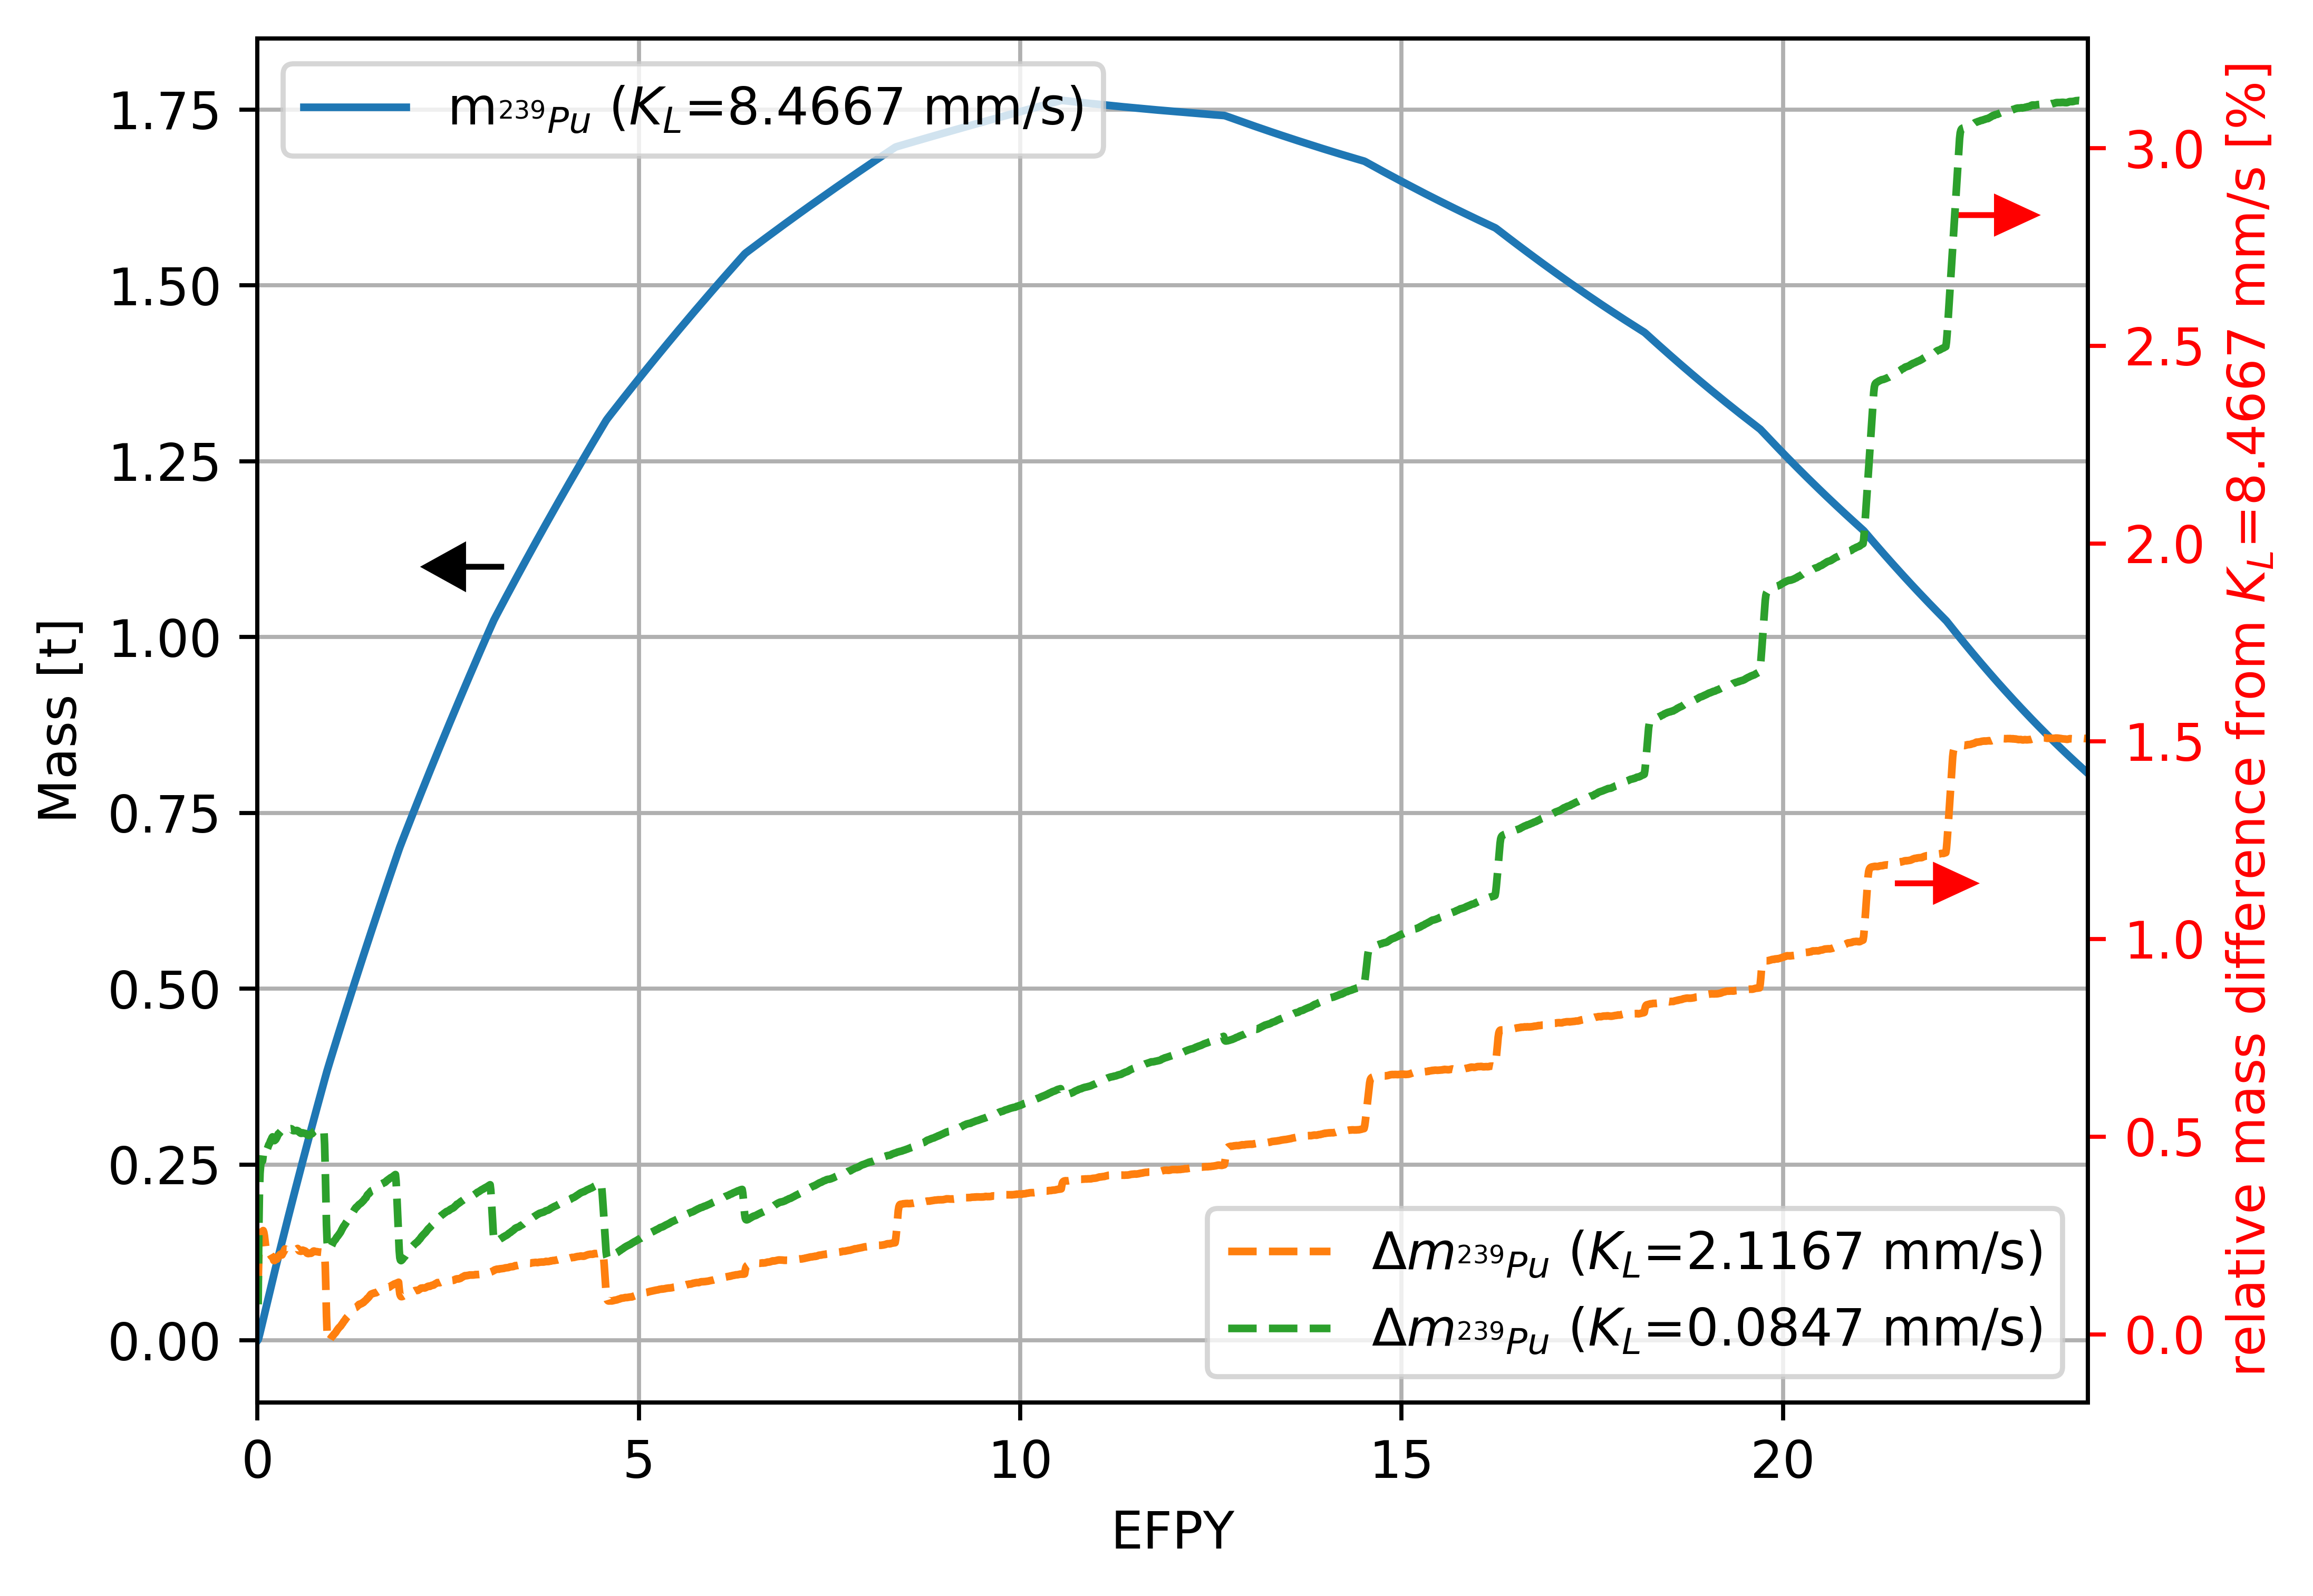
\includegraphics[width=0.77\textwidth]{../dissertation/figures/ch4/eps/pu239.png}
		\vspace{-1mm}
		\caption{SaltProc-calculated mass of $^{239}$Pu in the fuel salt 
		during 25 years of operation for K$_L$ = 8.4667 mm/s compared with 
		less effective noble gas removal.}
	\end{figure}
\end{textblock*}
\end{frame}


\begin{frame}
\frametitle{Impact of xenon poisoning on fuel cycle performance}
\begin{textblock*}{12.4cm}(0.07cm,2.1cm) % {block width} (coords)
	\begin{columns}
		\column[t]{5.5cm}
		\vspace{-5mm}
		\begin{figure}[hbp!] % replace 't' with 'b' to 
			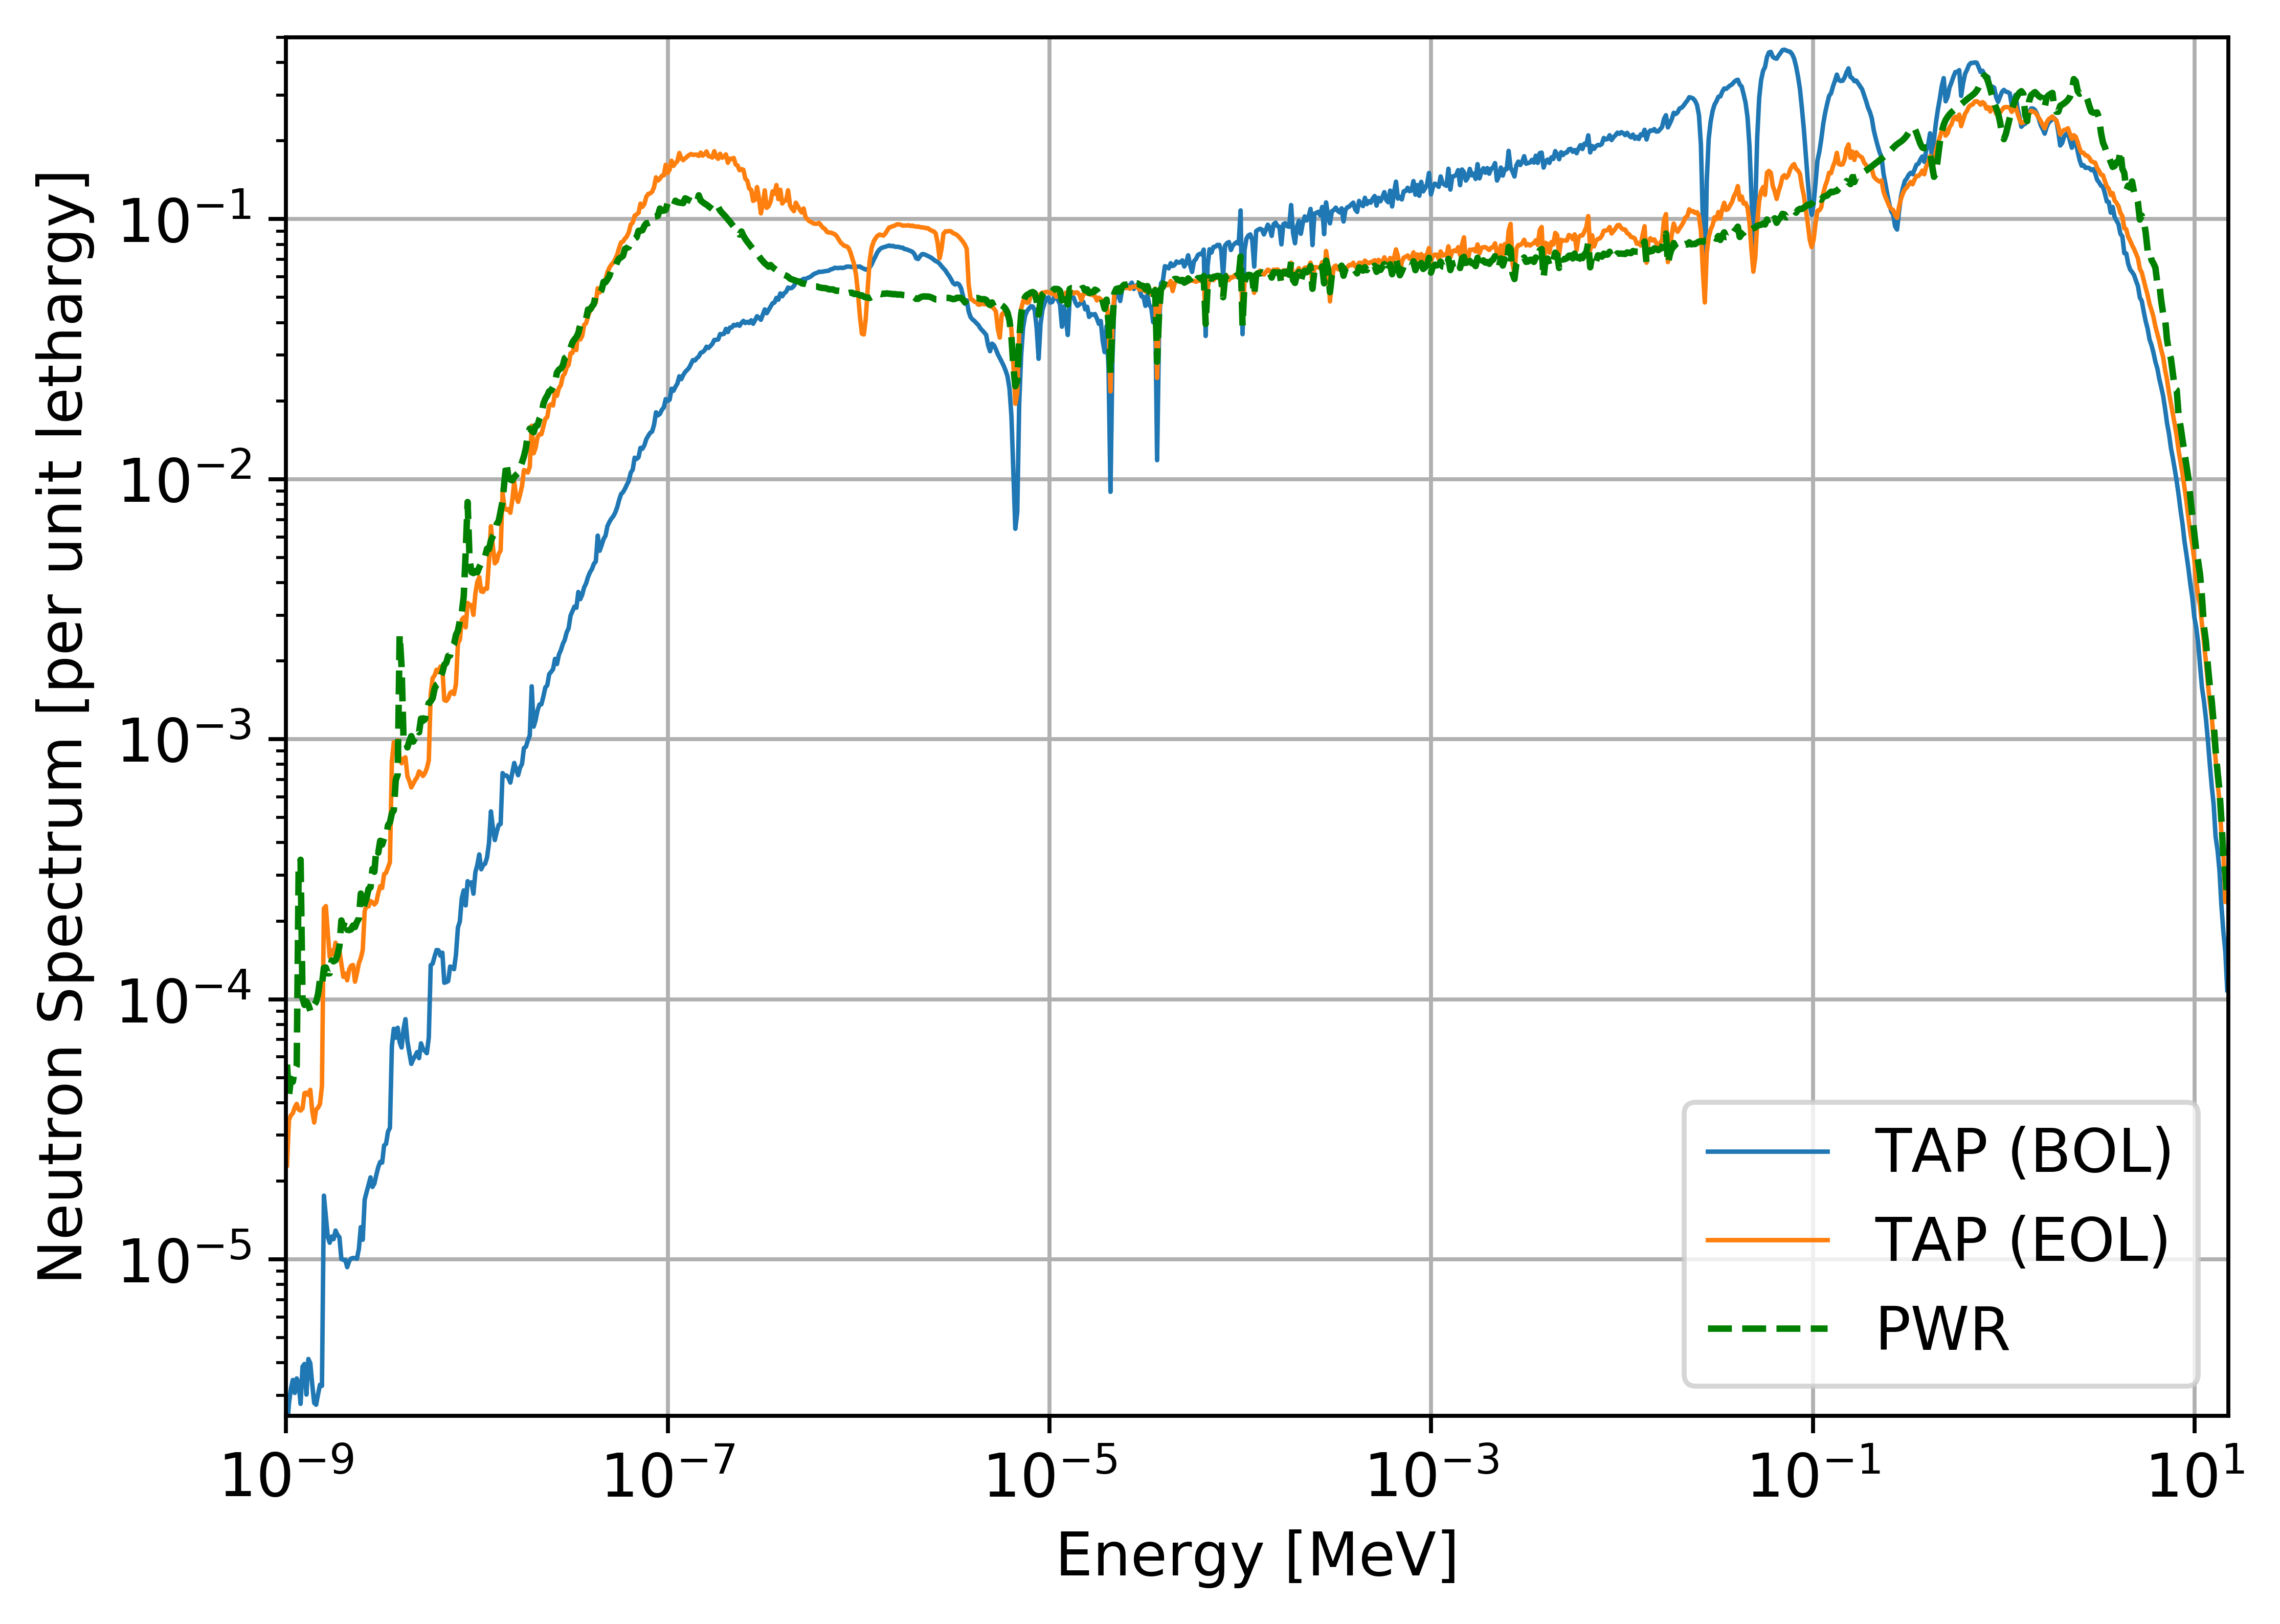
\includegraphics[width=0.94\textwidth]{../dissertation/figures/ch5/tap_vs_pwr_spectrum_2.png}\\
			\vspace{-5mm}
			\hspace{+0.05mm}
			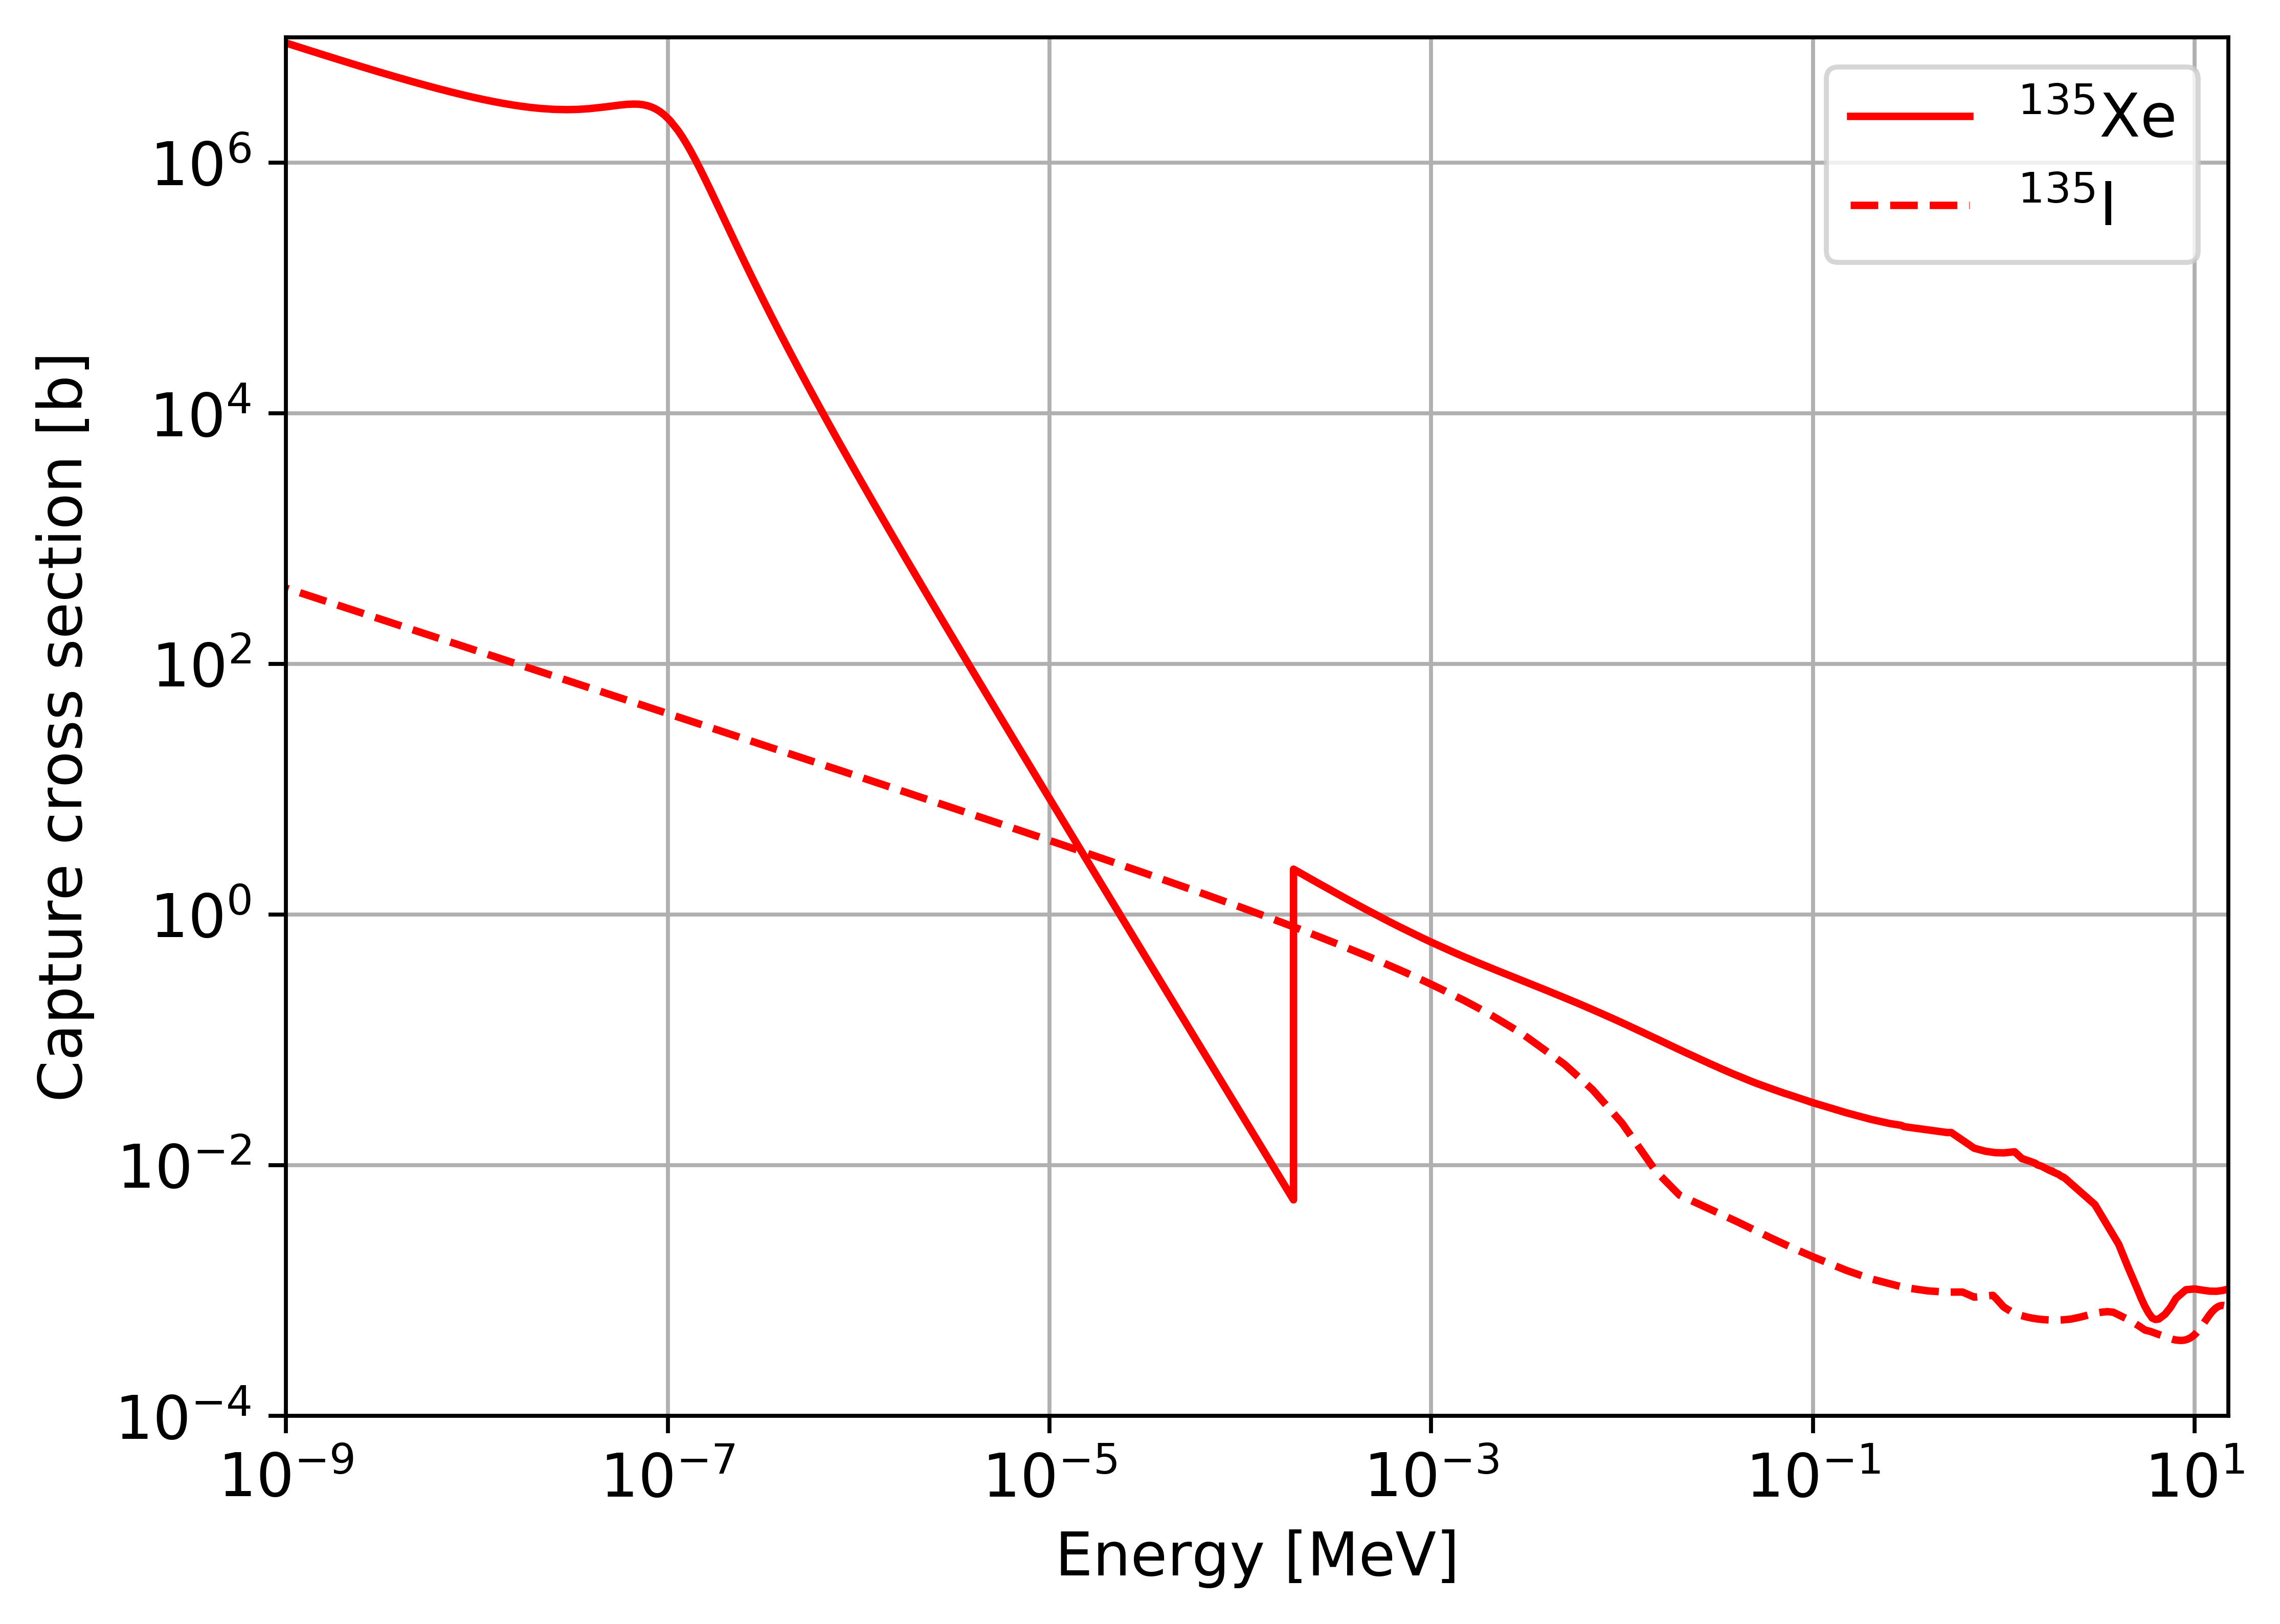
\includegraphics[width=0.94\textwidth]{../dissertation/figures/ch5/i_xe_xs.png}
			\vspace{-3mm}
			\caption{Neutron spectra (upper) and $^{135}$I, $^{135}$Xe caption 
			cross section (lower) \cite{rykhlevskii_impact_2019}.}
		\end{figure}
		
		\column[t]{6cm}
		\begin{textblock*}{7.3cm}(5.6cm,2.1cm) % {block width} (coords)
		\begin{itemize}
			\itemsep=0.3em
			\item \textbf{Less effective} gas removal leads to \textbf{harder} 
			spectrum
			\begin{itemize}
				\itemsep=0.5em
				\item Shorter lifetime due to parasitic absorption
				\item Lower $^{235}$U fission rate
				\item Faster rate of $^{238}$U destruction (-50kg)
				\item Increased breeding of fissile Pu
			\end{itemize}
			
			\item TAP spectrum \textbf{softens toward EOL}
			\begin{itemize}
				\itemsep=0.5em
				\item Reduced fissile Pu breeding after 11yrs
				\item $\alpha_T$ weakened 
				from $-1.57$ to $-0.26pcm/K$
				\item 12\% CRW degradation
				\item 39\% void coefficient of reactivity ($\alpha_V$) 
				degradation
				\item Lower reactor kinetic parameters ($\beta_{eff}$, 
				$\lambda_{eff}$)
			\end{itemize} 
		\end{itemize}
	
	{\par\small	These observations must be considered during the reactor 
	designing, accident analysis, and safety justification.}
		\end{textblock*}
	
	
	\end{columns}
\end{textblock*}
\end{frame}
\subsection{Short-term depletion: TAP MSR}


\begin{frame}
\frametitle{Why is load following a game changer?}
\begin{textblock*}{12.1cm}(0.3cm,1.65cm) % {block width} (coords)
	\begin{figure}[t]
		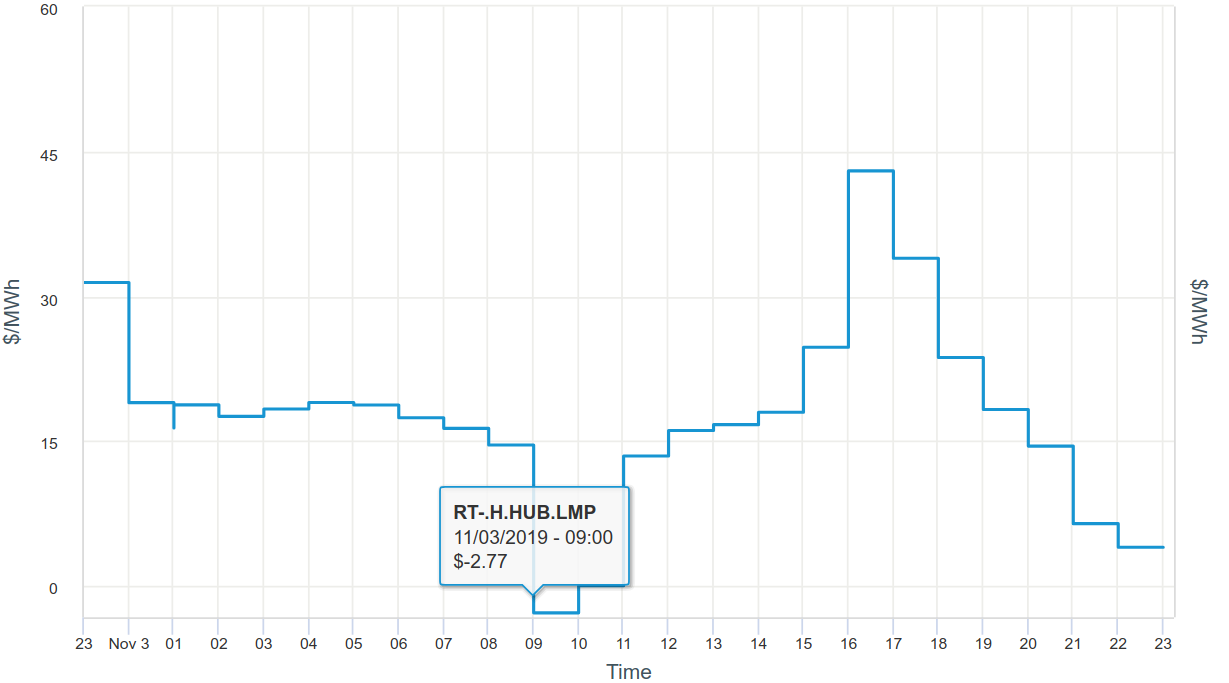
\includegraphics[width=0.65\textwidth]{./images/ne_one_day_price.png}
		\vspace{-2mm}
		\caption{ISO New England hourly electricity price; Nov 3, 2019 
			from 00:00AM to 11:00PM (Source: https://www.iso-ne.com/).}
	\end{figure}  
	\vspace{-4mm}
	
	\visible<2->{\begin{block}{Physical constraints limiting power 
	variations	in 
				Light-Water	Reactors \cite{lokhov_technical_2011}:}
			\begin{itemize}
				\item thermal strain and stress to fuel materials
				\item fuel burnup (insufficient excess reactivity at the 
				EOC)}
			\item<3-> \textbf{$^{135}Xe$ poisoning (iodine pit)}
		\end{itemize}
	\end{block}
\end{textblock*}
\end{frame}


\begin{frame}
\frametitle{What is $^{135}$Xe poisoning? \cite{nuclear_power_production_2020}}
\animategraphics[loop,controls,width=1.07\linewidth]{0.5}{./images/anime/xe_pois-}{0}{11}
\end{frame}


\begin{frame}
\frametitle{Postulated worst-case load-following scenario}
\vspace{-6mm}
\begin{columns}
	\column[t]{5.5cm}
	\begin{figure}[t]
		\includegraphics[width=\linewidth]{./images/power_load_curve.png}
		\vspace{-6mm}
		\caption{Postulated load-following power transient.}
	\end{figure}
	
	\column[t]{6.3cm}
	\begin{block}{Postulated load-following transient}
		\begin{enumerate}             
			\item $P(t<t_{eq})=100$\% to reach $^{135}$Xe/$^{135}$I equilibrium
			\item instantaneous power drop from 100 to 0\%
			\item $P(t_{eq}<t<t^{max}_{X})=0$\% to reach the 
			$^{135}$Xe peak
			\item restart instantly from 0 to 100\%, and then operation on 
			100\% for a few hours
		\end{enumerate}
			\vspace{-3mm}
	\end{block}
		{\footnotesize
		\begin{align}\label{eq:time-xe-max}
		t^{max}_{X} &= t_{eq} + \frac{1}{\lambda_X-\lambda_I}
		log\left(\frac{\lambda_X(\lambda_I[X_0+I_0]-\lambda_XX_0)}{\lambda_I^2 
		I_0}\right) \nonumber
		\end{align}}
				\vspace{-3mm}
	\begin{block}{Simplifying assumptions}
		\begin{itemize}
			\item All control rods are fully withdrawn
			\item Fission power adjusted by changing normalization in Serpent 
			2 ($\overline{\phi}=0$)
			\item 15-min depletion step
		\end{itemize}
		
	\end{block}
\end{columns}
\end{frame}

\begin{frame}
\frametitle{TAP load-following simulation without gas removal}
\begin{textblock*}{12.5cm}(0.1cm,2.1cm) % {block width} (coords)
\begin{columns}
	\column[t]{6.3cm}
	\begin{figure}[t]
		\begin{overprint}
	\onslide<2>\includegraphics[width=1.11\linewidth]{../dissertation/figures/ch5/keff_kl_1_eol_eoc_15min.png}
		\vspace{-6mm}
	\caption{$k_{eff}$ dynamics during 2.75-hour shutdown (\textbf{10 days 
		before EOL}, \textbf{no gas removal}). $\sigma\pm7$ $pcm$ is shaded.}
	\onslide<3-4>\includegraphics[width=1.11\linewidth]{../dissertation/figures/ch5/xe_i_kl_1_eol_eoc_15min.png}
		\vspace{-6mm}
	\caption{Number density of $^{135}$Xe and $^{135}$I during anticipated 
	transient (\textbf{10 days before EOL}, \textbf{no gas removal}).}
		\end{overprint}
	\end{figure}
	
	\column[t]{5.5cm}
	\begin{textblock*}{6cm}(6.65cm,2.1cm) % {block width} (coords)
		\fontsize{7}{9}\selectfont
		\begin{itemize}
		\item<1-> Negligible xenon poisoning at BOL
	\setbeamerfont*{itemize/enumerate body}{size=\footnotesize}
	\setbeamerfont*{itemize/enumerate subbody}{parent=itemize/enumerate 
	body}
	\setbeamerfont*{itemize/enumerate subsubbody}{parent=itemize/enumerate 
	body}			
			\begin{itemize}
				\item $\rho_X\approx-10\pm7$ $pcm$
				\item $^{135}$Xe concentration change $+0.33$\%
				\item $N_{^{135}I}/N_{^{135}Xe}<0.8$ due to hard spectrum
			\end{itemize} 
			\item<2-> Weak xenon poisoning at EOL (10d before shutdown, all 
			moderator rods are inserted)
	\setbeamerfont*{itemize/enumerate body}{size=\footnotesize}
	\setbeamerfont*{itemize/enumerate subbody}{parent=itemize/enumerate 
		body}
	\setbeamerfont*{itemize/enumerate subsubbody}{parent=itemize/enumerate 
		body}			
			\begin{itemize}
				\item $\rho_X\approx-70\pm7$ $pcm$
				\item<3-> $^{135}$Xe concentration change $+4$\%
				\item<3-> $N_{^{135}I}/N_{^{135}Xe}\approx1.0$
			\end{itemize}
		\end{itemize}
				\vspace{+5mm}
		\begin{block}<4->{\qquad Main takeaways}
			\begin{itemize}
				\item TAP \textbf{can load-follow} throughout whole
			lifetime \textbf{without significant $^{135}$Xe poisoning}
				\item Noble gas removal \textbf{unnecessary for load-following 
				in TAP}
				\item Noble gas removal \textbf{beneficial for long-term 
				performance}
				\item Main reason - \textbf{relatively fast neutron spectrum} 
				of TAP MSR
			\end{itemize}
		
	\end{block}
	\end{textblock*}
\end{columns}
\end{textblock*}
\end{frame}



\begin{frame}
\frametitle{Safety parameters evolution during load-following (EOL)}
\begin{textblock*}{12.5cm}(0.1cm,2.1cm) % {block width} (coords)
	\begin{columns}
		\column[t]{6.3cm}
		\begin{figure}[t]
			\begin{overprint}
	\onslide<1>\includegraphics[width=1.15\linewidth]{../dissertation/figures/ch5/saf_par/tc_evo.png}
	\vspace{-6mm}
	\caption{Temperature feedback coefficients as a function of time during 
	the transient. 
	Uncertainty $\pm\sigma$ is shaded.}
	\onslide<2>\includegraphics[width=1.15\linewidth]{../dissertation/figures/ch5/saf_par/void_evo.png}
	\vspace{-6mm}
	\caption{Void coefficient of reactivity ($\alpha_V$) as a function of time 
	during the transient.}
	\onslide<3->\includegraphics[width=1.15\linewidth]{../dissertation/figures/ch5/saf_par/crw_evo.png}
	\vspace{-6mm}
	\caption{Total control rod worth as a function of time during the 
	transient.}
			\end{overprint}
		\end{figure}
		
		\column[t]{5.5cm}
		\begin{textblock*}{5.9cm}(6.9cm,2.6cm) % {block width} (coords)
			\begin{itemize}
				\itemsep=0.8em
				\item<1-> Fuel temperature coefficient ($\alpha_{T,F}$) 
				worsened during first 3 hours when $^{135}$Xe concentration 
				peaked causing the spectrum hardening
				\item<2-> $\alpha_V$ fluctuates in stochastic uncertainty 
				range $\sigma_{\alpha_V}\pm4$ $pcm/$\%
				\item<3-> CRW worsened right after shutdown but then quickly 
				recovered due to quick $^{135}$Xe removal
				\item<4-> TAP reactor maintains safety margins during the 
				load-following transient
			\end{itemize}
				
		\end{textblock*}
	\end{columns}
\end{textblock*}
\end{frame}


\subsection{Short-term depletion: MSBR}

\begin{frame}
\frametitle{Xenon poisoning effect during MSBR load-following}
\vspace{-8mm}
\begin{columns}
	\column[t]{7cm}
	\visible<2->{
	\begin{figure}[t]
	\centering
$\begin{array}{r}
\includegraphics[width=0.717\textwidth]{../dissertation/figures/ch6/kl1_rho.png}\vspace{-5mm}\\
\includegraphics[width=0.70\textwidth]{../dissertation/figures/ch6/kl25_rho.png}\vspace{-5mm}\\
\includegraphics[width=0.70\textwidth]{../dissertation/figures/ch6/kl100_rho.png}
\end{array}$
\vspace{-4mm}
\caption{$\rho(t)$ during the transient ($\pm\sigma_{\rho}=10$$pcm$).}
	\end{figure}}
	
	\column[t]{5.5cm}
	\begin{textblock*}{6.1cm}(6.3cm,2cm) % {block width} (coords)
	\begin{block}<1->{Analysis assumptions}
				\fontsize{7}{9}\selectfont
		\begin{enumerate}             
			\item Load profile similar to TAP reactor
			\item $t^{max}_X\approx7.5h$
			\item 30-min depletion step
			\item Low, medium, and high gas removal efficiency
		\end{enumerate}
		\vspace{-1mm}
	\end{block}

	\begin{block}<2->{Key takeaways}
				\fontsize{7}{9}\selectfont
		\begin{itemize}
			\item MSBR \textbf{cannot load-follow without gas removal:} 
			$\Delta\rho=-1490pcm$
			\item Xenon poisoning is \textbf{milder toward EOL} due to 
			spectrum \textbf{hardening}
			\item Huge \textbf{positive reactivity insertion} for medium 
			and high removal efficiency
			\item Even removal of \textbf{53.6\%} of Xe significantly 
			reduced the effect of poisoning: \textbf{-161$\pm10pcm$}
			\item More effective removal (\textbf{91.5\%}) gave similar 
			improvement: \textbf{-189$\pm10pcm$}
		\end{itemize}
		
	\end{block}
\end{textblock*}
\end{columns}
\end{frame}

\begin{frame}
\frametitle{Safety parameter evolution during load-following}
\begin{textblock*}{12.5cm}(0.4cm,1.55cm) % {block width} (coords)
	\begin{columns}
		\column[t]{6.3cm}
		\begin{figure}[t]
			\begin{overprint}
				\onslide<1>\includegraphics[width=0.87\linewidth]{./images/msbr_tc_evo.png}
				\vspace{-2mm}
				\caption{Temperature coefficients dynamics during the 
				transient.}
				\onslide<2>\includegraphics[width=0.87\linewidth]{./images/msbr_void_evo.png}
				\vspace{-1mm}
				\caption{Void coefficient of reactivity ($\alpha_V$) dynamics
					during the transient.}
				\onslide<3->\includegraphics[width=0.87\linewidth]{./images/msbr_crw_evo.png}
				\vspace{-1mm}
				\caption{Total control rod worth dynamics during 
				the transient.}
			\end{overprint}
		\end{figure}
		
		\column[t]{6cm}
		\begin{textblock*}{6.7cm}(6cm,2.6cm) % {block width} (coords)
			\begin{itemize}
				\itemsep=0.8em
				\item<1-> $\alpha_{T,ISO}$ worsens slightly as $^{135}$Xe 
				concentration spikes and then improves quickly
				\item<2-> $\alpha_V$ demonstrates similar behavior
				\item<3-> CRW worsens after shutdown but then quickly 
				improves due to quick $^{135}$Xe removal
				\item<4-> Total control rod worth is insufficient to shut down 
				the reactor at any time during transient
			\end{itemize}
			
		\end{textblock*}
	\end{columns}
\end{textblock*}
\end{frame}


\begin{frame}
\frametitle{Neutron energy spectrum MSBR vs TAP}
\begin{textblock*}{12.6cm}(0.1cm,1.6cm) % {block width} (coords)
	\begin{figure}[htp!] % replace 't' with 'b' to 
		\centerline{\includegraphics[width=0.73\textwidth]{../dissertation/figures/ch6/msbr_vs_tap_spectrum.png}}
		\vspace{-3mm}
		\caption{The neutron flux energy spectrum normalized by unit lethargy 
		for 
			MSBR and TAP at BOL and EOL. }
	\end{figure}
\end{textblock*}
\end{frame}
\section{Conclusions}
\chapter{Conclusions and future work}

\section{General Conclusions}
Liquid-fueled nuclear reactors offer several advantages over their traditional 
solid-fueled counterparts, which makes them a promising option for nuclear 
fuel cycle closure while offering improved inherent safety. Simulating such 
systems presents a challenge because existing reactor physics software for 
fuel burnup historically has been developed for traditional, solid-fueled 
reactors.

This work demonstrated a flexible, open-source tool, SaltProc, for 
simulating fuel depletion in a wide range of circulating-fuel (e.g., liquid 
fuel circulating throughout the primary loop) nuclear reactors that takes into 
account unique features of such systems: online fuel reprocessing 
and refueling. SaltProc extends the continuous-energy Monte Carlo burnup 
calculation code, Serpent 2, for the simulation of material isotopic evolution 
in any nuclear reactors with circulating, liquid fuel with the main focus on 
the liquid-fueled \glspl{MSR}. This work demonstrates a clear contribution to 
the nuclear engineering community by providing a tool for fuel depletion 
calculations in any generic nuclear system with circulating fuel.

The need for this work has been shown by a summary of the current state of the 
art of \gls{MSR} depletion simulator capabilities. The literature review in 
Chapter 1 concluded that most \gls{MSR} depletion simulators typically assume 
ideal (rather than realistically constrained) poison removal rates for the 
nuclear system performance modeling. Moreover, most of the simulators assumed 
constant extraction efficiency vectors, which must be determined by the user 
in the input file and cannot be a function of other parameters. SaltProc is 
capable of modeling the peculiarities of \glspl{MSR}, namely:
complex, multi-component reprocessing system structure and realistic 
extraction efficiency of fission product described as a function of 
many parameters. Furthermore, SaltProc can maintain reactor criticality by 
adjusting the reactor core geometry. In addition to fundamental simulation 
capabilities, SaltProc has a scalable design and allows the development of 
additional advanced capabilities in the future. 

I demonstrated SaltProc for lifetime-long full-power operation for two 
perspective \gls{MSR} designs: \gls{MSBR} and \gls{TAP} \gls{MSR}. The 
\gls{MSBR} analysis illuminated the simplified depletion of the fuel salt for 
60 years of full-power operation with ideal fission product extraction 
efficiency (e.g., 100\% of target poison is being removed). The online fission 
product removal with 100\% efficiency and fresh fuel feed allowed the 
\gls{MSBR} to operate at full-power for an extremely long time with effective 
fuel utilization due to exceptionally low parasitic neutron absorption. The 
obtained results are validated with published modeling efforts by \gls{ORNL} 
\cite{betzler_molten_2017}.

Validation simulations for the \gls{TAP} \gls{MSR} have demonstrated the 
SaltProc capability to model reactors with adjustable moderator configuration. 
Results for a realistic multi-component model of the fuel salt reprocessing 
system with assumed ideal removal efficiency are validated with full-core 
\gls{TAP} depletion analysis by Betzler \emph{et al.} 
\cite{betzler_assessment_2017-1}. 
In the realistic reprocessing system with non-ideal removal, the fuel salt 
composition is strongly influenced by the neutron spectrum hardening due to 
presence of neutron poisons (e.g., $^{135}$Xe) in the core. Thus, more 
effective noble gas extraction efficiency significantly reduced neutron loss 
due to parasitic absorption, which led to better fuel utilization and extended 
core lifetime.

I also used SaltProc to perform short-term depletion analysis 
with power maneuvering in the $P\in[0,100\%]$ range to investigate 
load-following capability in the \gls{TAP} \gls{MSR} and \gls{MSBR} designs. 
Online gaseous fission product removal significantly improved the 
load-following capability of the \gls{MSBR} by reducing the reactivity worth 
of xenon poisoning from $-1457$ $pcm$ to $-189$ $pcm$. I observed a negligible 
effect of xenon poisoning in the \gls{TAP} \gls{MSR} because its neutron 
energy spectrum is relatively hard even for the most thermal core 
configuration (all moderator rods are inserted). Thus, the \gls{TAP} \gls{MSR} 
can effectively load-follow even without continuous gas removal.

Once fuel salt composition evolution was obtained for various \gls{MSR} 
designs and power levels, I analyzed a major safety and operational parameters 
at different moments during operation. Specifically, changes in temperature 
and void coefficients of reactivity and total control rod worth were evaluated 
for the \gls{TAP} concept and \gls{MSBR} for two timeframes: lifetime-long 
full-power operation and short-term load-following transient. On a 
long-timescale, the safety parameters worsened during full-time operation for 
both considered reactor designs due to a significant spectral shift. For the 
load-following transient, the combination of fuel and moderator temperature 
coefficient remained strongly negative throughout the transient for both 
reactors. Notably, the \gls{MSBR} safety benefited from continuous fission gas 
removal, while the \gls{TAP} \gls{MSR} safety and operational parameters 
remained stable due to its harder spectrum. Unfortunately, the total control 
rod worth was insufficient to shut down the \gls{MSBR} due to a considerable 
reactivity swing during the load-following transient. Thus, the reactivity 
control system of the \gls{MSBR} must be redesigned to ensure safe power 
maneuvering. Finally, for scientific reproducibility, HDF5 databases generated 
with SaltProc in this work are published in Illinois Data Bank 
\cite{rykhlevskii_saltproc_2020}.

The current work also demonstrated a simple uncertainty propagation via Monte 
Carlo depletion calculations. I evaluated the uncertainty of predicted 
isotopic composition separately from two primary sources: stochastic error 
from the transport problem solution and measurement error in the nuclear data 
library. Nuclear data-related uncertainty in the isotopic masses is 
approximately 0.5-8\% and varies widely from isotope to isotope due to 
widespread in the nuclear data covariances. The stochastic errors in isotopic 
masses are below 0.07\% for a reasonable number of neutron histories 
($7.5\times 10^6$). Fundamentally, we do not need to waste a substantial 
computational power to simulate a large number of neutron histories per each 
depletion step because the nuclear data-related uncertainty is dominating over 
the stochastic error. 

Furthermore, the nuclear data-related uncertainty in the 
depletion calculations can be significantly improved by reducing cross section 
covariance of $^{6}$Li, $^{7}$Li, and $^{19}$F, which are broadly used in the 
\glspl{MSR}. The nuclear data for those isotopes were not measured accurately 
because lithium and fluorine rarely appear in conventional \glspl{LWR} 
core. To further develop the \gls{MSR} concepts, $^{6}$Li, $^{7}$Li, and 
$^{19}$F cross sections must be thoroughly remeasured with improved 
uncertainty to reduce the nuclear-data related error in a neutronic 
calculations.



\section{Suggested Future Work}
Continued research into SaltProc-Serpent and related topics could progress
in many different directions. First of all, other liquid-fueled 
\gls{MSR} designs with on-site fuel salt reprocessing system should be modeled 
using SaltProc to improve the cross-code validation portfolio. For example, 
SaltProc can be validated with a recently published effort for the Chinese 
Single-fluid Double-zone Thorium Molten Salt Reactor (SD-TMSR) 
\cite{ASHRAF2019107115}.

Next, optimization of reprocessing parameters (e.g., time step, feeding rate, 
removal rate for various fission product groups) could establish the best fuel 
utilization, breeding ratio, or safety characteristics for various designs. 
This might be performed with a parameter sweeping outer loop, which would 
change an input parameter by a small increment, run the simulation, and 
analyze output to determine optimal configuration. Alternatively, the existing 
RAVEN optimization framework \cite{alfonsi_raven_2016} might be employed for 
such optimization studies.

Only the simple power drop-and-restart transient with a coarse time resolution 
has been considered in this work to investigate the load-following 
capabilities of liquid-fueled \glspl{MSR}. Additional analyses should include 
realistic power load profiles with 15-minute or even 5-minute time resolution. 
The existing capabilities of SaltProc allow modeling of smart gas separation 
regulation during transient by adjusting, for example, the helium bubble sizes 
in the sparger. The scientific community would benefit enormously from 
standardized depletion analysis during the load-following operation for 
various liquid-fueled reactors, including exotic liquid metal fuel reactor 
designs.

Only the batch-wise online reprocessing approach has been treated in this 
work. However, Serpent 2 was recently extended for continuous online fuel 
reprocessing simulation \cite{aufiero_extended_2013}. This extension could be 
employed for immediate removal of fission product gases (e.g., Xe, Kr), which 
have a strong negative impact on core lifetime and breeding efficiency. 
Thus, using the built-in Serpent 2 Monte Carlo code online reprocessing \& 
refueling material burnup routine would significantly speed up 
computer-intensive full-core depletion simulations.

%As it was pointed out, the uncertainties of the nuclear data and its impact 
%on 
%a major safety and kinetics need to be evaluated with taking into account 
%online reprocessing and refueling. The fuel motion has a large impact on 
%safety and kinetic parameters and should be carefully investigated. This 
%would 
%require development a multi-physics model of the \gls{MSR} with some advanced 
%multi-physics software such as Moltres \cite{lindsay_introduction_2018}.

Additional physical models for fission product extraction efficiency will 
enrich the capabilities of SaltProc.



%%--------------------------------%%
%%--------------------------------%%
\appendix
\begin{frame}[allowframebreaks]
  \frametitle{References}
  \bibliographystyle{unsrt}
  {\footnotesize \bibliography{../dissertation/thesisrefs} }

\end{frame}

%%--------------------------------%%
%%---BACKUP SLIDES----------------%%
\begin{frame}
\frametitle{SaltProc architecture}
\vspace{-2mm}
\begin{figure}[ht!] % replace 't' with 'b' to \centering
\includegraphics[width=0.84\textwidth]{../dissertation/figures/ch2/saltproc_class_diagram.png}
	\caption{SaltProc v1.0 python package class diagram in UML notation 
		with examples of object instances.}
\end{figure}
\end{frame}	


\begin{frame}
\frametitle{Extraction rate for various reactors}
\begin{textblock*}{12.5cm}(0.5cm,1.6cm) % {block width} (coords)
%%%%%%%%%%%%%%%%%%%%%%%%%%%%%%%%%%%%%%%%
\begin{table}[htbp!]
\fontsize{6}{9}\selectfont
\centering
\caption{The effective cycle times and rates for fission products 
removal \cite{robertson_conceptual_1971, betzler_implementation_2017}.}
\vspace{-2mm}
\begin{tabular}{p{0.14\textwidth} p{0.3\textwidth} p{0.11\textwidth} 
p{0.11\textwidth}}
\hline 
\textbf{Processing group} & \qquad\qquad\qquad \textbf{Nuclides} & 
\textbf{Removal Rate (s$^{-1}$)} & \textbf{Cycle time (at full 
power)} 
\\ \hline 
\multicolumn{3}{c}{\textit{Elements removed in \gls{MSBR} and 
adopted for the \gls{TAP}} 
\cite{robertson_conceptual_1971}} \\
Noble gases & Xe, Kr								  & 5.00E-2 & 
20 
sec \\
Noble metals & Se, Nb, Mo, Tc, Ru, Rh, Pd, Ag, Sb, Te & 5.00E-2 & 
20 
sec \\
Seminoble metals & Zr, Cd, In, Sn	  				  & 5.79E-8 & 
200 
days\\
Volatile fluorides & Br, I 							  & 1.93E-7 & 
60 
days\\
Rare earths & Y, La, Ce, Pr, Nd, Pm, Sm, Gd           & 2.31E-7 & 
50 
days\\
\qquad & Eu & 2.32E-8 & 500 days \\
Discard & Rb, Sr, Cs, Ba & 3.37E-9 & 3435 days \\
\hline
\multicolumn{3}{c}{\textit{Additional elements removed in 
\gls{TAP}} 
\cite{betzler_implementation_2017, 
transatomic_power_corporation_neutronics_2016}} \\
Noble gases & H								  	& 5.00E-2 & 20 
sec    \\
Noble metals & Ti, V, Cr, Cu						& 3.37E-9 & 
3435 
days \\
Seminoble metals & Mn, Fe, Co, Ni, Zn, Ga, Ge, As   & 3.37E-9 & 
3435 
days \\
Rare earths & Sc									& 3.37E-9 & 
3435 
days \\
Discard & Ca										& 3.37E-9 & 
3435 
days \\
\hline
\multicolumn{3}{c}{\textit{Additional elements removed in 
\gls{MSBR}} 
\cite{robertson_conceptual_1971}} \\
Protactinium & Pa  	& 3.86E-6 & 3 days    \\
\hline
\end{tabular}
\label{tab:reprocessing_list}
\end{table}
\begin{itemize}
\item \textbf{Noble gas} removal efficiency: variable, defined using 
mathematical model
\item Other FP removal efficiency: fixed and based on 
Table~\ref{tab:reprocessing_list}
\end{itemize}
\end{textblock*}
\end{frame}



\end{document}



